\documentclass[
12pt,
oneside,
english,
onehalfspacing,
nolistspacing,
headsepline,
]{MastersDoctoralThesis}
\usepackage{mathptmx}
\usepackage{svg}
\setcounter{tocdepth}{3}
\setcounter{secnumdepth}{3}
\usepackage[utf8]{vietnam}
\usepackage[utf8]{inputenc}
\usepackage[T1, T5]{fontenc}
\usepackage{multirow}
\usepackage[hyphens]{url}
\usepackage{mathpazo}
\usepackage[hidelinks]{hyperref}
\usepackage[final]{pdfpages}
\usepackage{listings}
\usepackage{color}
\usepackage[table,xcdraw]{xcolor}
\usepackage{booktabs}
\usepackage{caption}
\usepackage{array}
\usepackage{amsmath}
\usepackage{longtable}
\usepackage{tabularx}
\usepackage{float}
\usepackage{indentfirst}
\usepackage[autostyle=true]{csquotes}
\usepackage{subfig}
\usepackage{mathtools}
\usepackage{algorithm}
\usepackage{algpseudocode}
\usepackage{fvextra}
\DefineVerbatimEnvironment{wrappedverbatim}{Verbatim}{breaklines=true, breaksymbol={} }
\DeclareMathOperator*{\argmax}{arg\,max}
\newcolumntype{L}[1]{>{\raggedright\let\newline\\\arraybackslash\hspace{0pt}}m{#1}}
\newcolumntype{C}[1]{>{\centering\let\newline\\\arraybackslash\hspace{0pt}}m{#1}}
\newcolumntype{R}[1]{>{\raggedleft\let\newline\\\arraybackslash\hspace{0pt}}m{#1}}

\addto\captionsvietnam{
  \renewcommand{\listfigurename}{Danh mục các hình vẽ, đồ thị}
  \renewcommand{\listtablename}{Danh mục các bảng}
}

\renewcommand{\algorithmicrequire}{\textbf{Đầu vào:}}
\renewcommand{\algorithmicensure}{\textbf{Đầu ra:}}

\geometry{
    paper=a4paper,
    bindingoffset=.5cm,
    left=3.5cm,
    right=2.0cm,
    bmargin=3.0cm,
    tmargin=3.0cm
}


\thesistitle{Phương pháp xác minh chủ động dựa trên bản sao số với trọng số hiệu năng tăng cường khả năng chống chịu của học liên kết trong phát hiện xâm nhập IoT}
\supervisor{TS. Phan Thế Duy}
\examiner{}
\degree{Master}
\author{Phạm Hoàng \textsc{Hảo}}
\addresses{}

\subject{Federated Learning -- Digital Twin -- IoT Intrusion Detection}
\keywords{Federated Learning; Digital Twin; IoT IDS; Poisoning Attacks; Free-rider}
\nationuniversity{{}{ĐẠI HỌC QUỐC GIA TP. HỒ CHÍ MINH}}
\university{\href{https://www.uit.edu.vn/}{TRƯỜNG ĐẠI HỌC CÔNG NGHỆ THÔNG TIN}}
\department{\href{}{Khoa Khoa học máy tính}}
\group{\href{}{CS-UIT}}
\faculty{\href{https://cs.uit.edu.vn/}{Khoa KHOA HỌC MÁY TÍNH}}

\AtBeginDocument{
\hypersetup{pdftitle=\ttitle}
\hypersetup{pdfauthor=\authorname}
\hypersetup{pdfkeywords=\keywordnames}
}

\newcounter{nopage}
\newenvironment{nopage}
 {\clearpage\stepcounter{nopage}%
  \renewcommand{\thepage}{}%
  \thispagestyle{empty}
  }
 {\clearpage\addtocounter{page}{-1}}

\begin{document}
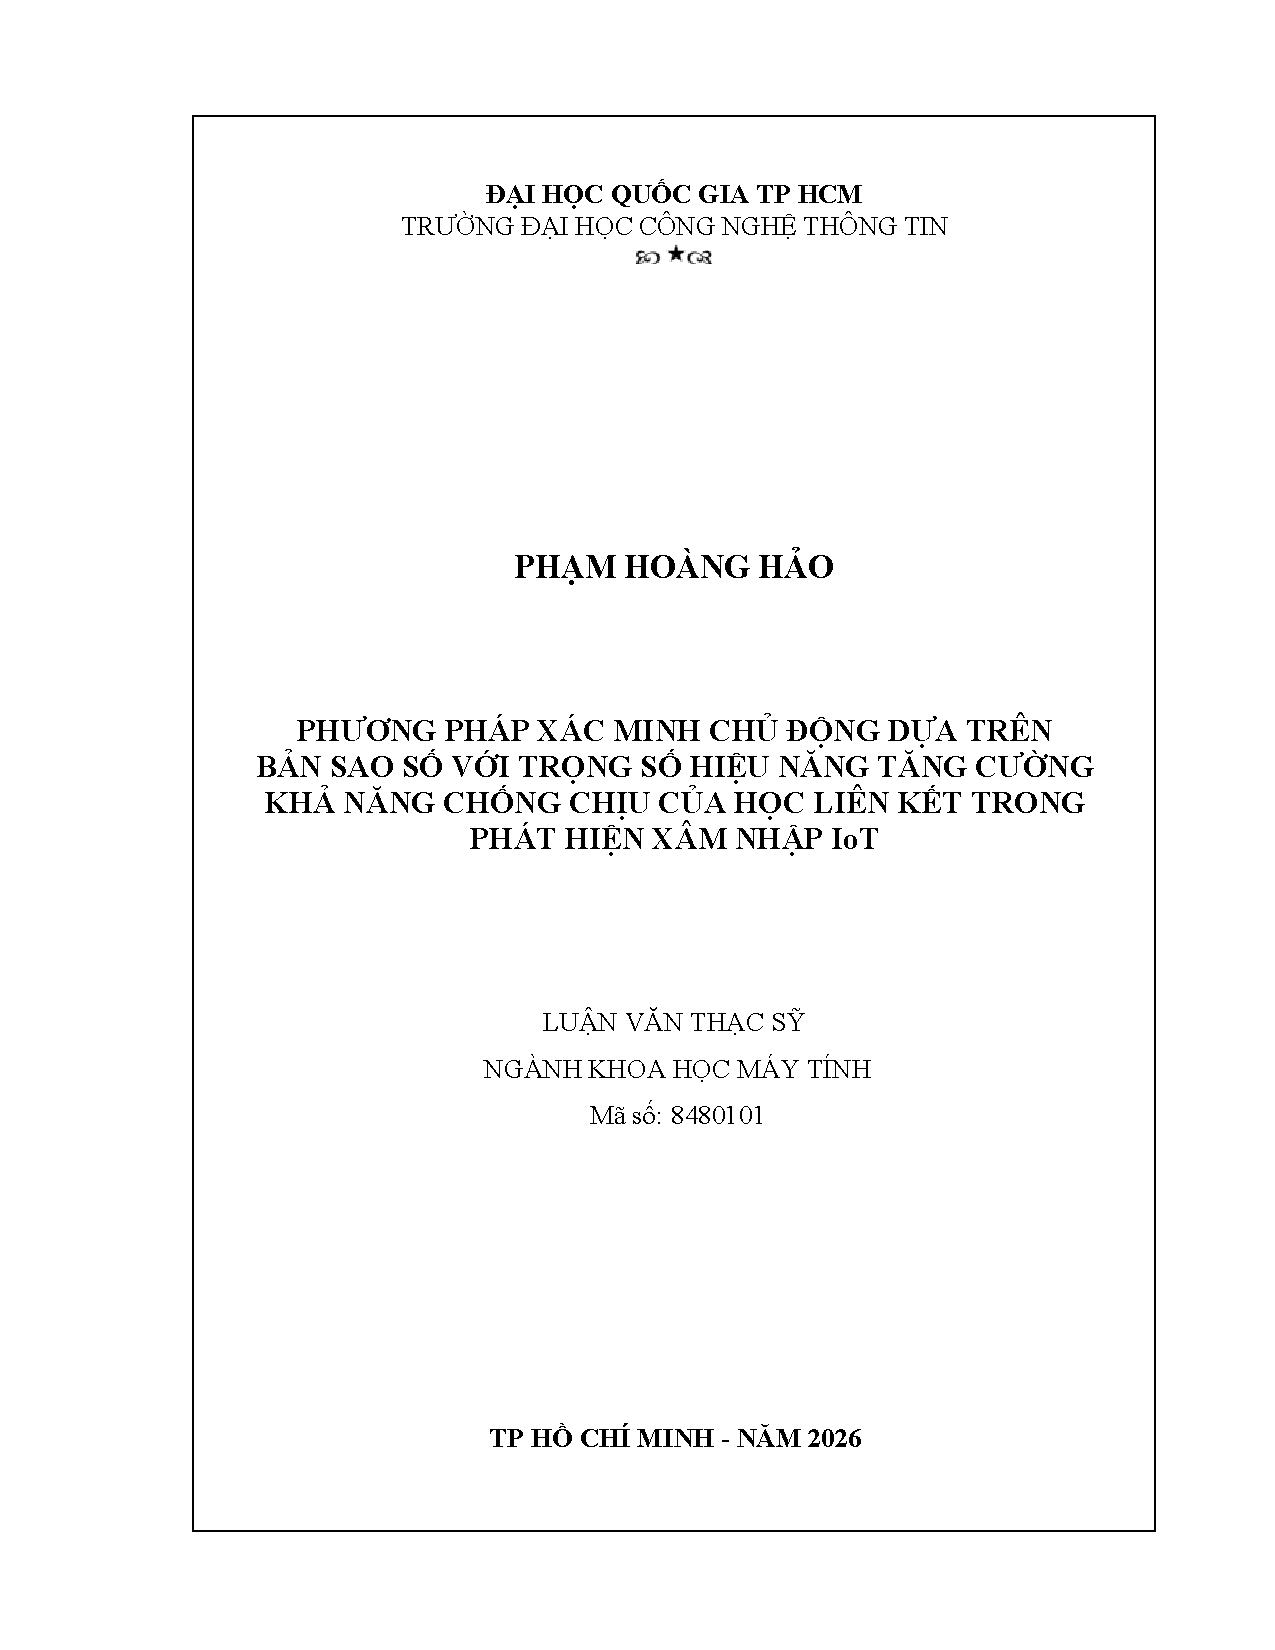
\includepdf[pages={1}, scale=0.99]{Covers/Front Cover.pdf}

\includepdf[pages={1}, scale=0.99]{Covers/Title Page Cover.pdf}

\begin{nopage}
\begin{pledges}

Tôi xin cam đoan: Luận văn tốt nghiệp với đề tài: "\textbf{Phương pháp xác minh chủ động dựa trên bản sao số với trọng số hiệu năng tăng cường khả năng chống chịu của học liên kết trong phát hiện xâm nhập IoT}" là công trình nghiên cứu của học viên, dưới sự hướng dẫn khoa học của Thầy TS. Phan Thế Duy.

Các trích dẫn, tham khảo trong luận văn đều được trích dẫn đầy đủ, ghi rõ nguồn gốc.

Học viên xin chịu hoàn toàn trách nhiệm nếu có bất kỳ sao chép không hợp lệ, vi phạm quy chế đào tạo.

\vspace{2cm}
\begin{tabular*}{\textwidth}{@{\extracolsep{\fill}}cc}
& TP. Hồ Chí Minh, tháng 4 năm 2026 \\
& Người thực hiện \\
& \\
& \\
& \\
& Phạm Hoàng Hảo \\
\end{tabular*}

\end{pledges}

\end{nopage}

\begin{nopage}
\begin{acknowledgements}

Lời đầu tiên, tôi xin bày tỏ lòng biết ơn sâu sắc đến Thầy TS. Phan Thế Duy. Trong suốt quá trình thực hiện luận văn, Thầy đã luôn tận tình chỉ bảo, hướng dẫn tôi không chỉ về chuyên môn mà còn về các kỹ năng nghiên cứu quan trọng.

Sự chỉ dạy và kinh nghiệm quý báu từ Thầy đã giúp tôi nhận thức rõ hơn về việc nghiên cứu khoa học đúng đắn, ý nghĩa của công việc này, cũng như cách trình bày, truyền tải kết quả nghiên cứu một cách hiệu quả. Sự tận tâm và kiến thức mà Thầy chia sẻ chính là động lực to lớn giúp tôi hoàn thành tốt luận văn này.

Tôi cũng xin gửi lời cảm ơn chân thành đến Phòng thí nghiệm An Toàn Thông Tin (InSec Lab) thuộc Trường Đại học Công nghệ Thông tin -- ĐHQG TP.HCM đã luôn hỗ trợ và đồng hành cùng tôi trong suốt quá trình thực hiện luận văn.

Cuối cùng, tôi xin gửi lời cảm ơn đến gia đình và bạn bè đã luôn động viên, tạo điều kiện thuận lợi để tôi hoàn thành luận văn.

Xin kính chúc tất cả mọi người sức khỏe và thành công.

\vspace{1cm}
\begin{tabular*}{\textwidth}{@{\extracolsep{\fill}}cc}
& TP. Hồ Chí Minh, tháng 4 năm 2026 \\
& Người thực hiện \\
& \\
& \\
& \\
& Phạm Hoàng Hảo \\
\end{tabular*}

\end{acknowledgements}

\end{nopage}

\frontmatter
\pagestyle{plain}
\mainmatter

\clearpage
\pagenumbering{arabic}
\setcounter{page}{1}

\clearpage
\phantomsection
\addcontentsline{toc}{chapter}{Mục lục}
\tableofcontents

\clearpage
\phantomsection
\addcontentsline{toc}{chapter}{Danh mục các hình vẽ, đồ thị}
\listoffigures

\clearpage
\phantomsection
\addcontentsline{toc}{chapter}{Danh mục các bảng}
\listoftables

\begin{abbreviations}{ll}
\textbf{FL} & Federated Learning \\
\addlinespace
\textbf{IDS} & Intrusion Detection System \\
\addlinespace
\textbf{IoT} & Internet of Things \\
\addlinespace
\textbf{IIoT} & Industrial Internet of Things \\
\addlinespace
\textbf{DT} & Digital Twin \\
\addlinespace
\textbf{DT-Guard} & Digital Twin Guard \\
\addlinespace
\textbf{DT-PW} & DT-Driven Performance Weighting \\
\addlinespace
\textbf{MLP} & Multilayer Perceptron \\
\addlinespace
\textbf{DDPM} & Denoising Diffusion Probabilistic Model \\
\addlinespace
\textbf{TabDDPM} & Tabular DDPM \\
\addlinespace
\textbf{GAN} & Generative Adversarial Network \\
\addlinespace
\textbf{CTGAN} & Conditional Tabular GAN \\
\addlinespace
\textbf{WGAN-GP} & Wasserstein GAN with Gradient Penalty \\
\addlinespace
\textbf{VAE} & Variational Autoencoder \\
\addlinespace
\textbf{SGD} & Stochastic Gradient Descent \\
\addlinespace
\textbf{FedAvg} & Federated Averaging \\
\addlinespace
\textbf{Non-IID} & Non-Independent and Identically Distributed \\
\addlinespace
\textbf{LIE} & A Little Is Enough \\
\addlinespace
\textbf{MPAF} & Model Poisoning Attacks based on Fake clients \\
\addlinespace
\textbf{Min-Max} & Min-Max Attack \\
\addlinespace
\textbf{Min-Sum} & Min-Sum Attack \\
\addlinespace
\textbf{GeoMed} & Geometric Median \\
\addlinespace
\textbf{MAD} & Median Absolute Deviation \\
\addlinespace
\textbf{MMD} & Maximum Mean Discrepancy \\
\addlinespace
\textbf{TSTR} & Train on Synthetic, Test on Real \\
\addlinespace
\textbf{DCR} & Distance to Closest Record \\
\addlinespace
\textbf{FPR} & False Positive Rate \\
\addlinespace
\textbf{DR} & Detection Rate \\
\addlinespace
\textbf{F1} & F1-Score \\
\addlinespace
\textbf{ReLU} & Rectified Linear Unit \\
\addlinespace
\textbf{NIDS} & Network-based IDS \\
\addlinespace
\textbf{HIDS} & Host-based IDS \\
\addlinespace
\textbf{GPU} & Graphics Processing Unit \\
\addlinespace
\textbf{CPU} & Central Processing Unit \\
\addlinespace
\textbf{DDoS} & Distributed Denial of Service \\
\addlinespace
\textbf{DoS} & Denial of Service \\
\end{abbreviations}


\begin{abstract}
\addchaptertocentry{\tomtatname}
Luận văn đề xuất DT-Guard --- hệ thống phòng thủ chủ động dựa trên Digital Twin cho Federated Learning (FL) trong phát hiện xâm nhập IoT. Khác với các phương pháp phòng thủ thụ động dựa trên phân tích tham số, DT-Guard xây dựng môi trường kiểm chứng hành vi bằng Digital Twin với pipeline kiểm định 4 lớp và Trust-Score. Thông qua A/B Testing năm mô hình sinh dữ liệu, luận văn đánh giá và lựa chọn TabDDPM làm bộ sinh dữ liệu thách thức phù hợp nhất cho môi trường kiểm chứng. Ngoài ra, cơ chế DT-PW (DT-Driven Performance Weighting) với Effort Gate định lượng đóng góp tri thức và loại bỏ free-rider.

Thực nghiệm trên hai bộ dữ liệu CIC-IoT-2023 (34 lớp, 39 đặc trưng) và ToN-IoT (10 lớp, 10 đặc trưng) với 9 phương pháp baseline và 5 loại tấn công (Backdoor, LIE, Min-Max, Min-Sum, MPAF) ở bốn tỉ lệ client độc hại (10\%--50\%) cho thấy: (1) DT-Guard đạt FPR = 0\% trên cả hai tập dữ liệu ở mọi kịch bản; (2) Detection Rate đạt 89,5\%--98,3\% trên CIC-IoT-2023 và 90\%--100\% trên ToN-IoT; (3) DT-PW phát hiện 100\% free-rider (trọng số = 0); (4) Overhead chỉ 80,8 ms/round (\textless 1\%) và peak memory 485 MB. Kết quả cốt lõi đã được đệ trình tại hội nghị IEEE ICCE 2026 {[}23{]}, hiện đang chờ duyệt. Luận văn chứng minh nguyên lý kiểm chứng hành vi chủ động vượt trội hơn phân tích tham số thụ động, và nguyên lý này tổng quát không phụ thuộc dataset hay kiến trúc mô hình IDS cụ thể. Lỗ hổng của các phương pháp thụ động mang tính cấu trúc: cùng một baseline thất bại trước cùng loại tấn công ở cả hai môi trường thử nghiệm.
\end{abstract}


\pagestyle{thesis}
\setstretch{1.5}
% Chapter 1
\chapter{MỞ ĐẦU}
\label{Chapter1}

\section{Động lực nghiên cứu}
Trong bối cảnh Cách mạng Công nghiệp 4.0, Internet of Things (IoT) đã trở thành một phần không thể thiếu trong nhiều lĩnh vực như y tế thông minh, giao thông đô thị, nhà thông minh và công nghiệp. Sự phát triển chóng mặt của IoT cũng kéo theo thách thức nghiêm trọng về an toàn thông tin: tấn công mạng nhắm vào thiết bị IoT tăng 87\% giai đoạn 2022--2024, với các hình thức ngày càng tinh vi và đa dạng.

Hệ thống phát hiện xâm nhập (Intrusion Detection System - IDS) dựa trên học máy và học sâu đóng vai trò trọng yếu trong việc tự động phát hiện hoạt động bất thường trong lưu lượng mạng. Tuy nhiên, cách tiếp cận truyền thống yêu cầu tập trung hóa dữ liệu tại máy chủ trung tâm, vi phạm quyền riêng tư dữ liệu IoT. Hơn nữa, việc tập trung hóa còn gặp rào cản về băng thông, độ trễ và vấn đề pháp lý khi chuyển dữ liệu qua biên giới.

Học liên kết (Federated Learning - FL), được giới thiệu bởi McMahan và cộng sự năm 2017 {[}9{]}, cho phép nhiều client cùng huấn luyện mô hình chung mà không cần chia sẻ dữ liệu thô. Trong ngữ cảnh IoT IDS, FL vừa bảo vệ quyền riêng tư, vừa tận dụng nguồn dữ liệu phân tán. Tuy nhiên, trong môi trường IoT, dữ liệu thường có đặc tính Non-IID (phân bố không đồng nhất), tạo điều kiện cho các tấn công đầu độc (poisoning) và backdoor trở nên hiệu quả hơn.

Nhiều phương pháp phòng thủ đã được đề xuất, nhưng phân tích đối sánh toàn diện trong DT-BFL {[}5{]} cho thấy kết luận đáng quan ngại: không có phương pháp nào duy trì hiệu năng tốt trước tất cả các loại tấn công. Từ nhu cầu thực tế này, đề tài "Phương pháp xác minh chủ động dựa trên bản sao số với trọng số hiệu năng tăng cường khả năng chống chịu của học liên kết trong phát hiện xâm nhập IoT" được thực hiện nhằm xây dựng khung phòng thủ DT-Guard, trong đó Digital Twin đóng vai trò kiểm chứng hành vi chủ động, kết hợp cơ chế DT-PW để định lượng đóng góp tri thức và loại bỏ free-rider.

\section{Phát biểu bài toán}
Xét hệ thống FL-IDS gồm $N$ client cùng huấn luyện mô hình phát hiện xâm nhập toàn cục $\mathbf{w}$ qua $R$ vòng lặp. Trong đó có $K$ client độc hại (tập $M$, $K$ không biết trước) và $N - K$ client lành tính (tập $B$). Mỗi client sở hữu dữ liệu cục bộ có phân phối Non-IID theo Dirichlet($\alpha$).

Tại mỗi round, server nhận bản cập nhật từ N client nhưng không truy cập được dữ liệu thô. Server cần thiết kế cơ chế phòng thủ đạt ba yêu cầu: (1) mô hình toàn cục duy trì Accuracy cao bất chấp client độc hại; (2) phát hiện chính xác client độc hại với Detection Rate cao và False Positive Rate (FPR) thấp; (3) trọng số tổng hợp phản ánh đúng đóng góp tri thức, gán trọng số bằng 0 cho free-rider --- client không huấn luyện, chỉ sao chép mô hình toàn cục.

Ràng buộc: server không truy cập dữ liệu thô; overhead nhỏ hơn 1\% thời gian mỗi round; hoạt động hiệu quả trên nhiều loại tấn công và nhiều tỉ lệ $K/N$ (10\%--50\%).

\section{Các thách thức}
Phân tích đối sánh toàn diện các phương pháp phòng thủ hiện có --- gồm Krum {[}2{]}, Median {[}18{]}, Trimmed Mean {[}18{]}, GeoMed {[}12{]}, SignGuard {[}16{]}, ClipCluster {[}19{]}, LUP {[}5{]}, và PoC {[}22{]} --- cho thấy ba thách thức cốt lõi:

\textbf{Thách thức 1: Phòng thủ dễ bị qua mặt.} Tất cả phương pháp hiện tại đều dựa trên phân tích tham số thụ động (passive parameter inspection), chỉ đánh giá hình thái tham số thay vì kiểm chứng hành vi suy luận thực tế. Các tấn công tối ưu ngược như LIE {[}1{]}, Min-Max/Min-Sum {[}15{]} được thiết kế đặc biệt để giữ tham số trong vùng thống kê bình thường. Không có phương pháp nào duy trì Detection Rate cao và FPR thấp đồng thời trên tất cả các loại tấn công.

\textbf{Thách thức 2: Nhầm lẫn Non-IID với đầu độc.} Phân tích tham số thụ động dễ nhầm lẫn giữa sai lệch tự nhiên do Non-IID và hành vi đầu độc cố tình. Client lành tính có dữ liệu thiên lệch cũng có tham số khác với mô hình toàn cục, bị các phương pháp như LUP và PoC loại nhầm.

\textbf{Thách thức 3: Chưa đo được đóng góp tri thức thực tế.} FedAvg {[}9{]} gán trọng số theo số lượng mẫu, không phản ánh chất lượng. Cơ chế Trust Score trong LUP {[}5{]} và PoC {[}22{]} dựa trên khoảng cách tham số, vô tình thưởng cho free-rider --- client không đóng góp nhưng có tham số gần mô hình toàn cục. HSDPS {[}21{]} sử dụng Shapley Value nhưng chi phí theo cấp số mũ.

\section{Mục tiêu và phạm vi nghiên cứu}
\textbf{Mục tiêu:}

\textbf{(1)} Xây dựng khung DT-Guard tích hợp Digital Twin làm môi trường kiểm chứng hành vi chủ động. Digital Twin đóng vai trò sandbox tách biệt để chủ động kiểm chứng năng lực suy luận của từng mô hình cục bộ trên dữ liệu thách thức được kiểm soát, thông qua pipeline kiểm định 4 lớp.

\textbf{(2)} Thiết kế cơ chế DT-PW (DT-Driven Performance Weighting) để định lượng đóng góp tri thức thực tế và phát hiện free-rider, kết hợp Effort Gate xác định ngưỡng thích ứng.

\textbf{(3)} Đánh giá toàn diện trên hai bộ dữ liệu IoT IDS tiêu chuẩn (CIC-IoT-2023 {[}11{]} và ToN-IoT), so sánh với chín phương pháp phòng thủ đại diện hiện nay.

\textbf{Phạm vi nghiên cứu:}

\begin{itemize}
\item
  Hai bộ dữ liệu: CIC-IoT-2023 (34 lớp, 39 đặc trưng) và ToN-IoT (10 lớp, 10 đặc trưng).
\item
  Cấu hình FL: 20 client, phân bổ Non-IID theo Dirichlet ($\alpha$ = 0,5), 20 vòng lặp, mô hình IoTAttackNet (MLP: $256\rightarrow128\rightarrow64$).
\item
  Năm loại tấn công: Backdoor, LIE {[}1{]}, Min-Max {[}15{]}, Min-Sum {[}15{]}, MPAF {[}3{]}, ở bốn tỷ lệ client độc hại (10\%, 20\%, 40\%, 50\%).
\item
  Chín phương pháp đối sánh: FedAvg, Krum, Median, Trimmed Mean, GeoMed, SignGuard, ClipCluster, LUP, PoC.
\item
  Giới hạn: không đánh giá membership inference, model extraction hay evasion attack; không thử nghiệm trên mạng IoT thực tế quy mô lớn; không tích hợp Blockchain.
\end{itemize}

\section{Đóng góp của luận văn}
Luận văn đóng góp năm kết quả chính:

\textbf{(1) Khung DT-Guard với pipeline kiểm định hành vi 4 lớp.} Chuyển paradigm từ phân tích tham số thụ động sang kiểm chứng hành vi chủ động bằng Digital Twin, đánh giá trực tiếp năng lực suy luận của mô hình trên dữ liệu thách thức thay vì chỉ phân tích hình thái tham số.

\textbf{(2) Cơ chế DT-PW với Effort Gate.} Đo prediction divergence giữa mô hình cục bộ và mô hình toàn cục để định lượng đóng góp tri thức. Effort Gate tự động loại bỏ free-rider (trọng số = 0), giải quyết vấn đề Trust Score vô tình thưởng cho client không đóng góp.

\textbf{(3) Bộ sinh dữ liệu thách thức dựa trên TabDDPM {[}7{]}.} Đạt kết quả tốt nhất qua A/B Testing năm mô hình sinh, đảm bảo chất lượng kiểm thử cho pipeline.

\textbf{(4) Đánh giá toàn diện chứng minh tính tổng quát hóa.} DT-Guard duy trì FPR = 0\% trên cả CIC-IoT-2023 và ToN-IoT qua 40 kịch bản, trong khi mọi baseline đều thất bại trước ít nhất một loại tấn công.

\textbf{(5) Overhead thấp, phù hợp IoT.} Overhead chiếm dưới 1\% tổng thời gian round, peak memory thấp nhất trong tất cả phương pháp.

\textbf{Ý nghĩa khoa học:} Luận văn chứng minh nguyên lý kiểm chứng hành vi chủ động vượt trội hơn phân tích tham số thụ động, và nguyên lý này tổng quát không phụ thuộc dataset hay kiến trúc mô hình IDS cụ thể. Lỗ hổng của các phương pháp thụ động mang tính cấu trúc: cùng một baseline thất bại trước cùng loại tấn công ở cả hai môi trường thử nghiệm.

\textbf{Ý nghĩa thực tiễn:} Framework triển khai được cho hệ thống FL-IDS thực tế với overhead không đáng kể, phù hợp môi trường tài nguyên hạn chế. Kết quả cốt lõi đã đệ trình tại hội nghị IEEE ICCE 2026 {[}23{]}.

\section{Bố cục của luận văn}
Ngoài Chương mở đầu, luận văn được cấu trúc thành năm chương:

\textbf{Chương 2. Tổng quan về vấn đề nghiên cứu} --- phân tích các công trình nghiên cứu liên quan về IoT, IDS, FL, tấn công poisoning/backdoor, phương pháp phòng thủ hiện có, Digital Twin trong FL-IoT, chỉ ra ba thách thức và xác định mục tiêu, phương pháp nghiên cứu.

\textbf{Chương 3. Cơ sở lý thuyết và công nghệ nền tảng} --- trình bày chi tiết Federated Learning, cơ chế kỹ thuật các tấn công, Digital Twin, mô hình sinh dữ liệu dạng bảng, mô hình IDS IoTAttackNet, và hai bộ dữ liệu thực nghiệm.

\textbf{Chương 4. Đề xuất hệ thống DT-Guard} --- kiến trúc tổng thể, bộ sinh TabDDPM, pipeline kiểm định 4 lớp với Trust-Score, cơ chế DT-PW với Effort Gate, phân tích lý thuyết.

\textbf{Chương 5. Thực nghiệm và đánh giá} --- thiết lập, ba kịch bản thực nghiệm (phòng thủ, bộ sinh, free-rider), phân tích overhead, bàn luận tổng hợp.

\textbf{Chương 6. Kết luận và khuyến nghị} --- tổng kết, đóng góp khoa học, hạn chế, hướng phát triển tiếp theo.

% Chapter 2
\chapter{TỔNG QUAN VỀ VẤN ĐỀ NGHIÊN CỨU}
\label{Chapter2}

Chương này tổng quan về các khái niệm nền tảng và tình trạng nghiên cứu, gồm: IoT và thách thức an toàn thông tin, hệ thống IDS, Federated Learning, các tấn công poisoning/backdoor, phương pháp phòng thủ hiện có, và Digital Twin trong FL-IoT.

\section{Giới thiệu về Internet of Things (IoT)}

\subsection{Khái niệm và kiến trúc IoT}
Internet of Things (IoT) là một mạng lưới các đối tượng vật lý (thiết bị, phương tiện, tòa nhà và các vật phẩm khác) được nhúng cảm biến, phần mềm, và khả năng kết nối mạng, cho phép các đối tượng này thu thập và trao đổi dữ liệu. Khái niệm IoT đã phát triển từ những nghiên cứu ban đầu trong thập niên 1990 và sau đó được mở rộng nhờ sự phát triển mạnh mẽ của công nghệ kết nối không dây, cảm biến giá rẻ, và điện toán đám mây.

Kiến trúc IoT thường được chia thành ba lớp chính:

\textbf{Lớp Perception (Cảm nhận):} Đây là lớp thấp nhất trong kiến trúc IoT, bao gồm các cảm biến và thiết bị thu thập dữ liệu từ môi trường vật lý. Các cảm biến này có thể đo nhiều loại dữ liệu như nhiệt độ, độ ẩm, chuyển động, hình ảnh, âm thanh, lưu lượng mạng, và nhiều tham số khác. Tại lớp này, dữ liệu được thu thập sơ bộ, đôi khi được tiền xử lý trước khi chuyển lên lớp cao hơn.

\textbf{Lớp Network (Mạng):} Lớp này đảm bảo kết nối và truyền tải dữ liệu giữa các thiết bị IoT và các hệ thống xử lý. Các giao thức kết nối đa dạng tùy thuộc vào yêu cầu về băng thông, độ trễ, và tiêu thụ năng lượng: Wi-Fi, Bluetooth, Zigbee, LoRaWAN, 4G/5G, và các giao thức chuyên dụng khác. Lớp mạng cũng đảm bảo các dịch vụ định tuyến, bảo mật, và quản lý kết nối.

\textbf{Lớp Application (Ứng dụng):} Lớp cao nhất nơi dữ liệu từ IoT được xử lý, phân tích, và sử dụng cho các mục đích cụ thể. Các ứng dụng IoT có thể trong nhiều lĩnh vực như nhà thông minh (điều khiển đèn, nhiệt độ), y tế thông minh (theo dõi bệnh nhân, thiết bị y tế), giao thông thông minh (quản lý đèn tín hiệu, giám sát giao thông), công nghiệp 4.0 (giám sát sản xuất, bảo trì dự đoán), và nông nghiệp chính xác (theo dõi đất, thời tiết, tự động tưới).

\begin{figure}[H]
    \centering
    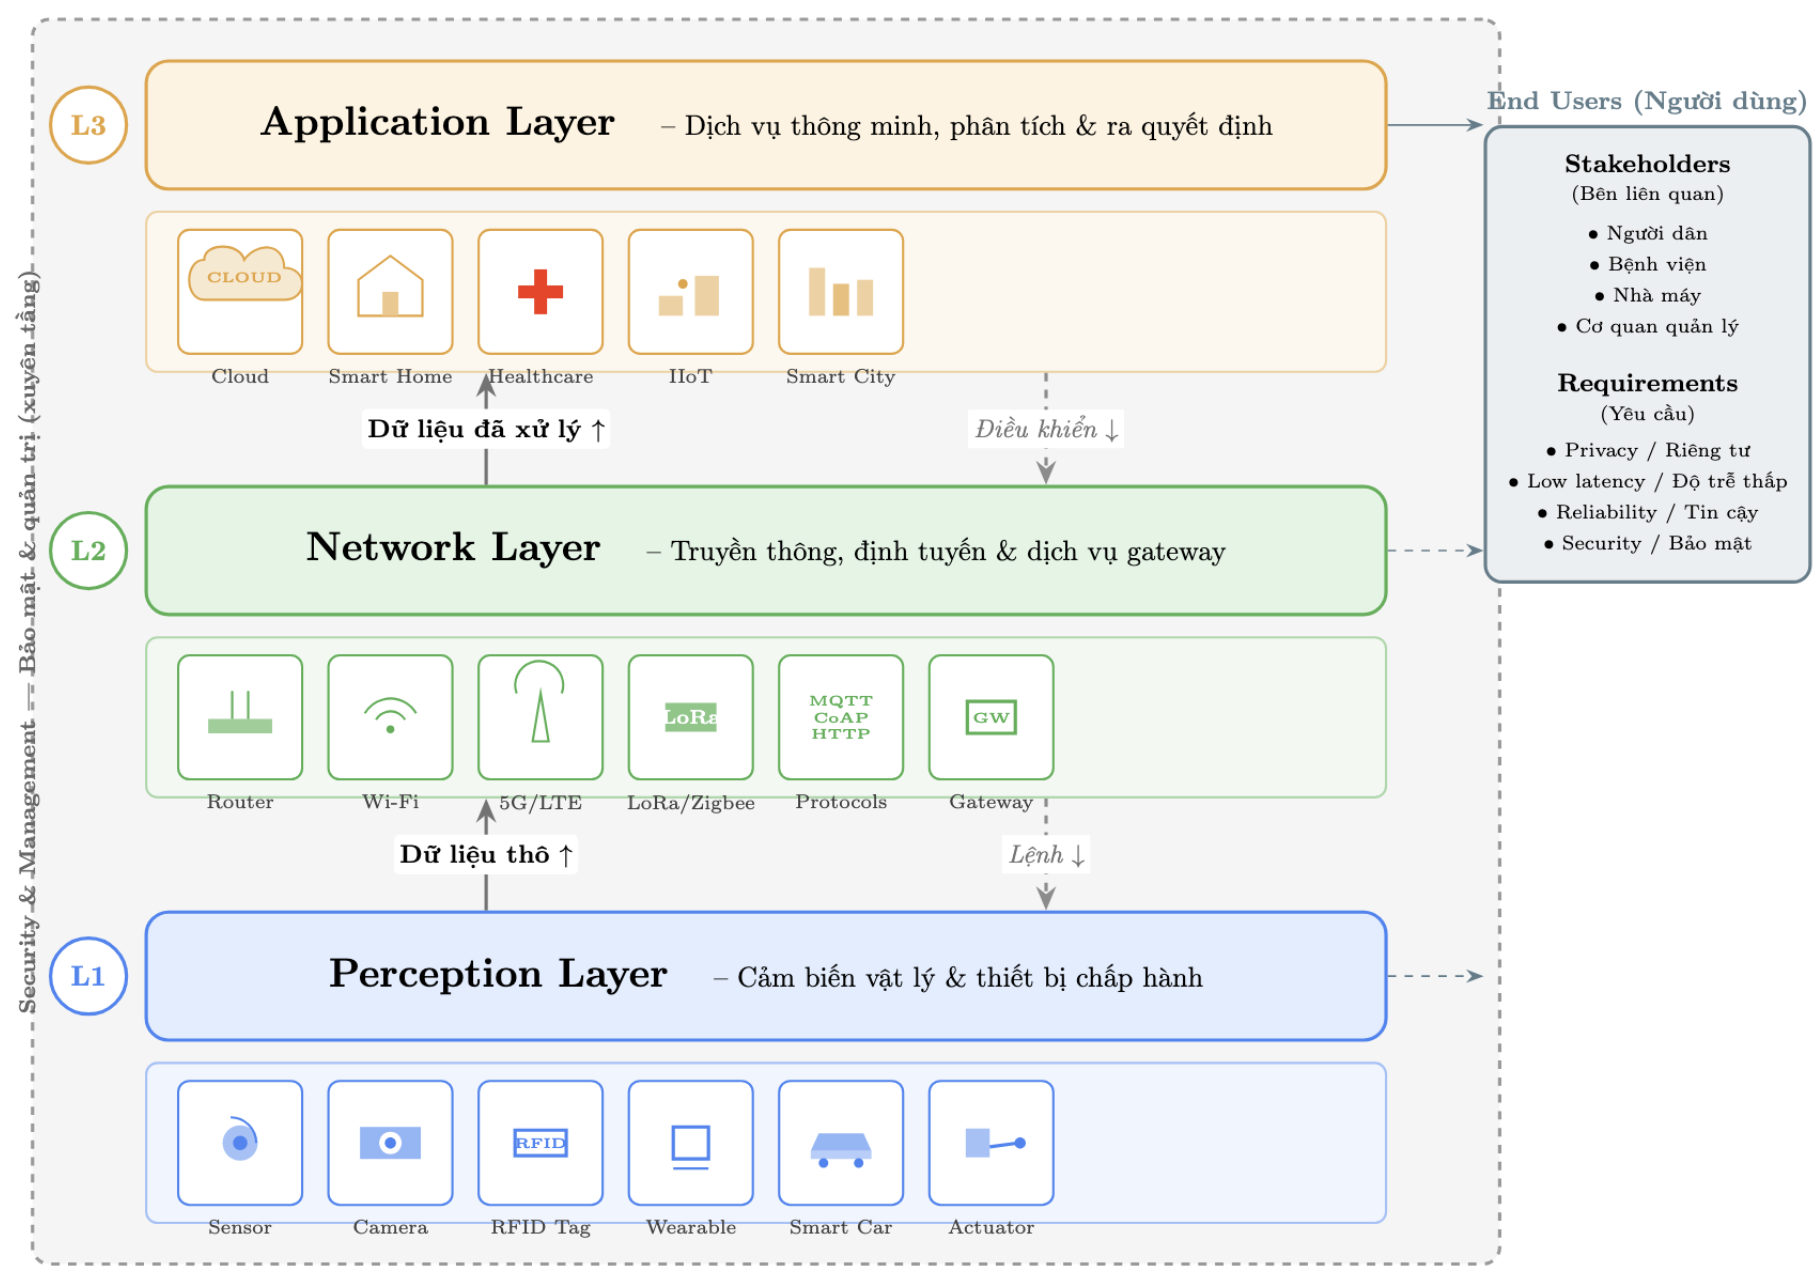
\includegraphics[width=0.85\linewidth]{Figures/fig_2_1_kien_truc_iot_3_lop.png}
    \caption{Kiến trúc IoT 3 lớp}
\end{figure}

Các thiết bị và giao thức IoT phổ biến hiện nay rất đa dạng. Về thiết bị, có thể kể đến: cảm biến môi trường (nhiệt độ, độ ẩm, áp suất), thiết bị giám sát (camera, microphone), thiết bị đeo (smartwatch, fitness tracker), thiết bị gia dụng thông minh (tủ lạnh, máy giặt, điều hòa), thiết bị công nghiệp (robot, máy móc tự động), và xe thông minh. Về giao thức, có các giao thức tầm ngắn năng lượng thấp như Zigbee, Z-Wave, LoRaWAN cho các ứng dụng cảm biến; Bluetooth và BLE cho thiết bị đeo và gia dụng; Wi-Fi cho các ứng dụng băng thông cao như camera giám sát; và mạng di động 4G/5G cho các ứng dụng cần độ phủ sóng rộng.

\subsection{Thách thức an toàn thông tin trong IoT}
Internet of Things mang lại nhiều lợi ích nhưng cũng đối mặt với nhiều thách thức an toàn thông tin đặc thù. Các đặc tính của IoT tạo điều kiện cho các mối đe dọa an toàn thông tin mới hoặc làm gia tăng mức độ nghiêm trọng của các mối đe dọa đã tồn tại.

\textbf{Đặc tính của IoT:}

IoT có nhiều đặc tính khác biệt với các hệ thống truyền thống. \textbf{Số lượng thiết bị lớn}: Hệ thống IoT có thể bao gồm hàng triệu thiết bị phân tán trên diện tích rộng. \textbf{Tài nguyên hạn chế}: Nhiều thiết bị IoT có năng lượng, bộ nhớ, và khả năng xử lý hạn chế do yêu cầu kích thước nhỏ, tiêu thụ năng lượng thấp, và chi phí rẻ. \textbf{Môi trường không an toàn}: Các thiết bị IoT thường được triển khai trong môi trường công cộng, dễ bị tiếp cận vật lý để thao túng hoặc tấn công. \textbf{Kết nối đa dạng}: Sự kết nối thông qua nhiều giao thức khác nhau tạo ra nhiều điểm tấn công tiềm năng.

\textbf{Các mối đe dọa an toàn thông tin trong IoT:}

Các mối đe dọa an toàn thông tin trong IoT rất đa dạng và có thể được phân loại theo nhiều tiêu chí. Theo lớp tấn công: \textbf{Tấn công vật lý}: tiếp cận trực tiếp thiết bị để thao túng, sao chép dữ liệu, hoặc thay thế thiết bị giả mạo. \textbf{Tấn công mạng}: tấn công vào giao thức và kết nối mạng như đánh giá lại, chèn gói tin, từ chối dịch vụ (DoS/DDoS). \textbf{Tấn công phần mềm}: khai thác lỗ hổng trong phần mềm, firmware, hoặc hệ điều hành của thiết bị IoT. \textbf{Tấn công mã hóa}: tấn công vào cơ chế mã hóa và xác thực để truy cập trái phép dữ liệu hoặc hệ thống.

Theo mục đích: \textbf{Tấn công phát hiện xâm nhập}: cố gắng phát hiện và thu thập thông tin về hệ thống IDS để lẩn tránh. \textbf{Tấn công lấy cắp dữ liệu}: đánh cắp dữ liệu cảm biến hoặc thông tin cá nhân từ thiết bị IoT. \textbf{Tấn công từ chối dịch vụ}: làm cho hệ thống không thể phục vụ người dùng hợp pháp. \textbf{Tấn công điều khiển}: chiếm quyền điều khiển thiết bị hoặc hệ thống để thực hiện hành vi nguy hiểm.

\textbf{Yêu cầu bảo vệ quyền riêng tư dữ liệu:}

Dữ liệu từ thiết bị IoT thường chứa thông tin nhạy cảm về hành vi người dùng, hoạt động gia đình, hoặc dữ liệu y tế. Việc bảo vệ quyền riêng tư dữ liệu IoT là một yêu cầu quan trọng, cả về mặt pháp lý và đạo đức. Các quy định pháp lý như GDPR tại Châu Âu, CCPA tại Mỹ, và các quy định về bảo vệ dữ liệu cá nhân khác hạn chế việc thu thập và xử lý dữ liệu cá nhân mà không có sự đồng ý của người dùng. Hệ thống phát hiện xâm nhập truyền thống thường yêu cầu tập trung hóa dữ liệu để huấn luyện mô hình, điều này có thể xung đột với các quy định về quyền riêng tư và tạo ra rào cản pháp lý cho việc triển khai.

\section{Hệ thống phát hiện xâm nhập mạng (Intrusion Detection System)}

\subsection{Khái niệm và nguyên lý hoạt động của IDS}
Hệ thống phát hiện xâm nhập (Intrusion Detection System - IDS) là một thiết bị hoặc ứng dụng phần mềm giám sát mạng hoặc hệ thống để tìm các hoạt động vi phạm chính sách hoặc hoạt động bất thường. IDS là một thành phần quan trọng trong hệ thống an toàn thông tin, đóng vai trò tuyến phòng thủ chủ động để phát hiện các cuộc tấn công hoặc hành vi bất thường kịp thời.

\textbf{Quy trình hoạt động cơ bản của IDS:}

Quy trình hoạt động cơ bản của IDS gồm các bước sau:

\textbf{Bước 1: Thu thập dữ liệu.} IDS thu thập dữ liệu từ mạng hoặc hệ thống thông qua nhiều nguồn khác nhau như network packets, system logs, process activities, và các sự kiện hệ thống khác. Dữ liệu thu thập được bao gồm thông tin về địa chỉ IP, cổng, giao thức, nội dung gói tin, thời gian, và nhiều thông tin khác.

\textbf{Bước 2: Phân tích dữ liệu.} Dữ liệu thu thập được phân tích theo các quy tắc hoặc mô hình học được. Phân tích có thể được thực hiện theo thời gian thực (real-time) để phát hiện ngay lập tức các cuộc tấn công, hoặc được thực hiện theo thời gian rời rạc (offline) để phân tích lại các log và phát hiện các cuộc tấn công đã xảy ra.

\textbf{Bước 3: Phát hiện các dấu hiệu.} Từ việc phân tích dữ liệu, IDS phát hiện các dấu hiệu của tấn công hoặc hành vi bất thường. Các dấu hiệu này có thể là các mẫu tấn công đã biết (signature), các hoạt động bất thường so với hành vi bình thường, hoặc các kết hợp của cả hai.

\textbf{Bước 4: Kích hoạt cảnh báo hoặc phản hồi.} Khi phát hiện dấu hiệu tấn công hoặc hành vi bất thường, IDS kích hoạt cảnh báo hoặc phản hồi tự động. Cảnh báo được gửi cho quản trị viên qua email, SMS, hoặc các kênh khác. Phản hồi tự động bao gồm chặn kết nối, cô lập hệ thống, hoặc thực hiện các hành động phòng thủ khác.

\textbf{Vai trò của IDS trong hệ thống an toàn thông tin:}

IDS có ý nghĩa quan trọng trong hệ thống an toàn thông tin như một lớp phòng thủ chủ động. Khác với tường lửa (firewall) chỉ chặn các kết nối dựa trên quy tắc được định nghĩa trước, IDS có thể phát hiện các cuộc tấn công mới và các hành vi bất thường chưa có trong quy tắc. IDS kết hợp với các thành phần an toàn khác như tường lửa, hệ thống chống virus, và hệ thống giám sát để tạo thành một hệ thống an toàn toàn diện.

\subsection{Phân loại IDS}
IDS có thể được phân loại theo nhiều tiêu chí khác nhau tùy thuộc vào phương pháp phát hiện và vị trí triển khai.

\textbf{Theo phương pháp phát hiện:}

\textbf{Signature-based IDS} (hay còn gọi là Misuse Detection) sử dụng các mẫu tấn công đã biết (signatures) để phát hiện các cuộc tấn công tương tự. Các signature có thể là chuỗi byte đặc thù, mẫu gói tin, hoặc các đặc trưng hành vi đã biết. Khi dữ liệu mạng khớp với một signature đã biết, IDS kích hoạt cảnh báo về cuộc tấn công tương ứng. Ưu điểm của phương pháp này là có độ chính xác cao cho các tấn công đã biết vì dựa trên pattern đã được xác nhận. Nhược điểm là không phát hiện được các tấn công mới (zero-day) vì không có signature tương ứng.

\textbf{Anomaly-based IDS} xây dựng mô hình hành vi bình thường và phát hiện các hoạt động lệch khỏi mô hình này. Mô hình hành vi bình thường được xây dựng từ việc phân tích dữ liệu trong trạng thái không bị tấn công (baseline). Khi có hoạt động lệch khỏi mô hình bình thường, IDS kích hoạt cảnh báo về hoạt động bất thường. Ưu điểm của phương pháp này là có khả năng phát hiện các tấn công mới (zero-day) vì không phụ thuộc vào signature đã biết. Nhược điểm là tỷ lệ dương tính giả cao (FPR) vì các hành vi hợp pháp bất thường cũng bị báo cáo là tấn công.

\textbf{Hybrid IDS} kết hợp cả hai phương pháp trên để tận dụng ưu điểm của từng phương pháp, giảm nhược điểm của từng phương pháp riêng lẻ. Hybrid IDS sử dụng cả signature-based detection cho các tấn công đã biết và anomaly-based detection cho các tấn công mới, tạo thành một hệ thống phát hiện toàn diện hơn.

\textbf{Theo vị trí triển khai:}

\textbf{Network-based IDS (NIDS)} được triển khai tại các điểm chiến lược của mạng để giám sát lưu lượng mạng. NIDS phân tích các gói tin đi qua mạng để phát hiện các cuộc tấn công như scan port, DDoS, và truy cập trái phép. NIDS có thể được triển khai ở nhiều vị trí như gateway, router, hoặc các điểm trung gian khác trong mạng.

\textbf{Host-based IDS (HIDS)} được cài đặt trên từng thiết bị hoặc máy chủ để giám sát hoạt động hệ thống, tệp tin, và quy trình. HIDS phân tích các log hệ thống, hoạt động tệp tin, và các sự kiện khác để phát hiện các cuộc tấn công như thay đổi tệp hệ thống, thực thi mã độc, và leo thang đặc quyền. HIDS phù hợp để phát hiện các cuộc tấn công đã xâm nhập vào hệ thống.

\subsection{Hạn chế của IDS truyền thống trong ngữ cảnh IoT}
Mặc dù IDS là công cụ quan trọng trong bảo mật mạng, việc triển khai IDS truyền thống trong môi trường IoT gặp nhiều thách thức đặc thù. Hạn chế cốt lõi nhất là \textbf{cần tập trung hóa dữ liệu} để huấn luyện mô hình.

Về quyền riêng tư, dữ liệu từ thiết bị IoT thường chứa thông tin nhạy cảm. Các quy định pháp lý như GDPR tại Châu Âu, CCPA tại Mỹ, và các quy định về bảo vệ dữ liệu cá nhân khác hạn chế việc thu thập và xử lý dữ liệu cá nhân mà không có sự đồng ý của người dùng. Việc tập trung hóa dữ liệu từ nhiều thiết bị IoT về một server trung tâm có thể vi phạm các quy định này.

Về băng thông, việc truyền toàn bộ dữ liệu lưu lượng mạng về server trung tâm đòi hỏi băng thông lớn và có độ trễ cao. Trong môi trường IoT với số lượng thiết bị khổng lồ và dữ liệu liên tục, việc này không chỉ tốn kém mà còn ảnh hưởng đến khả năng phản ứng thời gian thực của hệ thống IDS. Đặc biệt trong các ứng dụng cần phản ứng nhanh như giám sát y tế hoặc hệ thống giao thông, độ trễ do truyền dữ liệu về server là không thể chấp nhận được.

Về tính khả thi, các hệ thống yêu cầu phản ứng gần tức thời để phát hiện và ngăn chặn tấn công không thể sử dụng IDS truyền thống tập trung hóa, do đó cần phương pháp phân tán như Federated Learning.

Về tính toán và lưu trữ, việc xử lý dữ liệu từ hàng triệu thiết bị IoT đòi hỏi tài nguyên tính toán và lưu trữ rất lớn. Điều này làm tăng chi phí vận hành và có thể không khả thi với các hạ tầng hiện có.

Federated Learning xuất hiện như một giải pháp hứa hẹn giải quyết các vấn đề này bằng cách cho phép các thiết bị IoT cùng huấn luyện mô hình IDS mà không cần chia sẻ dữ liệu thô.

\section{Tổng quan về Học liên kết (Federated Learning)}

\subsection{Khái niệm và nguyên lý FL}
Học liên kết (Federated Learning - FL) là một phương pháp học máy phân tán cho phép nhiều thiết bị hoặc client cùng tham gia huấn luyện một mô hình chung mà không cần chia sẻ dữ liệu thô. Khái niệm này được giới thiệu lần đầu bởi McMahan và cộng sự năm 2017 {[}9{]} và nhanh chóng trở thành một trong những phương pháp quan trọng nhất trong các ứng dụng yêu cầu bảo vệ quyền riêng tư dữ liệu.

Mỗi vòng FL diễn ra theo năm bước: (1) server khởi tạo và phân phối mô hình toàn cục cho các client; (2) mỗi client huấn luyện cục bộ trên dữ liệu riêng; (3) client gửi tham số hoặc gradient cập nhật về server; (4) server tổng hợp bằng thuật toán FedAvg (lấy trung bình có trọng số của tham số từ các client, trọng số tỷ lệ với số lượng mẫu); (5) server phân phối lại mô hình toàn cục mới. Quy trình lặp lại cho đến khi hội tụ. Chi tiết toán học của FedAvg được trình bày tại Mục 3.1.2.

FedAvg hoạt động hiệu quả khi dữ liệu IID giữa các client, nhưng gặp thách thức khi dữ liệu Non-IID, tình huống phổ biến trong môi trường IoT.

\subsection{FL trong ngữ cảnh IoT IDS}
\textbf{Lợi ích của FL cho IoT IDS:}

Trong ngữ cảnh phát hiện xâm nhập mạng cho IoT (IoT IDS), FL mang lại nhiều lợi ích rõ rệt:

Về quyền riêng tư, dữ liệu lưu lượng mạng từ các thiết bị IoT thường chứa thông tin nhạy cảm về hành vi người dùng, hoạt động gia đình, hoặc dữ liệu y tế. Việc không chuyển dữ liệu này về server trung tâm giúp bảo vệ thông tin cá nhân của người dùng cuối.

Về băng thông, việc truyền tham số mô hình thay vì dữ liệu thô giảm đáng kể lượng dữ liệu cần truyền, đặc biệt quan trọng cho các kết nối băng thông thấp như 4G LTE hoặc các giao thức IoT chuyên dụng như LoRaWAN.

Về tận dụng dữ liệu, FL cho phép kết hợp tri thức từ nhiều nguồn dữ liệu phân tán mà không cần tập trung hóa, giúp mô hình học được các mẫu đa dạng và có khả năng tổng quát hóa tốt hơn.

\textbf{Thách thức đặc thù của FL trong ngữ cảnh IoT IDS:}

Tuy nhiên, FL cho IoT IDS cũng gặp nhiều thách thức đặc thù:

\textbf{Dữ liệu Non-IID:} Trong môi trường IoT, dữ liệu thường có đặc tính Non-IID nghiêm trọng. Điều này thể hiện theo ba dạng chính: (1) Mất cân bằng nhãn (label skew): mỗi client có tỷ lệ các lớp khác nhau do vị trí địa lý, loại thiết bị, và mô hình sử dụng. Ví dụ, một camera giám sát tại bãi đỗ xe chủ yếu ghi lại hoạt động bình thường, trong khi camera tại khu vực công nghiệp có thể ghi lại nhiều hoạt động tấn công; (2) Chênh lệch số lượng (quantity skew): số lượng mẫu trên mỗi client không đều. Một số client có dữ liệu phong phú (sensor giám sát 24/7), trong khi số khác rất ít (điểm đo thời điểm); (3) Lệch đặc trưng (feature skew): các vùng mạng có các đặc điểm lưu lượng khác nhau do giao thức, cấu hình mạng, và hành vi người dùng.

Vấn đề dữ liệu Non-IID gây ra hai hậu quả chính cho FL: Model toàn cục hội tụ chậm hoặc không hội tụ đến điểm tối ưu toàn cục; Các phương pháp phòng thủ dựa trên khoảng cách tham số dễ nhầm lẫn giữa sai lệch tự nhiên do Non-IID và hành vi đầu độc cố tình: client lành tính có tham số khác nhau một cách tự nhiên có thể bị xem là client độc hại.

\textbf{Mất cân bằng lớp:} Trong ngữ cảnh IDS, lưu lượng bình thường thường chiếm đa số, có thể lên tới 95\%--99\%, trong khi lưu lượng tấn công chỉ chiếm tỷ lệ nhỏ. Vấn đề này trở nên nghiêm trọng hơn khi phân bổ dữ liệu Non-IID. Mất cân bằng lớp dẫn đến mô hình thiên lệch về phía lớp chiếm đa số, giảm khả năng phát hiện các lớp thiểu số.

\textbf{Thiết bị không đồng nhất (system heterogeneity):} Các thiết bị IoT có khả năng tính toán, bộ nhớ, và kết nối rất đa dạng. Một số thiết bị có CPU mạnh, GPU, và kết nối 5G (ví dụ: edge server), trong khi số khác chỉ có vi điều khiển yếu, bộ nhớ hạn chế, và kết nối băng thông thấp (ví dụ: sensor LoRaWAN). Điều này dẫn đến: Một số client huấn luyện chậm, làm chậm tiến độ toàn hệ thống (straggler problem); Một số client có thể ngắt kết nối giữa round (dropout), làm mất tri thức và ảnh hưởng đến hội tụ.

\textbf{Bảo mật (security):} Trong FL, các client có thể bị xâm phạm hoặc cố ý phá hoại. Các mối đe dọa bảo mật trong FL bao gồm: Tấn công đầu độc (poisoning attacks): client độc hại gửi các bản cập nhật sai lệch để làm suy giảm chất lượng mô hình toàn cục hoặc chèn backdoor; Tấn công Byzantine: client không hợp tác, gửi update ngẫu nhiên hoặc có cấu trúc để phá vỡ quá trình hội tụ; Free-riding: client không huấn luyện, chỉ sao chép mô hình toàn cục rồi gửi lại kèm nhiễu nhỏ để hưởng lợi từ mô hình mà không đóng góp; Tấn công suy luận (inference attacks): kẻ tấn công cố gắng suy ra thông tin về dữ liệu cục bộ từ các tham số mô hình hoặc gradient cập nhật.

\subsection{Các bộ dữ liệu chuẩn cho IoT IDS}
Để phát triển và đánh giá hệ thống IDS, việc sử dụng bộ dữ liệu chuẩn (benchmark dataset) có ý nghĩa quan trọng trong việc so sánh công bằng giữa các phương pháp khác nhau.

\textbf{Nhu cầu benchmark dataset:}

Benchmark dataset cho IoT IDS cần đáp ứng các yêu cầu: phản ánh môi trường IoT thực tế, bao gồm đa dạng các loại tấn công hiện đại, có số lượng mẫu đủ lớn để huấn luyện mô hình học sâu, và có các đặc trưng mạng phù hợp cho phát hiện xâm nhập. Các dataset cũ hơn như NSL-KDD, KDD CUP 99, và UNSW-NB15 đã từng được sử dụng rộng rãi nhưng không phản ánh đầy đủ các đặc điểm của mạng IoT hiện đại và các loại tấn công mới.

\textbf{Tổng hợp các dataset IoT IDS phổ biến:}

NSL-KDD là một phiên bản cải tiến của dataset KDD CUP 99, được phát hành vào năm 2009. Dataset này loại bỏ các bản trùng lặp và đảm bảo tính khả thi cho các thuật toán học máy. Tuy nhiên, dataset này khá cũ và không phản ánh các loại tấn công hiện đại.

UNSW-NB15 được phát hành năm 2015, bao gồm 45 đặc trưng và 10 lớp (9 loại tấn công + bình thường). Dataset này có nhiều đặc trưng hơn NSL-KDD nhưng vẫn được thu thập trong môi trường mạng truyền thống, không hoàn toàn phản ánh đặc điểm của mạng IoT.

\textbf{CIC-IoT-2023:}

CIC-IoT-2023 là một bộ dữ liệu quy mô lớn được thu thập trong môi trường IoT thực tế, được phát hành bởi Neto và cộng sự năm 2023 {[}11{]}. Dataset bao gồm khoảng 46 triệu flows, 39 đặc trưng mạng, và 34 lớp phân loại bao gồm 7 danh mục tấn công (DDoS, DoS, Reconnaissance, Backdoor, Analysis, Fuzzing, Exploits) cùng lưu lượng bình thường. Dataset phản ánh các hình thức tấn công hiện đại trên nhiều giao thức như HTTP, HTTPS, FTP, SMTP, DNS, SSH, và Telnet.

Lựa chọn CIC-IoT-2023 cho đề tài này dựa trên ba lý do chính: Dataset có quy mô lớn, phản ánh thực tế của mạng IoT hiện đại với số lượng flows và các loại tấn công đa dạng; Dataset được phát hành gần đây (2023), phản ánh các hình thức tấn công hiện đại mà các dataset cũ hơn như NSL-KDD hay KDD CUP 99 không bao gồm; Dataset có nhiều đặc trưng mạng (39 features) cho phép mô hình IDS học được các mẫu phức tạp và có khả năng tổng quát hóa tốt hơn.

\textbf{ToN-IoT:}

ToN-IoT (Telemetry of IoT) là một bộ dữ liệu được phát triển bởi UNSW Canberra {[}10{]}, được thiết kế đặc biệt cho môi trường IoT-IIoT (Industrial IoT). Dataset bao gồm khoảng 461 nghìn mẫu với 10 đặc trưng sau tiền xử lý và 10 lớp (9 loại tấn công + Normal). Dataset được thu thập từ nhiều thiết bị IoT khác nhau như camera, nhiệt kế, và cảm biến chuyển động, phản ánh tính phân tán và đa dạng của hệ thống IoT. ToN-IoT được chọn bổ sung cho CIC-IoT-2023 vì: quy mô nhỏ hơn rất nhiều (461 nghìn vs. 46 triệu), số đặc trưng ít hơn (10 vs. 39), số lớp ít hơn (10 vs. 34), cho phép đánh giá DT-Guard trên một bài toán có đặc điểm hoàn toàn khác biệt, kiểm chứng tính tổng quát hóa của phương pháp đề xuất.

\section{Các hình thức tấn công trong Federated Learning}

\subsection{Phân loại tấn công trong FL}
Trong ngữ cảnh Federated Learning, các mối đe dọa bảo mật có thể được phân loại theo nhiều tiêu chí.

\textbf{Theo mục tiêu tấn công:}

\textbf{Untargeted attacks} có mục tiêu là làm suy giảm chất lượng mô hình toàn cục nói chung, không nhắm đến một lớp hoặc mẫu cụ thể nào. Các cuộc tấn công này cố gắng làm cho mô hình hoạt động kém trên tất cả các input, không phân biệt lớp nào.

\textbf{Targeted attacks} có mục tiêu là khiến mô hình phân loại sai một lớp hoặc mẫu cụ thể. Ví dụ, tấn công backdoor khiến mô hình phân loại sai khi gặp trigger; tấn công backdoor cụ thể nhắm đến một lớp attack để phân loại sai thành lớp bình thường.

\textbf{Theo loại dữ liệu bị tấn công:}

\textbf{Data poisoning} là kẻ tấn công chèn hoặc thay đổi dữ liệu cục bộ để ảnh hưởng đến quá trình huấn luyện. Tấn công này yêu cầu attacker có khả năng chỉnh sửa dữ liệu huấn luyện của một số client. Tuy nhiên, hiệu quả của data poisoning phụ thuộc vào quá trình huấn luyện cục bộ và có thể không đáng tin cậy.

\textbf{Model poisoning} là kẻ tấn công thay đổi tham số mô hình hoặc gradient cập nhật trực tiếp. Trong FL, attacker có thể trực tiếp thay đổi tham số mô hình hoặc gradient trước khi gửi về server. Tấn công này thường hiệu quả hơn data poisoning vì không phụ thuộc vào quá trình huấn luyện cục bộ.

Trong đề tài này, tập trung vào \textbf{model poisoning attacks}: các cuộc tấn công mà client độc hại thay đổi tham số mô hình hoặc gradient cập nhật trực tiếp.

\textbf{Các mối đe dọa trong FL:}

Các mối đe dọa bảo mật trong FL bao gồm:

\textbf{Poisoning attacks}: client độc hại gửi các bản cập nhật sai lệch để làm suy giảm chất lượng mô hình toàn cục hoặc chèn backdoor. Đây là mối đe dọa chính được tập trung trong đề tài.

\textbf{Byzantine attacks}: client không hợp tác, gửi update ngẫu nhiên hoặc có cấu trúc để phá vỡ quá trình hội tụ. Các attacker này có thể gửi các gradient hoặc tham số vô nghĩa để làm cho thuật toán tổng hợp không hoạt động hiệu quả.

\textbf{Free-riding}: client không huấn luyện, chỉ sao chép mô hình toàn cục rồi gửi lại kèm nhiễu nhỏ để hưởng lợi từ mô hình mà không đóng góp. Free-rider không cố tình phá hoại mô hình, nhưng cũng không đóng góp tri thức, gây ra vấn đề công bằng nghiêm trọng.

\textbf{Inference attacks}: kẻ tấn công cố gắng suy ra thông tin về dữ liệu cục bộ từ các tham số mô hình hoặc gradient cập nhật. Tấn công này vi phạm quyền riêng tư của client và là một mối đe dọa quan trọng cần được giải quyết.

\subsection{Các dạng tấn công poisoning và backdoor}
\textbf{LIE (A Little Is Enough):}

LIE là một dạng tấn công poisoning được giới thiệu bởi Baruch, Baruch, và Goldberg năm 2019 {[}1{]}. Tên gọi của tấn công phản ánh chiến lược cốt lõi: chỉ cần thay đổi nhỏ tham số mô hình là đủ để qua mặt các phương pháp phòng thủ dựa trên khoảng cách.

Cơ chế thực hiện LIE attack dựa trên quan sát về phân phối thống kê của tham số mô hình từ các client lành tính. Attacker tính toán mean và độ lệch chuẩn của mỗi chiều tham số trong phân phối của các client lành tính. Sau đó, attacker tạo tham số độc hại bằng cách cộng một lượng nhỏ (được điều chỉnh bởi tham số z) vào mean cho mỗi chiều. Kết quả là tham số độc hại vẫn nằm trong vùng phân phối thống kê bình thường của các client lành tính.

Chiến lược này khiến các phương pháp phòng thủ dựa trên khoảng cách như Krum, Median, và Trimmed Mean không thể phát hiện vì các bản cập nhật độc hại không phải là outlier theo các metric khoảng cách thông thường. LIE đặc biệt hiệu quả chống lại các phương pháp phòng thủ dựa trên việc chọn một update (Krum) hoặc lấy trung bình (Median, Trimmed Mean) vì tham số độc hại nằm ở giữa phân phối thống kê.

\textbf{Min-Max và Min-Sum:}

Min-Max và Min-Sum là hai dạng tấn công poisoning được giới thiệu bởi Shejwalkar và Houmansadr năm 2021 {[}15{]}. Hai tấn công này được thiết kế đặc biệt để tối ưu hóa ảnh hưởng đầu độc dưới các ràng buộc khoảng cách, nhằm qua mặt các phương pháp phòng thủ dựa trên khoảng cách như Krum và GeoMed.

Min-Max attack tối đa hóa ảnh hưởng của bản cập nhật độc hại trong khi đảm bảo rằng khoảng cách từ bản cập nhật độc hại đến mỗi bản cập nhật lành tính không vượt quá một ngưỡng $\varepsilon$. Tức là attacker cố gắng làm cho bản cập nhật độc hại có ảnh hưởng lớn nhất có thể mà vẫn giữ khoảng cách đến các update lành tính trong giới hạn cho phép.

Min-Sum attack có chiến lược tương tự nhưng ràng buộc tổng khoảng cách thay vì khoảng cách tối đa. Tức là attacker cố gắng làm cho tổng khoảng cách từ bản cập nhật độc hại đến tất cả các update lành tính lớn nhất có thể mà vẫn giữ mỗi khoảng cách cá nhân trong giới hạn.

Hai tấn công này nhắm vào các phương pháp phòng thủ dựa trên khoảng cách như Krum (chọn update có tổng khoảng cách đến k update gần nhất nhỏ nhất) và GeoMed (tìm geometric median). Bằng cách kiểm soát khoảng cách đến từng update lành tính, attacker đảm bảo rằng bản cập nhật độc hại vẫn nằm trong vùng được phép theo các phương pháp này, khiến chúng không thể bị loại bỏ.

\textbf{MPAF (Model Poisoning Attacks based on Fake clients):}

MPAF là một dạng tấn công đặc biệt được thiết kế để phá vỡ giả định honest majority (giả định rằng đa số client là lành tính). Mặc dù giả định này được sử dụng bởi nhiều phương pháp phòng thủ, nó có thể dễ dàng bị phá vỡ nếu attacker có khả năng tạo ra các client ảo (fake clients).

Cơ chế thực hiện MPAF attack như sau: Attacker tạo nhiều fake clients (ví dụ: 5--10 fake clients khi tổng số client là 20) và mỗi fake client gửi một bản cập nhật độc hại tương tự nhau. Khi tổng hợp, các bản cập nhật độc hại chiếm tỷ lệ đáng kể trong tổng số update, khiến phương pháp phòng thủ không thể loại bỏ chúng hoặc bị chúng chi phối.

MPAF đặc biệt hiệu quả chống lại các phương pháp phòng thủ dựa trên: Krum: chỉ chọn 1 update, nhưng nếu đa số là độc hại, Krum có thể chọn update độc hại; Median/Trimmed Mean: cắt tỷ lệ $\beta$ cực trị, nhưng nếu tỷ lệ độc hại \textgreater $\beta,$ không thể loại bỏ hết; Phân cụm dựa trên cosine distance: nếu đa số cluster là độc hại, không thể phân biệt được.

Kết quả là MPAF có thể làm suy giảm nghiêm trọng chất lượng mô hình toàn cục, đôi khi accuracy giảm xuống dưới 10\% chỉ với 20\%--30\% client độc hại được giả lập.

\textbf{Backdoor Attack:}

Tấn công Backdoor là một dạng tấn công mục tiêu (targeted attack) đặc biệt nguy hiểm trong Federated Learning. Mục tiêu của backdoor attack là khiến mô hình toàn cục phân loại sai một lớp hoặc mẫu cụ thể khi gặp một điều kiện kích hoạt (trigger) được định nghĩa trước.

Cơ chế thực hiện backdoor attack gồm ba bước: (1) Tại client độc hại, attacker huấn luyện mô hình cục bộ để học một mapping đặc biệt: các mẫu có trigger sẽ được phân loại vào lớp mục tiêu (thường là lớp bình thường); (2) Mẫu trigger có thể là một mẫu đặc trưng bất thường hoặc một pattern được thiết kế bởi attacker; (3) Khi mô hình toàn cục được tổng hợp, nó sẽ kế thừa hành vi backdoor này.

Ví dụ cụ thể trong ngữ cảnh IDS: attacker muốn làm cho mô hình toàn cục phân loại sai các gói tin DDoS. Attacker tạo trigger là một pattern đặc biệt trong các đặc trưng mạng (ví dụ: giá trị bất thường cho một số đặc trưng), sau đó huấn luyện mô hình cục bộ để các mẫu có trigger này được phân loại là "benign". Khi mô hình toàn cục được tổng hợp, nó sẽ phân loại sai các cuộc tấn công DDoS có trigger là "benign", tạo ra một kẽ hở bảo mật nghiêm trọng.

Backdoor attack khác biệt so với các tấn công poisoning không mục tiêu (untargeted) như LIE, Min-Max, và MPAF: Backdoor có mục tiêu cụ thể: nhắm đến một lớp hoặc mẫu cụ thể; Backdoor khó phát hiện hơn: mô hình vẫn hoạt động bình thường trên dữ liệu thông thường, chỉ sai khi gặp trigger; Backdoor ảnh hưởng gián tiếp: attacker không cần đầu độc toàn bộ mô hình, chỉ cần nhắm đến một lớp cụ thể.

Các phương pháp phòng thủ hiện có như Krum, Median, Trimmed Mean, GeoMed, SignGuard, và ClipCluster đều không được thiết kế để phát hiện backdoor attack vì chúng phân tích tham số theo cách thụ động, không quan sát hành vi suy luận trên dữ liệu kiểm thử có điều kiện.

\section{Các phương pháp phòng thủ hiện có cho Federated Learning}

\subsection{Nhóm thống kê cổ điển}
Các phương pháp phòng thủ thống kê cổ điển dựa trên việc phân tích tham số mô hình một cách thụ động để phát hiện và loại bỏ các bản cập nhật bất thường. Các phương pháp này hoạt động trên nguyên lý rằng các bản cập nhật từ client độc hại sẽ có đặc điểm khác biệt so với các bản cập nhật lành tính theo các metric thống kê như khoảng cách, độ lệch chuẩn, hoặc phân bổ.

\textbf{Krum} được giới thiệu bởi Blanchard và cộng sự năm 2017 {[}2{]}. Nguyên lý hoạt động là: với mỗi bản cập nhật, tính tổng khoảng cách Euclidean đến k bản cập nhật gần nhất (k = N - 2f, với f là số client độc hại dự kiến); bản cập nhật có tổng khoảng cách nhỏ nhất được chọn làm kết quả tổng hợp. Ý tưởng là bản cập nhật lành tính sẽ gần các bản cập nhật lành tính khác, trong khi bản cập nhật độc hại sẽ bị cô lập. Hạn chế chính là Krum chỉ chọn một bản cập nhật, bỏ qua thông tin từ các bản cập nhật lành tính khác, làm mất đa dạng tri thức. Tấn công LIE và Min-Max nằm trong vùng thống kê bình thường nên không bị loại: chúng được tính khoảng cách nhỏ đến các update lành tính và có thể được Krum chọn.

\textbf{Coordinate-wise Median} được giới thiệu bởi Yin và cộng sự năm 2018 {[}18{]}. Nguyên lý hoạt động là: xét từng chiều tham số độc lập, lấy trung vị (median) của giá trị chiều đó trên tất cả các bản cập nhật. Median có tính chất chịu được đến gần 50\% giá trị bất thường (cần hơn nửa số client độc hại mới làm lệch kết quả). Hạn chế là Median xử lý từng chiều độc lập, bỏ qua tương quan giữa các chiều, trong khi tham số mạng neural có tương quan mạnh. Tấn công LIE hiệu quả vì tham số độc hại được thiết kế nằm gần median theo từng chiều riêng lẻ, dù toàn bộ vector tham số có thể gây hại.

\textbf{Trimmed Mean} cũng được giới thiệu bởi Yin và cộng sự năm 2018 {[}18{]}. Nguyên lý hoạt động là: sắp xếp các bản cập nhật theo L2 norm (độ lớn vector), loại bỏ tỷ lệ $\beta$ lớn nhất và $\beta$ nhỏ nhất ($\beta$ thường bằng tỷ lệ client độc hại dự kiến), rồi lấy trung bình của các bản cập nhật còn lại. Cách tiếp cận này loại bỏ các outlier có độ lớn cực đoan. Hạn chế là tỷ lệ cắt $\beta$ cố định: nếu số client độc hại thực tế vượt quá $\beta,$ hệ thống không loại bỏ hết; nếu ít hơn $\beta,$ hệ thống loại nhầm client lành tính. Tấn công LIE và Min-Max nằm ở giữa phân phối (không phải outlier theo L2 norm) nên không bị cắt bỏ.

\textbf{GeoMed} được giới thiệu bởi Pillutla và cộng sự năm 2022 {[}12{]}. Nguyên lý hoạt động là: tìm điểm (geometric median) có tổng khoảng cách Euclidean đến tất cả các bản cập nhật là nhỏ nhất. Điểm này khác với trung bình thông thường ở chỗ nó không bị kéo mạnh bởi các outlier (cần hơn nửa số bản cập nhật cùng kéo về một hướng mới làm lệch kết quả). GeoMed được giải bằng thuật toán Weiszfeld lặp, trong đó mỗi bước gán trọng số nghịch khoảng cách cho mỗi bản cập nhật. Hạn chế nghiêm trọng là GeoMed nhạy với dữ liệu Non-IID: client lành tính có tham số lệch xa trung bình do dữ liệu thiên lệch sẽ tạo ra các "điểm kéo" giả, khiến geometric median bị lệch. Đồng thời, tấn công LIE thất bại trước GeoMed vì tham số độc hại nằm trong vùng khoảng cách cho phép, không phải outlier.

\subsection{Nhóm phân tích nâng cao}
Các phương pháp phòng thủ phân tích nâng cao sử dụng các kỹ thuật phức tạp hơn thống kê đơn giản để phát hiện và loại bỏ các bản cập nhật bất thường.

\textbf{SignGuard} được giới thiệu bởi Xu và cộng sự năm 2022 {[}16{]}. Nguyên lý là phân tích hướng dấu gradient để phát hiện update bất thường. SignGuard tính toán tỷ lệ gradient dương, âm, và bằng 0 cho từng chiều, sau đó phân cụm dựa trên các đặc trưng này. Hạn chế là LIE và Min-Max bảo toàn hướng dấu gradient vì chúng chỉ thay đổi độ lớn, không thay đổi hướng. Các phương pháp dựa trên khoảng cách thụ động này dễ nhầm lẫn giữa client lành tính có dữ liệu Non-IID và client độc hại.

\textbf{ClipCluster} được giới thiệu bởi Zeng và cộng sự năm 2024 {[}19{]}. ClipCluster sử dụng chiến lược hai bước: đầu tiên, cắt (clip) norm của từng bản cập nhật về một ngưỡng $\gamma$ nhằm giảm ảnh hưởng của các outlier cực đoan; sau đó, phân cụm các bản cập nhật dựa trên khoảng cách cosine (cosine distance, một metric đo sự giống nhau về hướng giữa hai vector tham số) và chọn cụm lớn nhất làm cụm lành tính. Cách tiếp cận này hoạt động tốt khi các bản cập nhật độc hại có hướng khác biệt rõ rệt. Tuy nhiên, ClipCluster thất bại khi bản cập nhật độc hại có hướng gần với centroid của cụm lành tính, điều mà tấn công MPAF có thể đạt được bằng cách tạo nhiều fake clients có bản cập nhật tương tự nhau, khiến cụm độc hại chiếm đa số và được chọn làm cụm "lành tính."

\textbf{PoC} được giới thiệu bởi Zhang và cộng sự năm 2025 {[}22{]}. PoC (Proof of Contribution) đánh giá đóng góp của từng client bằng cách tính MMD (Maximum Mean Discrepancy, một chỉ số đo sự khác biệt giữa hai phân phối xác suất) giữa phân phối tham số cục bộ và phân phối tham số của mô hình toàn cục. Ý tưởng là client có đóng góp nhiều sẽ có phân phối tham số khác biệt đáng kể so với mô hình chung. Tuy nhiên, giống như LUP, PoC vẫn đo khoảng cách trên không gian tham số, nên client có tham số gần mô hình toàn cục (như free-rider) sẽ được đánh giá đóng góp thấp, trong khi client Non-IID lành tính có tham số lệch tự nhiên lại bị phạt. Cách tiếp cận này không phản ánh hành vi suy luận thực tế và không phân biệt được giữa "tham số lệch do học mới" và "tham số lệch do phá hoại."

\textbf{LUP} được giới thiệu bởi Issa và cộng sự năm 2025 {[}5{]}. LUP (Local Updates Purify) kết hợp ba thành phần để lọc client độc hại. Thành phần thứ nhất là MAD (Median Absolute Deviation): tính khoảng cách từ mỗi bản cập nhật đến trung vị, rồi so với ngưỡng dựa trên độ lệch tuyệt đối trung vị, giúp phát hiện outlier. Thành phần thứ hai là Hierarchical clustering: nhóm các bản cập nhật tương tự nhau thành cụm, giả định rằng cụm lớn nhất chứa các client lành tính. Thành phần thứ ba là Trust Score: tính khoảng cách từ mỗi bản cập nhật đến centroid của cụm lành tính, client càng gần centroid càng được đánh giá "đáng tin." Tuy nhiên, chính cơ chế Trust Score này tạo ra lỗ hổng nghiêm trọng: vì free-rider chỉ sao chép mô hình toàn cục (tham số gần nhất với centroid), nên được Trust Score đánh giá cao nhất, vô tình thưởng cho client không đóng góp thay vì trừng phạt.

\subsection{Phương pháp dựa trên Shapley Value}
\textbf{Shapley Value} là một khái niệm trong lý thuyết trò chơi do Shapley đề xuất năm 1953 {[}14{]}, dùng để định lượng mức đóng góp của mỗi người chơi vào kết quả chung. Ý tưởng cốt lõi là: đóng góp của một người chơi được tính bằng mức thay đổi kết quả khi thêm người chơi đó vào mọi tập con có thể có của những người chơi khác.

\textbf{Ứng dụng trong FL cho định lượng đóng góp:} Trong ngữ cảnh FL, Shapley Value được sử dụng để tính toán contribution score cho từng client, đo mức cải thiện hiệu năng mô hình khi thêm client đó vào quá trình huấn luyện. Tuy nhiên, phương pháp này có hai hạn chế lớn. Thứ nhất, chi phí tính toán rất cao vì cần đánh giá tất cả các tập con của client: với N client, có 2\^{}N tập con cần xem xét, không khả thi khi N lớn. Thứ hai, Shapley Value đo đóng góp dựa trên hiệu năng mô hình hoặc khoảng cách tham số, không đo hành vi suy luận thực tế, nên vẫn gặp vấn đề nhầm lẫn giữa Non-IID và tấn công, cũng như không phát hiện được free-rider.

\textbf{HSDPS} được giới thiệu bởi Zhang, Liu, và Yang năm 2025 {[}21{]}. HSDPS (Hierarchical Shapley Delegated Proof-of-Stake) là cơ chế đồng thuận kết hợp Shapley Value với DPoS (Delegated Proof of Stake) cho hệ thống chia sẻ dữ liệu carbon giao thông dựa trên blockchain trong hệ sinh thái IIoT. HSDPS sử dụng Shapley Value để phân bổ phần thưởng công bằng cho các participant dựa trên mức đóng góp dữ liệu, đồng thời sử dụng DPoS để bầu các coordinator tạm thời đảm nhận vai trò bookkeeping và tổng hợp mô hình. Cách tiếp cận này giải quyết bài toán khuyến khích (incentive) trong hệ thống FL-blockchain phân tán. Tuy nhiên, HSDPS có ba hạn chế lớn: (1) chi phí tính toán Shapley Value tăng theo cấp số mũ với số lượng participant, không khả thi khi hệ thống quy mô lớn; (2) HSDPS đánh giá đóng góp dựa trên hiệu năng mô hình và khối lượng dữ liệu, không đo hành vi suy luận thực tế, nên vẫn nhầm lẫn giữa đóng góp từ client Non-IID lành tính và đóng góp từ client độc hại; (3) HSDPS tập trung vào cơ chế đồng thuận và khuyến khích, không thiết kế cơ chế phòng thủ trước các tấn công poisoning hay phát hiện free-rider.

\section{Digital Twin và ứng dụng trong FL-IoT}

\subsection{Khái niệm Digital Twin}
Digital Twin (DT), hay còn gọi là bản sao số, là một biểu diễn ảo phản ánh trạng thái và hành vi của một thực thể vật lý theo thời gian thực. Khởi nguồn từ các ứng dụng hàng không vũ trụ tại NASA, DT đã trở thành công nghệ chủ chốt trong nhiều lĩnh vực như sản xuất thông minh, đô thị thông minh, y tế và IoT. Phần này chỉ giới thiệu vai trò của DT trong ngữ cảnh FL-IDS để làm rõ động cơ nghiên cứu; định nghĩa hình thức, các thành phần cấu thành và vòng đời chi tiết được trình bày tại Mục 3.3.1.

Trong khuôn khổ DT-Guard, DT được khai thác như một sandbox phía server: server triển khai mô hình cục bộ của client vào DT, chạy thử trên dữ liệu thách thức được kiểm soát và quan sát hành vi suy luận trước khi quyết định tổng hợp. Cách tiếp cận này phù hợp với các ứng dụng DT điển hình trong IoT (mô phỏng, dự báo, phát hiện bất thường, kiểm thử và tối ưu).

\subsection{Các nghiên cứu DT-FL gần đây}
Có nhiều nghiên cứu gần đây về việc tích hợp Digital Twin vào Federated Learning cho ứng dụng IoT. Tuy nhiên, phân tích các nghiên cứu này cho thấy một khoảng trống quan trọng.

\textbf{DT-BFL} được giới thiệu bởi Issa, Moustafa, Turnbull, và Choo năm 2025 {[}5{]}. Framework DT-BFL tích hợp ba công nghệ: Federated Learning, Digital Twin, và Blockchain cho mạng IoT. Trong DT-BFL, mỗi thiết bị IoT có một Digital Twin tại edge node để cache model, giúp giảm độ trễ cập nhật. Blockchain được tích hợp để tạo audit log bất biến cho các bản cập nhật model. DT-BFL cũng đề xuất cơ chế phòng thủ LUP (Local Updates Purify) kết hợp ba thành phần: MAD để phát hiện outlier; Hierarchical clustering để nhóm các update; Trust Score dựa trên khoảng cách đến centroid. Tuy nhiên, Trust Score trong LUP dựa trên khoảng cách tham số, nên vô tình thưởng cho free-rider.

\textbf{BAFL-DT} được giới thiệu bởi Qu và cộng sự năm 2021 {[}13{]}. Framework đề xuất DT-based Adaptive Federated Learning cho môi trường fog computing. Digital Twin được sử dụng để sao chép model tại fog layer, cho phép parallel training và giảm độ trễ cho các thiết bị IoT tại edge. BAFL-DT chủ yếu tập trung vào hạ tầng và privacy, không có cơ chế phòng thủ robust trước các cuộc tấn công poisoning.

\textbf{PPSG} được giới thiệu bởi Zhang, Peng, Li, và Bao năm 2025 {[}22{]}. Framework đề xuất Adaptive Asynchronous Federated Learning với Digital Twin cho Smart Grid. Trong PPSG, Digital Twin được sử dụng để tính toán PoC (Proof of Contribution): cơ chế đánh giá đóng góp dựa trên MMD (Maximum Mean Discrepancy), một chỉ số thống kê đo sự khác biệt giữa hai phân phối xác suất, áp dụng vào khoảng cách giữa phân phối tham số cục bộ và phân phối tham số mô hình toàn cục. Client có MMD lớn được xem là đóng góp nhiều. Tuy nhiên, giống như LUP trong DT-BFL, PoC vẫn đo khoảng cách trên không gian tham số, không đo hành vi suy luận thực tế, nên client có tham số lệch do Non-IID bị đánh giá sai.

\textbf{DITEN} được giới thiệu bởi Lu, Huang, Zhang, Maharjan, và Zhang năm 2020 {[}8{]}. Framework đề xuất DT-enhanced Incremental Transfer Learning cho Edge Networks. Trong DITEN, Digital Twin được sử dụng để cache (lưu tạm) mô hình tại edge node, hỗ trợ transfer learning (kỹ thuật chuyển tri thức đã học từ một mô hình sang mô hình khác) giữa các thiết bị IoT mà không cần huấn luyện lại từ đầu. DITEN tập trung vào việc giảm băng thông truyền thông và hỗ trợ transfer learning giữa các thiết bị khác nhau, không có cơ chế phòng thủ robust trước các cuộc tấn công poisoning.

\subsection{Tổng hợp và nhận diện khoảng trống}
\begin{longtable}[]{@{}
  >{\raggedright\arraybackslash}p{(\linewidth - 10\tabcolsep) * \real{0.2380}}
  >{\raggedright\arraybackslash}p{(\linewidth - 10\tabcolsep) * \real{0.1055}}
  >{\raggedright\arraybackslash}p{(\linewidth - 10\tabcolsep) * \real{0.1686}}
  >{\raggedright\arraybackslash}p{(\linewidth - 10\tabcolsep) * \real{0.1540}}
  >{\raggedright\arraybackslash}p{(\linewidth - 10\tabcolsep) * \real{0.1732}}
  >{\raggedright\arraybackslash}p{(\linewidth - 10\tabcolsep) * \real{0.1606}}@{}}
\caption{So sánh DT-Guard với các phương pháp phòng thủ và framework liên quan} \\
\toprule\noalign{}
\begin{minipage}[b]{\linewidth}\centering
\textbf{Framework}
\end{minipage} & \begin{minipage}[b]{\linewidth}\centering
\textbf{Năm}
\end{minipage} & \begin{minipage}[b]{\linewidth}\centering
\textbf{Kiểm chứng}
\end{minipage} & \begin{minipage}[b]{\linewidth}\centering
\textbf{Vai trò DT}
\end{minipage} & \begin{minipage}[b]{\linewidth}\centering
\textbf{Đóng góp}
\end{minipage} & \begin{minipage}[b]{\linewidth}\centering
\textbf{Free-rider}
\end{minipage} \\
\midrule\noalign{}
\endfirsthead
%
\multicolumn{6}{c}{{\textit{(tiếp) Bảng 2.1}}} \\
\toprule\noalign{}
\begin{minipage}[b]{\linewidth}\centering
\textbf{Framework}
\end{minipage} & \begin{minipage}[b]{\linewidth}\centering
\textbf{Năm}
\end{minipage} & \begin{minipage}[b]{\linewidth}\centering
\textbf{Kiểm chứng}
\end{minipage} & \begin{minipage}[b]{\linewidth}\centering
\textbf{Vai trò DT}
\end{minipage} & \begin{minipage}[b]{\linewidth}\centering
\textbf{Đóng góp}
\end{minipage} & \begin{minipage}[b]{\linewidth}\centering
\textbf{Free-rider}
\end{minipage} \\
\midrule\noalign{}
\endhead
\bottomrule\noalign{}
\endlastfoot
FedAvg {[}9{]} & 2017 & Không & - & Theo mẫu & - \\
Krum {[}2{]} & 2017 & Thụ động & - & Chọn 1 & - \\
GeoMed {[}12{]} & 2022 & Thụ động & - & - & - \\
SignGuard {[}16{]} & 2022 & Thụ động & - & - & - \\
ClipCluster {[}19{]} & 2024 & Thụ động & - & Phân cụm & - \\
HSDPS {[}21{]} & 2025 & Thụ động & - & Shapley & - \\
LUP / DT-BFL {[}5{]} & 2025 & Thụ động & Hạ tầng & Trust Score & Thưởng \\
PPSG / PoC {[}22{]} & 2025 & Thụ động & Tính toán & PoC (MMD) & - \\
\textbf{DT-Guard} & \textbf{2026} & \textbf{Chủ động} & \textbf{Kiểm thử} & \textbf{DT-PW} & \textbf{Phát hiện} \\
\end{longtable}

Phân tích các nghiên cứu DT-FL hiện tại và phương pháp phòng thủ cho thấy khoảng trống quan trọng: tất cả đều sử dụng kiểm chứng thụ động (passive) hoặc không kiểm chứng, không có nghiên cứu nào dùng DT làm \textbf{behavioral testing sandbox} để chủ động kiểm chứng hành vi suy luận thực tế của từng model cục bộ.

DT trong các nghiên cứu hiện có đóng vai trò: cache model tại edge (DT-BFL), hỗ trợ parallel training (BAFL-DT), tính toán contribution score dựa trên khoảng cách tham số (PPSG), hỗ trợ transfer learning (DITEN). Các phương pháp không dùng DT (Krum, GeoMed, SignGuard, ClipCluster, HSDPS) hoàn toàn dựa vào phân tích đặc trưng tĩnh của tham số mà không kiểm chứng hành vi suy luận thực tế.

Khoảng trống này cho thấy nhu cầu cấp thiết: chuyển dịch từ phân tích tham số thụ động sang \textbf{kiểm chứng hành vi chủ động} (active behavioral verification) bằng cách sử dụng Digital Twin làm môi trường kiểm thử an toàn, tách biệt từ vòng lặp FL chính.

\section{Phương pháp nghiên cứu}
Để giải quyết ba khoảng trống đã nhận diện, đề tài áp dụng các phương pháp nghiên cứu sau:

\textbf{(1) Phương pháp phân tích và tổng hợp tài liệu:} Tổng hợp và phân tích đối sánh các công trình nghiên cứu trong và ngoài nước về phòng thủ Federated Learning, tấn công poisoning/backdoor, và ứng dụng Digital Twin trong FL-IoT. Kết quả phân tích được trình bày tại Chương 2.

\textbf{(2) Phương pháp mô hình hóa và đề xuất giải pháp:} Xây dựng khung DT-Guard dựa trên nguyên lý kiểm chứng hành vi chủ động, bao gồm pipeline kiểm định 4 lớp, cơ chế DT-PW, và bộ sinh dữ liệu thách thức. Thiết kế hệ thống được trình bày tại Chương 4.

\textbf{(3) Phương pháp thực nghiệm:} Đánh giá hệ thống qua mô phỏng Federated Learning trên hai bộ dữ liệu IoT IDS tiêu chuẩn (CIC-IoT-2023 và ToN-IoT), so sánh với 9 phương pháp phòng thủ đại diện trên 5 loại tấn công $\times$ 4 mức tỉ lệ client độc hại. Thực nghiệm được trình bày tại Chương 5.

\textbf{(4) Phương pháp so sánh và đánh giá:} Sử dụng ba nhóm chỉ số định lượng: Accuracy (hiệu năng IDS), Detection Rate và False Positive Rate (khả năng phòng thủ), để so sánh khách quan giữa DT-Guard và các baseline.

\section{Tổng kết chương}
Dựa trên phân tích từ Mục 2.1 đến Mục 2.6, đề tài nhận diện ba khoảng trống nghiên cứu, tương ứng với ba thách thức đã nêu tại Mục 1.3:

\textbf{Khoảng trống 1:} Tất cả phương pháp phòng thủ hiện có (Mục 2.5) đều dựa vào đặc trưng tĩnh của tham số, nên thất bại trước ít nhất một loại tấn công. Bảng 2.1 cho thấy không framework nào kiểm chứng hành vi suy luận thực tế.

\textbf{Khoảng trống 2:} Phân tích tham số thụ động nhầm lẫn giữa sai lệch Non-IID tự nhiên và hành vi đầu độc cố tình (Mục 2.5.2, 2.5.3), dẫn đến FPR cao.

\textbf{Khoảng trống 3:} Chưa có cơ chế đánh giá đóng góp dựa trên hành vi suy luận thực tế; free-rider được Trust Score (LUP) và PoC đánh giá cao nhất (Mục 2.5.2, 2.5.3).

Nguyên nhân gốc rễ của ba khoảng trống là cách tiếp cận passive parameter inspection. Từ đó, đề tài đặt ra mục tiêu xây dựng khung DT-Guard tích hợp Digital Twin làm môi trường kiểm chứng hành vi chủ động, kết hợp cơ chế DT-PW để định lượng đóng góp tri thức. Ba khoảng trống này dẫn vào Chương 3 (cơ sở lý thuyết) và Chương 4 (đề xuất hệ thống).

% Chapter 3
\chapter{CƠ SỞ LÝ THUYẾT VÀ CÔNG NGHỆ NỀN TẢNG}
\label{Chapter3}

Chương này xây dựng cơ sở lý thuyết cho sáu thành phần: Federated Learning, tấn công poisoning/backdoor, Digital Twin, mô hình sinh dữ liệu bảng, mô hình IDS, và bộ dữ liệu thực nghiệm.

\section{Cơ sở lý thuyết Federated Learning}
Federated Learning (FL) là nền tảng mà DT-Guard được xây dựng trên đó. Phần này phân tích bài toán tối ưu phân tán, thuật toán FedAvg, đặc thù dữ liệu Non-IID, và cơ chế Weighted Cross-Entropy Loss để xử lý mất cân bằng lớp.

\subsection{Bài toán tối ưu phân tán trong FL}
Bài toán FL được xây dựng dựa trên bài toán tối ưu hóa phân tán. Giả sử có $N$ clients tham gia vào quá trình huấn luyện. Mỗi client $i$ có dữ liệu cục bộ $D_{i}$ với $n_{i}$ mẫu. Mục tiêu là tìm tham số mô hình tối ưu $\mathbf{w}^{*}$ giúp tối thiểu hàm mất mát tổng thể $F(\mathbf{w})$.

Hàm mất mát tổng thể được tính là trung bình có trọng số của các hàm mất mát cục bộ từ tất cả clients, trong đó trọng số của mỗi client tỷ lệ với số lượng mẫu dữ liệu họ sở hữu. Điều này đảm bảo rằng client có nhiều dữ liệu hơn có ảnh hưởng lớn hơn đến mô hình toàn cục.

Bài toán này có nhiều thách thức trong môi trường phân tán: (1) Server không có quyền truy cập dữ liệu thô $D_{i}$ của bất kỳ client nào; (2) Giao tiếp giữa server và clients bị hạn chế về băng thông; (3) Số lượng và cấu hình của clients có thể thay đổi theo thời gian; (4) Một số clients có thể độc hại hoặc không hợp tác.

\subsection{Thuật toán FedAvg}
FedAvg (Federated Averaging) là thuật toán tổng hợp mặc định trong Federated Learning, được giới thiệu bởi McMahan và cộng sự năm 2017 {[}9{]}. Thuật toán hoạt động theo nhiều round (vòng lặp), mỗi round bao gồm các bước sau:

\textbf{Bước 1: Khởi tạo và phân phối.} Server khởi tạo tham số mô hình $\mathbf{w}^{(0)}$ (có thể ngẫu nhiên hoặc từ kiến thức sẵn có) và gửi cho tất cả clients tham gia.

\textbf{Bước 2: Huấn luyện cục bộ.} Mỗi client i nhận $\mathbf{w}^{(t-1)}$ từ server, sau đó huấn luyện mô hình cục bộ trên dữ liệu riêng $D_{i}$ trong một số epoch nhất định E (local epochs). Quá trình huấn luyện cục bộ sử dụng thuật toán tối ưu hóa như Stochastic Gradient Descent (SGD) để cập nhật tham số từ $\mathbf{w}^{(t-1)}$ thành $\mathbf{w}_{i}^{(t)}$.

\textbf{Bước 3: Gửi bản cập nhật về server.} Sau khi hoàn thành huấn luyện cục bộ, mỗi client gửi tham số mô hình $\mathbf{w}_{i}^{(t)}$ về server. Trong một số biến thể, client có thể gửi gradient cập nhật thay vì tham số đầy đủ.

\textbf{Bước 4: Tổng hợp tại server.} Server nhận tất cả bản cập nhật từ clients và tổng hợp thành tham số mô hình toàn cục mới $\mathbf{w}^{(t)}$ bằng cách lấy trung bình có trọng số. Trọng số của mỗi client tỷ lệ với số lượng mẫu dữ liệu họ có, client có nhiều dữ liệu hơn có ảnh hưởng lớn hơn đến mô hình toàn cục. Cụ thể, tham số mới được tính bằng tổng của (tham số mỗi client $\times$ trọng số tương ứng) chia cho tổng trọng số.

\textbf{Bước 5: Lặp lại.} Server gửi $\mathbf{w}^{(t)}$ về cho tất cả clients và quá trình lặp lại từ Bước 2 cho đến khi mô hình hội tụ đến điểm tối ưu hoặc đạt tiêu chí dừng được định nghĩa trước.

Thuật toán FedAvg hoạt động hiệu quả khi dữ liệu được phân phối IID (Independent and Identically Distributed) giữa các clients. Tuy nhiên, trong môi trường IoT thực tế, dữ liệu thường có đặc tính Non-IID nghiêm trọng, dẫn đến các thách thức về hội tụ và hiệu năng.

\subsection{Dữ liệu Non-IID trong FL}
Dữ liệu Non-IID (Non-Independent and Identically Distributed) là đặc thù quan trọng nhất của FL trong môi trường IoT. Non-IID có thể được phân loại thành ba dạng skew chính:

\textbf{Label skew (sai lệch nhãn):} Các clients có phân bố nhãn khác nhau. Ví dụ, một client có chủ yếu lưu lượng bình thường, trong khi client khác có chủ yếu lưu lượng tấn công DDoS. Trong ngữ cảnh IoT IDS, label skew xảy ra vì các thiết bị IoT có thể được triển khai trong các môi trường khác nhau (nhà thông minh, bệnh viện, nhà máy), mỗi môi trường có mô hình tấn công đặc thù.

\textbf{Quantity skew (sai lệch số lượng):} Các clients có số lượng mẫu khác nhau. Một số clients có thể có hàng triệu mẫu lưu lượng mạng, trong khi clients khác chỉ có hàng nghìn mẫu. Điều này dẫn đến việc clients có nhiều dữ liệu có ảnh hưởng lớn hơn đến mô hình toàn cục thông qua cơ chế gán trọng số của FedAvg.

\textbf{Feature skew (sai lệch đặc trưng):} Các clients có cùng nhãn nhưng phân bố đặc trưng khác nhau. Ví dụ, lưu lượng bình thường trong mạng bệnh viện có thể có đặc trưng khác với lưu lượng bình thường trong mạng nhà thông minh do giao thức, cấu trúc mạng, và hành vi người dùng khác nhau.

Để mô phỏng đặc tính Non-IID trong thực nghiệm, phương pháp phổ biến là sử dụng phân phối Dirichlet. Tham số $\alpha$ điều khiển mức độ Non-IID: $\alpha$ càng nhỏ thì sự chênh lệch phân bố nhãn giữa các client càng lớn. Mỗi client nhận một phân phối nhãn được sinh ngẫu nhiên theo Dirichlet, sau đó được gán mẫu tương ứng theo phân phối đó.

Trong ngữ cảnh IoT IDS, Non-IID tạo ra hai thách thức chính cho các phương pháp phòng thủ: (1) Clients lành tính có tham số lệch xa nhau do dữ liệu khác nhau, khiến các bộ lọc dựa trên khoảng cách tham số dễ nhầm lẫn với client độc hại; (2) Các client có dữ liệu ít đại diện cho không gian toàn bộ có thể gửi cập nhật "bất thường" nhưng thực sự hữu ích.

\subsection{Weighted Cross-Entropy Loss cho mất cân bằng lớp}
\label{subsec:wce_loss}
Trong bộ dữ liệu IoT IDS như CIC-IoT-2023 và ToN-IoT, vấn đề mất cân bằng lớp nghiêm trọng: lưu lượng bình thường thường chiếm 50--60\% dữ liệu, trong khi một số lớp tấn công chỉ chiếm 1--2\%. Mất cân bằng này khiến mô hình có xu hướng thiên lệch về lớp chiếm đa số, dẫn đến hiệu năng kém trên các lớp thiểu số.

Cross-Entropy Loss truyền thống đo sự khác biệt giữa phân phối xác suất dự đoán và nhãn thật. Khi tính loss trung bình trên tất cả mẫu, mỗi mẫu đóng góp như nhau, không phân biệt mẫu thuộc lớp nào. Trong ngữ cảnh mất cân bằng, lớp chiếm đa số (ví dụ: bình thường, 60\% dữ liệu) sẽ chi phối tổng loss, khiến mô hình tối ưu hóa cho lớp này mà bỏ qua lớp thiểu số (ví dụ: tấn công Backdoor, chỉ 1\% dữ liệu).

Để xử lý vấn đề này, Weighted Cross-Entropy Loss gán trọng số cho từng lớp ngược lại với tần suất xuất hiện: lớp càng hiếm thì trọng số càng lớn. Cụ thể, trọng số cho một lớp được tính bằng tổng số mẫu chia cho (số lớp $\times$ số mẫu của lớp đó). Ví dụ, nếu lớp bình thường chiếm 60\% và lớp tấn công chỉ chiếm 1\%, thì trọng số của lớp tấn công lớn gấp khoảng 60 lần. Khi đó, mô hình "phạt nặng" hơn khi phân loại sai lớp hiếm, buộc phải học cả các mẫu tấn công ít xuất hiện.

Trong DT-Guard, Weighted Cross-Entropy Loss được sử dụng trong cả quá trình huấn luyện cục bộ trên clients và trong việc đánh giá hiệu năng IDS trên challenge data.

\section{Cơ sở lý thuyết các tấn công poisoning và backdoor}
Mục 2.4 đã trình bày tổng quan về năm loại tấn công poisoning, backdoor và vấn đề free-rider trong FL. Phần này đi sâu vào cơ chế kỹ thuật của từng tấn công để làm cơ sở cho thiết kế pipeline phòng thủ trong Chương 4.

\subsection{Tấn công LIE (A Little Is Enough)}
Như đã giới thiệu ở Mục 2.4.2, LIE {[}1{]} tạo tham số độc hại nằm trong vùng phân phối thống kê bình thường. Về mặt kỹ thuật, với mỗi chiều tham số, attacker tính giá trị trung bình và độ lệch chuẩn từ các bản cập nhật lành tính, sau đó tạo tham số độc hại bằng cách cộng thêm một lượng nhỏ (được điều chỉnh bởi tham số z) vào giá trị trung bình. Tham số z được chọn sao cho tham số độc hại vẫn nằm trong vùng tin cậy của phân phối, khiến các bộ lọc dựa trên khoảng cách (Krum, Median, Trimmed Mean) không thể phát hiện vì tham số độc hại không phải là outlier.

\subsection{Tấn công Min-Max và Min-Sum}
Min-Max và Min-Sum {[}15{]} là hai tấn công tối ưu hóa ảnh hưởng đầu độc dưới ràng buộc khoảng cách, được giới thiệu bởi Shejwalkar và Houmansadr năm 2021.

Min-Max attack giải bài toán: tìm bản cập nhật độc hại sao cho ảnh hưởng lên mô hình toàn cục là lớn nhất, đồng thời khoảng cách từ bản cập nhật độc hại đến mỗi bản cập nhật lành tính không vượt quá một ngưỡng $\varepsilon$ cho trước. Bài toán này thường được giải bằng phương pháp binary search kết hợp projected gradient ascent, mỗi bước tăng ảnh hưởng nhưng chiếu lại vào vùng hợp lệ (khoảng cách $\leq$ $\varepsilon)$. Kết quả là bản cập nhật độc hại có ảnh hưởng tối đa mà vẫn vượt qua được các bộ lọc khoảng cách.

Min-Sum attack có chiến lược tương tự nhưng kiểm soát tổng khoảng cách từ bản cập nhật độc hại đến tất cả update lành tính, thay vì khoảng cách tối đa đến từng update riêng lẻ. Điều này cho phép attacker linh hoạt hơn trong việc phân bổ "ngân sách khoảng cách."

Cả hai đều nhắm vào các phương pháp phòng thủ dựa trên khoảng cách như Krum (chọn update có tổng khoảng cách nhỏ nhất) và GeoMed (tìm geometric median), vì bản cập nhật độc hại luôn nằm trong vùng khoảng cách cho phép.

\subsection{Tấn công MPAF}
MPAF {[}3{]} (Model Poisoning Attacks based on Fake clients) là tấn công được thiết kế đặc biệt để phá vỡ giả định honest majority (giả định rằng đa số client là lành tính) mà nhiều phương pháp phòng thủ dựa vào.

Cơ chế thực hiện như sau: attacker tạo nhiều client ảo (ví dụ: 5--10 fake clients khi tổng số client là 20), mỗi fake client gửi một bản cập nhật độc hại tương tự nhau. Kết quả là các bản cập nhật độc hại chiếm đa số trong tập update, khiến các phương pháp phòng thủ không thể loại bỏ. Cụ thể: Krum chỉ chọn 1 update và có thể chọn update độc hại nếu đa số là độc hại; Median/Trimmed Mean cắt tỷ lệ $\beta$ cực trị nhưng nếu tỷ lệ độc hại vượt $\beta$ thì không thể loại bỏ hết; phương pháp phân cụm dựa trên cosine distance bị nhầm vì cụm độc hại chiếm đa số.

\subsection{Tấn công Backdoor}
Như đã phân tích ở Mục 2.4.2, backdoor attack chèn trigger pattern vào dữ liệu để mô hình phân loại sai khi gặp trigger. Về mặt hàm mất mát, client độc hại tối thiểu hóa đồng thời hai thành phần: sai số trên dữ liệu bình thường và sai số trên dữ liệu có chứa trigger. Một tham số cân bằng điều chỉnh mức độ ưu tiên giữa hai thành phần: tham số này càng lớn thì mô hình càng tập trung vào việc học backdoor, làm cho trigger phát huy tác dụng mạnh hơn khi gặp mẫu chứa trigger.

\subsection{Free-rider problem}
Free-rider sao chép mô hình toàn cục kèm nhiễu nhỏ thay vì huấn luyện (xem Mục 2.4.1). Cụ thể, free-rider nhận mô hình toàn cục từ server rồi thêm một lượng nhiễu rất nhỏ vào tham số và gửi lại, thay vì thực hiện huấn luyện trên dữ liệu riêng. Vấn đề nghiêm trọng là các phương pháp phòng thủ dựa trên khoảng cách tham số (Trust Score trong DT-BFL {[}5{]}, PoC trong PPSG {[}22{]}) đánh giá free-rider "đáng tin" nhất vì tham số của free-rider gần giống mô hình toàn cục nhất.

\section{Cơ sở lý thuyết Digital Twin}
Để DT-Guard có thể "kiểm tra" mô hình client trước khi tin tưởng, cần làm rõ Digital Twin (DT) là gì, gồm những thành phần nào và vì sao nó lại phù hợp với vai trò sandbox phía server. Các nội dung dưới đây làm rõ những điểm này, đồng thời đối sánh hai cách tiếp cận: kiểm chứng hành vi chủ động và phân tích tham số một cách thụ động.

\subsection{Mô hình khái niệm Digital Twin}
Digital Twin (DT) là một bản sao số của một thực thể vật lý được kết nối liên tục để phản ánh trạng thái và hành vi của thực thể đó. Khái niệm này đã phát triển từ những nghiên cứu ban đầu trong lĩnh vực hàng không vũ trụ (NASA) và sau đó được mở rộng sang các lĩnh vực như sản xuất, đô thị thông minh, và IoT.

\textbf{Thành phần cơ bản của Digital Twin} bao gồm bốn thành phần chính:

\textbf{(1) Physical Entity (PE)} là thực thể vật lý cần sao chép (ví dụ: thiết bị IoT, hệ thống sản xuất, hoặc toàn bộ mạng IoT). PE có trạng thái và hành vi có thể được quan sát và đo lường.

\textbf{(2) Digital Model (DM)} là bản sao số phản ánh các đặc trưng quan trọng của PE. DM không nhất thiết phải sao chép đầy đủ mọi chi tiết của PE, chỉ cần phản ánh các đặc trưng liên quan đến ứng dụng cụ thể. Trong ngữ cảnh FL-IDS, DM là mô hình máy học phản ánh hành vi của client trên dữ liệu mạng.

\textbf{(3) Data Connection (DC)} là cơ chế kết nối giữa PE và DM cho phép trao đổi dữ liệu hai chiều. DC thu thập dữ liệu telemetry từ PE về DM để cập nhật trạng thái, và gửi lệnh điều khiển hoặc tham số từ DM về PE để điều khiển hành vi.

\textbf{(4) Services (S)} là các dịch vụ được xây dựng trên nền tảng DM để thực hiện các nhiệm vụ như mô phỏng, dự báo, tối ưu hóa, và kiểm thử.

\textbf{Vòng đời Digital Twin} gồm năm giai đoạn:

\textbf{Giai đoạn 1: Tạo (Create)}: Khởi tạo Digital Model dựa trên kiến thức về Physical Entity. Có thể sử dụng dữ liệu lịch sử, mô hình vật lý, hoặc các kỹ thuật machine learning.

\textbf{Giai đoạn 2: Kết nối (Connect)}: Thiết lập Data Connection giữa Physical Entity và Digital Model, cho phép trao đổi dữ liệu hai chiều.

\textbf{Giai đoạn 3: Mô phỏng (Simulate)}: Sử dụng Digital Model để mô phỏng hành vi của Physical Entity trong các điều kiện khác nhau hoặc dự báo trạng thái trong tương lai.

\textbf{Giai đoạn 4: Phân tích (Analyze)}: Phân tích kết quả mô phỏng để phát hiện bất thường, xác định nguyên nhân, hoặc tìm kiếm cơ hội cải thiện.

\textbf{Giai đoạn 5: Tối ưu hóa và hành động (Optimize \& Actuate)}: Tìm các tham số vận hành tối ưu cho Physical Entity và áp dụng các hành động từ hệ thống kỹ thuật số về thiết bị vật lý.

\begin{figure}[H]
    \centering
    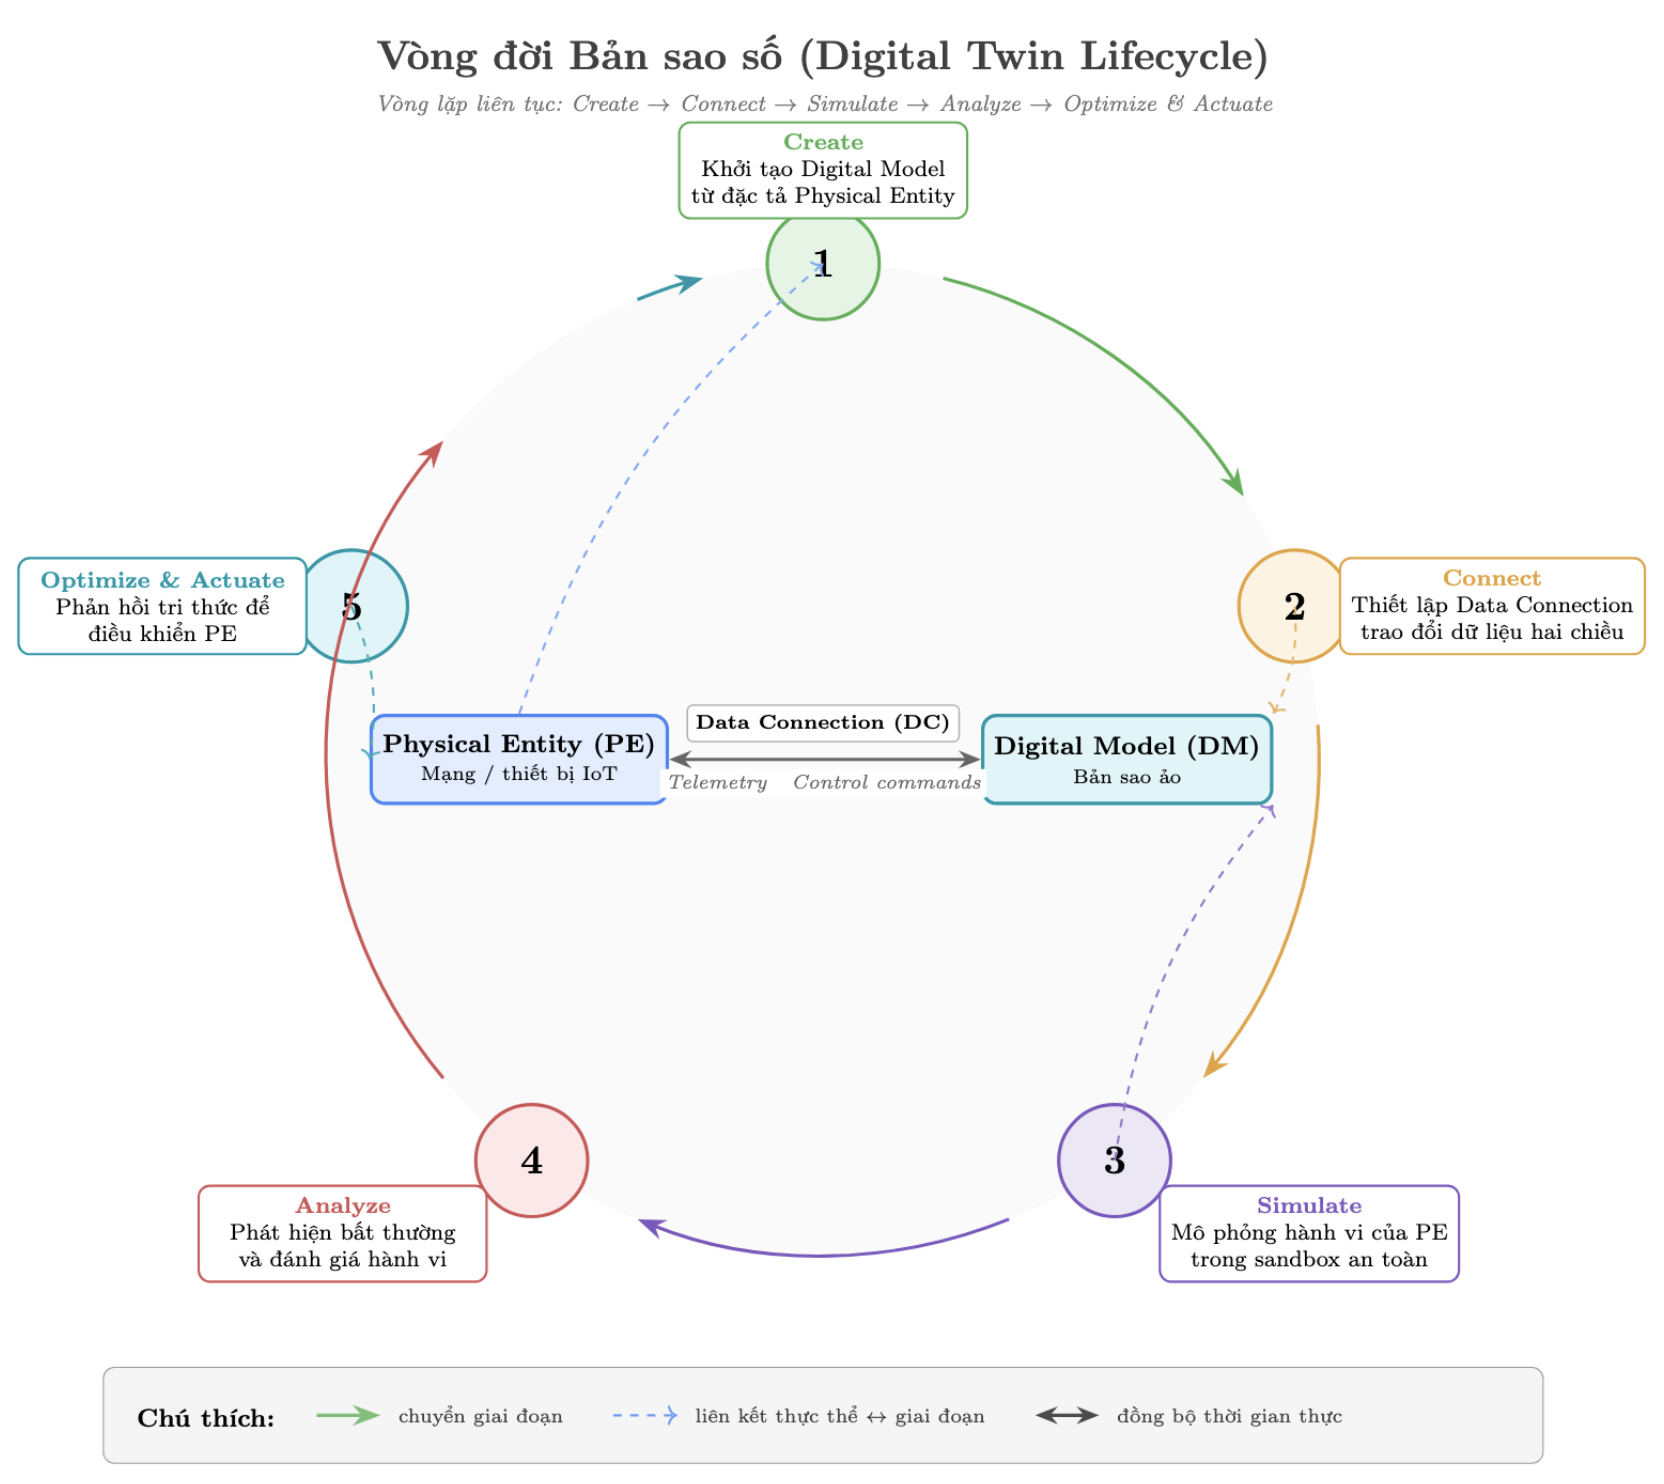
\includegraphics[width=0.85\linewidth]{Figures/fig_3_1_vong_doi_digital_twin.png}
    \caption{Vòng đời Digital Twin}
\end{figure}

Trong ngữ cảnh IoT, Digital Twin có nhiều ứng dụng như simulation (mô phỏng kịch bản khác nhau trên DT để dự báo hành vi trong tương lai hoặc kiểm thử chiến lược mới), optimization (tìm các tham số vận hành tối ưu cho thiết bị vật lý), anomaly detection (so sánh giữa trạng thái dự báo của DT và trạng thái thực tế của PE để phát hiện sai lệch), testing (kiểm thử hành vi hoặc chiến lược mới trong môi trường an toàn), và actuation (áp dụng các điều khiển hoặc hành động từ hệ thống kỹ thuật số về thiết bị vật lý).

\subsection{Server-side DT cho behavioral testing}
Trong DT-Guard, Digital Twin có chức năng khác biệt so với các ứng dụng DT truyền thống. Thay vì mirror một thiết bị vật lý cụ thể, Digital Twin trong DT-Guard là một môi trường kiểm thử (sandbox) tại server để chủ động kiểm chứng hành vi của từng mô hình cục bộ từ clients.

Sandbox isolation là một khía cạnh quan trọng của Digital Twin trong DT-Guard. Sandbox được tách biệt từ FL Server chính, có nghĩa là hành vi độc hại của một client không ảnh hưởng trực tiếp đến server hay các clients khác. Khi server nhận bản cập nhật từ một client, bản cập nhật này được triển khai vào sandbox để kiểm thử, không trực tiếp vào mô hình toàn cục. Sau khi kiểm thử xong, sandbox có thể được reset để chuẩn bị cho client tiếp theo.

Parallel verification là khả năng kiểm chứng song song nhiều clients. Mỗi sandbox có thể xử lý một client, và nhiều sandbox có thể chạy song song trên cùng một server hoặc trên nhiều server khác nhau. Điều này giúp giảm tổng thời gian verification khi số lượng clients lớn.

Challenge generation là khả năng sinh dữ liệu kiểm thử được kiểm soát. Digital Twin sử dụng bộ sinh dữ liệu thách thức (TabDDPM) để tạo ra dữ liệu kiểm thử có phân bổ nhãn cân bằng, bao phủ đa dạng các lớp tấn công, và phản ánh phân phối dữ liệu thực tế. Challenge data không phụ thuộc vào dữ liệu cục bộ của bất kỳ client nào, tạo ra một "sân chơi công bằng" để so sánh hành vi các clients.

\subsection{Kiểm chứng hành vi chủ động vs. Phân tích tham số thụ động}
Kiểm chứng hành vi chủ động (active behavioral verification) và phân tích tham số thụ động (passive parameter inspection) là hai paradigm khác nhau trong phòng thủ Federated Learning. Phân tích tham số thụ động chỉ quan sát tham số hoặc gradient, phát hiện bất thường qua metric thống kê (khoảng cách, norm, hướng dấu). Phương pháp này đơn giản nhưng có ba hạn chế: tham số không phản ánh trực tiếp hành vi suy luận; tấn công tối ưu ngược có thể giữ tham số trong vùng bình thường; và Non-IID khiến client lành tính dễ bị nhầm. Kiểm chứng hành vi chủ động đánh giá trực tiếp năng lực suy luận trên dữ liệu kiểm thử được kiểm soát, khắc phục cả ba hạn chế trên.

\section{Cơ sở lý thuyết mô hình sinh dữ liệu dạng bảng}
Chất lượng của challenge data ảnh hưởng trực tiếp đến độ tin cậy của toàn bộ pipeline kiểm định, do đó việc chọn được mô hình sinh phù hợp là yêu cầu tiên quyết. Với dữ liệu IDS dạng bảng (vừa có biến liên tục, vừa có biến phân loại, lại mất cân bằng nặng), không phải mô hình sinh nào cũng đáp ứng tốt. Đề tài khảo sát năm kiến trúc đại diện cho hai hướng tiếp cận khác nhau: nhóm Diffusion và nhóm GAN. Trước khi đi vào từng mô hình cụ thể, mục này nhắc lại nền tảng DDPM, vốn là gốc rễ chung của các biến thể diffusion được sử dụng trong luận văn.

\subsection{Denoising Diffusion Probabilistic Models (DDPM)}
Denoising Diffusion Probabilistic Models (DDPM) là nền tảng chung cho nhóm Diffusion, hoạt động theo hai quá trình: forward process (quá trình nhiễu dần) và reverse process (quá trình khử nhiễu dần).

Forward process là quá trình thêm nhiễu Gaussian vào dữ liệu ban đầu qua T bước. Có thể hình dung như việc nhỏ từ từ mực vào ly nước trong: mỗi bước thêm một lượng mực nhỏ, sau T bước nước hoàn toàn đen. Toán học, tại mỗi bước, dữ liệu được chuyển đổi bằng cách nhân với một hệ số giảm cộng thêm một lượng nhiễu Gaussian. Hệ số này được điều chỉnh theo lịch trình nhiễu đã định nghĩa trước, đảm bảo dữ liệu dần trở nên nhiễu theo cách có kiểm soát. Quá trình forward có đặc tính quan trọng: có thể tính trực tiếp dữ liệu tại bất kỳ bước t nào từ dữ liệu ban đầu, không cần tính qua tất cả các bước trung gian.

Reverse process là quá trình ngược lại, khôi phục dữ liệu từ nhiễu về dữ liệu ban đầu. Mô hình học một mạng neural network để dự đoán nhiễu tại từng bước, từ đó khôi phục dữ liệu bước trước. Trong quá trình huấn luyện, mô hình tối thiểu hóa sự khác biệt giữa nhiễu thực tế và nhiễu dự đoán, chia sẻ tham số giữa các bước. Trong quá trình sinh (inference), bắt đầu từ nhiễu ngẫu nhiên, lặp lại reverse process từ bước cuối về bước đầu để thu được dữ liệu mới.

\subsection{Nhóm Diffusion}
Nhóm Diffusion xây dựng trên nguyên lý khử nhiễu dần của DDPM, với các cải tiến chuyên biệt cho dữ liệu dạng bảng.

\textbf{TabDDPM: SOTA cho dữ liệu bảng} {[}7{]}

TabDDPM là biến thể của DDPM được thiết kế đặc biệt cho dữ liệu dạng bảng (tabular data): hỗn hợp biến liên tục và phân loại, không có cấu trúc lưới như ảnh, và thường có sự phụ thuộc phức tạp giữa các đặc trưng. TabDDPM có ba điểm khác biệt chính so với DDPM gốc: (1) xử lý song song biến liên tục bằng Gaussian diffusion và biến phân loại bằng multinomial diffusion; (2) kiến trúc mạng MLP với SiLU activation, residual connections, và attention mechanism (hidden layers 256 $\rightarrow$ 128 $\rightarrow$ 64); (3) hỗ trợ class-conditional generation bằng cách thêm thông tin nhãn vào đầu vào, cho phép sinh challenge data cân bằng nhãn, yêu cầu then chốt cho pipeline kiểm định của DT-Guard. TabDDPM đạt fidelity cao (TSTR cao), quá trình training ổn định (không gặp mode collapse như GAN), và hỗ trợ sinh theo nhãn chỉ định.

\textbf{TabSyn: Tối ưu luồng nhiễu dữ liệu hỗn hợp} {[}20{]}

TabSyn sử dụng VAE (Variational Autoencoder) kết hợp với diffusion trong latent space. Ý tưởng là trước tiên mã hóa dữ liệu vào không gian tiềm ẩn có chiều thấp hơn bằng VAE, sau đó huấn luyện mô hình diffusion trong không gian tiềm ẩn này để sinh latent vectors mới, cuối cùng giải mã về dữ liệu gốc. Cách tiếp cận này giảm chi phí tính toán nhưng phụ thuộc vào chất lượng của VAE mã hóa: nếu VAE không nắm bắt đầy đủ phân phối trong latent space, diffusion cũng không thể sinh ra mẫu chính xác.

\textbf{ForestDiffusion: Tích hợp thuật toán dạng cây} {[}6{]}

ForestDiffusion sử dụng Gradient Boosted Decision Trees (như XGBoost) thay vì mạng neural để khử nhiễu. Ở mỗi bước diffusion, ForestDiffusion huấn luyện một mô hình cây để dự đoán nhiễu. Ưu điểm là có thể chạy trên CPU mà không cần GPU, phù hợp cho môi trường tài nguyên hạn chế. Tuy nhiên, hạn chế là khả năng sinh đa dạng thấp hơn so với mô hình dựa trên neural network, và hỗ trợ conditional generation hạn chế.

\subsection{Nhóm GAN}
Nhóm GAN sử dụng cơ chế đối đầu (adversarial) giữa generator và discriminator, là paradigm phổ biến trước khi Diffusion xuất hiện.

\textbf{CTGAN: Chuyên biệt xử lý biến phân loại} {[}17{]}

CTGAN (Conditional Tabular GAN) sử dụng Conditional GAN để sinh dữ liệu bảng. CTGAN gồm hai mạng đối đầu: generator sinh dữ liệu giả từ nhiễu ngẫu nhiên, discriminator phân biệt giữa dữ liệu thật và giả, với điều kiện là giá trị của các biến phân loại. CTGAN xử lý đặc thù dữ liệu bảng bằng continuous embedding cho biến phân loại và mode-specific normalization cho biến liên tục. Hạn chế chính là mode collapse: generator có thể sinh ra một vài dạng mẫu lặp lại, không bao phủ toàn bộ phân phối thực.

\textbf{WGAN-GP: Mô hình đối sánh baseline} {[}4{]}

WGAN-GP (Wasserstein GAN with Gradient Penalty) là biến thể của GAN sử dụng Wasserstein distance thay vì Jensen-Shannon divergence làm hàm mất mát. Wasserstein distance cung cấp gradient mượt hơn, giúp quá trình huấn luyện ổn định hơn. Gradient penalty ràng buộc discriminator thỏa mãn điều kiện Lipschitz, giúp hội tụ tốt hơn. Tuy nhiên, WGAN-GP vẫn khó kiểm soát chất lượng sinh theo từng lớp (conditional generation) và có thể gặp mode collapse.

\subsection{Tiêu chí đánh giá và lựa chọn}
Năm mô hình trên được đánh giá qua A/B Testing (chi tiết tại Mục 5.3) trên bốn nhóm tiêu chí: Fidelity (TSTR, Wasserstein Distance), Coverage \& Diversity (Recall, DCR), Conditional Control (Label Accuracy), và Efficiency (Training Time). Kết quả cho thấy TabDDPM cân bằng tốt nhất giữa bốn tiêu chí và được chọn làm bộ sinh mặc định cho DT-Guard.

\section{Cơ sở lý thuyết mô hình Intrusion Detection}
DT-Guard cần một mô hình IDS đủ nhẹ để chạy được ở cả phía client (huấn luyện cục bộ) lẫn phía Digital Twin (chạy thử trên challenge data). IoTAttackNet, kiến trúc MLP được mô tả dưới đây, đáp ứng yêu cầu này; đi kèm là các chỉ số đánh giá được dùng xuyên suốt luận văn.

\subsection{Mô hình IoTAttackNet}
IoTAttackNet là một mạng MLP (Multilayer Perceptron) được thiết kế cho bài toán phân loại lưu lượng mạng IoT. MLP được chọn thay vì CNN hay RNN vì dữ liệu IDS dạng bảng không có cấu trúc không gian (như ảnh) hay tuần tự thời gian (như chuỗi), mỗi mẫu là một vector đặc trưng không gian phẳng, phù hợp với kiến trúc fully-connected. Kiến trúc chung là input $\rightarrow$ 256 $\rightarrow$ 128 $\rightarrow$ 64 $\rightarrow$ num\_classes (số lớp phân loại), với các thành phần sau:

Input layer: Nhận dữ liệu có d đặc trưng: với CIC-IoT-2023, d = 39 đặc trưng; với ToN-IoT, d = 10 đặc trưng.

Hidden layers: Ba lớp hidden với kích thước 256, 128, 64. Mỗi lớp sử dụng ReLU activation, BatchNorm để ổn định quá trình training, và Dropout với tỷ lệ 0,3 để ngăn overfitting.

Output layer: Lớp đầu ra có num\_classes neurons sử dụng Softmax activation để tạo phân phối xác suất trên các lớp: với CIC-IoT-2023, num\_classes = 34; với ToN-IoT, num\_classes = 10.

Hàm mất mát: Weighted Cross-Entropy Loss để xử lý mất cân bằng lớp.

Optimizer: Adam với learning rate = $10^{-3}$.

Việc sử dụng cùng kiến trúc MLP cho cả hai dataset cho phép đánh giá tính tổng quát hóa của DT-Guard một cách công bằng: nguyên lý kiểm chứng hành vi hoạt động hiệu quả bất kể số lượng đặc trưng (39 vs. 10) hay số lớp phân loại (34 vs. 10).

\subsection{Các chỉ số đánh giá}
Các chỉ số đánh giá được sử dụng trong DT-Guard bao gồm:

\textbf{(1) Accuracy}: tỷ lệ dự đoán đúng trên tổng số mẫu. Tính bằng tổng số mẫu được phân loại đúng chia cho tổng số mẫu. Accuracy cao cho thấy mô hình hoạt động tốt trên toàn bộ tập dữ liệu.

\textbf{(2) Precision}: tỷ lệ dự đoán đúng trong các mẫu được dự đoán là positive. Tính bằng số lượng positive được dự đoán đúng chia cho tổng số mẫu được dự đoán là positive. Precision cao nghĩa là khi mô hình dự đoán là positive, khả năng đúng là cao.

\textbf{(3) Recall (Detection Rate)}: tỷ lệ positive được phát hiện đúng. Tính bằng số lượng positive được dự đoán đúng chia cho tổng số positive thực tế. Recall cao nghĩa là mô hình phát hiện được hầu hết các positive.

\textbf{(4) F1-Score}: trung bình điều hòa của Precision và Recall. F1 cân bằng giữa hai chỉ số này, đặc biệt hữu ích khi có sự đánh đổi giữa Precision và Recall.

\[\text{F1} = \frac{2 \times \text{Precision} \times \text{Recall}}{\text{Precision} + \text{Recall}}\]

\textbf{(5) FPR (False Positive Rate)}: tỷ lệ negative bị dự đoán sai là positive. Tính bằng số lượng negative bị dự đoán là positive chia cho tổng số negative thực tế. FPR thấp nghĩa là mô hình ít khi đánh sai nhầm negative thành positive.

Trong ngữ cảnh DT-Guard, có hai tầng đánh giá cần phân biệt rõ: (1) Tầng 1 - FL defense: DT-Guard phát hiện client độc hại (Detection Rate, FPR ở cấp client); (2) Tầng 2 - IDS: Global model phát hiện tấn công mạng (Accuracy, F1 ở cấp traffic).

\section{Cơ sở lý thuyết bộ dữ liệu thực nghiệm}
Thực nghiệm trong luận văn sử dụng hai bộ dữ liệu IDS có quy mô và độ phức tạp khác nhau: CIC-IoT-2023 {[}11{]} (dataset gốc 46,7 triệu mẫu; thực nghiệm dùng slice Merged01.csv 712.311 mẫu, 39 đặc trưng, 34 lớp) và ToN-IoT {[}10{]} (461 nghìn mẫu, 10 đặc trưng, 10 lớp). Phần này giới thiệu nguồn gốc, cấu trúc đặc trưng và đặc điểm phân phối lớp tổng quan của từng bộ dữ liệu, cùng với cơ chế phân chia dữ liệu cho các client trong FL. Phân tích định lượng chi tiết (thống kê mô tả từng đặc trưng, biểu đồ phân phối, mức độ skew sau Dirichlet split) được trình bày tại Mục~5.1.6.

\subsection{CIC-IoT-2023}

\subsubsection{Tổng quan và cấu trúc đặc trưng}
CIC-IoT-2023 {[}11{]} được công bố bởi Canadian Institute for Cybersecurity năm 2023, thu thập từ hạ tầng 105 thiết bị IoT thực tế (camera, cảm biến, loa thông minh, v.v.) kết nối qua mạng có dây và không dây. Bộ dữ liệu gốc gồm 63 file CSV đã gộp (MERGED\_CSV); thực nghiệm trong luận văn sử dụng file Merged01.csv (147 MB, 712.311 mẫu) làm tập đại diện. Mỗi mẫu có 40 cột (39 đặc trưng mạng + 1 nhãn Label), được phân thành 5 nhóm (Bảng \ref{tab:cic_features}): thông tin header mạng (4), TCP flag (7), đếm flag (4), chỉ báo giao thức (15), và thống kê gói tin (9). Nhãn Label có 34 giá trị: BENIGN và 33 loại tấn công thuộc 7 danh mục (DDoS, DoS, Mirai, Spoofing, Reconnaissance, Web-based, BruteForce).

\begin{table}[H]
\centering
\caption{Phân nhóm 39 đặc trưng CIC-IoT-2023 {[}11{]}}
\label{tab:cic_features}
\small
\begin{tabular}{|l|c|p{7.5cm}|}
\hline
\textbf{Nhóm} & \textbf{SL} & \textbf{Các đặc trưng} \\
\hline
Thông tin header mạng & 4 & Header\_Length, Protocol Type, Time\_To\_Live, Rate \\
\hline
Cờ TCP (nhị phân) & 7 & fin\_flag\_number, syn\_flag\_number, rst\_flag\_number, psh\_flag\_number, ack\_flag\_number, ece\_flag\_number, cwr\_flag\_number \\
\hline
Số lượng cờ (0--100) & 4 & ack\_count, syn\_count, fin\_count, rst\_count \\
\hline
Chỉ báo giao thức (nhị phân) & 15 & HTTP, HTTPS, DNS, Telnet, SMTP, SSH, IRC, TCP, UDP, DHCP, ARP, ICMP, IGMP, IPv, LLC \\
\hline
Thống kê gói tin & 9 & Tot sum, Min, Max, AVG, Std, Tot size, IAT, Number, Variance \\
\hline
\end{tabular}
\end{table}

\subsubsection{Phân phối lớp tổng quan}
Dữ liệu CIC-IoT-2023 mất cân bằng cực kỳ nghiêm trọng: DDoS chiếm $\sim$72,8\% trong khi BruteForce chỉ chiếm $\sim$0,03\%, tỷ lệ chênh lệch khoảng 2.600$\times$. Phân phối chi tiết theo từng danh mục tấn công và đối chiếu với ToN-IoT được trình bày tại Mục~5.1.6.

\subsection{ToN-IoT}

\subsubsection{Tổng quan và cấu trúc đặc trưng}
ToN-IoT {[}10{]} được phát triển bởi Moustafa năm 2021 tại UNSW, thu thập từ kiến trúc Edge--Fog--Cloud sử dụng nền tảng SDN/NFV. Bộ dữ liệu cung cấp 44 đặc trưng mạng trích xuất bằng Zeek; DT-Guard sử dụng 10 đặc trưng quan trọng nhất sau feature selection, chuẩn hóa bằng StandardScaler.

\subsubsection{Phân phối lớp tổng quan}
ToN-IoT có dạng mất cân bằng \textit{one-vs-many}: lớp Normal chiếm $\sim$65\%, 8 lớp tấn công có khoảng 20.000 mẫu mỗi lớp, riêng MITM chỉ 1.042 mẫu. Bảng phân phối chi tiết và so sánh với CIC-IoT-2023 được trình bày tại Mục~5.1.6.

\subsection{Phân chia dữ liệu Federated bằng Dirichlet}
\label{sec:dirichlet_split}

Sau khi chia train--test (80/20, stratified), tập train được phân chia cho $N$ client bằng phân phối Dirichlet (Mục 3.1.3). Việc phân chia này tạo ra đồng thời ba dạng skew (\textit{quantity}, \textit{label}, \textit{feature}) đã định nghĩa ở Mục 3.1.3. Trong đó, client lành tính có dữ liệu bị skew nặng có thể phát sinh cập nhật ``lệch'' về mặt tham số, khiến các phương pháp phòng thủ thụ động (Krum, Median, Trimmed Mean) nhầm là độc hại---đây chính là Gap~2 mà DT-Guard giải quyết bằng kiểm chứng hành vi chủ động. Kết quả định lượng (mức độ skew nhãn theo từng client, phân phối giá trị đặc trưng theo client) được trình bày chi tiết tại Mục~5.1.6.

\subsection{So sánh và lựa chọn hai bộ dữ liệu}
Bảng \ref{tab:dataset_comparison} tóm tắt các đặc điểm khác biệt chính giữa hai bộ dữ liệu. Hai bộ dữ liệu này khác biệt rõ rệt về số đặc trưng (39 vs.\ 10) và số lớp (34 vs.\ 10), tạo điều kiện đánh giá khả năng tổng quát hóa của DT-Guard: nếu hệ thống hoạt động tốt trên cả hai, nguyên lý kiểm chứng hành vi là tổng quát, không phụ thuộc vào không gian đặc trưng cụ thể.

\begin{table}[H]
\centering
\caption{So sánh hai bộ dữ liệu thực nghiệm}
\label{tab:dataset_comparison}
\small
\begin{tabular}{|l|c|c|}
\hline
\textbf{Đặc điểm} & \textbf{CIC-IoT-2023} & \textbf{ToN-IoT} \\
\hline
Số mẫu (dataset gốc) & $\sim$46,7 triệu & $\sim$461 nghìn \\
\hline
Số mẫu (dùng trong thực nghiệm) & 712.311 (Merged01.csv) & 461.042 (toàn bộ) \\
\hline
Số đặc trưng (sử dụng) & 39 & 10 \\
\hline
Số lớp & 34 & 10 \\
\hline
Lớp đa số / thiểu số & DDoS 72,82\% / BruteForce 0,03\% & Normal 65\% / MITM 0,23\% \\
\hline
Tỷ lệ chênh lệch max/min & $\sim$2.600$\times$ & $\sim$288$\times$ \\
\hline
\end{tabular}
\end{table}

\section{Tổng kết chương}
Chương này đã trình bày cơ sở lý thuyết cho sáu thành phần chính: Federated Learning, các tấn công poisoning/backdoor, Digital Twin, mô hình sinh dữ liệu dạng bảng, mô hình Intrusion Detection, và bộ dữ liệu thực nghiệm. Hai bộ dữ liệu CIC-IoT-2023 và ToN-IoT có ba đặc điểm quan trọng: (1) mất cân bằng lớp nghiêm trọng (tỷ lệ chênh lệch 288--2.600$\times$); (2) dữ liệu có đặc tính Non-IID khi phân chia Dirichlet, đặc biệt với $\alpha=0{,}1$; (3) sự khác biệt rõ rệt về số đặc trưng (39 vs.\ 10) và số lớp (34 vs.\ 10) giúp đánh giá tính tổng quát hóa của hệ thống. Các lý thuyết này tạo cơ sở cho Chương~4, nơi trình bày kiến trúc hệ thống DT-Guard để giải quyết ba khoảng trống nghiên cứu đã nhận diện.

% Chapter 4
\chapter{ĐỀ XUẤT HỆ THỐNG DT-GUARD}
\label{Chapter4}

Chương này mô tả kiến trúc DT-Guard, khung phòng thủ chủ động cho FL trong IoT IDS. Nội dung gồm: phát biểu bài toán, kiến trúc tổng thể, bộ sinh dữ liệu thách thức, pipeline kiểm định 4 lớp, cơ chế DT-PW với Effort Gate, và phân tích lý thuyết.

\section{Phát biểu bài toán và ý tưởng cốt lõi}

\subsection{Phát biểu bài toán phòng thủ trong FL-IDS}
Xét hệ thống FL-IDS gồm N client $\{C_{1}, C_{2}, \ldots, C_{N}\}$ cùng huấn luyện một mô hình phát hiện xâm nhập toàn cục $\mathbf{w}$ qua R vòng lặp. Trong đó, tập client bao gồm N - K client lành tính (tập B) và K client độc hại (tập M), với K không biết trước. Mỗi client i sở hữu tập dữ liệu cục bộ $D_{i}$ có phân phối Non-IID theo Dirichlet($\alpha)$.

Bài toán phòng thủ được phát biểu:

\textbf{Đầu vào:} Tại mỗi round t, server nhận tập bản cập nhật $\{\mathbf{w}_{1}^{(t)}, \mathbf{w}_{2}^{(t)}, \ldots, \mathbf{w}_{N}^{(t)}\}$ từ N client. Server có quyền truy cập mô hình toàn cục $\mathbf{w}^{(t-1)}$ của round trước nhưng không có quyền truy cập dữ liệu thô $D_{i}$ của bất kỳ client nào.

\textbf{Đầu ra mong muốn:} (1) Mô hình toàn cục $\mathbf{w}^{(t)}$ duy trì Accuracy cao bất chấp sự hiện diện của tập M; (2) Phát hiện và loại bỏ chính xác client thuộc M: Detection Rate (DR) cao, False Positive Rate (FPR) thấp; (3) Trọng số tổng hợp $w_{i}$ phản ánh đúng mức đóng góp tri thức thực tế, gán $w_{i}$ = 0 cho free-rider.

\textbf{Ràng buộc:} (1) Không truy cập dữ liệu thô, server chỉ thấy tham số mô hình; (2) Overhead tính toán phải nhỏ hơn 1\% tổng thời gian mỗi round; (3) Hoạt động hiệu quả trên nhiều loại tấn công (Backdoor, LIE, Min-Max, Min-Sum, MPAF) và nhiều tỉ lệ K/N (10\%--50\%).

\subsection{Ý tưởng cốt lõi: Kiểm chứng hành vi chủ động}
Như đã phân tích trong Chương 2, nguyên nhân gốc rễ của ba khoảng trống nghiên cứu nằm ở cách tiếp cận phân tích tham số thụ động: tất cả các phương pháp phòng thủ hiện có đều chỉ phân tích đặc trưng tĩnh của tham số mô hình mà không kiểm chứng hành vi suy luận thực tế.

DT-Guard đề xuất chuyển từ \textbf{passive parameter inspection} sang \textbf{active behavioral verification}: thay vì chỉ đánh giá hình thái tham số, server chủ động kiểm chứng năng lực suy luận của mô hình trên dữ liệu kiểm thử được kiểm soát. Cách tiếp cận này dựa trên hai \textbf{giả thuyết khoa học} sau:

\textbf{Giả thuyết H1 (Client Non-IID lành tính):} Client i $\in$ B có dữ liệu $D_{i}$ thiên lệch về một số lớp sẽ có tham số $\mathbf{w}_{i}$ lệch xa mô hình toàn cục $\mathbf{w}$. Các phương pháp thụ động (Krum, GeoMed, LUP) đo $\|\mathbf{w}_{i} - \mathbf{w}\|_{2}$ và dễ nhầm đây là tấn công, gây FPR cao. Tuy nhiên, khi được kiểm tra trên dữ liệu thách thức cân bằng nhãn $D_{\text{ch}}$, mô hình vẫn phân loại chính xác, vì client đã thực sự học được tri thức hữu ích từ dữ liệu riêng.

\textbf{Giả thuyết H2 (Tấn công tối ưu ngược):} Client j $\in$ M sử dụng LIE {[}1{]}, Min-Max/Min-Sum {[}15{]} có thể giữ $\mathbf{w}_{j}$ trong vùng phân phối thống kê bình thường ($\|\mathbf{w}_{j} - \mathbf{w}\|_{2}$ nhỏ), khiến các phương pháp thụ động không phát hiện được. Tuy nhiên, khi buộc phải phân loại trên $D_{\text{ch}}$, mô hình sẽ bộc lộ hành vi sai: F1 thấp trên các lớp tấn công.

Digital Twin đóng vai trò môi trường kiểm thử cách ly (sandbox) tại phía server để thực hiện kiểm chứng này một cách an toàn và tách biệt. Cách tiếp cận này cho phép server kiểm chứng từng mô hình trước khi chấp nhận, thay vì chỉ suy luận từ tham số.

\subsection{Ký hiệu toán học}

\begin{longtable}[]{@{}
  >{\raggedright\arraybackslash}p{(\linewidth - 2\tabcolsep) * \real{0.1547}}
  >{\raggedright\arraybackslash}p{(\linewidth - 2\tabcolsep) * \real{0.7733}}@{}}
\caption{Bảng tổng hợp các ký hiệu toán học chính} \\
\toprule\noalign{}
\begin{minipage}[b]{\linewidth}\centering
\textbf{Ký hiệu}
\end{minipage} & \begin{minipage}[b]{\linewidth}\centering
\textbf{Ý nghĩa}
\end{minipage} \\
\midrule\noalign{}
\endfirsthead
%
\multicolumn{2}{c}{{\textit{(tiếp) Bảng 4.1}}} \\
\toprule\noalign{}
\begin{minipage}[b]{\linewidth}\centering
\textbf{Ký hiệu}
\end{minipage} & \begin{minipage}[b]{\linewidth}\centering
\textbf{Ý nghĩa}
\end{minipage} \\
\midrule\noalign{}
\endhead
\bottomrule\noalign{}
\endlastfoot
N & Số client tổng cộng \\
K & Số client độc hại \\
$\mathbf{w}^{(t)}$ & Tham số mô hình toàn cục tại round t \\
$\mathbf{w}_{i}^{(t)}$ & Tham số mô hình cục bộ của client i tại round t \\
$D_{\text{ch}}$ & Bộ dữ liệu thách thức (challenge data) \\
M & Số mẫu trong $D_{\text{ch}}$ \\
L & Số lớp (layer) trainable trong mô hình \\
$s_{i}(ids)$ & IDS Performance Score của client i \\
$s_{i}(param)$ & Parameter Similarity Score của client i \\
$\Delta_{i}^{(t)}$ & Mức lệch tham số chuẩn hóa của client i \\
$T_{i}$ & Trust-Score tổng hợp của client i \\
$d_{i}$ & Prediction divergence của client i \\
$P_{i}$ & Performance-Score của client i \\
$w_{i}$ & Trọng số tổng hợp cuối cùng của client i \\
A & Tập client được chấp nhận (qua cả Trust Gate và Effort Gate) \\
\end{longtable}

\section{Kiến trúc tổng thể DT-Guard}

\subsection{Kiến trúc ba thực thể}
DT-Guard được thiết kế với ba thực thể chính, tách biệt về chức năng và vị trí triển khai:

\textbf{IoT Clients (Tầng cạnh):} Các thiết bị IoT hoặc edge node thực hiện huấn luyện cục bộ trên dữ liệu riêng $D_{i}$ và gửi bản cập nhật $\mathbf{w}_{i}^{(t)}$ về server. Mỗi client sử dụng optimizer Adam với learning rate = $10^{-3}$, batch size 512, huấn luyện E = 3 local epoch mỗi round. Loss function là Weighted Cross-Entropy để xử lý mất cân bằng lớp. Trong thiết lập thực nghiệm, hệ thống gồm 20 client với phân bổ dữ liệu Non-IID theo Dirichlet ($\alpha$ = 0,5).

\textbf{FL Server (Tầng trung tâm):} Server trung tâm điều phối toàn bộ quy trình FL. Server nhận bản cập nhật từ client, chuyển tiếp sang DT Verification Environment để kiểm chứng, nhận kết quả Trust-Score và Performance-Score, thực hiện tổng hợp mô hình toàn cục, và phân phối lại cho client. Server lưu trữ mô hình toàn cục $\mathbf{w}^{(t)}$ và lịch sử kiểm chứng của từng client.

\textbf{DT Verification Environment (Tầng kiểm chứng):} Môi trường kiểm chứng Digital Twin, được tách biệt khỏi FL Server chính. Việc tách biệt cung cấp ba lợi ích: (1) Cách ly hành vi độc hại: mô hình độc hại chạy trong sandbox không ảnh hưởng đến vòng lặp FL chính, vì sandbox sử dụng bản sao tham số và tài nguyên riêng; (2) Kiểm chứng song song: server có thể khởi tạo nhiều DT instance để kiểm tra nhiều client đồng thời, giúp giảm tổng thời gian verification khi số client lớn; (3) Tách biệt verification khỏi aggregation: quy trình kiểm chứng không ảnh hưởng đến thread tổng hợp chính, giữ cho server luôn responsive.

Hình 4.1 trình bày kiến trúc tổng quát của DT-Guard với ba thực thể và luồng tương tác giữa chúng. Ở cấp độ tổng quát, mỗi vòng FL diễn ra như sau: các client gửi bản cập nhật lên FL Server (1); server chuyển tiếp sang DT Verification Environment để kiểm chứng (2); bản cập nhật đạt chuẩn được tổng hợp (3), mô hình toàn cục mới được trả về server (4) và phân phối lại cho client (5). Toàn bộ logic đánh giá (từ sinh dữ liệu thách thức, kiểm định hành vi, đến chấm điểm đóng góp) đều nằm bên trong DT Verification Environment.

\begin{figure}[H]
    \centering
    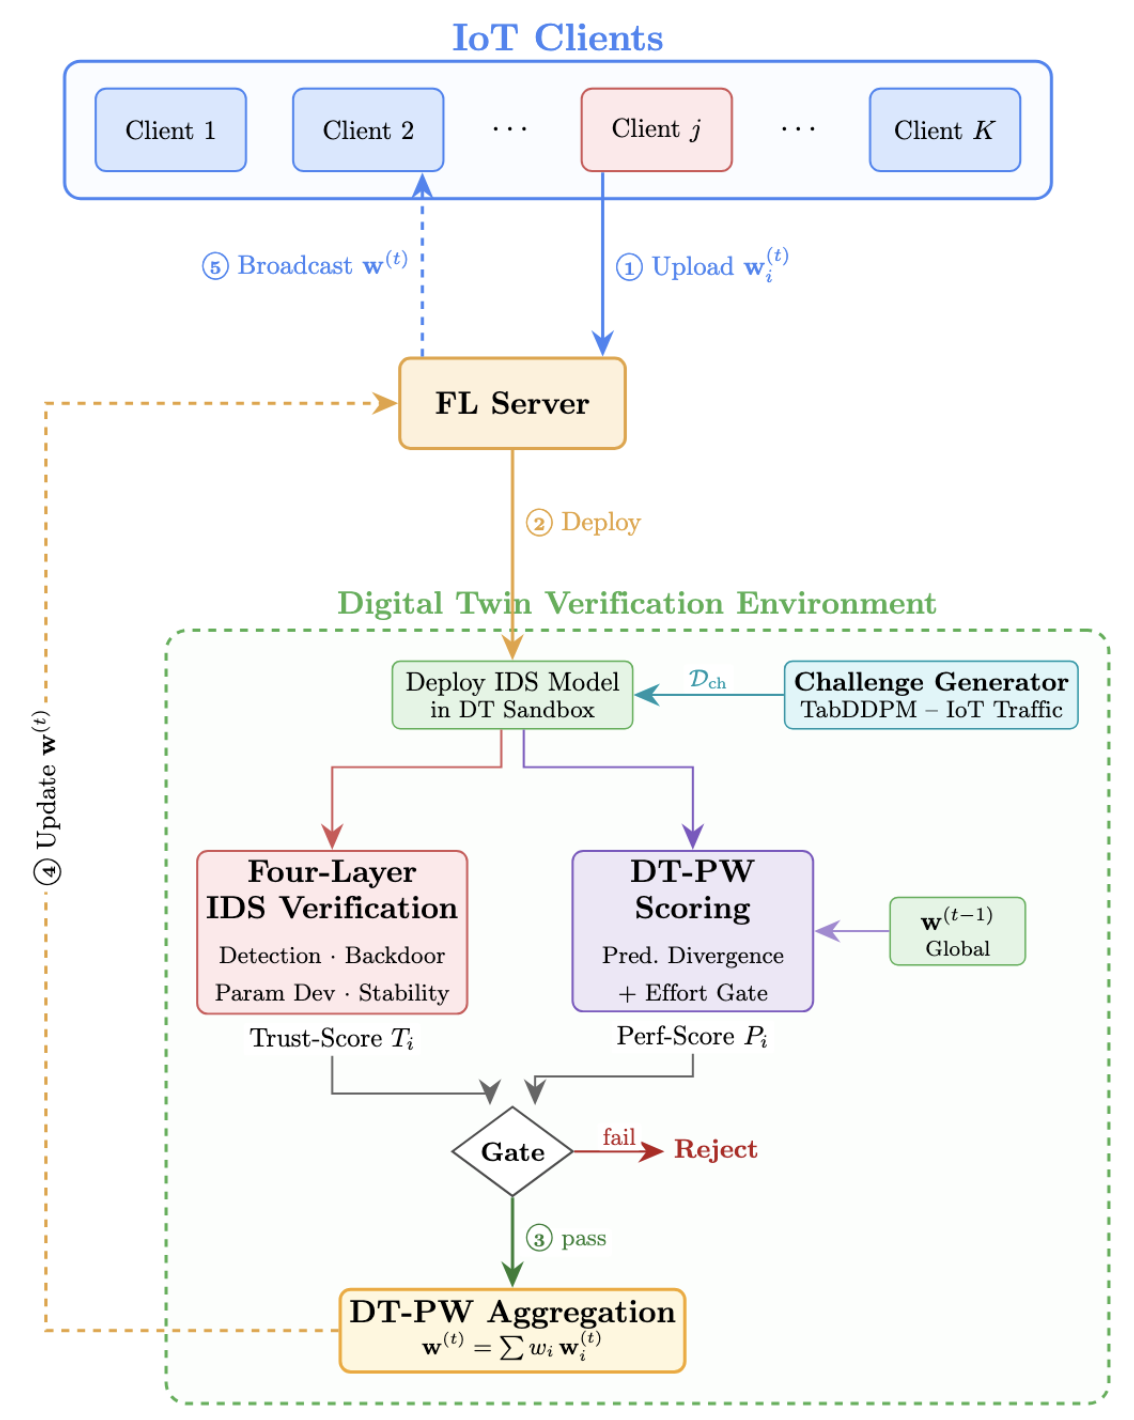
\includegraphics[width=0.85\linewidth]{Figures/fig_4_1_kien_truc_tong_quat_dtguard.png}
    \caption{Kiến trúc tổng quát DT-Guard}
\end{figure}

Phần tiếp theo sẽ đi sâu vào bên trong DT Verification Environment, thành phần cốt lõi tạo nên sự khác biệt của DT-Guard so với các phương pháp hiện có.

\subsection{Cấu trúc bên trong DT Verification Environment}
\begin{figure}[H]
    \centering
    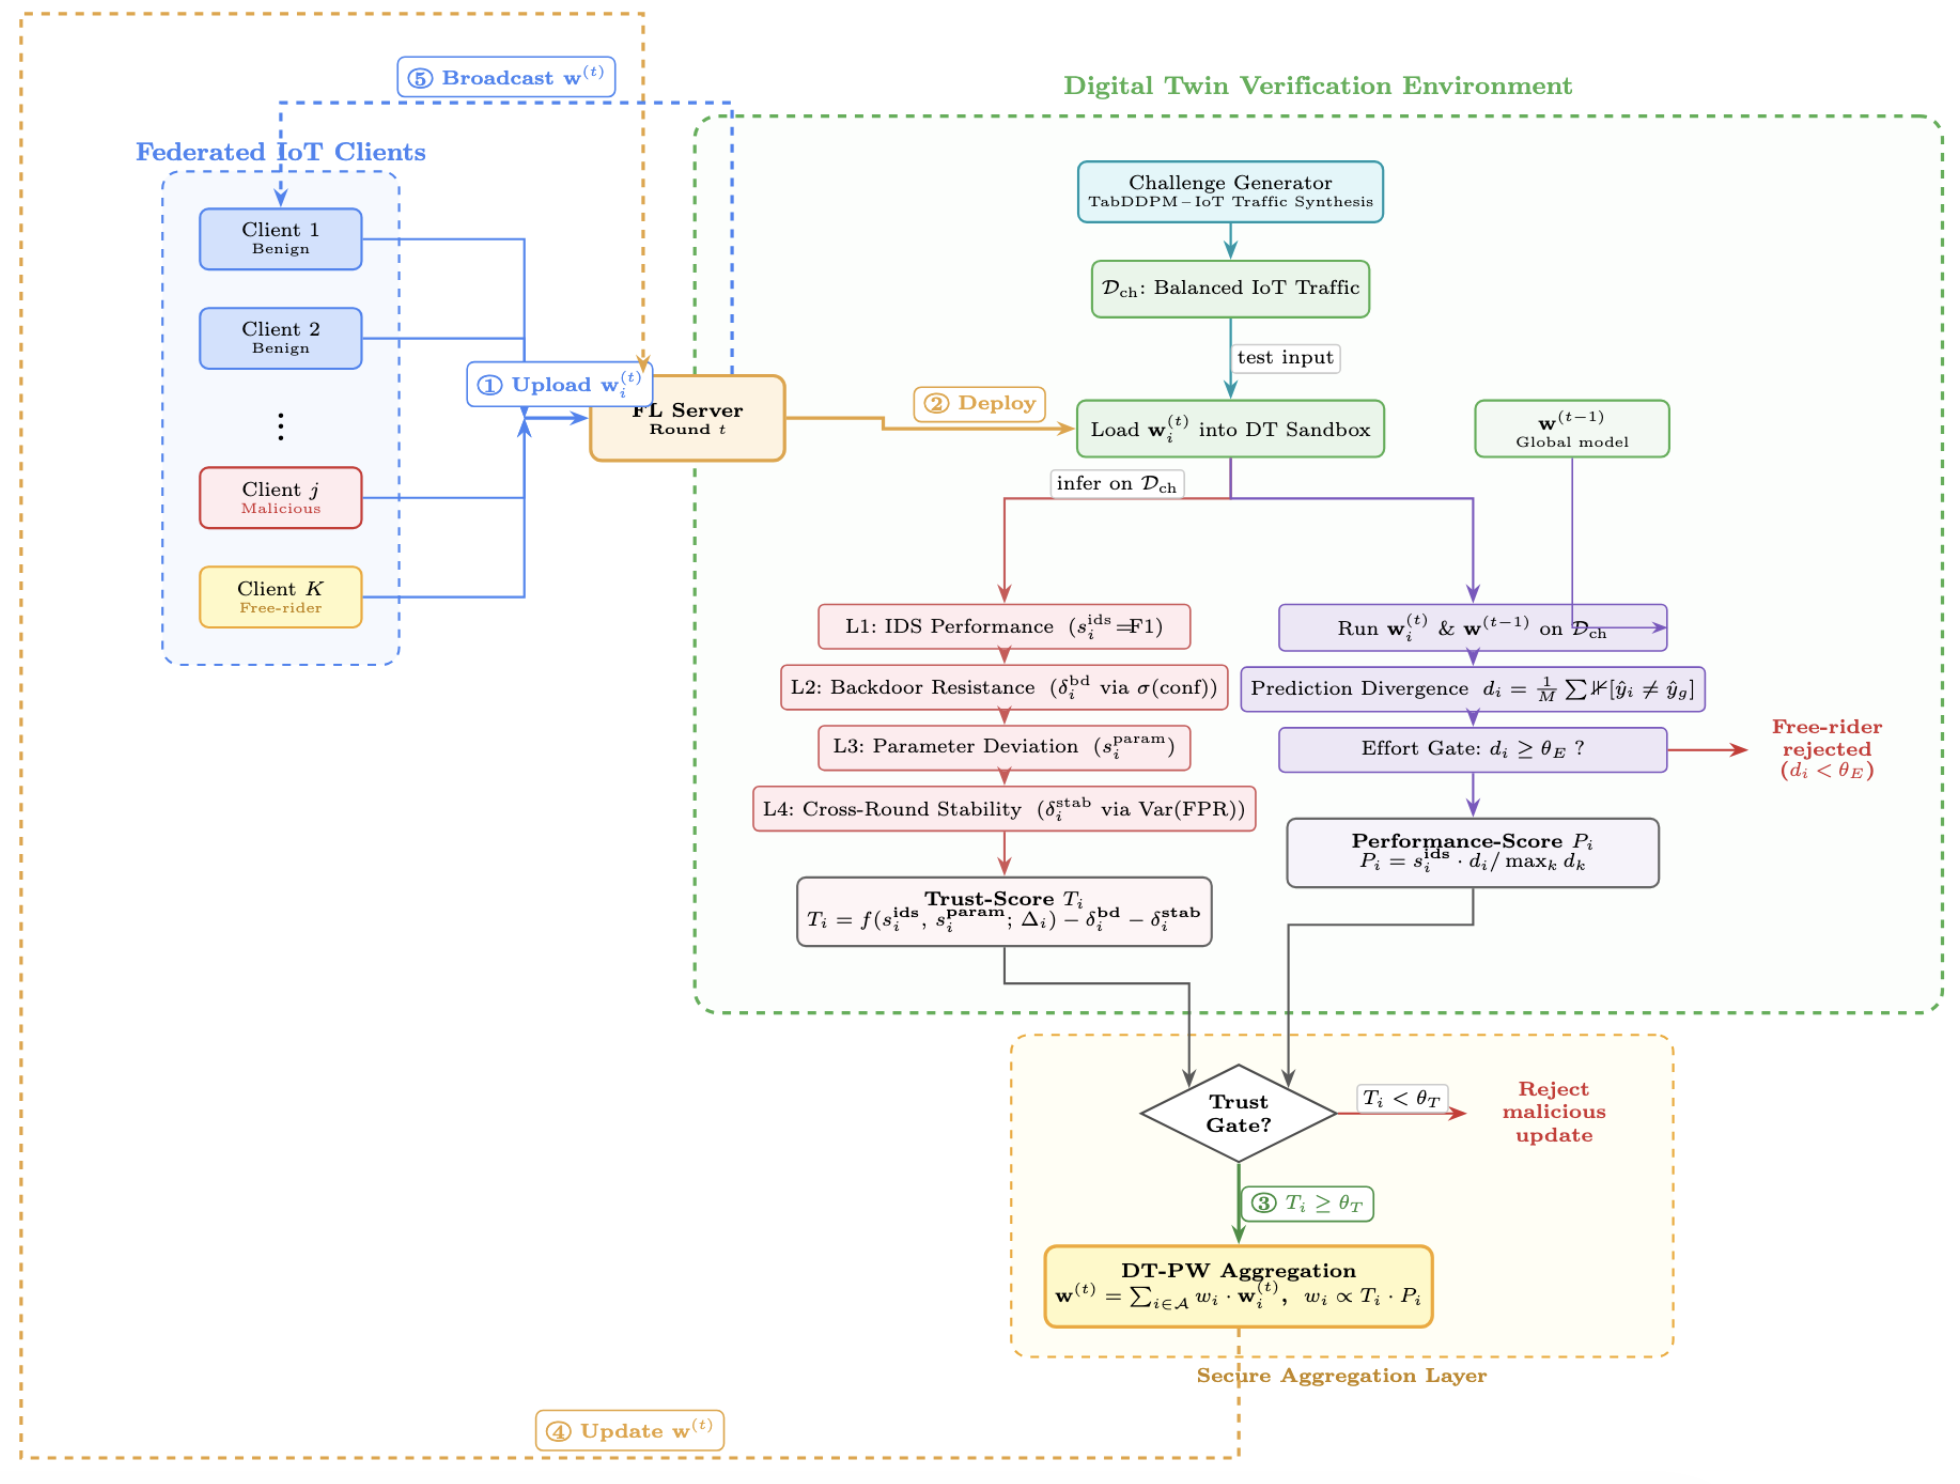
\includegraphics[width=0.85\linewidth]{Figures/fig_4_2_kien_truc_dt_verification_environment.png}
    \caption{Kiến trúc chi tiết DT Verification Environment}
\end{figure}

DT Verification Environment được tổ chức thành bốn tầng xử lý nối tiếp nhau. Mỗi bản cập nhật $\mathbf{w}_{i}^{(t)}$ từ client đi qua lần lượt các tầng này trước khi được chấp nhận hoặc loại bỏ.

Tầng sinh dữ liệu: Challenge Generator. Đây là tầng trên cùng, chịu trách nhiệm cung cấp dữ liệu kiểm thử cho toàn bộ quy trình phía dưới. Challenge Generator sử dụng TabDDPM {[}7{]} để sinh tập $D_{\text{ch}}$ (bao gồm cả lưu lượng bình thường lẫn nhiều dạng tấn công) khác nhau, với phân bổ nhãn cân bằng. Dữ liệu này đóng vai trò "đề thi" mà mọi mô hình cục bộ phải vượt qua. $D_{\text{ch}}$ được sinh trước và lưu sẵn (pre-generated pool), nên không tạo thêm độ trễ trong mỗi vòng FL.

Tầng cách ly: DT Sandbox. Khi FL Server chuyển một bản cập nhật $\mathbf{w}_{i}^{(t)}$ sang DT Environment, bản cập nhật này được nạp vào một sandbox tách biệt. Sandbox chỉ làm việc với bản sao tham số, không sử dụng tham số gốc; mỗi lần chỉ nạp một mô hình rồi giải phóng trước khi nạp mô hình tiếp theo; và được reset về trạng thái sạch sau mỗi lần kiểm chứng. Thiết kế này đảm bảo mô hình độc hại không thể ảnh hưởng đến server hay các mô hình khác.

Từ sandbox, quá trình đánh giá phân thành hai nhánh song song, mỗi nhánh giải quyết một bài toán riêng biệt:

Nhánh thứ nhất: Four-Layer Verification Pipeline. Nhánh này trả lời câu hỏi: \emph{"Mô hình này có đáng tin hay không?"} Mô hình được chạy trên $D_{\text{ch}}$ rồi đánh giá qua bốn lớp kiểm định liên tiếp: (L1) hiệu năng phát hiện xâm nhập, (L2) khả năng kháng backdoor, (L3) mức lệch tham số so với mô hình toàn cục, và (L4) độ ổn định hành vi qua các vòng. Bốn điểm thành phần được tổng hợp thành một Trust-Score $T_{i}$ duy nhất. Chi tiết từng lớp được trình bày tại Mục 4.4.

Nhánh thứ hai: DT-PW Scoring. Nhánh này trả lời câu hỏi: \emph{"Mô hình này có đóng góp tri thức mới hay không?"} Cả mô hình cục bộ $\mathbf{w}_{i}^{(t)}$ lẫn mô hình toàn cục $\mathbf{w}^{(t-1)}$ đều được chạy trên cùng $D_{\text{ch}}$, rồi so sánh kết quả dự đoán của chúng. Mức khác biệt trong dự đoán (gọi là prediction divergence $d_{i})$ phản ánh lượng tri thức mới mà client mang lại. Nếu $d_{i}$ quá thấp (dự đoán gần như trùng khớp với mô hình toàn cục), Effort Gate xác định đó là free-rider và gán điểm đóng góp bằng không. Client vượt qua Effort Gate được chấm Performance-Score $P_{i}$. Chi tiết được trình bày tại Mục 4.5.

Tầng quyết định (Decision Gate). Kết quả từ hai nhánh (Trust-Score $T_{i}$ và Performance-Score $P_{i})$ hội tụ tại đây. Tầng này thực hiện hai bước lọc tuần tự: trước hết, client có $T_{i}$ dưới ngưỡng tin cậy $\theta_{T}$ bị loại bỏ (bản cập nhật bị từ chối); tiếp theo, trong số các client còn lại, những client đã bị Effort Gate đánh dấu là free-rider ($P_{i}$ = 0) cũng bị gán trọng số bằng không. Tập client cuối cùng vượt qua cả hai bộ lọc gọi là $\mathcal{A}$.

Tầng tổng hợp (DT-PW Aggregator). Chỉ các bản cập nhật thuộc tập $\mathcal{A}$ mới tham gia vào việc tổng hợp mô hình toàn cục mới. Trọng số của mỗi client được tính bằng tích $T_{i}$ $\cdot$ $P_{i}$ (chuẩn hóa), đảm bảo client nào vừa đáng tin vừa đóng góp nhiều tri thức mới sẽ có ảnh hưởng lớn nhất. Mô hình toàn cục mới $\mathbf{w}^{(t)}$ sau đó được chuyển ngược lại FL Server.

\subsection{Lý do thiết kế hai nhánh song song}
Việc tách quá trình đánh giá thành hai nhánh độc lập xuất phát từ nhận định rằng hai bài toán (phát hiện client độc hại và phát hiện free-rider) có bản chất khác nhau và không thể giải bằng cùng một chỉ số.

Client độc hại cố tình phá hoại mô hình toàn cục, nhưng có thể ngụy trang tham số để trông bình thường. Để phát hiện chúng, cần đánh giá hành vi suy luận thực tế trên nhiều khía cạnh: đó là việc của Four-Layer Pipeline.

Free-rider không phá hoại, nhưng cũng không đóng góp gì: chúng chỉ sao chép mô hình toàn cục rồi gửi lại. Mô hình của free-rider vẫn phân loại đúng (vì bản chất là mô hình toàn cục), nên Four-Layer Pipeline không loại được chúng. Để phát hiện free-rider, cần so sánh dự đoán cục bộ với dự đoán toàn cục: đó là việc của DT-PW Scoring.

Hai nhánh sử dụng chung $D_{\text{ch}}$ làm đầu vào nhưng tính toán độc lập. Trust-Score đánh giá chất lượng tuyệt đối của mô hình, Performance-Score đánh giá mức đóng góp tương đối so với mô hình toàn cục. Chỉ khi kết hợp cả hai qua Công thức (4.11), hệ thống mới đồng thời loại được client độc hại, loại free-rider, và ưu tiên client đóng góp thực chất.

\subsection{Luồng hoạt động 5 bước mỗi vòng FL}
Mỗi vòng FL \emph{t} diễn ra theo năm bước:

\textbf{Bước 1 (Upload).} Mỗi client i nhận mô hình toàn cục $\mathbf{w}^{(t-1)}$ từ server, huấn luyện cục bộ E = 3 epoch trên dữ liệu riêng $D_{i}$ (optimizer Adam, lr = $10^{-3}$, batch size 512, Weighted Cross-Entropy loss), và gửi bản cập nhật $\mathbf{w}_{i}^{(t)}$ về FL Server. Tại thời điểm này, server chưa có thông tin nào về độ tin cậy hay mức đóng góp của từng client.

\textbf{Bước 2 (Deploy).} Thay vì tổng hợp ngay, FL Server chuyển từng $\mathbf{w}_{i}^{(t)}$ sang DT Verification Environment. Mô hình được nạp vào sandbox và chạy inference trên $D_{\text{ch}}$. Hai nhánh đánh giá hoạt động tuần tự: Four-Layer Pipeline tính Trust-Score $T_{i}$; DT-PW Scorer tính prediction divergence $d_{i}$ và Performance-Score $P_{i}$.

\textbf{Bước 3 (Gate \& Aggregate).} Decision Gate kiểm tra hai điều kiện: (a) Trust Gate: nếu $T_{i}$ \textless $\theta_{T}$, bản cập nhật bị từ chối ($\theta_{T}$ = 0,6 cho CIC-IoT-2023, $\theta_{T}$ = 0,5 cho ToN-IoT, được điều chỉnh theo độ phức tạp của từng dataset); (b) Effort Gate: trong số các client còn lại, nếu $d_{i}$ \textless $\theta_{E}$ thì $P_{i}$ = 0 (free-rider). Tập client cuối cùng được chấp nhận là $\mathcal{A}$.

\textbf{Bước 4 (Update).} Mô hình toàn cục mới được tổng hợp: $\mathbf{w}^{(t)}$ = $\sum_{i \in \mathcal{A}} w_{i} \cdot \mathbf{w}_{i}^{(t)}$ với trọng số:

\[w_{i} = \frac{T_{i} \cdot P_{i}}{\sum_{k \in \mathcal{A}}^{}(T_{k} \cdot P_{k})}\]

Kết quả được chuyển ngược lại FL Server.

\textbf{Bước 5 (Broadcast).} FL Server phân phối $\mathbf{w}^{(t)}$ cho tất cả N client để bắt đầu vòng lặp tiếp theo.

\section{Bộ sinh dữ liệu thách thức (Challenge Data Generator)}

\subsection{Vai trò và yêu cầu}
Trong hệ thống FL-IDS, server không có quyền truy cập dữ liệu thô của client. Do đó, để kiểm chứng hành vi mô hình, server cần một bộ sinh dữ liệu (generative model) để tạo ra dữ liệu kiểm thử đại diện, gọi là challenge data $D_{\text{ch}}$. Chất lượng của $D_{\text{ch}}$ quyết định trực tiếp khả năng phân biệt của toàn bộ khung DT-Guard.

$D_{\text{ch}}$ cần đáp ứng bốn yêu cầu:

\textbf{(1) Fidelity (Độ trung thực):} Phân phối dữ liệu tổng hợp phải gần với phân phối dữ liệu thực, đo bằng TSTR (Train on Synthetic, Test on Real), khoảng cách Wasserstein (biến liên tục), và Jensen-Shannon Distance (biến phân loại).

\textbf{(2) Coverage \& Diversity (Bao phủ và đa dạng):} Dữ liệu phải bao phủ đa dạng các lớp lưu lượng, đồng thời các mẫu sinh ra phải đa dạng, tránh mode collapse, đo bằng DCR (Distance to Closest Record) và hệ chỉ số PRDC (Precision, Recall, Density, Coverage).

\textbf{(3) Conditional Control (Kiểm soát điều kiện):} Bộ sinh phải hỗ trợ class-conditional generation (sinh mẫu theo nhãn chỉ định) để tạo $D_{\text{ch}}$ cân bằng nhãn. Đo bằng Label Accuracy qua Oracle classifier.

\textbf{(4) Efficiency (Hiệu quả):} Tốc độ huấn luyện và sinh mẫu phải đủ nhanh để tích hợp vào vòng lặp FL mà không tạo nút thắt, đo bằng Training Time, Generation Latency, và CPU/RAM.

\subsection{A/B Testing chọn mô hình sinh}
Đề tài tiến hành A/B Testing trên năm mô hình sinh dữ liệu dạng bảng thuộc hai họ:

\begin{itemize}
\item
  \textbf{Nhóm Diffusion:} TabDDPM {[}7{]}: MLP denoising, 256 hidden units, SiLU activation, \emph{T} = 200 bước, 100 epoch; TabSyn {[}20{]}: VAE kết hợp latent diffusion, 256 hidden units; ForestDiffusion {[}6{]}: sử dụng XGBoost thay vì neural network để khử nhiễu, chỉ chạy trên CPU.
\item
  \textbf{Nhóm GAN:} CTGAN {[}17{]}: Conditional GAN chuyên biệt dữ liệu bảng, mode-specific normalization, 256 hidden units, 300 epoch; WGAN-GP {[}4{]}: Wasserstein GAN với gradient penalty $\lambda$ = 10, 256 hidden units, 300 epoch.
\end{itemize}

\textbf{Quy trình A/B Testing gồm ba bước:}

\textbf{(Bước 1) Huấn luyện và sinh dữ liệu.} Mỗi mô hình được huấn luyện trên cùng tập dữ liệu seed (một phần dữ liệu mà server nắm giữ, không chứa dữ liệu cục bộ của bất kỳ client nào), đảm bảo điều kiện đầu vào đồng nhất cho so sánh công bằng. Sau khi huấn luyện, mỗi mô hình sinh cùng số lượng mẫu với phân bổ nhãn cân bằng giữa các lớp, tạo ra năm tập dữ liệu tổng hợp $\{\hat{D}_{1}, \hat{D}_{2}, \ldots, \hat{D}_{5}\}$.

\textbf{(Bước 2) Đánh giá theo bốn nhóm tiêu chí.} Mỗi tập dữ liệu tổng hợp $\hat{D}_{i}$ được đánh giá trên cả CIC-IoT-2023 và ToN-IoT qua bốn nhóm tiêu chí:

\begin{itemize}
\item
  \textbf{Fidelity}: dữ liệu tổng hợp phản ánh sát phân phối thực tế đến mức nào. Đo bằng hai chỉ số: TSTR (Train on Synthetic, Test on Real), huấn luyện mô hình phân loại trên $\hat{D}_{i},$ kiểm tra trên dữ liệu thật; TSTR càng cao thì dữ liệu sinh càng sát thực. Wasserstein Distance: khoảng cách giữa phân phối đặc trưng của $\hat{D}_{i}$ và dữ liệu thật; giá trị càng thấp càng tốt.
\item
  \textbf{Coverage \& Diversity}: dữ liệu bao phủ đầy đủ và đa dạng các lớp lưu lượng hay không. Đo bằng Recall (tỷ lệ mẫu thật có ít nhất một mẫu sinh gần tương tự, Recall cao nghĩa là không bỏ sót vùng nào của phân phối thực) và DCR (Distance to Closest Record, khoảng cách từ mẫu sinh đến mẫu thật gần nhất, đảm bảo không trùng lặp).
\item
  \textbf{Conditional Control}: bộ sinh có tạo được mẫu theo nhãn chỉ định chính xác không. Đo bằng Label Accuracy qua Oracle classifier, huấn luyện một mô hình phân loại trên dữ liệu thật, dùng nó kiểm tra nhãn của mẫu sinh; accuracy cao nghĩa là conditional generation hoạt động tốt.
\item
  \textbf{Efficiency}: chi phí tính toán để huấn luyện và sinh mẫu. Đo bằng Training Time (thời gian huấn luyện) và Generation Latency (thời gian sinh một batch).
\end{itemize}

\textbf{(Bước 3) Tổng hợp composite score và lựa chọn.} Bốn nhóm tiêu chí được chuẩn hóa về thang {[}0, 10{]} rồi tổng hợp thành composite score có trọng số bằng nhau. TabDDPM đạt composite score cao nhất (7,3/10) nhờ: TSTR 71,4\% (cao nhất); Wasserstein Distance 0,061 (thấp nhất); Recall 0,98 (gần bao phủ toàn bộ); Training time \textasciitilde200 giây (nhanh gấp $8\times$ CTGAN). Kết quả nhất quán trên cả hai dataset. Chi tiết kết quả A/B Testing tại Mục 5.3.

\subsection{Quy trình sinh dữ liệu thách thức}
Quy trình sinh $D_{\text{ch}}$ được thiết kế để tối ưu hóa giữa chất lượng kiểm thử và chi phí tính toán, gồm ba giai đoạn:

\textbf{(Giai đoạn 1)} Huấn luyện TabDDPM trên dữ liệu seed (thực hiện một lần trước vòng lặp FL): Server sử dụng tập dữ liệu seed (một phần dữ liệu công khai hoặc dữ liệu mà server nắm giữ, \textbf{không} chứa dữ liệu cục bộ của bất kỳ client nào) để huấn luyện mô hình TabDDPM. Cấu hình huấn luyện: kiến trúc MLP với 256 hidden units, activation SiLU, \emph{T} = 200 bước diffusion, 100 epoch. Biến liên tục được xử lý bằng Gaussian diffusion, biến phân loại bằng multinomial diffusion (chi tiết tại Mục 3.4.2). Quá trình huấn luyện mất khoảng 200 giây trên CIC-IoT-2023 và nhanh hơn trên ToN-IoT nhờ không gian đặc trưng nhỏ hơn. Thời điểm huấn luyện được thực hiện trước khi bắt đầu vòng lặp FL, nên không ảnh hưởng đến thời gian mỗi round.

\textbf{(Giai đoạn 2)} Sinh trước challenge pool (pre-generation): Sau khi huấn luyện, TabDDPM sử dụng khả năng class-conditional generation để sinh trước một pool \emph{P} gồm hàng nghìn mẫu với phân bổ nhãn cân bằng (mỗi lớp \emph{C} có số mẫu tương đương, với CIC-IoT-2023, \emph{C} = 34 lớp; với ToN-IoT, \emph{C} = 10 lớp). Việc cân bằng nhãn là then chốt vì: nếu challenge data thiếu một lớp tấn công cụ thể (ví dụ: Backdoor), pipeline sẽ không thể phát hiện client đầu độc nhắm vào lớp đó. Pool \emph{P} được lưu trên đĩa (persistent storage) để tái sử dụng qua nhiều round, loại bỏ hoàn toàn latency sinh dữ liệu trong vòng lặp FL. Pool được refresh khi cần (ví dụ khi phân phối dữ liệu thay đổi đáng kể do concept drift) bằng cách tái huấn luyện TabDDPM trên dữ liệu seed mới.

\textbf{(Giai đoạn 3)} Lấy mẫu mỗi round (sampling): Tại mỗi round \emph{t}, một batch $D_{\text{ch}}$ gồm M mẫu được lấy ngẫu nhiên từ pool \emph{P}, với ràng buộc cân bằng nhãn: mỗi lớp góp mặt ít nhất $\lfloor M/C \rfloor$ mẫu. Giá trị M được thiết lập theo đặc thù dataset: M = 200 cho CIC-IoT-2023 (34 lớp, không gian 39 chiều) và M = 500 cho ToN-IoT (10 lớp, không gian 10 chiều). M nhỏ hơn trên CIC-IoT-2023 vì chi phí inference tăng theo số đặc trưng, nhưng vẫn đủ để đánh giá đáng tin cậy (thực nghiệm cho thấy M = 200 cho kết quả ổn định). Mỗi round sử dụng một batch khác nhau từ pool, đảm bảo đa dạng dữ liệu kiểm thử. Nếu pool cạn kiệt hoặc cần mẫu mới, TabDDPM sinh thêm bằng conditional sampling mà không cần tái huấn luyện.

\textbf{Tại sao quy trình này hiệu quả:} Ba giai đoạn tách bạch mang lại lợi ích quan trọng. Giai đoạn 1 và 2 diễn ra offline trước vòng lặp FL, nên không tạo thêm độ trễ. Giai đoạn 3 chỉ là thao tác lấy mẫu từ pool đã có sẵn (O(M) rất nhanh). Kết quả thực nghiệm cho thấy toàn bộ overhead sinh challenge data mỗi round là không đáng kể so với thời gian huấn luyện cục bộ (chi tiết tại Mục 5.5).

\section{Pipeline kiểm định hành vi với Trust-Score}
Pipeline kiểm định hành vi 4 lớp là thành phần cốt lõi của DT-Guard, giải quyết Khoảng trống 1 (phòng thủ trước đa dạng tấn công) và Khoảng trống 2 (phân biệt Non-IID với đầu độc). Pipeline được kiểm soát bởi các tham số: $\alpha$ $\in$ {[}0, 1{]} cân bằng hiệu năng IDS và tương đồng tham số; $\lambda_{\text{bd}}$, $\lambda_{\text{stab}}$ $\in$ $\mathbb{R}^{+}$ là hệ số phạt; $D_{\max}$ \textgreater 0 chuẩn hóa khoảng cách tham số; $\theta_{\text{div}}$ \textgreater 0 là ngưỡng chuyển sang strict mode; $\theta_{T}$ $\in$ {[}0, 1{]} là ngưỡng chấp nhận.

\begin{figure}[H]
    \centering
    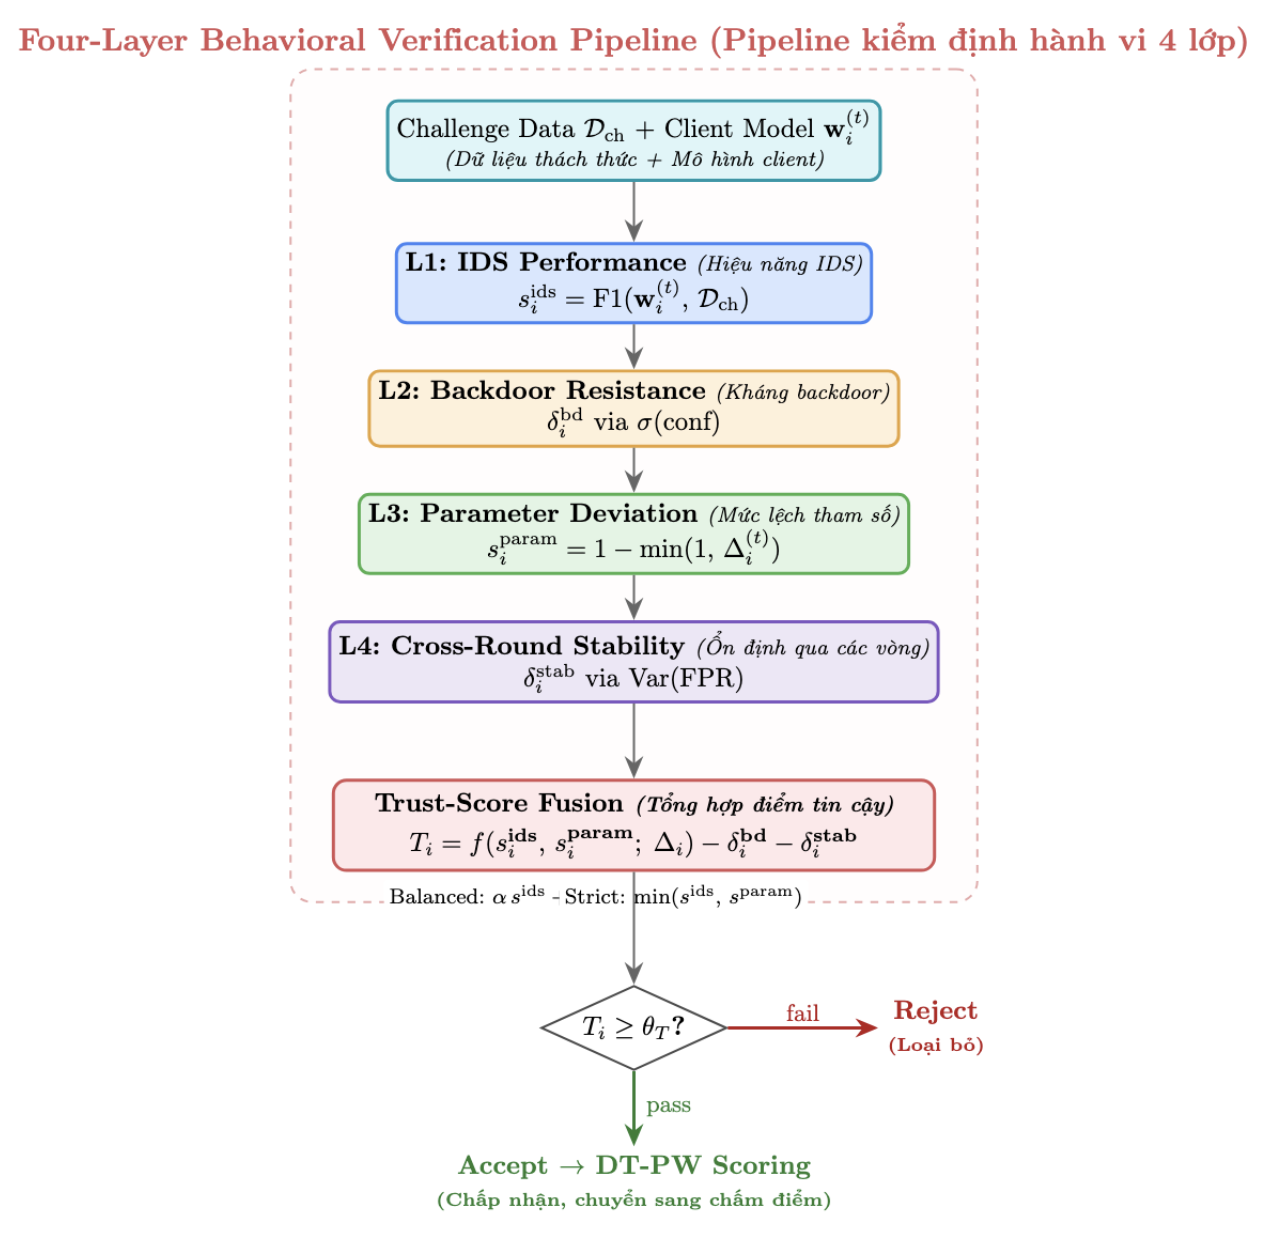
\includegraphics[width=0.85\linewidth]{Figures/fig_4_3_pipeline_kiem_dinh_4_lop.png}
    \caption{Pipeline kiểm định hành vi 4 lớp với Trust-Score}
\end{figure}

\subsection{Lớp 1: IDS Performance Score}
Lớp đầu tiên đánh giá trực tiếp năng lực phát hiện xâm nhập của mô hình cục bộ trên dữ liệu thách thức. Mô hình $\mathbf{w}_{i}^{(t)}$ được nạp vào sandbox, chạy inference trên toàn bộ $D_{\text{ch}}$, và được chấm điểm bằng F1-Score (phân loại nhị phân benign vs. attack):

\begin{equation}
s_{i}(\text{ids}) = F1(\mathbf{w}_{i}^{(t)},D_{\text{ch}}) \in \lbrack 0,1\rbrack
\tag{4.1}
\end{equation}

Trong đó: $s_{i}(ids)$ là IDS Performance Score của client i; F1($\cdot,\cdot)$ là F1-Score phân loại nhị phân (benign vs. attack); $\mathbf{w}_{i}^{(t)}$ là tham số mô hình cục bộ của client i tại round t; $D_{\text{ch}}$ là bộ dữ liệu thách thức gồm M mẫu.

F1-Score được chọn thay vì Accuracy vì cân bằng giữa Precision và Recall, phù hợp cho bài toán mất cân bằng lớp trong IDS. Mô hình lành tính (dù tham số lệch do Non-IID) vẫn đạt F1 cao vì đã thực sự học tri thức IDS hữu ích. Mô hình bị đầu độc có F1 thấp do phân loại sai trên các lớp tấn công mà nó bị nhắm đến.

Đây là lớp quan trọng nhất trong pipeline vì đánh giá trực tiếp năng lực suy luận của mô hình thay vì chỉ xem xét tham số. Các tấn công như LIE hay Min-Max có thể giữ tham số trong vùng bình thường, nhưng khi phải phân loại trên $D_{\text{ch}}$, hiệu năng thực tế sẽ suy giảm rõ rệt, kéo $s_{i}(ids)$ xuống thấp. Ngược lại, client Non-IID lành tính có tham số lệch nhưng vẫn phân loại chính xác, nên $s_{i}(ids)$ vẫn cao.

\subsection{Lớp 2: Backdoor Resistance Score}
Lớp thứ hai nhắm đến tấn công backdoor, loại tấn công khó phát hiện nhất vì mô hình hoạt động bình thường trên dữ liệu sạch, chỉ sai khi gặp trigger. DT-Guard khai thác quan sát: mô hình nhiễm backdoor có phân phối confidence bất thường, khi gặp mẫu gần trigger, softmax confidence lệch mạnh so với bình thường.

Cụ thể, DT-Guard tính độ lệch chuẩn $\sigma(conf)$ của softmax confidence trên $D_{\text{ch}}$. Nếu $\sigma(conf)$ vượt ngưỡng $\tau_{\text{bd}}$ (ước lượng từ mô hình toàn cục làm chuẩn), mô hình bị phạt:

\begin{equation}
\delta_{i}(\text{bd}) = \begin{cases}
  \lambda_{\text{bd}} & \text{nếu }\sigma(\text{conf}(\mathbf{w}_{i}^{(t)},D_{\text{ch}})) > \tau_{\text{bd}} \\
  0 & \text{nếu ngược lại}
\end{cases}\
\tag{4.2}
\end{equation}

Trong đó: $\delta_{i}(bd)$ là Backdoor Penalty của client i; $\sigma(\cdot)$ là độ lệch chuẩn của softmax confidence trên $D_{\text{ch}}$; $\tau_{\text{bd}}$ là ngưỡng variance confidence (ước lượng từ mô hình toàn cục); $\lambda_{\text{bd}}$ là hệ số phạt. Mô hình sạch có confidence ổn định nên không bị phạt. Mô hình nhiễm backdoor có confidence dao động mạnh khi gặp các mẫu gần trigger nên bị phạt $\lambda_{\text{bd}}$.

Cách tiếp cận này không cần biết trước trigger pattern, điều không khả thi trong FL vì server không có quyền truy cập dữ liệu của client. Thay vào đó, DT-Guard phát hiện gián tiếp thông qua dấu hiệu bất thường trong phân phối confidence. Mô hình nhiễm backdoor phải duy trì đồng thời hai hành vi đối lập (phân loại đúng trên dữ liệu sạch và phân loại sai khi có trigger), điều này tạo ra phân phối confidence không tự nhiên mà lớp kiểm định này có thể nắm bắt.

\subsection{Lớp 3: Parameter Deviation Score}
Lớp thứ ba đánh giá mức lệch tham số của mô hình cục bộ so với mô hình toàn cục. DT-Guard tính trung bình khoảng cách L2 theo từng lớp (layer) của mô hình, chuẩn hóa bằng $D_{\max}$:

\begin{equation}
\Delta_{i}^{(t)} = \frac{1}{L} \cdot \sum_{l = 1}^{L}\frac{\left\| \mathbf{w}_{i,l}^{(t)} - \mathbf{w}_{l}^{\left( t-1 \right)} \right\|_{2}}{D_{\max}} \geq 0
\tag{4.3}
\end{equation}

Trong đó: $\Delta_{i}^{(t)}$ là mức lệch tham số chuẩn hóa của client i tại round t; L là số lớp (layer) trainable trong mô hình; $\mathbf{w}_{i,l}^{(t)}$ là tham số lớp $\ell$ của client i; $\mathbf{w}_{l}^{(t-1)}$ là tham số lớp $\ell$ của mô hình toàn cục round trước; $D_{\max}$ \textgreater 0 là hằng số chuẩn hóa. Giá trị $\Delta_{i}$ được ánh xạ sang điểm tương đồng:

\begin{equation}
s_{i}(\text{param}) = 1 - \min(1,\Delta_{i}^{(t)}) \in \lbrack 0,1\rbrack
\tag{4.4}
\end{equation}

Trong đó $s_{i}(param)$ là Parameter Similarity Score. Khi $\Delta_{i}$ \textgreater 1, tham số lệch vượt giới hạn chuẩn hóa, $s_{i}(param)$ = 0.

Cần lưu ý rằng lớp này không được sử dụng đơn lẻ để quyết định chấp nhận hay loại bỏ client, vì làm vậy sẽ gây FPR cao giống như Krum, GeoMed hay LUP. Thay vào đó, Parameter Deviation đóng vai trò thông tin bổ sung cho cơ chế fusion thích ứng ở Mục 4.4.5. Khi $\Delta_{i}$ cao, hệ thống tự động chuyển sang strict mode, đồng thời yêu cầu $s_{i}(ids)$ cũng phải đạt mức cao. Nhờ vậy, DT-Guard phân biệt được client Non-IID lành tính ($\Delta_{i}$ cao nhưng $s_{i}(ids)$ cao vì phân loại đúng) với client độc hại ($\Delta_{i}$ cao và $s_{i}(ids)$ thấp vì phân loại sai).

\subsection{Lớp 4: Cross-Round Stability Score}
Lớp thứ tư phát hiện hành vi bất ổn định qua các vòng, dấu hiệu của attacker thay đổi chiến thuật liên tục hoặc mô hình bị nhiễu ngẫu nhiên. DT-Guard theo dõi FPR (False Positive Rate ở cấp traffic) của mỗi client qua cửa sổ trượt $\tau$ round gần nhất. Nếu variance vượt ngưỡng $\tau_{\text{stab}}$, client bị phạt:

\begin{equation}
\delta_{i}(\text{stab}) = \begin{cases}
  \lambda_{\text{stab}} & \text{nếu Var}(FPR_{i}^{\left( t-\tau \right)},\ldots,FPR_{i}^{(t)}) > \tau_{\text{stab}} \\
  0 & \text{nếu ngược lại}
\end{cases}\
\tag{4.5}
\end{equation}

Trong đó: $\delta_{i}(stab)$ là Stability Penalty của client i; Var($\cdot)$ là phương sai; $FPR_{i}^{(t)}$ là False Positive Rate ở cấp traffic của client i tại round t; $\tau$ là kích thước cửa sổ trượt; $\tau_{\text{stab}}$ là ngưỡng variance FPR; $\lambda_{\text{stab}}$ là hệ số phạt. Client mới (chưa đủ $\tau$ round lịch sử) được gán $\delta_{i}(stab)$ = 0 (không phạt).

Lớp này dựa trên quan sát rằng client lành tính có hành vi ổn định qua các round: FPR thay đổi ít. Trong khi đó, attacker thường thay đổi chiến thuật qua các vòng (ví dụ round trước sử dụng LIE, round sau chuyển sang Min-Max), tạo ra biến động lớn trong FPR và bị lớp kiểm định này phát hiện.

\subsection{Trust-Score Fusion}
Bốn lớp được tổng hợp thành Trust-Score duy nhất $T_{i}$ qua cơ chế fusion thích ứng. Trust-Score bao gồm điểm cơ bản trừ đi hai penalty:

\begin{equation}
T_{i} = f(s_{i}(\text{ids}),s_{i}(\text{param});\Delta_{i}^{(t)}) - \delta_{i}(\text{bd}) - \delta_{i}(\text{stab})
\tag{4.6}
\end{equation}

Trong đó hàm \emph{f}($\cdot)$ tổng hợp Lớp 1 và Lớp 3 theo cơ chế thích ứng hai chế độ dựa trên mức lệch tham số:

\[f( \cdot ) = \alpha \cdot s_{i}(\text{ids}) + (1 - \alpha) \cdot s_{i}(\text{param})\text{nếu }\Delta_{i}^{(t)} \leq \theta_{\text{div}}\text{(balanced mode)(4.7a)}\]

\[f( \cdot ) = \min(s_{i}(\text{ids}),s_{i}(\text{param}))\text{nếu }\Delta_{i}^{(t)} > \theta_{\text{div}}\text{(strict mode)(4.7b)}\]

Trong đó: $\alpha$ $\in$ {[}0, 1{]} là trọng số cân bằng giữa hiệu năng IDS và tương đồng tham số; $\theta_{\text{div}}$ \textgreater 0 là ngưỡng chuyển chế độ.

Balanced mode ($\Delta_{i}$ $\leq$ $\theta_{\text{div}}$): Tham số lệch ít, khả năng cao là client bình thường. Hệ thống sử dụng kết hợp tuyến tính với $\alpha$ = 0,7, ưu tiên IDS Performance (đánh giá hành vi trực tiếp) hơn Parameter Similarity (thông tin gián tiếp). Chế độ này cho phép client Non-IID có $s_{i}(param)$ trung bình nhưng $s_{i}(ids)$ cao vẫn đạt Trust-Score tốt.

Strict mode ($\Delta_{i}$ \textgreater $\theta_{\text{div}}$): Tham số lệch nhiều, cần kiểm tra nghiêm ngặt. Hệ thống lấy min: cả $s_{i}(ids)$ và $s_{i}(param)$ phải đồng thời cao. Client độc hại dù giữ $s_{i}(param)$ trung bình (qua tối ưu ngược) nhưng $s_{i}(ids)$ thấp $\rightarrow$ min thấp $\rightarrow$ bị loại. Client Non-IID lành tính có $\Delta_{i}$ cao nhưng $s_{i}(ids)$ cũng cao (phân loại đúng trên challenge data) $\rightarrow$ min vẫn đủ cao.

Sau khi tính $T_{i},$ client chỉ được chấp nhận khi $T_{i}$ $\geq$ $\theta_{T}$ ($\theta_{T}$ = 0,6 cho CIC-IoT-2023, $\theta_{T}$ = 0,5 cho ToN-IoT). Tập client vượt qua Trust Gate gọi là $\mathcal{T}$.

\begin{longtable}[]{@{}
  >{\raggedright\arraybackslash}p{(\linewidth - 4\tabcolsep) * \real{0.1474}}
  >{\raggedright\arraybackslash}p{(\linewidth - 4\tabcolsep) * \real{0.3669}}
  >{\raggedright\arraybackslash}p{(\linewidth - 4\tabcolsep) * \real{0.4857}}@{}}
\caption{Bảng tổng hợp tham số Trust Gate} \\
\toprule\noalign{}
\begin{minipage}[b]{\linewidth}\centering
\textbf{Tham số}
\end{minipage} & \begin{minipage}[b]{\linewidth}\centering
\textbf{Giá trị}
\end{minipage} & \begin{minipage}[b]{\linewidth}\centering
\textbf{Ý nghĩa}
\end{minipage} \\
\midrule\noalign{}
\endfirsthead
%
\multicolumn{3}{c}{{\textit{(tiếp) Bảng 4.2}}} \\
\toprule\noalign{}
\begin{minipage}[b]{\linewidth}\centering
\textbf{Tham số}
\end{minipage} & \begin{minipage}[b]{\linewidth}\centering
\textbf{Giá trị}
\end{minipage} & \begin{minipage}[b]{\linewidth}\centering
\textbf{Ý nghĩa}
\end{minipage} \\
\midrule\noalign{}
\endhead
\bottomrule\noalign{}
\endlastfoot
$\alpha$ & 0,7 & Tỉ trọng IDS Performance trong balanced mode \\
$\theta_{\text{div}}$ & Tùy chỉnh & Ngưỡng chuyển balanced $\rightarrow$ strict mode \\
$\lambda_{\text{bd}}$ & Tùy chỉnh & Hệ số phạt backdoor \\
$\lambda_{\text{stab}}$ & Tùy chỉnh & Hệ số phạt bất ổn định \\
$\theta_{T}$ & 0,6 (CIC-IoT-2023) / 0,5 (ToN-IoT) & Ngưỡng chấp nhận Trust-Score \\
$D_{\max}$ & 0 & Hằng số chuẩn hóa khoảng cách tham số \\
\end{longtable}

\section{Cơ chế DT-PW với Effort Gate}
Cơ chế DT-Driven Performance Weighting (DT-PW) giải quyết Khoảng trống 3: thiếu cơ chế đo đóng góp tri thức thực tế và vấn đề free-rider. Sau khi client vượt qua Trust Gate (tập $\mathcal{T}),$ DT-PW tiếp tục đánh giá mức đóng góp tri thức mới của từng client.

\begin{figure}[H]
    \centering
    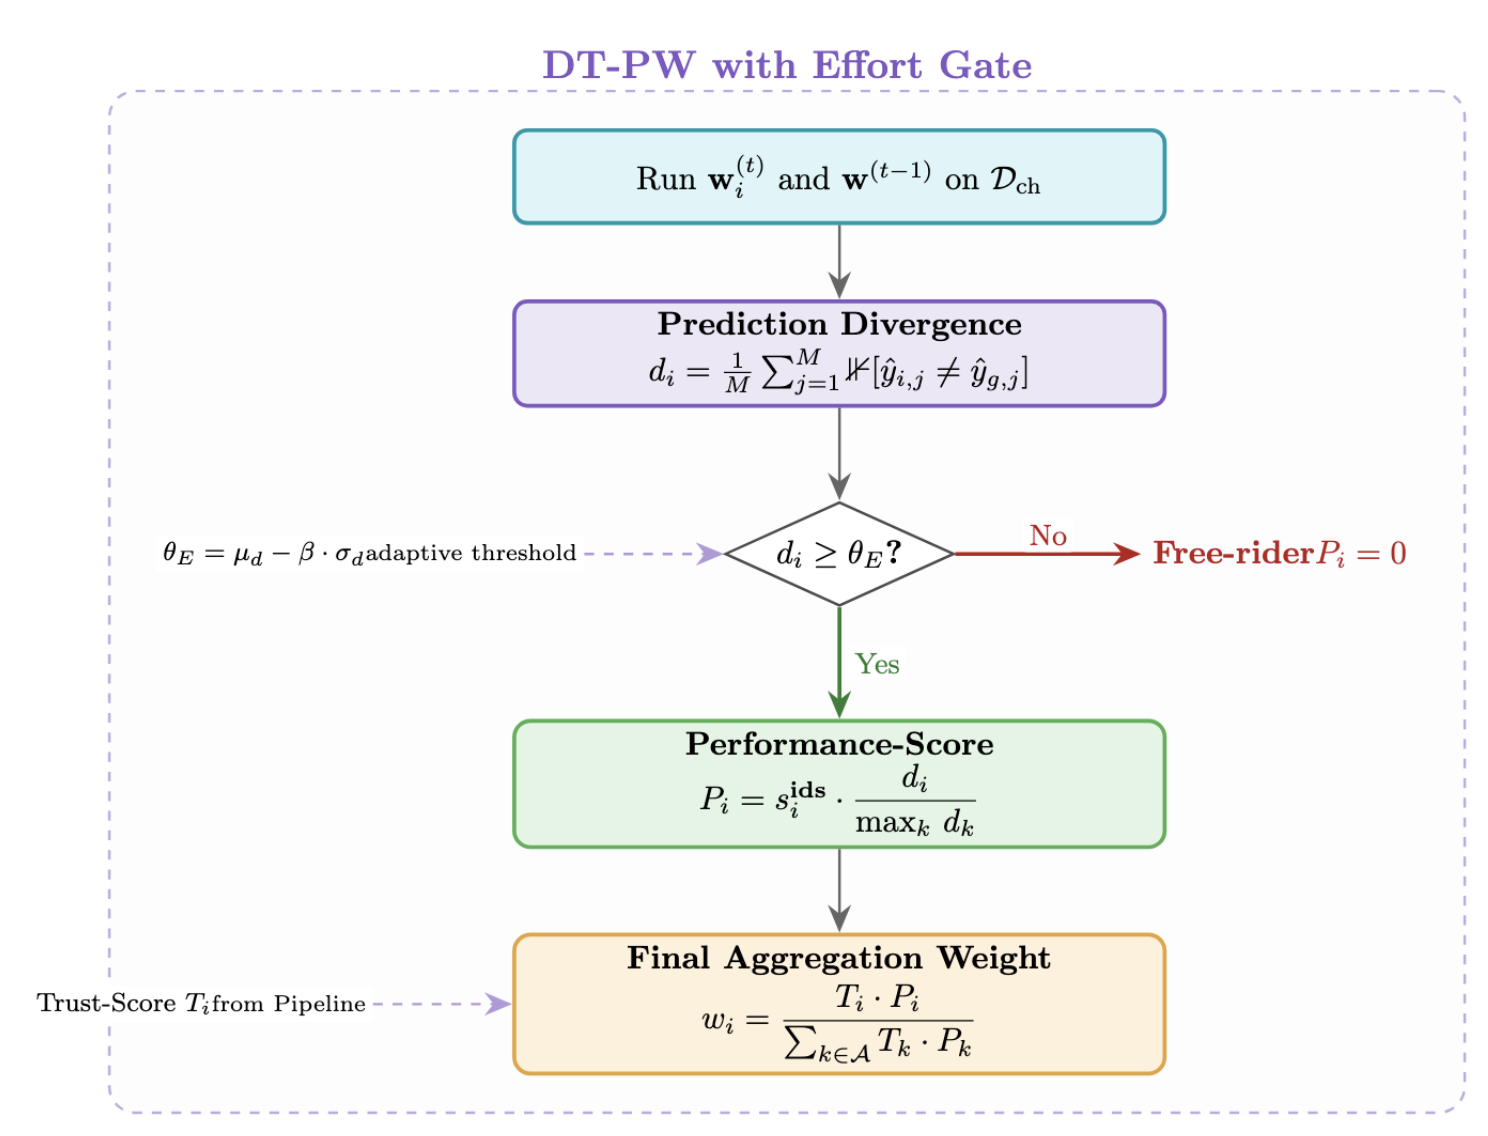
\includegraphics[width=0.85\linewidth]{Figures/fig_4_4_co_che_dtpw_effort_gate.png}
    \caption{Cơ chế DT-PW với Effort Gate}
\end{figure}

\subsection{Prediction Divergence}
Ý tưởng cốt lõi: client thực sự huấn luyện trên dữ liệu riêng sẽ học được tri thức mới mà mô hình toàn cục chưa có, dẫn đến dự đoán khác biệt trên $D_{\text{ch}}$. Free-rider chỉ sao chép $\mathbf{w}^{(t-1)}$ kèm nhiễu nhỏ, dự đoán gần như y hệt.

Cả $\mathbf{w}_{i}^{(t)}$ và $\mathbf{w}^{(t-1)}$ được nạp vào sandbox, chạy inference trên $D_{\text{ch}}$. Prediction divergence $d_{i}$ đo tỉ lệ mẫu có dự đoán khác nhau:

\begin{equation}
d_{i} = \frac{1}{M} \cdot \sum_{j = 1}^{M}\mathbb{1}\lbrack{\overset{\hat{}}{y}}_{i,j} \neq {\overset{\hat{}}{y}}_{g,j}\rbrack
\tag{4.8}
\end{equation}

Trong đó M = $|D_{\text{ch}}|$ là số mẫu, $\hat y_{i,j}$ = argmax $\mathbf{w}_{i}^{(t)}(x_{j})$ là dự đoán của mô hình cục bộ, $\hat y_{g,j}$ = argmax $\mathbf{w}^{(t-1)}(x_{j})$ là dự đoán của mô hình toàn cục, và $\mathbb{1}${[}$\cdot${]} là hàm chỉ thị (indicator function). Giá trị $d_{i}$ $\in$ {[}0, 1{]}:

\begin{itemize}
\item
  $d_{i}$ $\approx$ 0: Mô hình cục bộ dự đoán gần như y hệt mô hình toàn cục $\rightarrow$ free-rider.
\item
  $d_{i}$ \textgreater{} 0: Mô hình cục bộ có tri thức khác biệt $\rightarrow$ đã thực sự huấn luyện.
\end{itemize}

\subsection{Effort Gate}
Effort Gate phân biệt free-rider với client đóng góp thực sự bằng ngưỡng thích ứng. Ngưỡng $\theta_{E}$ được tính động dựa trên phân phối $\{d_{i}\}_{i\in\mathcal{T}}$ của tập client đã qua Trust Gate:

\begin{equation}
\theta_{E} = \mu_{d} - \beta \cdot \sigma_{d}
\tag{4.9}
\end{equation}

Trong đó $\mu_{d}$ = mean($\{d_{i}\}_{i\in\mathcal{T}}$) là trung bình, $\sigma_{d}$ = std($\{d_{i}\}_{i\in\mathcal{T}}$) là độ lệch chuẩn, và $\beta$ \textgreater 0 kiểm soát độ nhạy. $\beta$ lớn $\rightarrow$ ngưỡng thấp $\rightarrow$ ít client bị coi là free-rider; $\beta$ nhỏ $\rightarrow$ ngưỡng cao $\rightarrow$ nghiêm ngặt hơn.

Cơ chế ngưỡng thích ứng này quan trọng vì mức divergence "bình thường" thay đổi theo từng round (phụ thuộc vào mức hội tụ hiện tại, phân bổ dữ liệu, và loại tấn công). Thay vì dùng ngưỡng cố định (dễ quá nhạy hoặc quá lỏng), Effort Gate tự điều chỉnh dựa trên phân phối thực tế của round hiện tại.

Quyết định:

\begin{itemize}
\item
  Nếu $d_{i}$ \textless{} $\theta_{E}$: Client bị xem là free-rider $\rightarrow$ $P_{i}$ = 0.
\item
  Nếu $d_{i}$ $\geq$ $\theta_{E}$: Client được xem là đóng góp thực chất $\rightarrow$ được chấm Performance-Score.
\end{itemize}

\subsection{Performance-Score}
Đối với client vượt qua Effort Gate ($d_{i}$ $\geq$ $\theta_{E}$), Performance-Score kết hợp hai yếu tố: năng lực phát hiện xâm nhập (qua $s_{i}(ids)$ đã tính ở Lớp 1) và mức đóng góp tri thức mới (qua $d_{i}$ chuẩn hóa):

\begin{equation}
P_{i} = s_{i}(\text{ids}) \cdot \frac{d_{i}}{\max_{k}d_{k}}
\tag{4.10}
\end{equation}

Trong đó $max_{k}$ $d_{k}$ chuẩn hóa divergence về {[}0, 1{]}. Công thức đảm bảo: client có $s_{i}(ids)$ cao VÀ $d_{i}$ cao mới đạt $P_{i}$ cao. Client chỉ diverge nhiều nhưng phân loại kém (có thể do nhiễu) sẽ bị $s_{i}(ids)$ thấp kéo $P_{i}$ xuống.

\subsection{Trọng số tổng hợp cuối cùng}
Trọng số tổng hợp cho mỗi client kết hợp cả Trust-Score (độ tin cậy) và Performance-Score (mức đóng góp):

\begin{equation}
w_{i} = \frac{T_{i} \cdot P_{i}}{\sum_{k \in \mathcal{A}}^{}(T_{k} \cdot P_{k})}
\tag{4.11}
\end{equation}

Trong đó $\mathcal{A}$ là tập client được chấp nhận (qua cả Trust Gate và Effort Gate, có $P_{i}$ \textgreater 0). Mô hình toàn cục mới:

\begin{equation}
\mathbf{w}^{(t)} = \sum_{i \in \mathcal{A}}^{}w_{i} \cdot \mathbf{w}_{i}^{(t)}
\tag{4.12}
\end{equation}

Tính chất của công thức tổng hợp:

\begin{itemize}
\item
  Client bị Trust Gate loại ($T_{i}$ \textless{} $\theta_{T}$): Không thuộc $\mathcal{A},$ trọng số = 0.
\item
  Client bị Effort Gate loại ($d_{i}$ \textless{} $\theta_{E}$): $P_{i}$ = 0 $\rightarrow$ $w_{i}$ = 0.
\item
  Client đáng tin nhưng không đóng góp (free-rider): $T_{i}$ cao nhưng $P_{i}$ = 0 $\rightarrow$ $w_{i}$ = 0.
\item
  Client đóng góp nhưng không đáng tin (poisoner qua được Effort Gate): $P_{i}$ \textgreater{} 0 nhưng $T_{i}$ thấp $\rightarrow$ $w_{i}$ nhỏ.
\item
  Client vừa đáng tin vừa đóng góp: $T_{i}$ cao VÀ $P_{i}$ cao $\rightarrow$ $w_{i}$ lớn.
\end{itemize}

\section{Phân tích lý thuyết}

\subsection{Tại sao kiểm chứng hành vi vượt trội phân tích tham số thụ động}
Lợi thế của active behavioral verification có thể được phân tích qua bốn trường hợp điển hình:

Trường hợp 1 (Tấn công LIE {[}1{]}): LIE tạo tham số độc hại bằng cách cộng một lượng nhỏ vào giá trị trung bình của các bản cập nhật lành tính, giữ tham số trong vùng phân phối bình thường nên Krum, Median, GeoMed không phát hiện. Tuy nhiên, khi chạy trên challenge data, mô hình phân loại sai trên các lớp tấn công $\rightarrow$ điểm IDS Performance thấp $\rightarrow$ Trust Gate loại bỏ.

Trường hợp 2 (Tấn công Min-Max/Min-Sum {[}15{]}): Attacker tối ưu hóa bản cập nhật độc hại sao cho khoảng cách đến các update lành tính nằm trong giới hạn cho phép nên các bộ lọc khoảng cách thất bại. Nhưng hành vi phân loại bộc lộ trên challenge data $\rightarrow$ điểm IDS Performance thấp $\rightarrow$ bị loại.

Trường hợp 3 (Client Non-IID lành tính): Tham số của client lệch xa mô hình toàn cục do dữ liệu thiên lệch nên các phương pháp thụ động nhầm là tấn công (FPR cao). Nhưng mô hình vẫn phân loại chính xác trên challenge data (cân bằng nhãn) $\rightarrow$ điểm IDS Performance cao $\rightarrow$ vượt Trust Gate. Trong balanced mode, điểm IDS Performance cao (trọng số 0,7) bù cho điểm Parameter Similarity thấp (trọng số 0,3), đạt FPR = 0\%.

Trường hợp 4 (Free-rider): Tham số của free-rider gần như trùng với mô hình toàn cục (chỉ thêm nhiễu nhỏ) nên Trust-Score (LUP) thưởng 0,2448 (thực nghiệm). Nhưng prediction divergence gần bằng 0 $\rightarrow$ Effort Gate phát hiện $\rightarrow$ Performance-Score bằng 0 $\rightarrow$ trọng số = 0.

\subsection{Đảm bảo an toàn với sandbox isolation}
Digital Twin Sandbox cung cấp ba lớp đảm bảo an toàn:

\textbf{(1) Cách ly thực thi:} Mô hình được nạp vào sandbox dưới dạng bản sao tham số trên vùng nhớ riêng. Mọi thao tác (inference, gradient computation nếu có) chỉ ảnh hưởng đến vùng nhớ sandbox, không tác động đến FL Server hay mô hình toàn cục.

\textbf{(2) Reset sau kiểm chứng:} Sau mỗi lần kiểm tra, sandbox giải phóng toàn bộ tensor và context liên quan đến mô hình vừa kiểm tra, reset về trạng thái sạch trước khi nạp mô hình tiếp theo. Điều này ngăn chặn tấn công khai thác trạng thái tồn đọng.

\textbf{(3) Sequential loading:} Sandbox chỉ nạp một mô hình tại một thời điểm, giải phóng trước khi nạp mô hình kế tiếp. Cơ chế này vừa đảm bảo an toàn vừa tối ưu bộ nhớ, giúp peak memory thấp hơn cả FedAvg (phải giữ tất cả N bản cập nhật đồng thời).

\subsection{Độ phức tạp tính toán}
Chi phí tính toán bổ sung của DT-Guard mỗi round gồm hai thành phần:

\textbf{(1) Trust verification:} O(M $\times$ N), với M = $|D_{\text{ch}}|$ là số mẫu challenge data và N là số client. Mỗi client cần chạy inference M mẫu qua mạng IDS.

\textbf{(2) DT-PW scoring:} O(M $\times$ N), cần chạy inference cả mô hình cục bộ lẫn mô hình toàn cục trên M mẫu, rồi so sánh M cặp dự đoán.

Tổng overhead: O(M $\times$ N), được tối ưu nhờ pre-generated challenge pool (không sinh dữ liệu mới mỗi round) và sequential model loading. Thực nghiệm cho thấy overhead chiếm dưới 1\% tổng thời gian round.

\section{Tổng kết chương}
Chương này đã trình bày kiến trúc DT-Guard gồm năm thành phần chính: kiến trúc tổng thể 3 thực thể, bộ sinh TabDDPM, pipeline kiểm định 4 lớp với Trust-Score (Công thức 4.1--4.7), cơ chế DT-PW với Effort Gate (Công thức 4.8--4.12), và phân tích lý thuyết. Chương tiếp theo trình bày thực nghiệm và đánh giá trên hai bộ dữ liệu CIC-IoT-2023 và ToN-IoT.

% Chapter 5
\chapter{THỰC NGHIỆM VÀ ĐÁNH GIÁ}
\label{Chapter5}

Chương này báo cáo thực nghiệm trên CIC-IoT-2023 và ToN-IoT, gồm: thiết lập thực nghiệm, đánh giá phòng thủ, đánh giá bộ sinh, phát hiện free-rider, phân tích overhead, và bàn luận.

\section{Thiết lập thực nghiệm}

\subsection{Môi trường thực nghiệm}
\textbf{Phần cứng:} Toàn bộ thực nghiệm được thực hiện trên máy tính xách tay trang bị processor Apple M2 (8-core CPU, kiến trúc ARM64), bộ nhớ RAM 16 GB, không sử dụng GPU rời. Việc huấn luyện và suy luận mô hình đều chạy trên CPU thông qua PyTorch, phù hợp với mục tiêu đánh giá hiệu năng phòng thủ trong môi trường tài nguyên hạn chế, đặc trưng của các thiết bị edge IoT.

\textbf{Phần mềm:} Ngôn ngữ lập trình Python 3.11.6. Các thư viện chính: PyTorch 2.11.0 cho huấn luyện và suy luận mô hình học sâu; NumPy 1.24+ cho tính toán số; Pandas 2.0+ cho xử lý dữ liệu; scikit-learn 1.3+ cho các metric đánh giá; Matplotlib 3.7+ và Seaborn 0.12+ cho trực quan hóa. Mô hình sinh dữ liệu thách thức TabDDPM được xây dựng dựa trên thư viện diffusion models với kiến trúc MLP tùy chỉnh.

\textbf{Môi trường mô phỏng FL:} Hệ thống FL được xây dựng tùy chỉnh bằng Python, mô phỏng đầy đủ quy trình Federated Learning gồm: phân chia dữ liệu Non-IID theo phân phối Dirichlet, huấn luyện cục bộ trên từng client, tổng hợp tại server, và triển khai cả 9 phương pháp phòng thủ baseline. Môi trường mô phỏng cho phép kiểm soát hoàn toàn các biến số (tỉ lệ client độc hại, loại tấn công, seed ngẫu nhiên) nhằm đảm bảo so sánh công bằng giữa các phương pháp. Toàn bộ thực nghiệm sử dụng random seed cố định SEED = 42 để đảm bảo tính tái lập: np.random.seed(42) và torch.manual\_seed(42) được thiết lập trước mỗi kịch bản thực nghiệm.

\textbf{Ghi chú về mô phỏng:} Mô phỏng FL chạy tuần tự trên một máy đơn, mô phỏng hành vi của 20 client và 1 server trong cùng một tiến trình. Mặc dù thực tế FL chạy phân tán trên nhiều thiết bị, mô phỏng tuần tự là phương pháp chuẩn trong các nghiên cứu FL phòng thủ {[}1, 2, 5, 15, 16, 18, 19{]}, vì mục tiêu chính là đánh giá thuật toán phòng thủ (aggregation, filtering, scoring) chứ không phải hiệu năng giao tiếp mạng. Kết quả overhead thời gian (Mục 5.5) phản ánh chi phí tính toán của từng phương pháp, không bao gồm độ trễ mạng. Đây là thách thức của triển khai thực tế, nằm ngoài phạm vi đề tài.

\subsection{Cấu hình Federated Learning}
Cấu hình FL chung cho cả hai bộ dữ liệu: số client N = 20, số vòng lặp R = 20, batch size = 512, optimizer Adam (learning rate = $10^{-3}$), loss function Weighted Cross-Entropy, phân bổ dữ liệu Non-IID theo Dirichlet ($\alpha$ = 0,5). Mô hình IDS cho cả hai dataset là IoTAttackNet --- mạng MLP với kiến trúc input $\rightarrow$ 256 $\rightarrow$ 128 $\rightarrow$ 64 $\rightarrow$ num\_classes, sử dụng ReLU activation, BatchNorm, và Dropout (p = 0,3).

Các tham số được điều chỉnh theo từng bộ dữ liệu:

\begin{longtable}[]{@{}
  >{\raggedright\arraybackslash}p{(\linewidth - 4\tabcolsep) * \real{0.3642}}
  >{\raggedright\arraybackslash}p{(\linewidth - 4\tabcolsep) * \real{0.2243}}
  >{\raggedright\arraybackslash}p{(\linewidth - 4\tabcolsep) * \real{0.1567}}@{}}
\caption{Cấu hình thực nghiệm theo từng bộ dữ liệu} \\
\toprule\noalign{}
\begin{minipage}[b]{\linewidth}\centering
\textbf{Tham số}
\end{minipage} & \begin{minipage}[b]{\linewidth}\centering
\textbf{CIC-IoT-2023}
\end{minipage} & \begin{minipage}[b]{\linewidth}\centering
\textbf{ToN-IoT}
\end{minipage} \\
\midrule\noalign{}
\endfirsthead
%
\multicolumn{3}{c}{{\textit{(tiếp) Bảng 5.1}}} \\
\toprule\noalign{}
\begin{minipage}[b]{\linewidth}\centering
\textbf{Tham số}
\end{minipage} & \begin{minipage}[b]{\linewidth}\centering
\textbf{CIC-IoT-2023}
\end{minipage} & \begin{minipage}[b]{\linewidth}\centering
\textbf{ToN-IoT}
\end{minipage} \\
\midrule\noalign{}
\endhead
\bottomrule\noalign{}
\endlastfoot
Số đặc trưng / lớp & 39 / 34 & 10 / 10 \\
Local epochs (E) & 3 & 2 \\
Ngưỡng Trust-Score ($\theta_{T}$) & 0,6 & 0,5 \\
Số mẫu challenge & 200 & 500 \\
\end{longtable}

Tỉ lệ client độc hại được đánh giá ở bốn mức: 10\% (2 client), 20\% (4 client), 40\% (8 client), và 50\% (10 client), từ mức nhẹ đến mức khắc nghiệt nhất.

\subsection{Các phương pháp đối sánh}
DT-Guard được so sánh với chín phương pháp phòng thủ đại diện, phân thành ba nhóm:

\begin{itemize}
\item
  \textbf{Không phòng thủ:} FedAvg {[}9{]}
\item
  \textbf{Thống kê cổ điển:} Krum {[}2{]}, Median {[}18{]}, Trimmed Mean {[}18{]}, GeoMed {[}12{]}
\item
  \textbf{Phân tích nâng cao:} SignGuard {[}16{]}, ClipCluster {[}19{]}, LUP {[}5{]}, PoC {[}22{]}
\end{itemize}

\subsection{Các chỉ số đánh giá}
Ba chỉ số chính được sử dụng:

\begin{itemize}
\item
  \textbf{Accuracy:} Hiệu năng phát hiện xâm nhập của mô hình toàn cục trên tập kiểm tra.
\item
  \textbf{Detection Rate (DR):} Tỉ lệ client độc hại bị DT-Guard phát hiện và loại bỏ chính xác.
\item
  \textbf{False Positive Rate (FPR):} Tỉ lệ client lành tính bị loại nhầm.
\end{itemize}

\subsection{Kịch bản thực nghiệm}
Thực nghiệm gồm ba kịch bản:

Kịch bản A (Đánh giá hiệu năng phòng thủ): 5 loại tấn công (Backdoor, LIE, Min-Max, Min-Sum, MPAF) $\times$ 4 mức tỉ lệ malicious (10\%, 20\%, 40\%, 50\%) = 20 kịch bản trên mỗi dataset (CIC-IoT-2023 và ToN-IoT), tổng cộng 40 kịch bản.

Kịch bản B (Đánh giá bộ sinh dữ liệu thách thức): A/B Testing 5 mô hình sinh (TabDDPM, TabSyn, ForestDiffusion, CTGAN, WGAN-GP).

Kịch bản C (Đánh giá tính công bằng và phát hiện free-rider): 4 free-rider trong 20 client, so sánh 4 chiến lược tổng hợp.

\subsection{Phân tích khám phá dữ liệu (EDA)}
\label{sec:eda}
Trước khi thực hiện các kịch bản chính, phần này phân tích chi tiết đặc điểm của hai bộ dữ liệu nhằm làm rõ năm yếu tố ảnh hưởng trực tiếp đến hiệu năng phòng thủ: phân phối lớp tổng thể, thống kê mô tả đặc trưng, phân phối giá trị đặc trưng, label skew và feature skew sau khi phân chia Dirichlet.

\subsubsection{Phân phối lớp tổng thể trước khi chia train--test}
Bảng \ref{tab:cic_class_dist} thống kê phân phối mẫu theo danh mục tấn công trên \textit{toàn bộ} dataset CIC-IoT-2023 gốc (46,7 triệu mẫu, gộp 63 file CSV, theo công bố chính thức {[}11{]}); thực nghiệm sử dụng slice Merged01.csv (712.311 mẫu) làm tập đại diện vì phân phối tương đối được bảo toàn (DDoS $\approx$72,3\% so với 72,82\% trên toàn bộ). Dữ liệu mất cân bằng cực kỳ nghiêm trọng: DDoS chiếm 72,82\%, trong khi BruteForce chỉ chiếm 0,03\%---tỷ lệ chênh lệch $\sim$2.600$\times$.

\begin{table}[H]
\centering
\caption{Phân phối mẫu theo danh mục tấn công trong CIC-IoT-2023 (toàn bộ dataset gốc) {[}11{]}}
\label{tab:cic_class_dist}
\small
\begin{tabular}{|l|r|r|}
\hline
\textbf{Danh mục} & \textbf{Số dòng} & \textbf{Tỷ lệ (\%)} \\
\hline
DDoS & 33.984.560 & 72,82 \\
\hline
DoS & 8.090.738 & 17,34 \\
\hline
Mirai & 2.634.124 & 5,64 \\
\hline
Benign & 1.098.195 & 2,35 \\
\hline
Spoofing & 486.504 & 1,04 \\
\hline
Reconnaissance & 354.565 & 0,76 \\
\hline
Web-based & 24.829 & 0,05 \\
\hline
BruteForce & 13.064 & 0,03 \\
\hline
\textbf{Tổng} & \textbf{46.686.579} & \textbf{100,00} \\
\hline
\end{tabular}
\end{table}

Bảng \ref{tab:ton_iot_class_dist} thống kê phân phối ToN-IoT (toàn bộ dataset đã tiền xử lý). Đặc thù nổi bật: Normal chiếm 65\%, 8 lớp tấn công có $\sim$20.000 mẫu mỗi lớp, MITM chỉ 1.042 mẫu---mất cân bằng kiểu \textit{one-vs-many}.

\begin{table}[H]
\centering
\caption{Phân phối mẫu theo loại tấn công trong ToN-IoT {[}10{]}}
\label{tab:ton_iot_class_dist}
\small
\begin{tabular}{|l|r|r|}
\hline
\textbf{Loại} & \textbf{Số mẫu} & \textbf{Tỷ lệ (\%)} \\
\hline
Normal & 300.000 & 65,07 \\
\hline
Scanning & 20.000 & 4,34 \\
\hline
DoS & 20.000 & 4,34 \\
\hline
DDoS & 20.000 & 4,34 \\
\hline
Ransomware & 20.000 & 4,34 \\
\hline
Backdoor & 20.000 & 4,34 \\
\hline
Injection & 20.000 & 4,34 \\
\hline
XSS & 20.000 & 4,34 \\
\hline
Password & 20.000 & 4,34 \\
\hline
MITM & 1.042 & 0,23 \\
\hline
\textbf{Tổng} & \textbf{461.042} & \textbf{100,00} \\
\hline
\end{tabular}
\end{table}

Hai dạng mất cân bằng này (\textit{long-tail} ở CIC-IoT-2023 và \textit{one-vs-many} ở ToN-IoT) là cơ sở để áp dụng Weighted Cross-Entropy Loss (Mục~\ref{subsec:wce_loss}) và là nguồn gốc tự nhiên của \textit{label skew} sau khi phân chia Dirichlet (chi tiết tại Mục~\ref{subsec:eda_dirichlet}).

\subsubsection{Thống kê mô tả đặc trưng}
Bảng \ref{tab:cic_iot_feature_stats} thống kê đầy đủ 39 đặc trưng của CIC-IoT-2023, chia thành 5 nhóm: thông tin header mạng (4), cờ TCP (7), số lượng cờ (4), chỉ báo giao thức (15) và thống kê gói tin (9). Phần lớn đặc trưng chỉ báo giao thức (Telnet, SSH, IRC, SMTP, IGMP, DHCP) có giá trị trung bình $\approx 0$, cho thấy chúng hiếm khi xuất hiện trong lưu lượng IoT. Các đặc trưng liên tục như Variance (std $= 411{,}9$K) và Rate (max $= 5{,}2$M) trải rất rộng, phản ánh sự đa dạng mạnh của lưu lượng. Đối với ToN-IoT, dữ liệu đã được chuẩn hoá StandardScaler trước khi công bố nên 10 đặc trưng đều nằm trong dải chuẩn (mean$\approx$0, var$\in[0{,}03; 0{,}13]$); thống kê chi tiết được trình bày gián tiếp qua phân phối ở Mục~\ref{subsec:eda_value_dist}.

\begin{footnotesize}
\begin{longtable}{|l|l|r|r|r|r|}
\caption{Thống kê mô tả 39 đặc trưng CIC-IoT-2023 ($n = 712{.}311$ mẫu)} \label{tab:cic_iot_feature_stats} \\
\hline
\textbf{Đặc trưng} & \textbf{Loại} & \textbf{Mean} & \textbf{Std} & \textbf{Min} & \textbf{Max} \\
\hline
\endfirsthead
\hline
\textbf{Đặc trưng} & \textbf{Loại} & \textbf{Mean} & \textbf{Std} & \textbf{Min} & \textbf{Max} \\
\hline
\endhead
\multicolumn{6}{|l|}{\textit{Thông tin header mạng}} \\
\hline
Header\_Length & Liên tục & 13,76 & 8,72 & 0 & 60 \\
\hline
Protocol Type & Phân loại & 9,09 & 9,08 & 0 & 47 \\
\hline
Time\_To\_Live & Liên tục & 66,53 & 14,38 & 0 & 255 \\
\hline
Rate & Liên tục & 28,4K & 30,2K & 0,001 & 5,2M \\
\hline
\multicolumn{6}{|l|}{\textit{Cờ TCP}} \\
\hline
fin\_flag\_number & Nhị phân & 0,088 & 0,280 & 0 & 1 \\
\hline
syn\_flag\_number & Nhị phân & 0,207 & 0,400 & 0 & 1 \\
\hline
rst\_flag\_number & Nhị phân & 0,093 & 0,284 & 0 & 1 \\
\hline
psh\_flag\_number & Nhị phân & 0,094 & 0,277 & 0 & 1 \\
\hline
ack\_flag\_number & Nhị phân & 0,130 & 0,317 & 0 & 1 \\
\hline
ece\_flag\_number & Nhị phân & $\approx$0 & 0,002 & 0 & 0,6 \\
\hline
cwr\_flag\_number & Nhị phân & $\approx$0 & 0,002 & 0 & 0,6 \\
\hline
\multicolumn{6}{|l|}{\textit{Số lượng cờ (0--100)}} \\
\hline
ack\_count & Đếm & 9,87 & 28,05 & 0 & 100 \\
\hline
syn\_count & Đếm & 20,42 & 39,92 & 0 & 100 \\
\hline
fin\_count & Đếm & 8,66 & 28,01 & 0 & 100 \\
\hline
rst\_count & Đếm & 9,22 & 28,30 & 0 & 100 \\
\hline
\multicolumn{6}{|l|}{\textit{Chỉ báo giao thức}} \\
\hline
HTTP & Nhị phân & 0,050 & 0,214 & 0 & 1 \\
\hline
HTTPS & Nhị phân & 0,059 & 0,220 & 0 & 1 \\
\hline
DNS & Nhị phân & 0,003 & 0,022 & 0 & 1 \\
\hline
Telnet & Nhị phân & $\approx$0 & 0,001 & 0 & 0,3 \\
\hline
SMTP & Nhị phân & $\approx$0 & 0,001 & 0 & 0,4 \\
\hline
SSH & Nhị phân & $\approx$0 & 0,008 & 0 & 1 \\
\hline
IRC & Nhị phân & $\approx$0 & 0,001 & 0 & 0,2 \\
\hline
TCP & Nhị phân & 0,576 & 0,485 & 0 & 1 \\
\hline
UDP & Nhị phân & 0,217 & 0,401 & 0 & 1 \\
\hline
DHCP & Nhị phân & $\approx$0 & 0,005 & 0 & 0,5 \\
\hline
ARP & Nhị phân & 0,003 & 0,019 & 0 & 1 \\
\hline
ICMP & Nhị phân & 0,163 & 0,366 & 0 & 1 \\
\hline
IGMP & Nhị phân & $\approx$0 & 0,001 & 0 & 0,2 \\
\hline
IPv & Nhị phân & 0,997 & 0,019 & 0 & 1 \\
\hline
LLC & Nhị phân & 0,997 & 0,019 & 0 & 1 \\
\hline
\multicolumn{6}{|l|}{\textit{Thống kê gói tin}} \\
\hline
Tot sum & Liên tục & 10,9K & 16,8K & 60 & 239,4K \\
\hline
Min & Liên tục & 79,88 & 106,88 & 42 & 3,0K \\
\hline
Max & Liên tục & 222,50 & 586,94 & 54 & 30,5K \\
\hline
AVG & Liên tục & 130,90 & 227,67 & 48,4 & 5,4K \\
\hline
Std & Liên tục & 41,12 & 181,58 & 0 & 9,5K \\
\hline
Tot size & Liên tục & 130,90 & 227,67 & 48,4 & 5,4K \\
\hline
IAT & Liên tục & 0,002 & 0,883 & 0 & 741 \\
\hline
Number & Đếm & 95,51 & 19,56 & 1 & 100 \\
\hline
Variance & Liên tục & 34,7K & 411,9K & 0 & 90,9M \\
\hline
\end{longtable}
\end{footnotesize}

\subsubsection{Phân phối giá trị đặc trưng}
\label{subsec:eda_value_dist}
Hình \ref{fig:cic_iot_feature_dist} minh họa phân phối giá trị của 8 đặc trưng liên tục đại diện trong CIC-IoT-2023. Đa số đặc trưng có phân phối lệch phải nặng: phần lớn mẫu tập trung ở giá trị thấp, trong khi một tỷ lệ nhỏ có giá trị rất cao---dấu hiệu của tấn công burst tạo outlier. Nhiều đặc trưng (Std, Variance, IAT) tập trung ở giá trị 0, phản ánh thực tế rằng nhiều flow ngắn có tất cả gói tin cùng kích thước. Một số đặc trưng như Rate và Variance có giá trị trải dài qua nhiều cấp độ lớn, cho thấy lưu lượng IoT rất đa dạng và đòi hỏi chuẩn hóa phù hợp.

\begin{figure}[H]
    \centering
    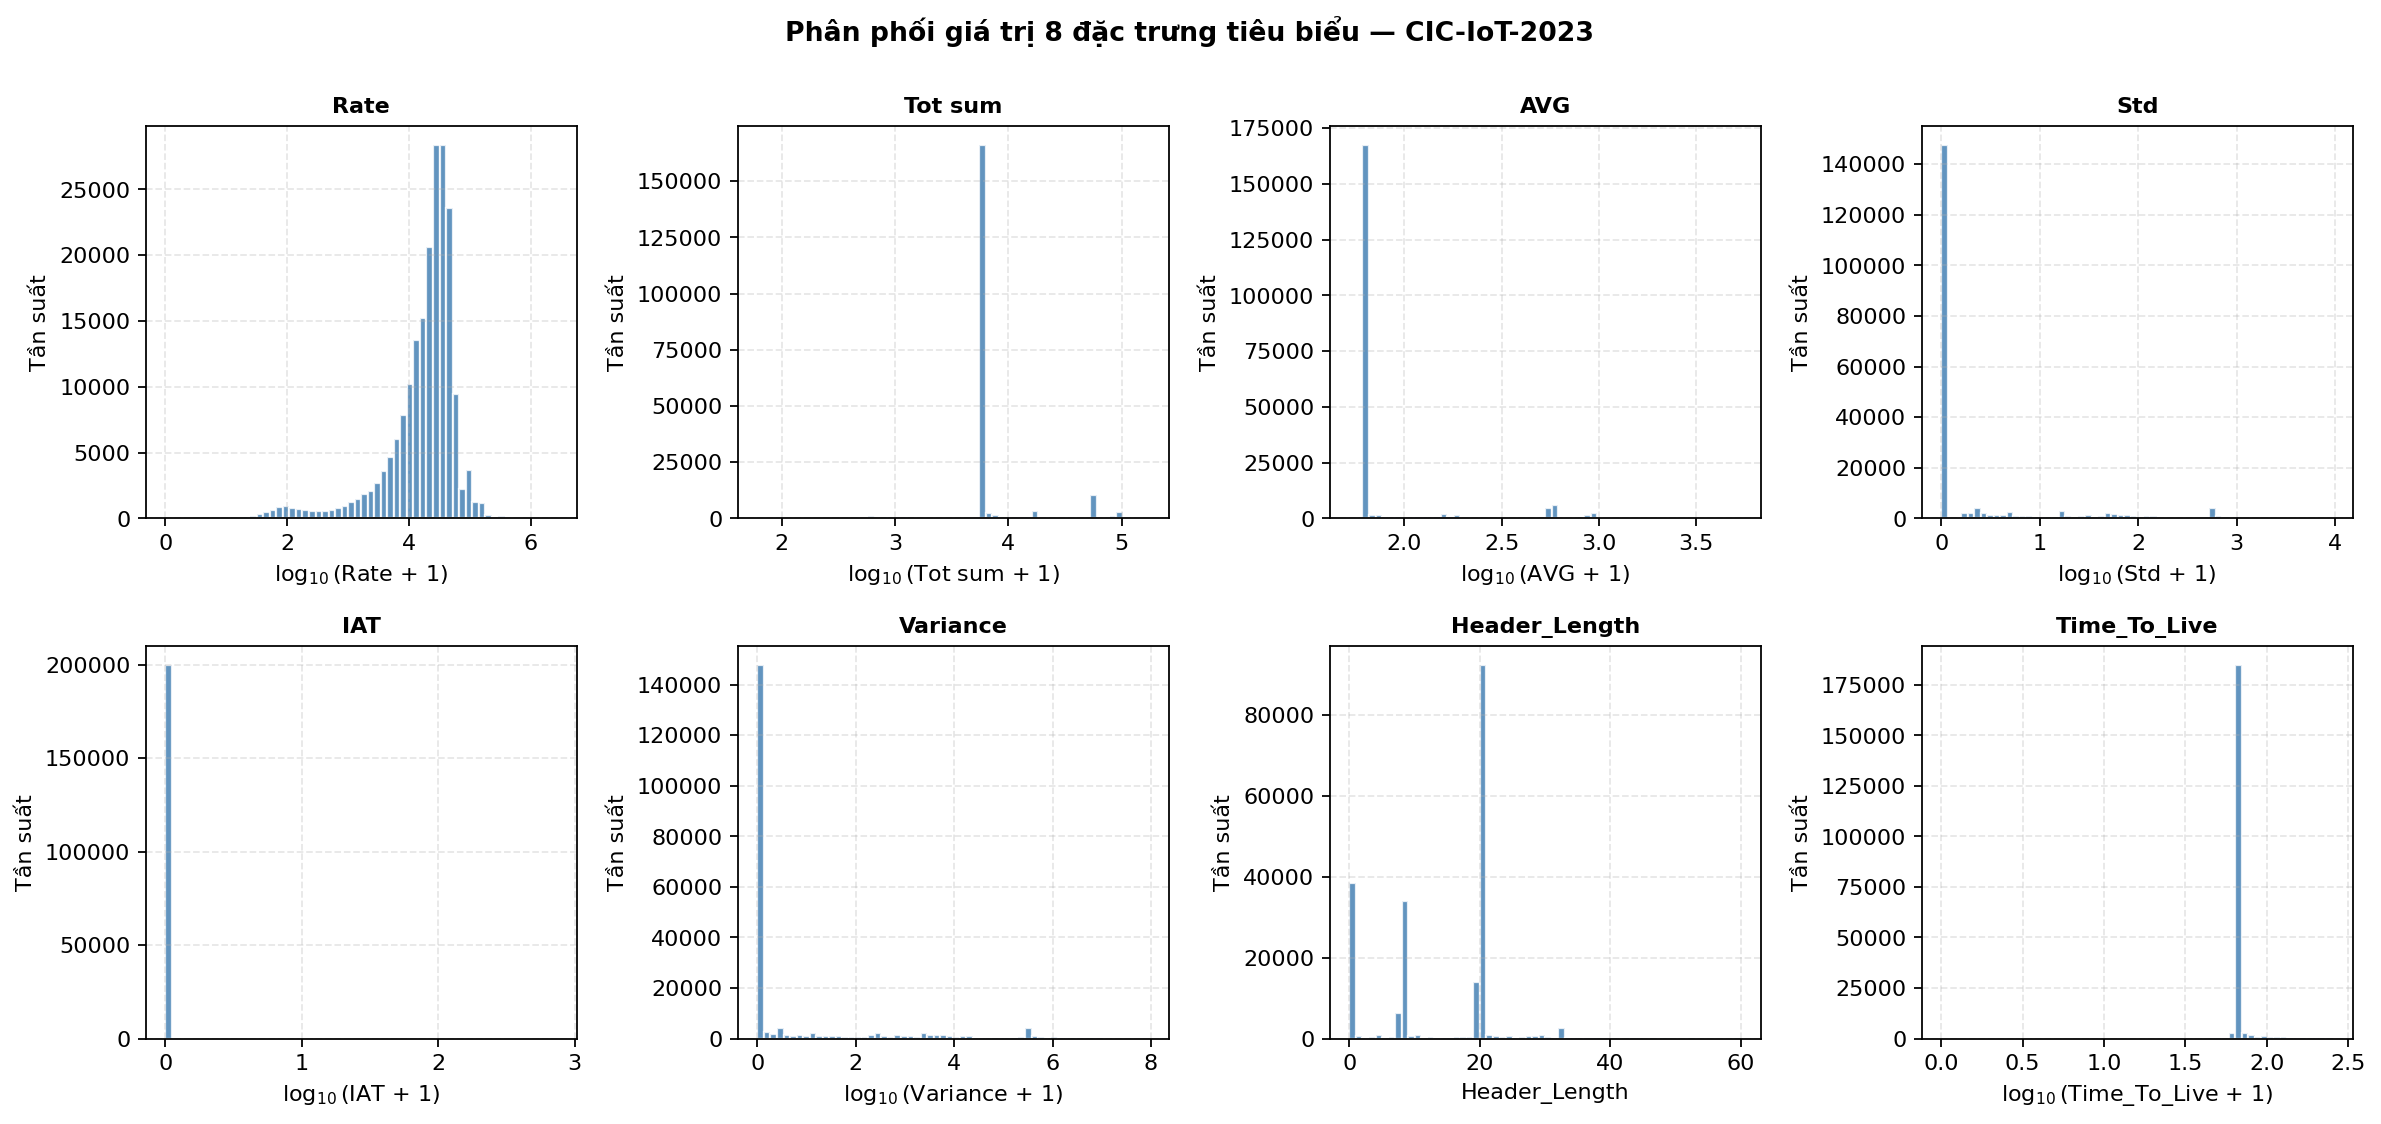
\includegraphics[width=0.90\linewidth]{Figures/fig_5_1_cic_iot_feature_dist.png}
    \caption{Phân phối giá trị 8 đặc trưng liên tục đại diện trong CIC-IoT-2023}
    \label{fig:cic_iot_feature_dist}
\end{figure}

Hình \ref{fig:ton_iot_feature_dist} minh họa phân phối 10 đặc trưng ToN-IoT sau chuẩn hóa StandardScaler. So với CIC-IoT-2023, các đặc trưng có phân phối đa đỉnh (multi-modal), mỗi đỉnh tương ứng với một nhóm loại tấn công. Đặc trưng có khoảng giá trị hẹp hơn và phân phối ổn định hơn, phản ánh việc đã chọn lọc 10 đặc trưng quan trọng nhất từ 44 đặc trưng ban đầu.

\begin{figure}[H]
    \centering
    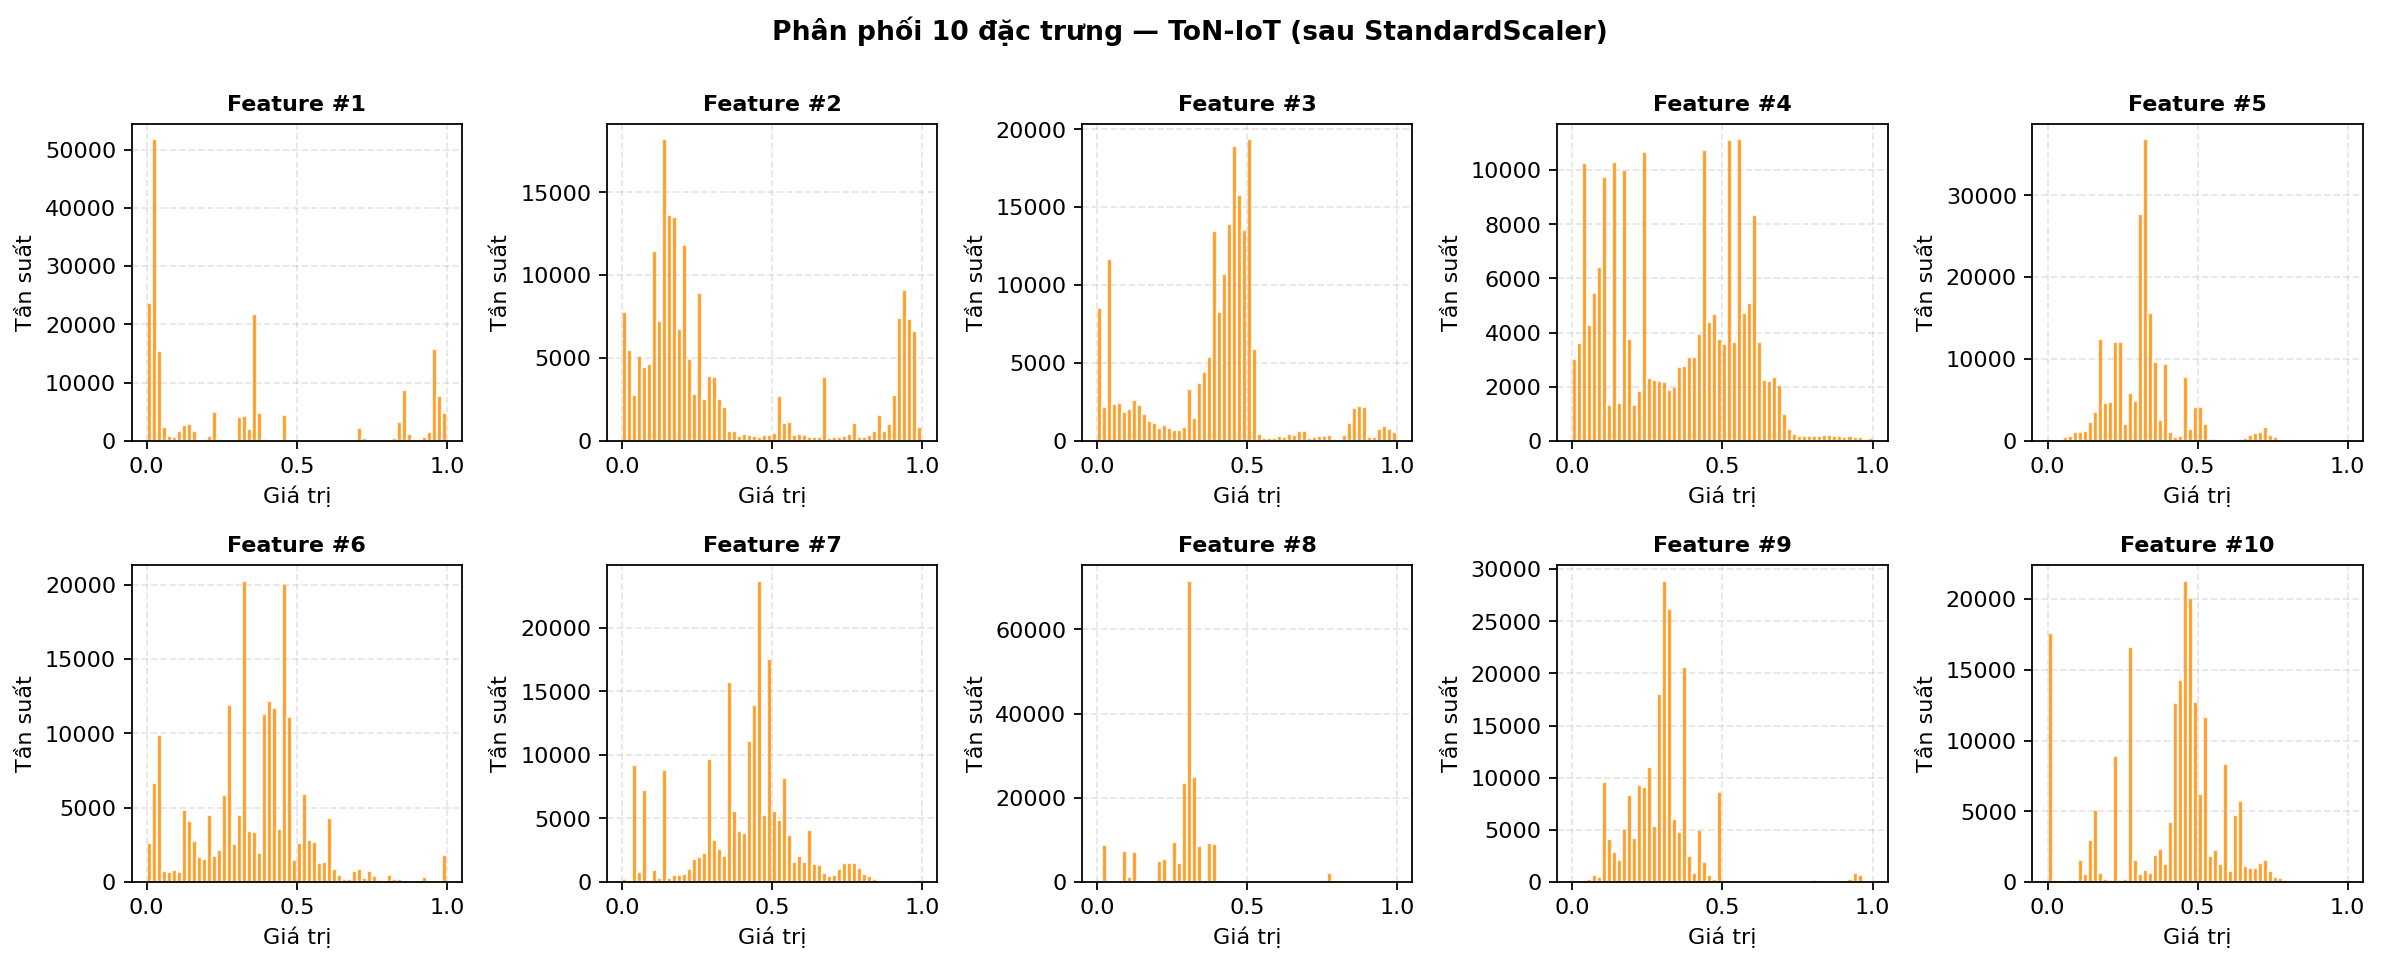
\includegraphics[width=0.90\linewidth]{Figures/fig_5_2_ton_iot_feature_dist.png}
    \caption{Phân phối giá trị 10 đặc trưng trong ToN-IoT (sau StandardScaler)}
    \label{fig:ton_iot_feature_dist}
\end{figure}

\subsubsection{Phân chia Dirichlet và mức độ Non-IID (label skew)}
\label{subsec:eda_dirichlet}
Hình \ref{fig:cic_iot_dirichlet_split} và Hình \ref{fig:ton_iot_dirichlet_split} trực quan hóa kết quả phân chia Dirichlet trên cả hai dataset với 10 client. Khi $\alpha=0{,}1$, mỗi client gần như chỉ chứa 1--2 lớp (label skew cực đoan); khi $\alpha=0{,}5$, phân phối đa dạng hơn nhưng vẫn chênh lệch đáng kể.

\textbf{CIC-IoT-2023 (Hình \ref{fig:cic_iot_dirichlet_split}):} Với $\alpha=0{,}1$, một số client bị chi phối bởi một loại tấn công DDoS/DoS duy nhất chiếm trên 60\% mẫu (ví dụ DDOS-UDP\_FLOOD 62\% ở C1, DOS-SYN\_FLOOD 78\% ở C4, DDOS-TCP\_FLOOD 64\% ở C8), trong khi các client khác chỉ nhận được dưới 3.000 mẫu (C10 chỉ 1.414 mẫu). Sự chênh lệch số mẫu giữa client lớn nhất (C5, $\sim$48 nghìn) và nhỏ nhất (C10) lên đến $\sim$34$\times$. Với $\alpha=0{,}5$, sự phân tán giảm rõ rệt: lớp tấn công đứng đầu ở mỗi client chỉ chiếm 15--43\% (không client nào còn vượt 50\%), và độ chênh số mẫu thu hẹp xuống $\sim$5$\times$. Các lớp thiểu số (BruteForce, XSS, Web-based) gần như không hiển thị trên biểu đồ do tỷ lệ quá nhỏ, cho thấy 34 lớp tấn công tạo ra Non-IID phức tạp hơn nhiều so với bộ dữ liệu chỉ có 10 lớp.

\textbf{ToN-IoT (Hình \ref{fig:ton_iot_dirichlet_split}):} Với $\alpha=0{,}1$, một số client gần như chỉ chứa một lớp (ví dụ C8 có 99,6\% là DoS, C4 có 93,7\% là Normal, C10 có 86\% là XSS, C2 có 82\% là Ransomware). Sự chênh lệch số mẫu giữa client lớn nhất (C4, $\sim$151 nghìn) và nhỏ nhất (C3, 476 mẫu) lên đến $\sim$318$\times$. Với $\alpha=0{,}5$, phân phối cân bằng hơn nhưng Normal vẫn chiếm đa số ở 6/10 client (39--78\%), độ chênh số mẫu giảm xuống $\sim$15$\times$. MITM---lớp hiếm nhất---hoàn toàn vắng mặt ở 5/10 client khi $\alpha=0{,}1$ và chỉ xuất hiện thưa thớt khi $\alpha=0{,}5$, tạo thách thức lớn cho phát hiện tấn công hiếm trong môi trường phân tán.

\begin{figure}[H]
    \centering
    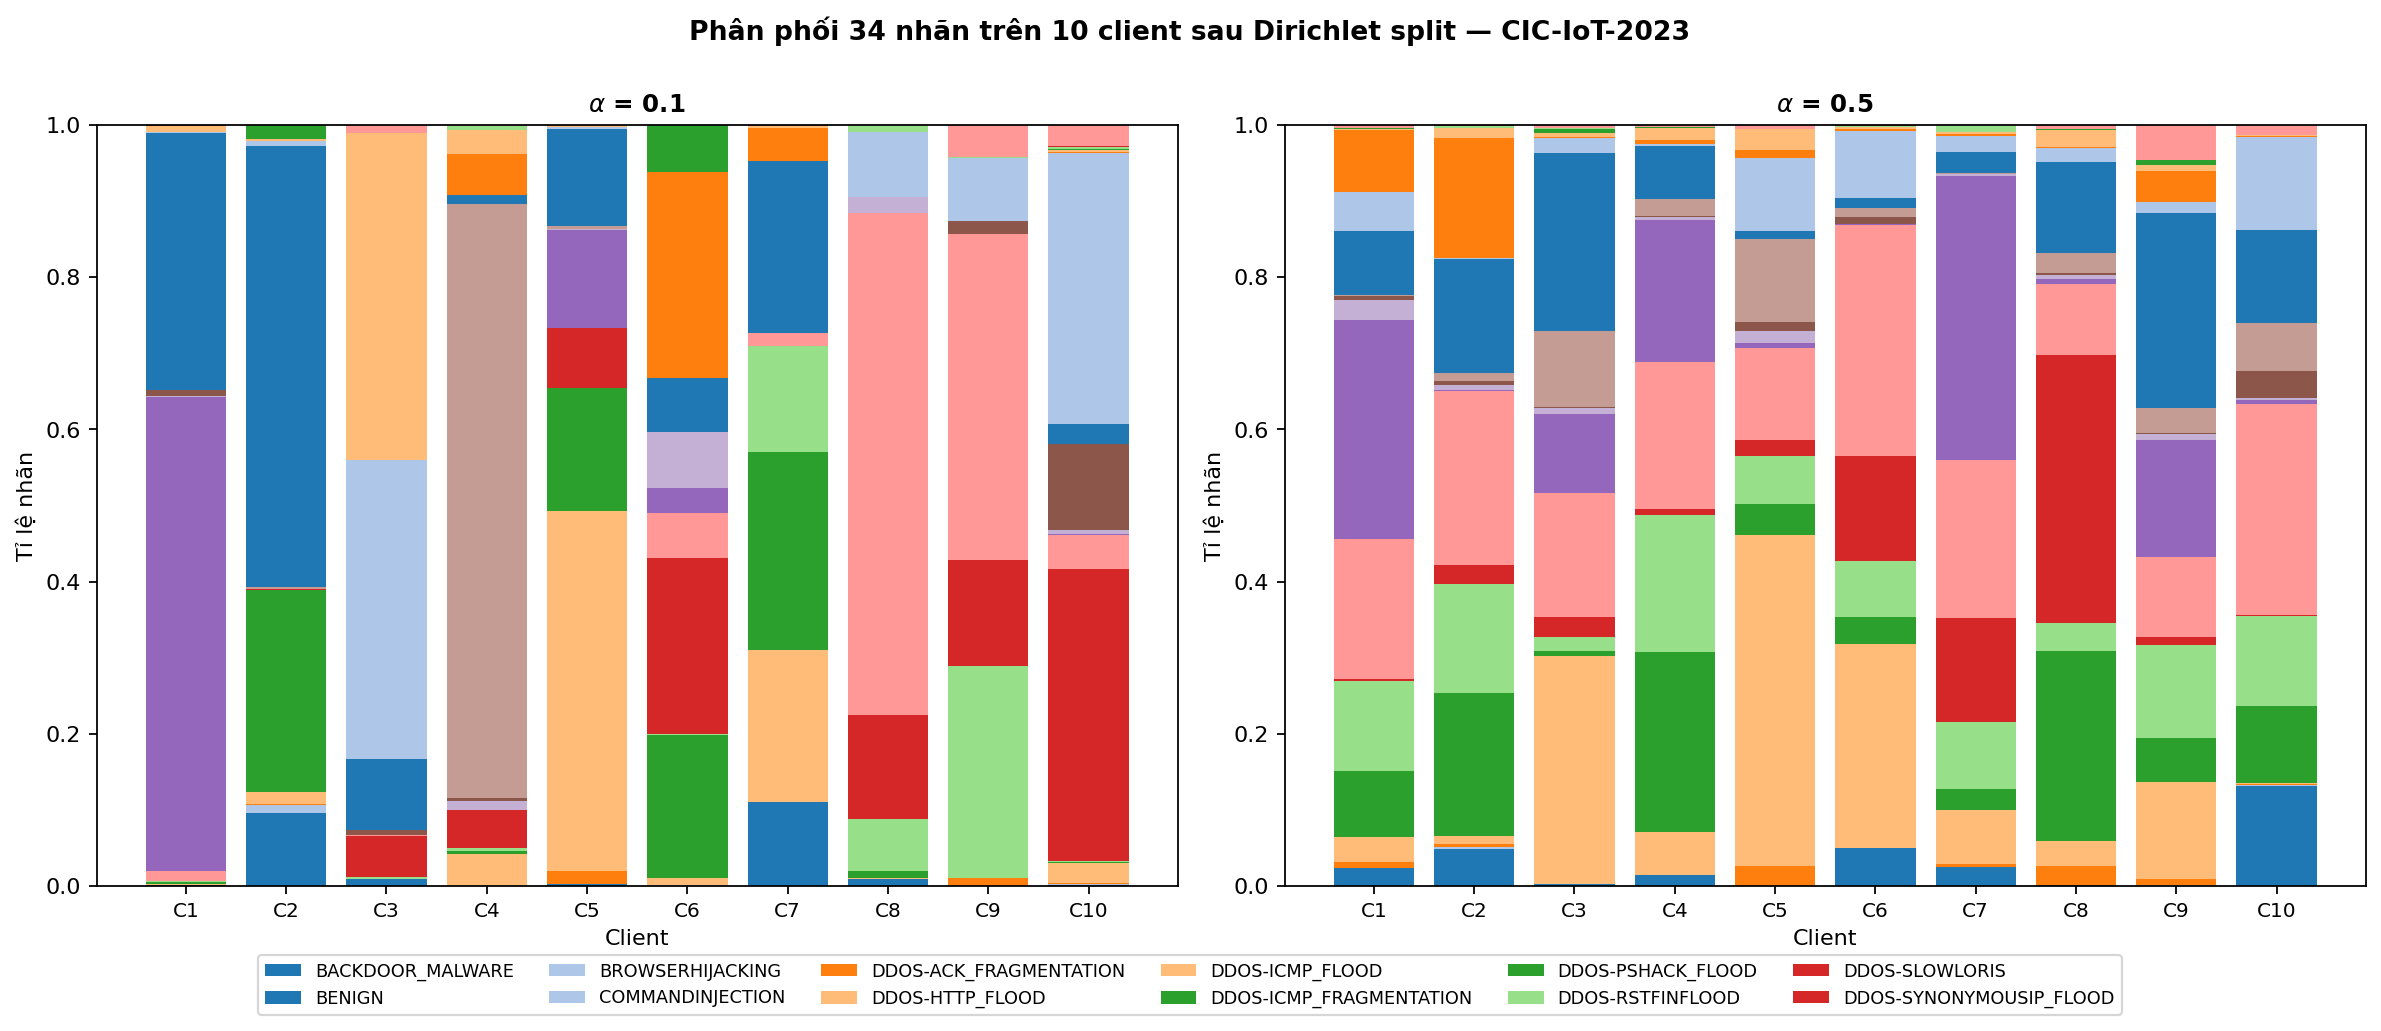
\includegraphics[width=0.95\linewidth]{Figures/fig_5_3_cic_iot_dirichlet_split.png}
    \caption{Phân phối 34 nhãn trên 10 client sau Dirichlet splitting -- CIC-IoT-2023 (trái: $\alpha=0{,}1$, phải: $\alpha=0{,}5$)}
    \label{fig:cic_iot_dirichlet_split}
\end{figure}

\begin{figure}[H]
    \centering
    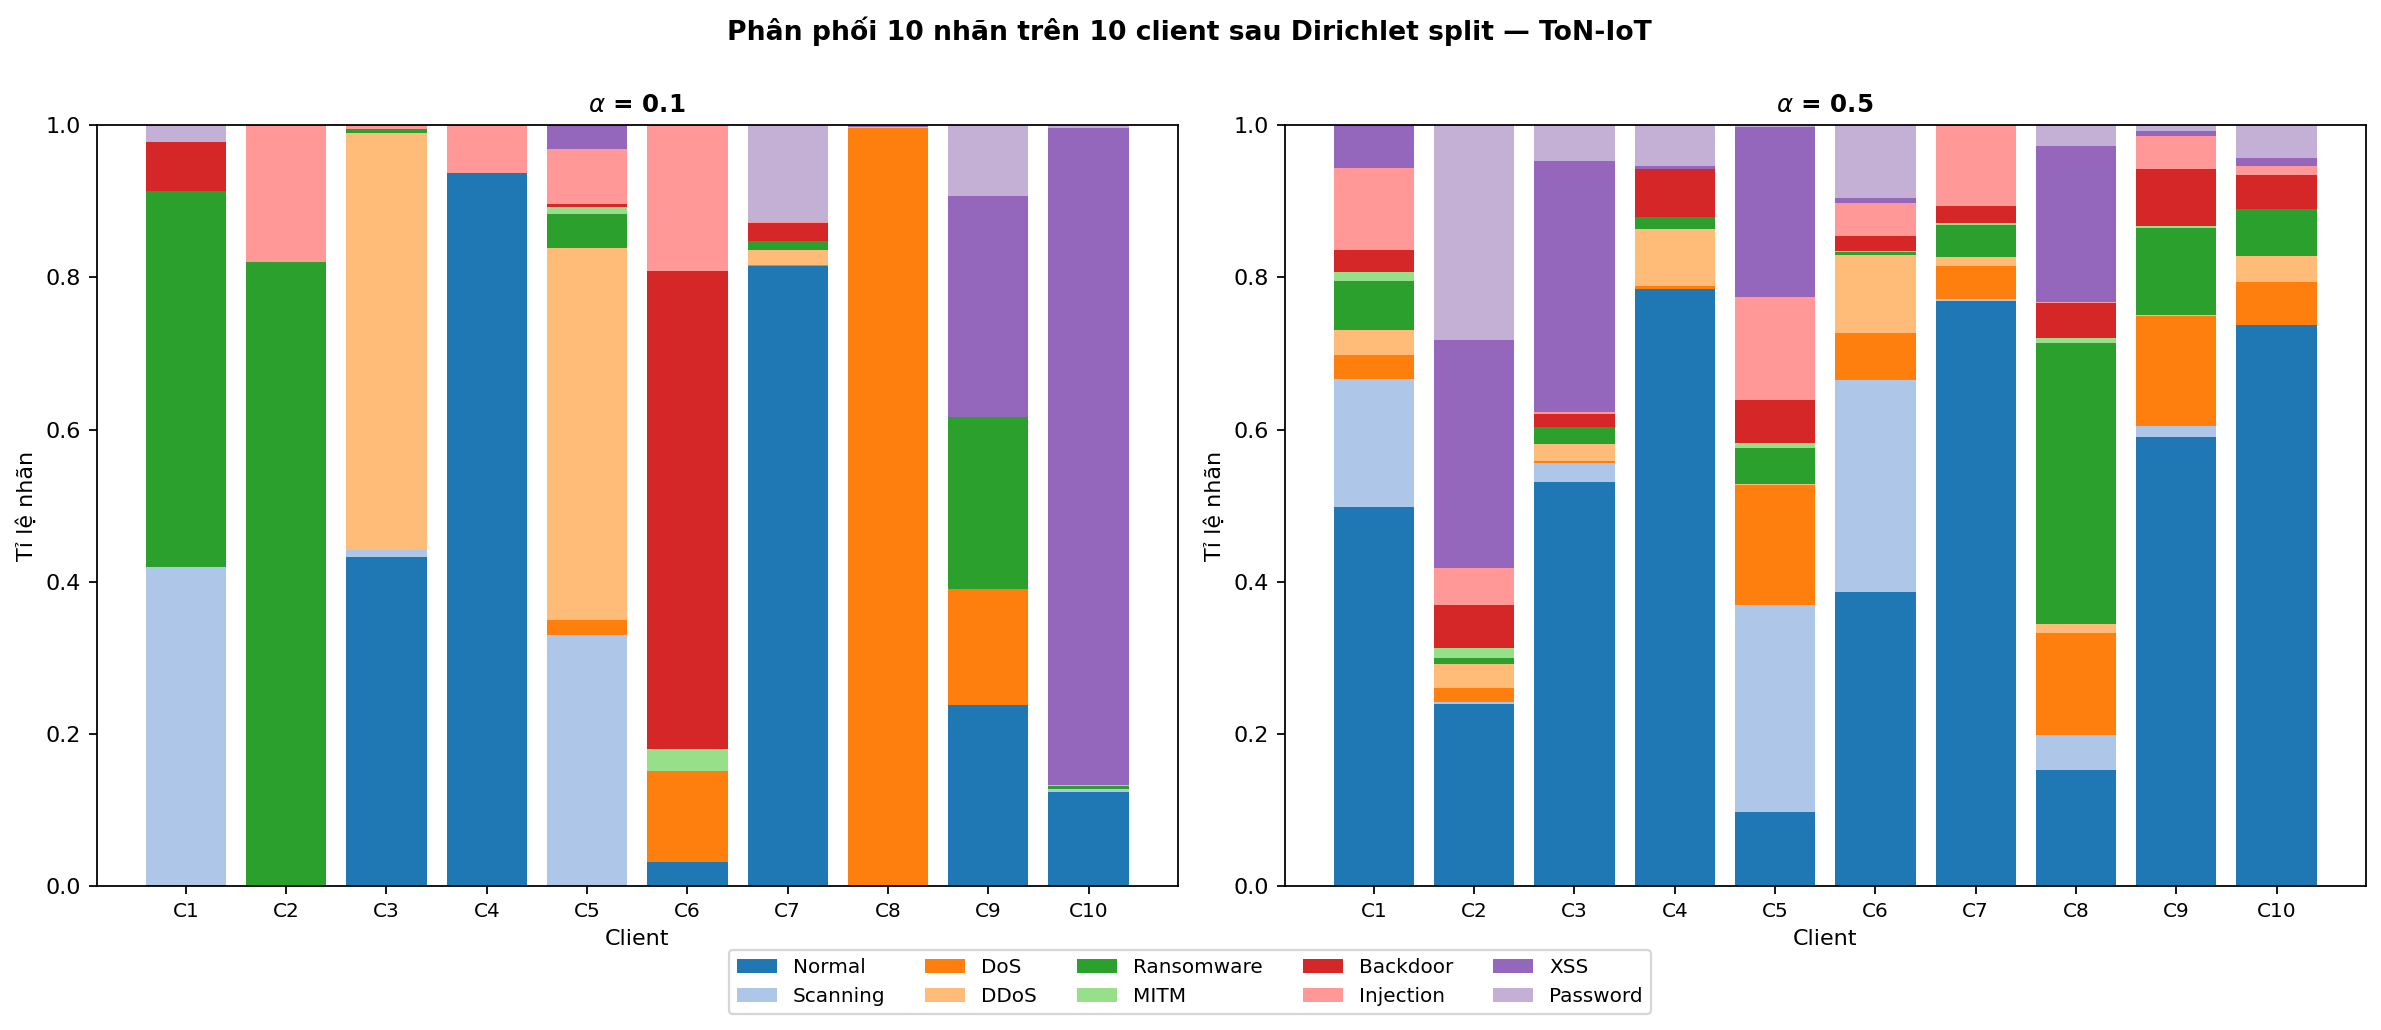
\includegraphics[width=0.95\linewidth]{Figures/fig_5_4_ton_iot_dirichlet_split.png}
    \caption{Phân phối 10 nhãn trên 10 client sau Dirichlet splitting -- ToN-IoT (trái: $\alpha=0{,}1$, phải: $\alpha=0{,}5$)}
    \label{fig:ton_iot_dirichlet_split}
\end{figure}

\subsubsection{Phân phối giá trị đặc trưng theo client (feature skew)}
\label{subsec:eda_feature_skew}
Bên cạnh \textit{label skew}, Dirichlet splitting còn gây ra \textit{feature skew} (Mục 3.1.3): cùng một đặc trưng nhưng phân phối giá trị giữa các client khác nhau rõ rệt do mỗi client tập trung vào tập lớp riêng. Hình \ref{fig:cic_iot_feat_skew} và Hình \ref{fig:ton_iot_feat_skew} minh hoạ hiện tượng này bằng boxplot của các đặc trưng tiêu biểu trên 10 client sau khi split.

\textbf{Lý do chọn đặc trưng minh hoạ.} Không gian đặc trưng quá lớn để vẽ toàn bộ (39 cột với CIC-IoT-2023, 10 cột với ToN-IoT), nên mỗi dataset chọn hai đặc trưng tiêu biểu là biến liên tục có dải giá trị rộng. Trên CIC-IoT-2023, hai đặc trưng được chọn là \texttt{Rate} (tốc độ gói tin, dùng log-scale do dải 0,001--5,2M) và \texttt{Header\_Length} (độ dài header IP/TCP, 0--60 byte với hai mode tự nhiên)---hai khía cạnh khác nhau (cường độ và cấu trúc giao thức) cùng phân biệt rõ giữa các họ tấn công. Trên ToN-IoT, do dữ liệu đã ẩn danh tên cột gốc sau feature selection và StandardScaler, tiêu chí khách quan là chọn hai cột có phương sai cao nhất: \texttt{feature\_0} (var = 0,130) và \texttt{feature\_1} (var = 0,103).

\textbf{CIC-IoT-2023 (Hình \ref{fig:cic_iot_feat_skew}):} Với \texttt{Rate}, khi $\alpha=0{,}1$ trung vị giữa các client chênh lệch khoảng 8$\times$ ($\approx$ 0,9 bậc của log): một số client có trung vị $\sim$3.800 pkt/s, trong khi client khác đạt $\sim$29.000 pkt/s; khi tăng lên $\alpha=0{,}5$ độ chênh thu hẹp xuống chỉ $\sim$1,7$\times$ và phân phối giữa các client trở nên đồng đều hơn nhiều. Với \texttt{Header\_Length}, hiện tượng skew thể hiện ở dạng khác: với $\alpha=0{,}1$ một số client có trung vị tập trung quanh 8 byte (chứa chủ yếu DDoS-ICMP), một số client khác quanh 20 byte (chứa chủ yếu DDoS-TCP/HTTP), và có client phân tán rộng từ 0 đến 28 byte; với $\alpha=0{,}5$ phần lớn client hội tụ về vùng trung vị 20 byte với IQR đa dạng nhưng vẫn còn vài client lệch xuống 8 byte. Cả hai đặc trưng đều cho thấy: $\alpha$ càng nhỏ thì feature skew càng rõ rệt.

\textbf{ToN-IoT (Hình \ref{fig:ton_iot_feat_skew}):} Trên hai cột \texttt{feature\_0} và \texttt{feature\_1} (hai cột có phương sai cao nhất sau StandardScaler), các boxplot cho thấy phân phối lệch giữa các client: với $\alpha=0{,}1$ trung vị dao động trong dải $\sim$0,35 (từ $\sim$0,001 đến $\sim$0,35), một số client có phân phối tập trung quanh một mode trong khi client khác phân tán rộng hơn. Với $\alpha=0{,}5$ phân phối giữa các client trở nên đồng đều hơn (dải trung vị thu hẹp xuống $\sim$0,1) nhưng vẫn còn vài client lệch trung vị.

\begin{figure}[H]
    \centering
    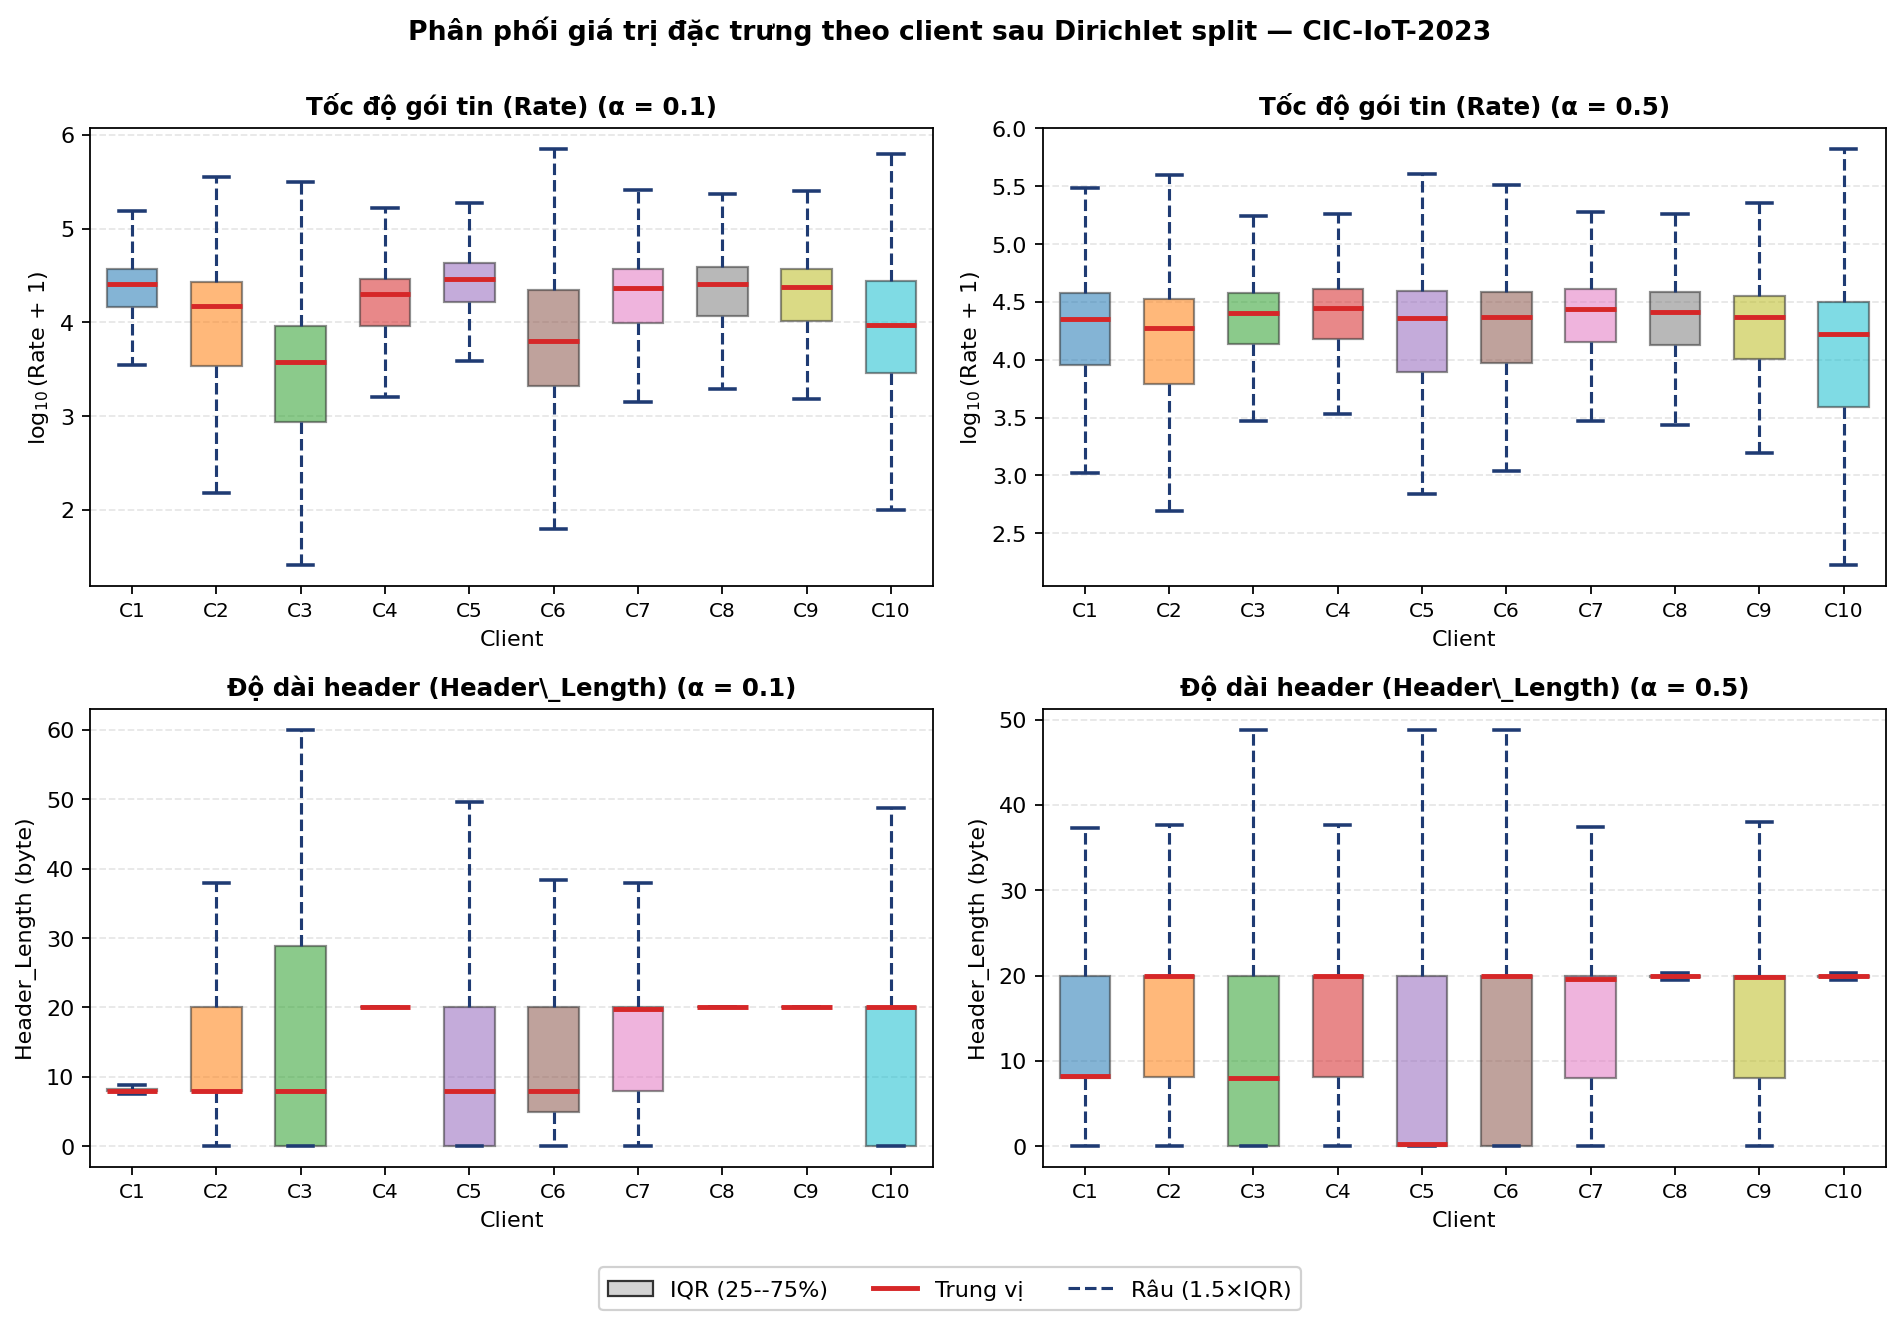
\includegraphics[width=0.95\linewidth]{Figures/fig_5_5_cic_iot_feature_skew_per_client.png}
    \caption{Phân phối giá trị đặc trưng theo client sau Dirichlet split -- CIC-IoT-2023 (\texttt{Rate} log-scale và \texttt{Header\_Length}; trái: $\alpha=0{,}1$, phải: $\alpha=0{,}5$)}
    \label{fig:cic_iot_feat_skew}
\end{figure}

\begin{figure}[H]
    \centering
    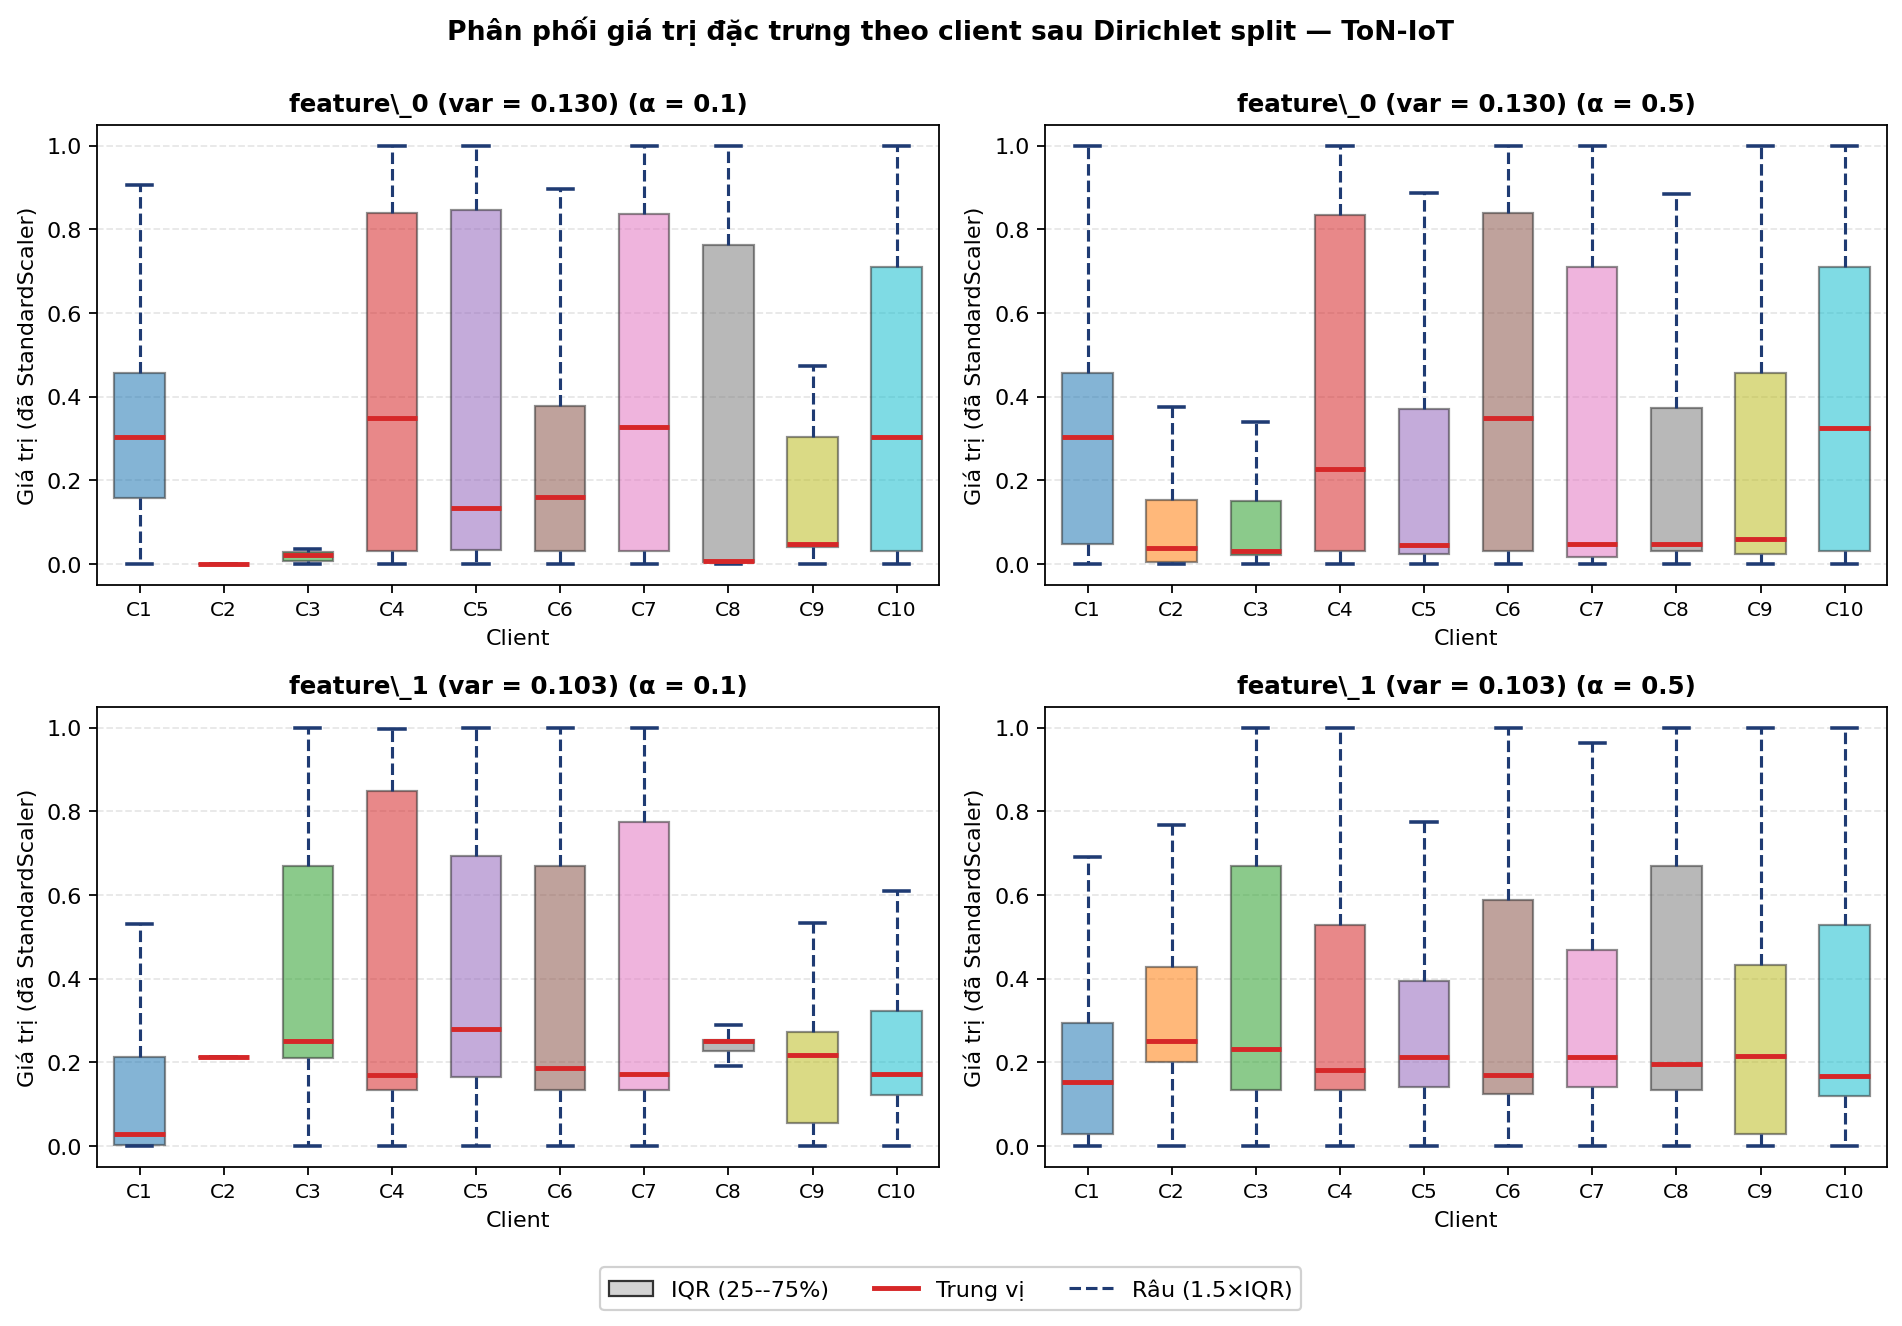
\includegraphics[width=0.95\linewidth]{Figures/fig_5_6_ton_iot_feature_skew_per_client.png}
    \caption{Phân phối giá trị đặc trưng theo client sau Dirichlet split -- ToN-IoT (\texttt{feature\_0} và \texttt{feature\_1}, hai cột có phương sai cao nhất sau StandardScaler; trái: $\alpha=0{,}1$, phải: $\alpha=0{,}5$)}
    \label{fig:ton_iot_feat_skew}
\end{figure}

Tóm lại, phân tích EDA cho thấy bốn đặc điểm quan trọng ảnh hưởng đến thực nghiệm: (1) cả hai dataset có mất cân bằng lớp nghiêm trọng, đòi hỏi Weighted Cross-Entropy Loss; (2) phân phối đặc trưng có nhiều outlier và nhiều bậc giá trị, ảnh hưởng đến chất lượng sinh dữ liệu của TabDDPM; (3) khi phân chia Dirichlet với $\alpha=0{,}1$, label skew trở nên cực đoan; (4) đồng thời feature skew cũng xuất hiện rõ rệt giữa các client. Hai dạng skew sau là nguyên nhân chính khiến các phương pháp phòng thủ thụ động nhầm client lành tính thành độc hại (Gap~2).

\section{Kịch bản A: Đánh giá hiệu năng phòng thủ}
Kịch bản A đánh giá hiệu năng phòng thủ của DT-Guard trên \textbf{hai bộ dữ liệu} (CIC-IoT-2023 và ToN-IoT) với \textbf{bốn mức tỉ lệ client độc hại} (10\%, 20\%, 40\%, 50\%), tổng cộng 5 tấn công $\times$ 4 tỉ lệ $\times$ 2 dataset = 40 kịch bản.

\subsection{Kết quả trên CIC-IoT-2023}
CIC-IoT-2023 có 39 đặc trưng và 34 lớp phân loại, được coi là kịch bản khó nhất trong hai dataset. Phần này phân tích kết quả qua hai hình minh chứng chính: \textbf{Hình 5.7} cho cặp Accuracy + Detection Rate và \textbf{Hình 5.8} cho heatmap FPR

\begin{figure}[H]
    \centering
    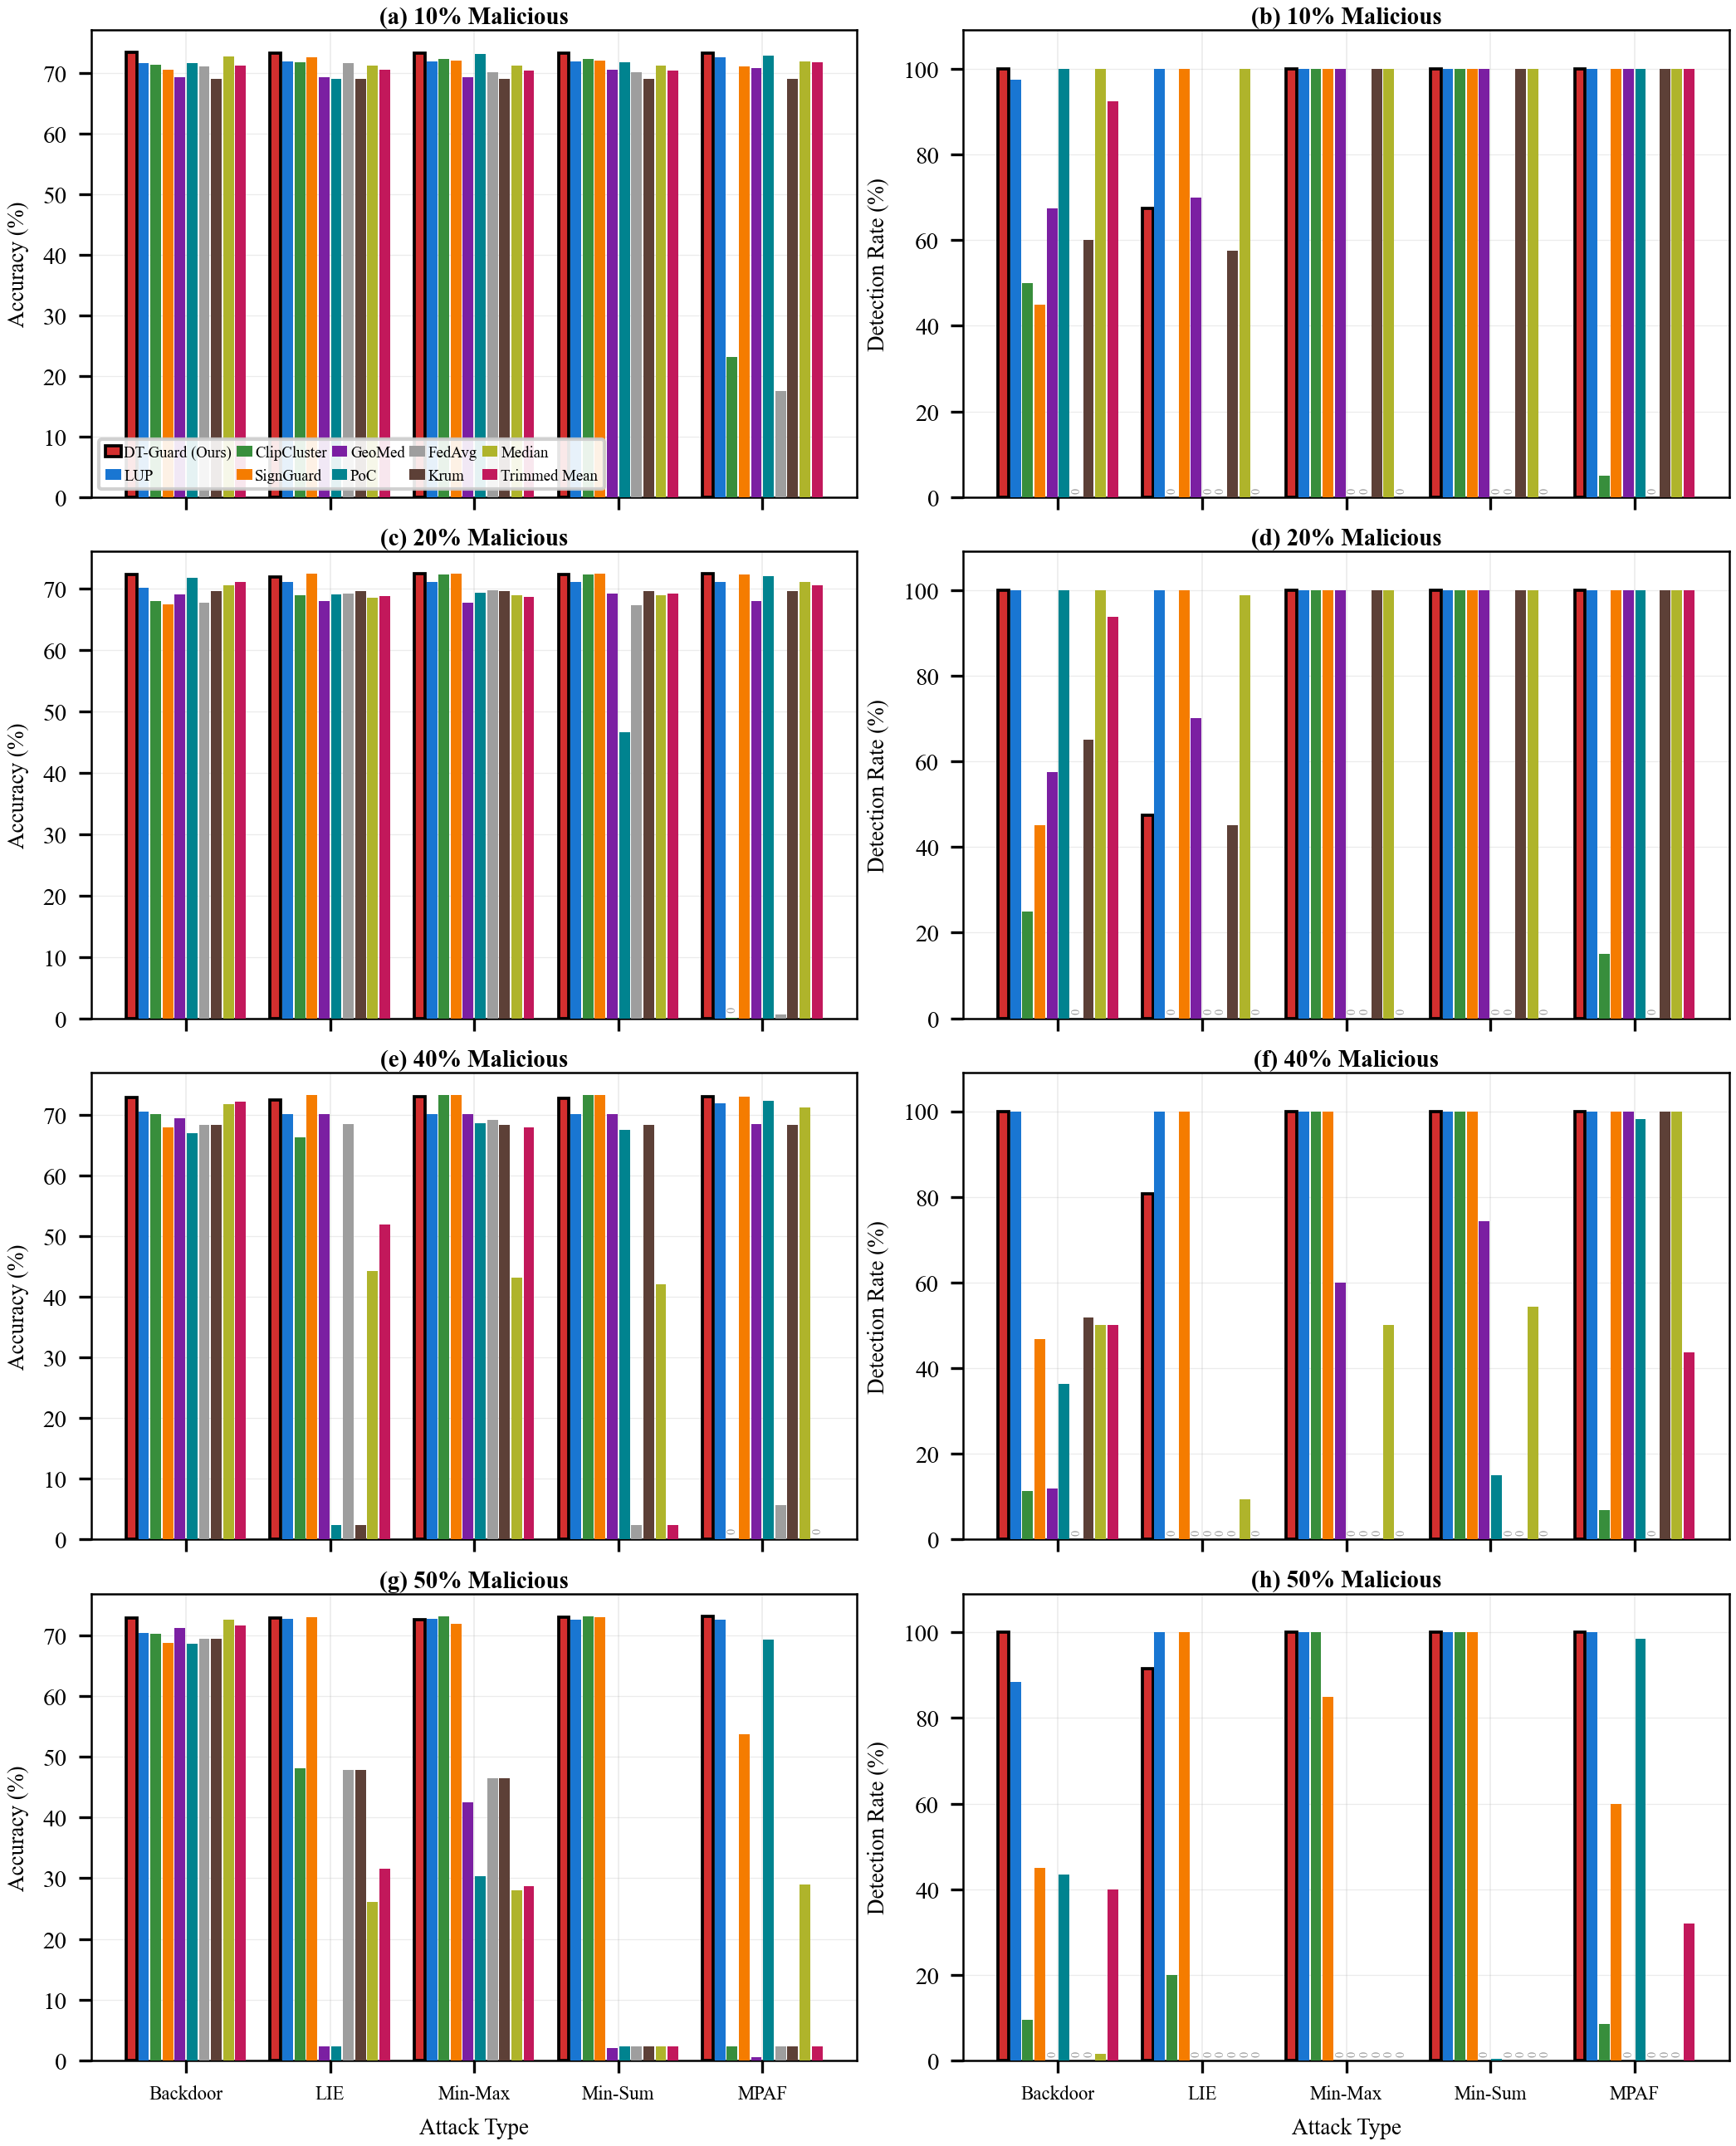
\includegraphics[width=0.85\linewidth]{Figures/fig_5_7_accuracy_dr_cic_iot_2023.png}
    \caption{Accuracy và Detection Rate trên CIC-IoT-2023 theo 4 mức tỉ lệ malicious}
\end{figure}

\textbf{Mỗi cặp panel ghép Accuracy của 10 phương pháp phòng thủ với Detection Rate tương ứng của DT-Guard trên 5 tấn công.}

\textbf{1)} DT-Guard giữ Accuracy ổn định bất chấp tỉ lệ tấn công. Bốn cột Accuracy của DT-Guard trong Hình 5.7 gần như cùng độ cao: trung bình 5 tấn công lần lượt là 73,26\% (10\%), 72,32\% (20\%), 72,74\% (40\%) và 72,84\% (50\%), biên độ dao động chưa đầy 1 điểm phần trăm. Khoảng {[}min, max{]} trên từng mức cũng rất hẹp: {[}73,19; 73,34{]}, {[}71,91; 72,49{]}, {[}72,40; 72,92{]} và {[}72,54; 73,09{]}. Điều này khẳng định pipeline kiểm chứng hành vi loại bỏ thành công bản cập nhật độc hại trước khi tổng hợp, mô hình toàn cục không bị "kéo lệch" dù tỉ lệ malicious tăng từ 10\% lên 50\%.

\textbf{2)} Detection Rate tăng dần khi tỉ lệ malicious tăng. Quan sát panel Detection Rate ở Hình 5.7, thanh DR trung bình của DT-Guard đi lên theo ratio: 93,5\% $\rightarrow$ 89,5\% $\rightarrow$ 96,1\% $\rightarrow$ 98,3\%. Tại mức 50\%, DT-Guard đạt 100\% trên Backdoor, Min-Max, Min-Sum, MPAF và 91,5\% trên LIE. Xu hướng tăng được giải thích như sau: khi nhiều attacker hơn, ảnh hưởng tập thể của các bản cập nhật độc hại trên không gian đặc trưng 39 chiều rõ rệt hơn, tạo sự phân biệt sắc nét hơn giữa hành vi suy luận lành tính và đầu độc trên challenge data. Riêng tấn công LIE có DR thấp nhất (67,5\% $\rightarrow$ 47,5\% $\rightarrow$ 80,6\% $\rightarrow$ 91,5\%) do biên độ nhiễu rất nhỏ, khó phân biệt khi số attacker còn ít. Điểm "lõm" tại 20\% (DR trung bình 89,5\%) hoàn toàn do LIE ở 20\% chỉ đạt 47,5\% kéo xuống, bốn tấn công còn lại vẫn 100\%.

\textbf{3)} Các baseline thất bại theo cơ chế cấu trúc, ngay cả ở mức malicious thấp. Đọc các nhóm cột trong panel Accuracy của Hình 5.7 từ trái sang phải:

\begin{itemize}
\item
  Nhóm không phòng thủ (FedAvg): Accuracy trung bình giảm theo ratio: 60,05\% (10\%) $\rightarrow$ 54,93\% (20\%) $\rightarrow$ 42,78\% (40\%) $\rightarrow$ 33,66\% (50\%). MPAF làm sụp FedAvg ở mọi ratio (17,49\% / 0,56\% / 5,67\% / 2,33\%) vì các fake clients chiếm đa số trọng số khi đơn thuần lấy trung bình. Min-Sum cũng kéo FedAvg xuống còn 2,33\% ở 40--50\% malicious.
\item
  Nhóm thống kê cổ điển (Krum, Median, Trimmed Mean, GeoMed): Cả bốn phương pháp này sụp nặng ở 50\% malicious: trung bình lần lượt 33,66\% (Krum), 31,61\% (Median), 27,29\% (Trimmed Mean), 23,76\% (GeoMed). Đặc biệt:

  \begin{itemize}
  \item
    Krum thất bại trước LIE (47,84\%) và sụp hoàn toàn trên Min-Sum, MPAF (cùng 2,33\%) vì các bản cập nhật độc hại tinh vi nằm ở giữa phân phối nên Krum chọn trúng chính chúng.
  \item
    Median sụp dưới Min-Sum (2,33\%), LIE (26,05\%), Min-Max (28,08\%), khi \textgreater50\% client là độc hại theo từng chiều, trung vị bị ảnh hưởng trực tiếp.
  \item
    Trimmed Mean sụp dưới Min-Sum (2,33\%) và MPAF (2,33\%); cắt outlier theo L2 norm không có tác dụng khi attack nằm trong phân phối lành tính.
  \item
    GeoMed sụp dưới LIE (2,33\%), Min-Sum (2,12\%), MPAF (0,60\%), geometric median bị kéo về cụm độc hại khi tỷ lệ tấn công lớn.
  \end{itemize}
\item
  Nhóm phân tích nâng cao (SignGuard, ClipCluster, LUP, PoC): Ba phương pháp đầu duy trì accuracy khá hơn nhưng vẫn có lỗ hổng đặc trưng:

  \begin{itemize}
  \item
    SignGuard sụp dưới MPAF (53,68\% ở 50\%) vì các fake clients có hướng dấu gradient đồng nhất, lọt qua bộ lọc dấu.
  \item
    ClipCluster sụp dưới MPAF ở mọi ratio (23,13\% $\rightarrow$ 0,05\% $\rightarrow$ 0,05\% $\rightarrow$ 2,33\%) vì các fake clients tạo cụm đông nhất, ClipCluster chọn nhầm cụm độc hại.
  \item
    LUP giữ accuracy cao nhất nhóm baseline (72,16\% trung bình ở 50\% malicious) nhưng phải đánh đổi bằng FPR rất cao (xem phần Phân tích False Positive Rate bên dưới).
  \item
    PoC sụp dưới LIE và Min-Sum ở 40--50\% (cùng 2,33\%) vì MMD đo khoảng cách tham số không phân biệt được Non-IID tự nhiên với đầu độc tinh vi.
  \end{itemize}
\end{itemize}

\begin{figure}[H]
    \centering
    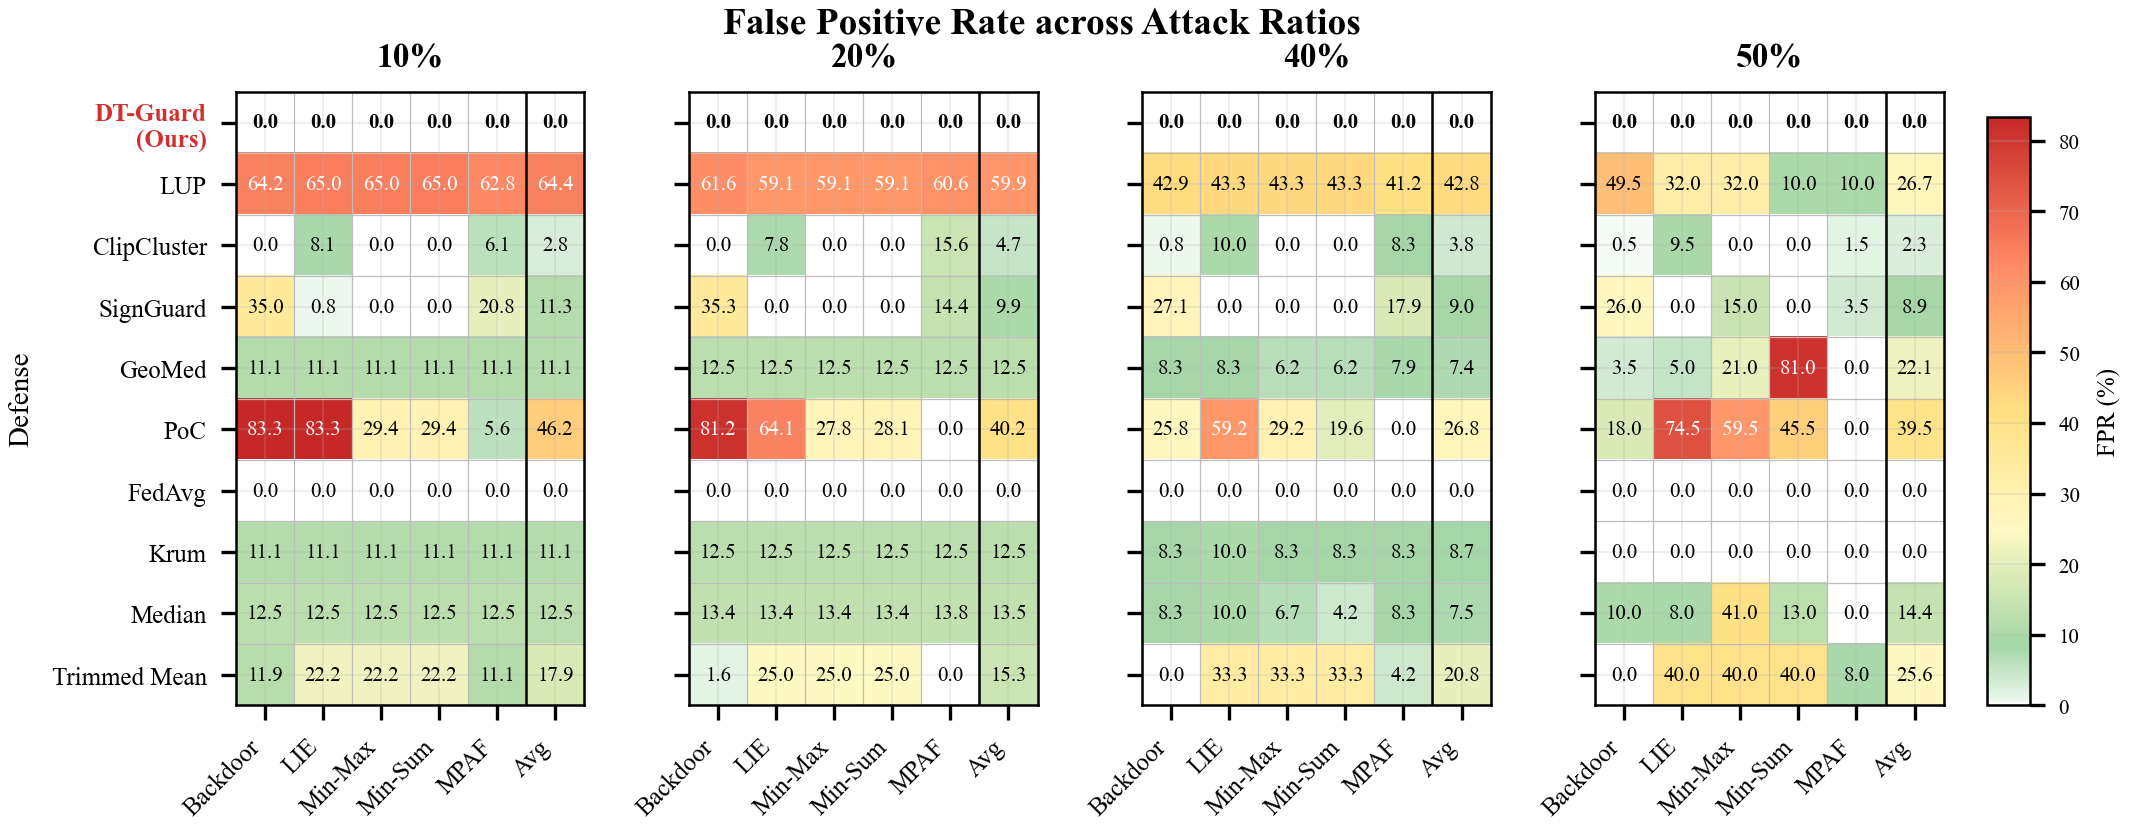
\includegraphics[width=0.85\linewidth]{Figures/fig_5_8_fpr_cic_iot_2023.png}
    \caption{Heatmap False Positive Rate (FPR) trên CIC-IoT-2023 theo 4 mức tỉ lệ malicious}
\end{figure}

\textbf{Mỗi ô là tỷ lệ client lành tính bị loại nhầm ở một cặp (defense, attack); ô càng đậm đỏ càng nhiều client bị loại oan.}

\textbf{Phân tích False Positive Rate (Hình 5.8)}

\textbf{1)} DT-Guard duy trì hàng FPR = 0\% xuyên suốt 20 ô (5 tấn công $\times$ 4 ratio). Hàng DT-Guard trong Hình 5.8 hoàn toàn trắng, không một client lành tính nào bị loại nhầm trong toàn bộ thực nghiệm trên CIC-IoT-2023. Đây là minh chứng trực tiếp cho luận điểm "kiểm chứng hành vi chủ động" của DT-Guard: bằng cách đo F1 trên challenge data thay vì so khoảng cách tham số, các client Non-IID lành tính vẫn vượt qua được Trust-Gate.

\textbf{2)} Hàng LUP có FPR cao bất thường, minh chứng cho Gap 2 (Non-IID confusion). LUP có FPR trung bình 64,39\% (10\%) $\rightarrow$ 59,87\% (20\%) $\rightarrow$ 42,83\% (40\%) $\rightarrow$ 26,70\% (50\%); riêng cell (LUP, Backdoor ở mức 10\%) đạt 65,00\%. Nghĩa là hơn nửa client lành tính bị MAD và hierarchical clustering của LUP đánh nhầm là outlier trong phần lớn kịch bản. Đây chính là điểm yếu cốt lõi của các phương pháp phân tích tham số thụ động khi gặp dữ liệu Non-IID nghiêm trọng.

\textbf{3)} Hàng PoC cũng có FPR rất cao (46,22\% $\rightarrow$ 40,25\% $\rightarrow$ 26,75\% $\rightarrow$ 39,50\% trung bình; đỉnh 83,33\% ở 10\% malicious). MMD đo khoảng cách phân phối tham số gặp đúng vấn đề như LUP.

\textbf{4)} Các baseline thống kê có FPR thấp hơn nhưng không "miễn phí". Krum, Median, GeoMed, Trimmed Mean có FPR trong khoảng 7--25\% trung bình, thấp hơn LUP/PoC nhưng vẫn loại nhầm 1--4 client lành tính mỗi vòng. Đáng chú ý: Krum ở mức 50\% có FPR = 0\% nhưng đó là vì nó \textbf{chọn duy nhất 1 client} mỗi vòng (không có khái niệm "loại nhầm"), đồng thời chính nó sụp accuracy còn 33,66\%. FedAvg cũng có FPR = 0\% chỉ vì không có cơ chế loại bỏ nào.

\textbf{Tổng kết cho CIC-IoT-2023}

Trên dataset khó nhất (39 đặc trưng, 34 lớp), DT-Guard cho thấy ba kết quả nhất quán: \textbf{(1)} Accuracy ổn định \textasciitilde73\% bất chấp tỉ lệ tấn công tăng 5 lần (10\% $\rightarrow$ 50\%); \textbf{(2)} Detection Rate trung bình tăng dần từ 89,5\% lên 98,3\% và đạt 100\% trên 4/5 tấn công ở mức malicious cao nhất; \textbf{(3)} FPR = 0\% trên toàn bộ 20 kịch bản. Trong khi đó, mọi baseline thuộc nhóm phân tích tham số thụ động đều bộc lộ lỗ hổng cấu trúc trước ít nhất một loại tấn công, hoặc phải đánh đổi accuracy bằng FPR cao (LUP, PoC), hoặc sụp accuracy nghiêm trọng (FedAvg, Krum, Median, Trimmed Mean, GeoMed) khi tỉ lệ malicious vượt 40\%.

\subsection{Kết quả trên ToN-IoT}
ToN-IoT có 10 đặc trưng và 10 lớp phân loại, không gian đặc trưng nhỏ hơn nhiều so với CIC-IoT-2023. Phần này áp dụng cùng bố cục phân tích: \textbf{Hình 5.9} cho cặp Accuracy + Detection Rate và \textbf{Hình 5.10} cho heatmap FPR

\begin{figure}[H]
    \centering
    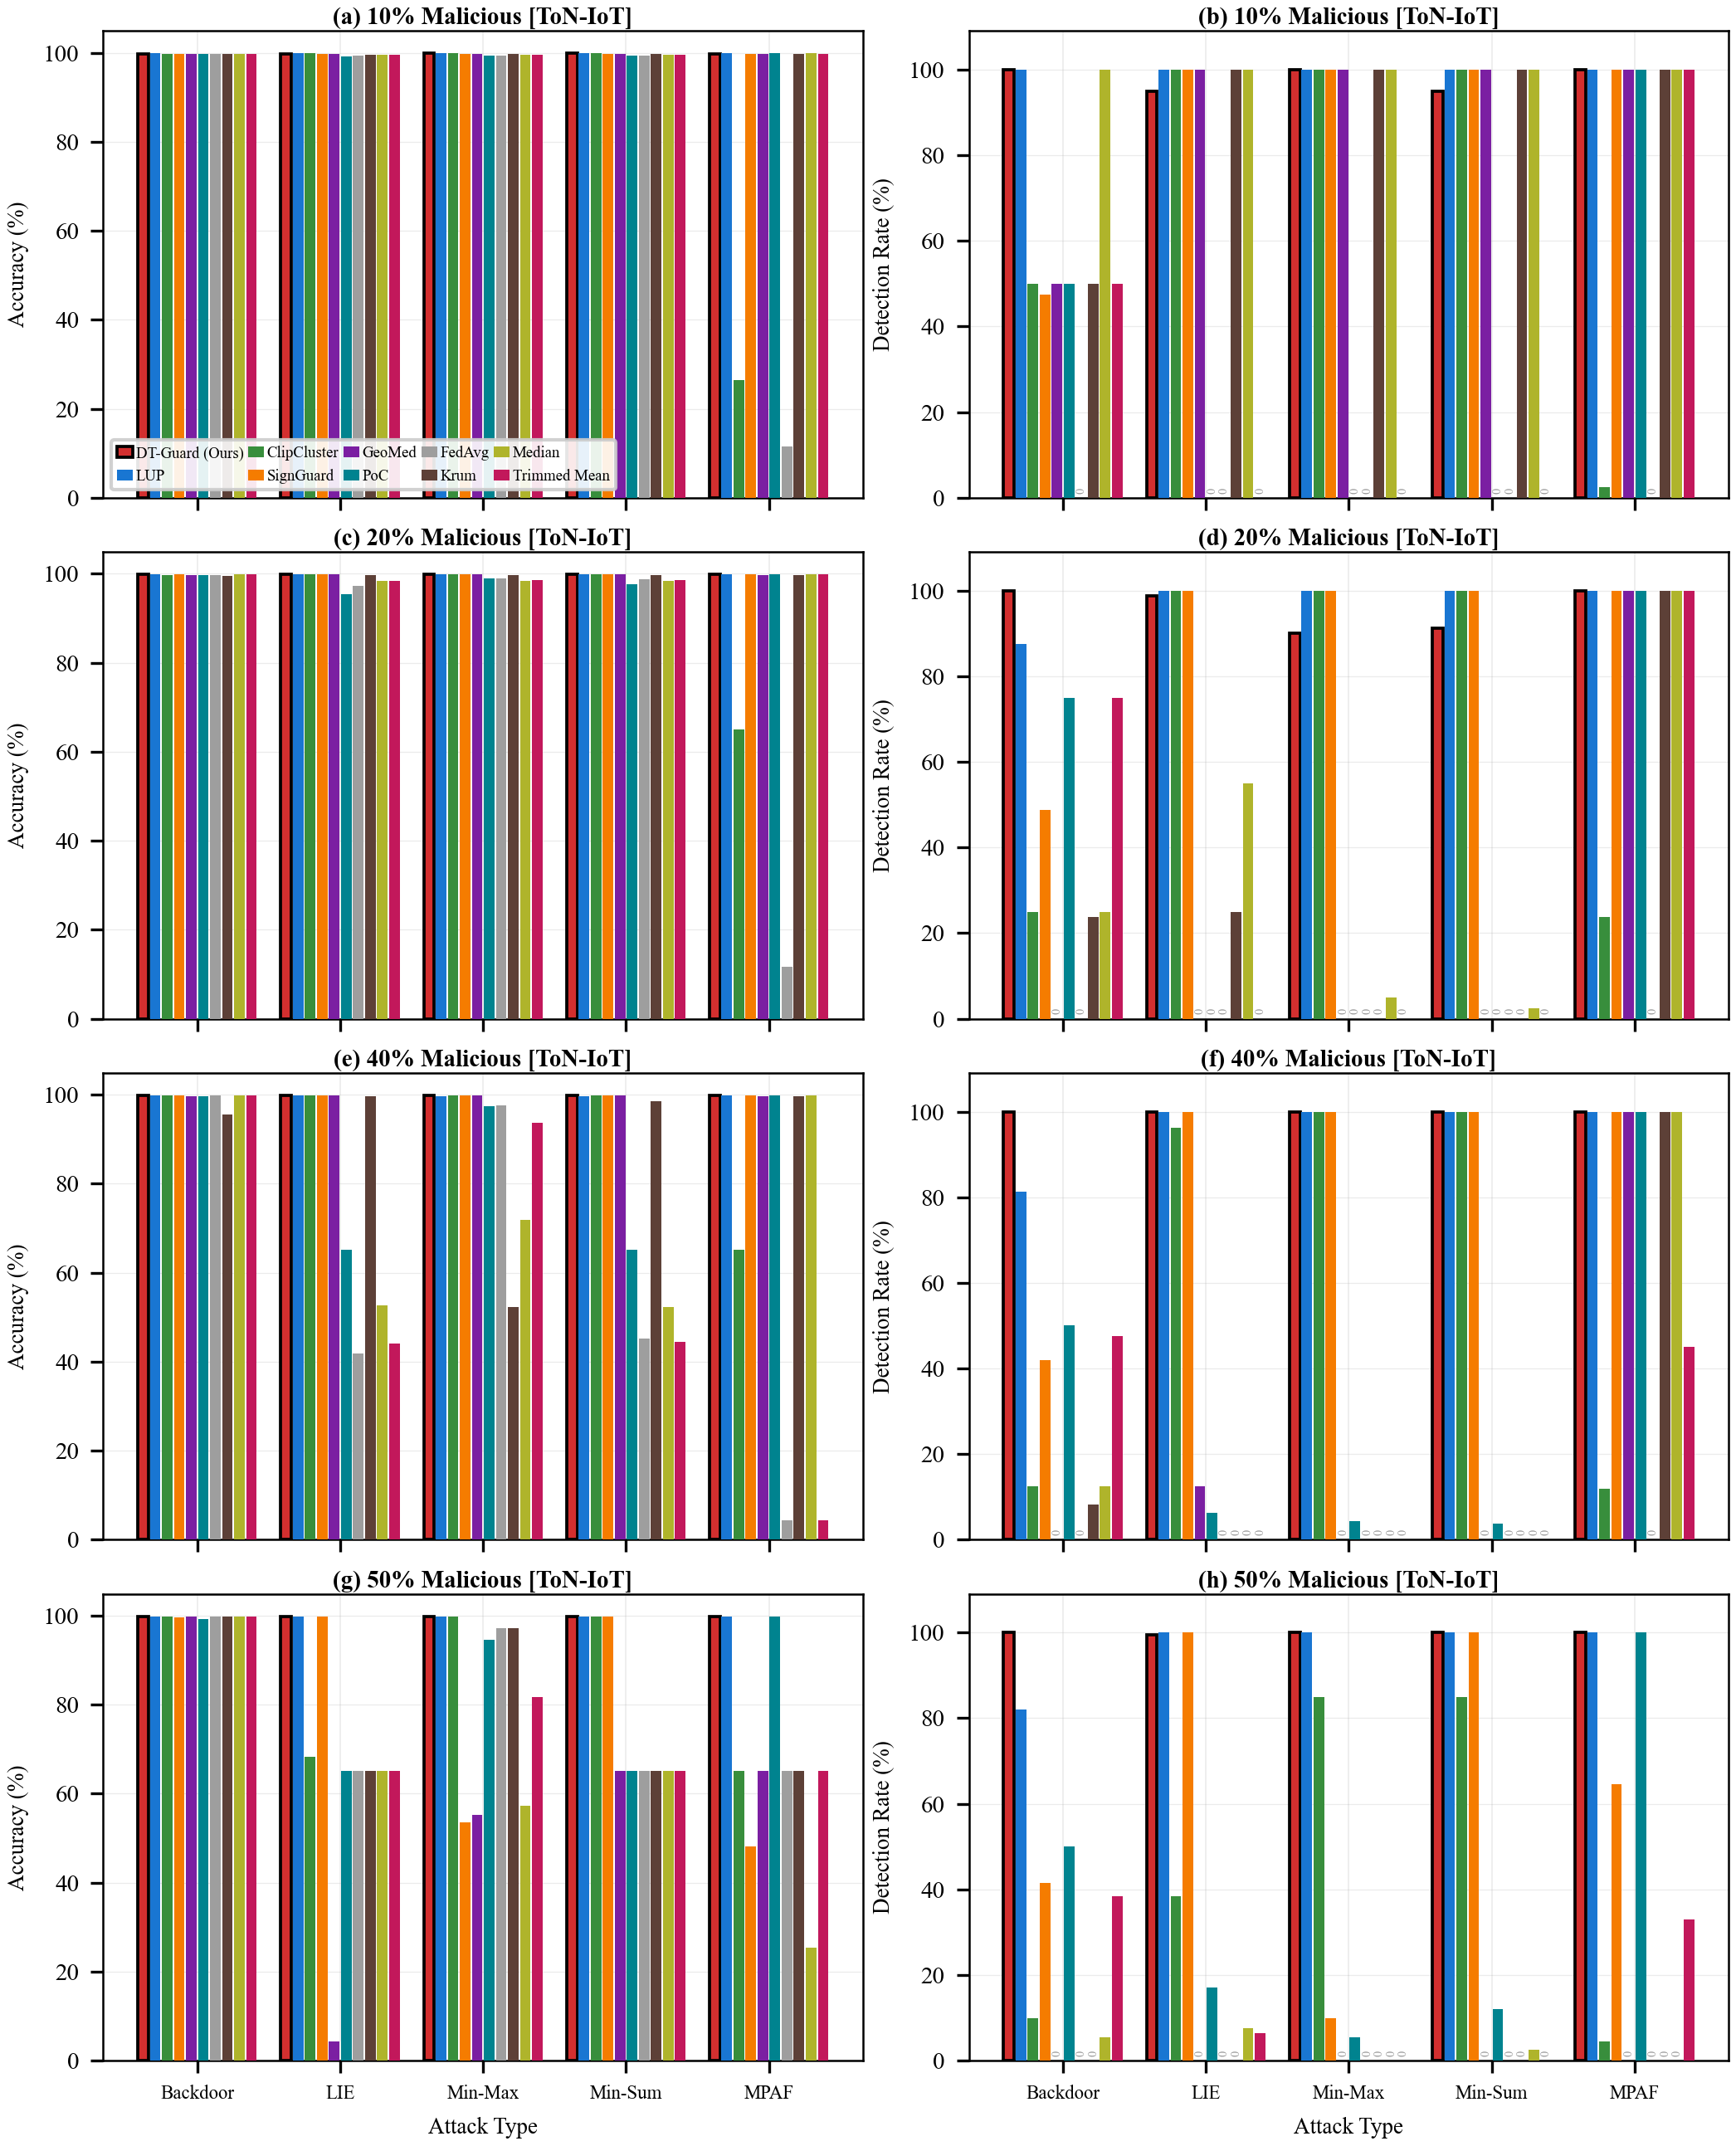
\includegraphics[width=0.85\linewidth]{Figures/fig_5_9_accuracy_dr_ton_iot.png}
    \caption{Accuracy và Detection Rate trên ToN-IoT theo 4 mức tỉ lệ malicious}
\end{figure}

\textbf{Mỗi cặp panel ghép Accuracy của 10 phương pháp phòng thủ với Detection Rate tương ứng của DT-Guard trên 5 tấn công.}

\textbf{Hiệu năng phát hiện xâm nhập (Hình 5.9), Accuracy và Detection Rate}

\textbf{1)} DT-Guard đạt accuracy gần như hoàn hảo và bất biến theo ratio. Bốn cột Accuracy của DT-Guard ở Hình 5.9 cùng cao đến mức gần trần: 99,81\% (10\%) $\rightarrow$ 99,80\% (20\%) $\rightarrow$ 99,84\% (40\%) $\rightarrow$ 99,83\% (50\%). Khoảng {[}min, max{]} cũng cực hẹp: {[}99,80; 99,83{]}, {[}99,78; 99,82{]}, {[}99,82; 99,86{]}, {[}99,81; 99,84{]}. So sánh với CIC-IoT-2023 (\textasciitilde73\%), accuracy cao hơn \textasciitilde27 điểm phần trăm phản ánh độ phức tạp bài toán: ToN-IoT chỉ có 10 lớp/10 đặc trưng nên kiến trúc MLP (256 $\rightarrow$ 128 $\rightarrow$ 64) đủ năng lực biểu diễn ranh giới phân loại; mất cân bằng lớp cũng nhẹ hơn (lớp lành tính chiếm \textasciitilde52\%).

\textbf{2)} Detection Rate đạt mức gần hoàn hảo ở ratio cao. Theo dõi panel Detection Rate ở Hình 5.9:

\begin{itemize}
\item
  \textbf{10\% malicious:} DT-Guard đạt 100\% trên Backdoor, Min-Max, MPAF; 95,0\% trên LIE và Min-Sum (DR trung bình 98,0\%).
\item
  \textbf{20\% malicious:} 100\% trên Backdoor và MPAF; 98,75\% trên LIE; 91,25\% trên Min-Sum; 90,0\% trên Min-Max (DR trung bình 96,0\%).
\item
  \textbf{40\% malicious:} \textbf{100\% trên cả 5 tấn công}, DT-Guard phát hiện toàn bộ attacker dù gần một nửa client là độc hại.
\item
  \textbf{50\% malicious:} 100\% trên Backdoor, Min-Max, Min-Sum, MPAF; 99,5\% trên LIE (DR trung bình 99,9\%).
\end{itemize}

So với CIC-IoT-2023 (LIE ở mức 50\% chỉ đạt 91,5\%), DR trên ToN-IoT vượt trội: ngay cả LIE, tấn công khó phát hiện nhất, cũng đạt 99,5\%. Nguyên nhân: trong không gian đặc trưng 10 chiều, mỗi chiều tham số có ảnh hưởng lớn hơn đến kết quả phân loại, do đó cùng một biên độ nhiễu của LIE tạo ra sai lệch hành vi rõ rệt hơn trên challenge data. Sự giảm nhẹ ở mức 20\% (DR Min-Max và Min-Sum giảm còn 90\% và 91,25\%) là do số attacker vẫn ít (4 client), chưa tạo được "đa số phá hoại" rõ rệt.

\textbf{3)} Các baseline thất bại theo đúng cơ chế đã quan sát trên CIC-IoT-2023. Đọc panel Accuracy ở Hình 5.9, ngay cả khi accuracy nền của ToN-IoT cao hơn nhiều, các baseline vẫn sụp đổ ở 50\% malicious:

\begin{itemize}
\item
  FedAvg sụp đồng loạt dưới LIE, Min-Sum và MPAF (cùng 65,07\%, tức về mức random guess) $\rightarrow$ trung bình 78,43\%.
\item
  Krum có pattern thất bại y hệt FedAvg (cùng 78,43\%, sụp dưới đúng 3 tấn công LIE/Min-Sum/MPAF cùng 65,07\%), minh chứng Krum không khác FedAvg khi tấn công lọt vào vùng trung tâm phân phối.
\item
  Median sụp dưới MPAF (25,48\%), LIE (65,07\%), Min-Max (57,34\%), Min-Sum (65,07\%) $\rightarrow$ trung bình 62,55\%.
\item
  Trimmed Mean sụp dưới LIE, Min-Sum, MPAF (cùng 65,07\%) $\rightarrow$ trung bình 75,36\%.
\item
  GeoMed sụp nặng nhất: LIE (4,34\%), Min-Max (55,14\%), Min-Sum (65,07\%), MPAF (65,07\%) $\rightarrow$ trung bình 57,86\% (thấp nhất nhóm).
\item
  ClipCluster sụp dưới LIE (68,19\%) và MPAF (65,07\%) $\rightarrow$ trung bình 86,53\%.
\item
  SignGuard sụp dưới Min-Max (53,53\%) và MPAF (48,17\%) $\rightarrow$ trung bình 80,18\%.
\item
  PoC sụp dưới LIE (65,07\%) và Min-Sum (65,07\%) $\rightarrow$ trung bình 84,75\%.
\item
  LUP là baseline duy nhất duy trì accuracy cao (99,84\% trung bình), nhưng phải đánh đổi bằng FPR cao (xem phần Phân tích False Positive Rate bên dưới).
\end{itemize}

\begin{figure}[H]
    \centering
    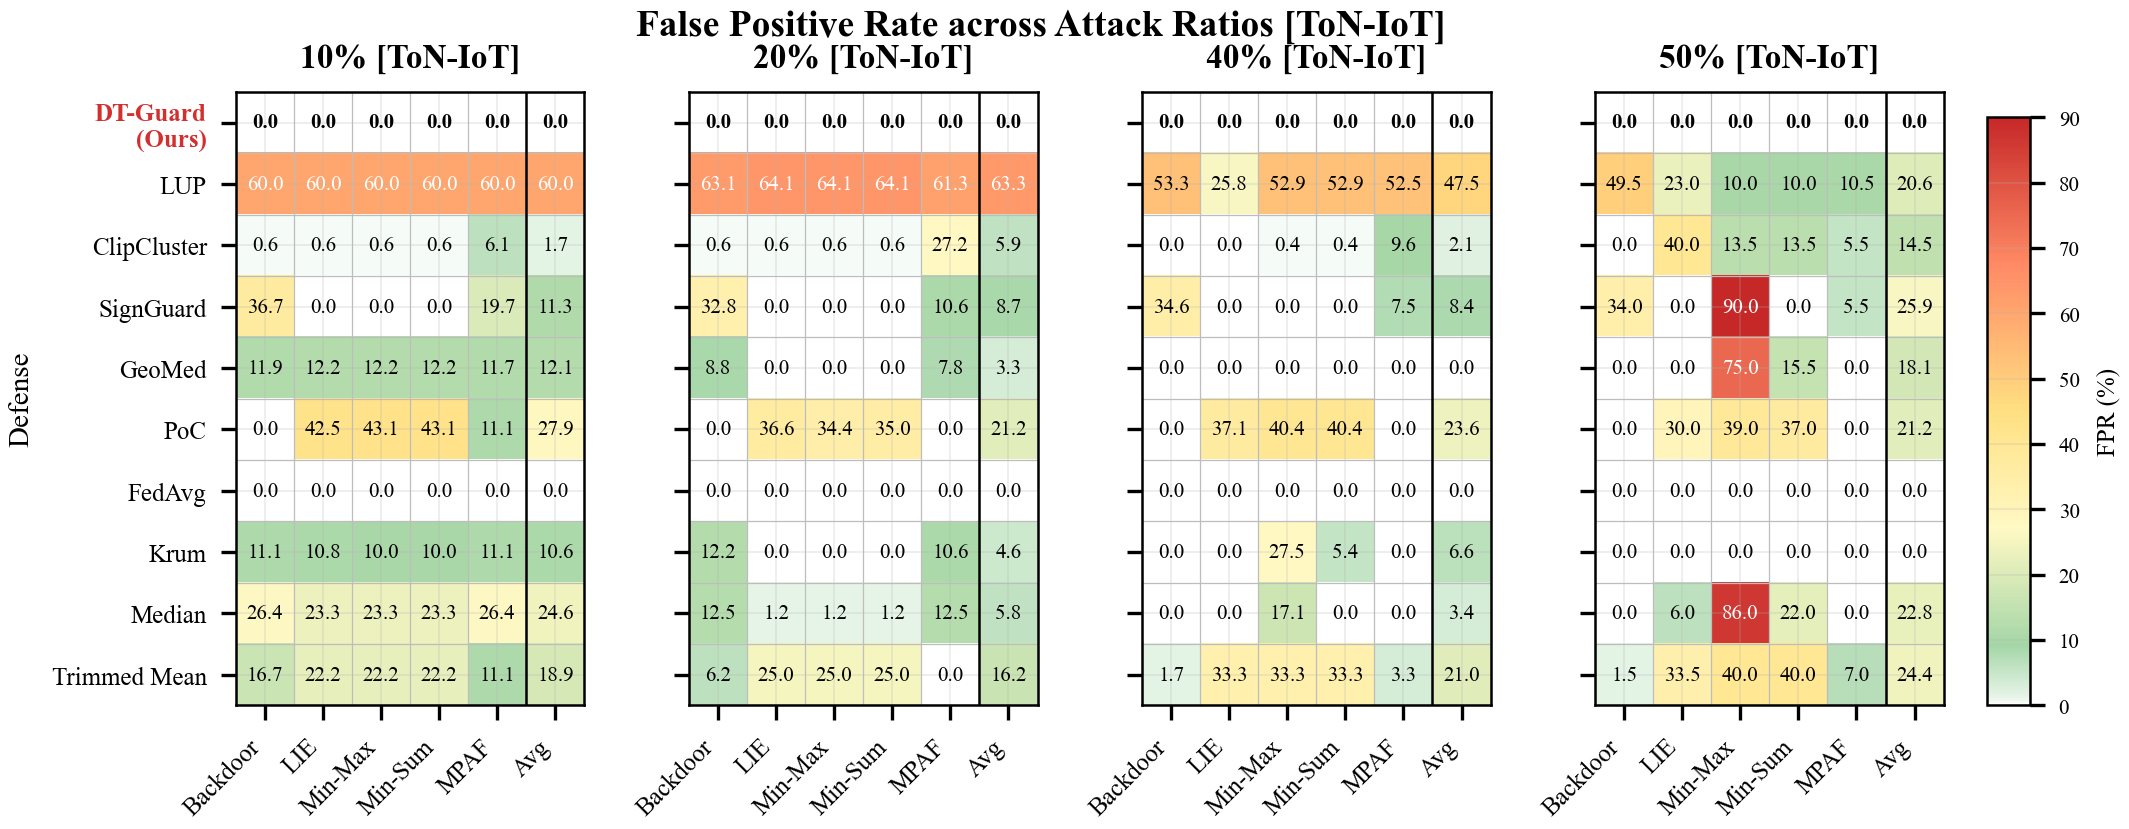
\includegraphics[width=0.85\linewidth]{Figures/fig_5_10_fpr_ton_iot.png}
    \caption{Heatmap False Positive Rate (FPR) trên ToN-IoT theo 4 mức tỉ lệ malicious}
\end{figure}

\textbf{Quan sát hàng DT-Guard hoàn toàn trắng so với hàng LUP, PoC, SignGuard có nhiều ô đỏ đậm.}

\textbf{Phân tích False Positive Rate (Hình 5.10)}

\textbf{1)} DT-Guard giữ FPR = 0\% xuyên suốt 20 ô. Hàng DT-Guard trong Hình 5.10 toàn trắng, kết quả nhất quán với CIC-IoT-2023 (Hình 5.8). Điều này xác nhận nguyên lý kiểm chứng hành vi không phụ thuộc kích thước không gian đặc trưng: client Non-IID lành tính ở cả 10 chiều và 39 chiều đều phân loại chính xác trên challenge data.

\textbf{2)} LUP có FPR rất cao ở mọi ratio. FPR trung bình của LUP: 60,00\% (10\%) $\rightarrow$ 63,31\% (20\%) $\rightarrow$ 47,50\% (40\%) $\rightarrow$ 20,60\% (50\%); đỉnh 64,06\% ở mức 20\% malicious. Mặc dù LUP giữ accuracy cao, mỗi vòng nó loại nhầm hơn nửa số client lành tính, minh chứng chính cho luận điểm "LUP thưởng cho các client trùng phân phối với mô hình toàn cục, đánh nhầm Non-IID lành tính là outlier."

\textbf{3)} Một số baseline có ô FPR rất đậm tại 50\% malicious. Đáng chú ý:

\begin{itemize}
\item
  SignGuard ở mức 50\%, Min-Max: FPR = 90,00\% (trung bình 25,90\%), chiều dấu gradient bị Min-Max thao túng đồng đều, SignGuard loại nhầm gần toàn bộ client lành tính.
\item
  Median ở mức 50\%, LIE: FPR = 86,00\% (trung bình 22,80\%), trung vị từng chiều bị "kéo" bởi cụm độc hại đồng nhất.
\item
  GeoMed ở mức 50\%, LIE: FPR = 75,00\% (trung bình 18,10\%).
\item
  PoC ổn định ở mức FPR cao 21--28\% trung bình qua mọi ratio.
\end{itemize}

\textbf{4)} Krum và FedAvg có FPR = 0\% nhưng đó không phải là điểm cộng. Krum chỉ chọn 1 client/vòng (không có khái niệm loại nhầm), FedAvg không có cơ chế lọc, cả hai đều phải trả giá bằng accuracy thấp như đã phân tích ở phần Hiệu năng phát hiện xâm nhập.

\textbf{Tổng kết cho ToN-IoT}

Trên dataset đơn giản hơn (10 đặc trưng, 10 lớp), DT-Guard cho ba kết quả mạnh hơn cả trên CIC-IoT-2023: \textbf{(1)} Accuracy $\approx$ 99,8\% bất biến qua 4 ratio; \textbf{(2)} Detection Rate đạt 100\% trên cả 5 tấn công ngay từ ratio 40\% và duy trì 99,9\% ở 50\%; \textbf{(3)} FPR = 0\% trên toàn bộ 20 kịch bản. Cùng các baseline cũng dễ phòng thủ hơn ở ratio thấp (\textasciitilde99\% accuracy ở 10--20\%) nhưng vẫn sụp đổ ở 50\% malicious theo đúng cơ chế thất bại đã quan sát trên CIC-IoT-2023, tái xác nhận tính cấu trúc (chứ không phải tham số) của lỗ hổng.

\subsection{So sánh chéo giữa hai dataset}
Việc đánh giá trên hai dataset khác biệt hoàn toàn, CIC-IoT-2023 (34 lớp, 39 đặc trưng, IoTAttackNet/MLP) và ToN-IoT (10 lớp, 10 đặc trưng, MLP), cho phép rút ra kết luận quan trọng về tính tổng quát hóa của cả phương pháp đề xuất lẫn các baseline.

\textbf{Sự nhất quán của DT-Guard trên cả hai dataset:} Cả CIC-IoT-2023 và ToN-IoT đều cho thấy ba đặc trưng ổn định: (1) accuracy duy trì ổn định qua mọi mức malicious; (2) Detection Rate cao và tăng dần khi tỉ lệ malicious tăng; (3) FPR = 0,0\% trên tất cả kịch bản. Nguyên lý kiểm chứng hành vi hoạt động hiệu quả bất kể kích thước không gian đặc trưng (39 vs. 10), số lớp phân loại (34 vs. 10), hay mức độ mất cân bằng lớp, vì pipeline đánh giá trực tiếp năng lực phân loại trên challenge data chứ không phụ thuộc vào đặc trưng cụ thể của dataset.

\textbf{Sự nhất quán trong cơ chế thất bại của baseline:} ClipCluster luôn sụp dưới MPAF, GeoMed luôn sụp dưới LIE, SignGuard luôn sụp dưới Min-Max và Min-Sum, bất kể dataset nào. Điều này chứng tỏ lỗ hổng của nhóm phương pháp chỉ phân tích đặc trưng tĩnh của tham số là \textbf{cấu trúc}, không phải do tham số tinh chỉnh kém, không phải do đặc thù dataset, mà do bản thân cách tiếp cận thụ động không thể phân biệt giữa tham số bình thường và tham số bị đầu độc tinh vi. Việc cùng một phương pháp thất bại trước cùng loại tấn công ở cả hai môi trường thử nghiệm cho thấy lỗ hổng là cố hữu trong thiết kế, không phụ thuộc ngữ cảnh.

\textbf{Điểm khác biệt đáng chú ý giữa hai dataset:} Trên ToN-IoT, DR đạt 100\% ở mọi tấn công ngay từ mức 40\% malicious, trong khi trên CIC-IoT-2023, cần đến 50\% malicious mới đạt 98,3\%. Accuracy trên ToN-IoT (99,83\%) cũng cao hơn đáng kể so với CIC-IoT-2023 (72,8\%). Sự khác biệt này phản ánh mức độ khó của bài toán phân loại chứ không phải hiệu năng của DT-Guard, ToN-IoT có 10 lớp và 10 đặc trưng nên mô hình phân loại chính xác hơn và các dấu hiệu đầu độc cũng dễ phát hiện hơn trong không gian nhỏ. Kết quả này cho thấy DT-Guard hiệu quả hơn trên các bài toán có không gian đặc trưng nhỏ, nhưng vẫn bảo vệ đầy đủ trên bài toán phức tạp hơn (CIC-IoT-2023) mà không có sự suy giảm nghiêm trọng nào.

DT-Guard khắc phục được lỗ hổng cấu trúc của các phương pháp thụ động nhờ đánh giá hành vi suy luận thực tế, nguyên lý này tổng quát, không phụ thuộc vào đặc trưng dataset hay kiến trúc mô hình IDS.

\subsection{Giải thích hiện tượng đặc biệt}
\textbf{Hiện tượng 1:} DR tăng khi tỉ lệ malicious tăng. Đây là một xu hướng thoạt nhìn có vẻ phản trực giác: càng nhiều client độc hại thì lại càng dễ phát hiện. Nguyên nhân nằm ở cơ chế tổng hợp FedAvg: khi tỉ lệ malicious tăng, tổng trọng số của các bản cập nhật độc hại trong mô hình toàn cục cũng tăng theo. Mô hình toàn cục bị nhiễu nhiều hơn, khiến mô hình cục bộ của client lành tính (không bị đầu độc) có hành vi phân loại ngày càng khác biệt so với mô hình toàn cục trên challenge data. Khoảng cách hành vi này tạo ra sự phân tách rõ nét hơn trong Trust-Score, client độc hại có F1 thấp trên challenge data trong khi client lành tính vẫn phân loại chính xác. Hơn nữa, khi số lượng attacker lớn hơn, pattern đầu độc cũng đồng nhất hơn (các attacker cùng thực hiện một chiến thuật), tạo ra cụm hành vi đặc trưng dễ nhận diện hơn so với khi chỉ có 1--2 attacker bị chìm giữa nhiều client lành tính.

Cụ thể, trên CIC-IoT-2023: DR trung bình tăng từ 93,5\% (10\%) $\rightarrow$ 89,5\% (20\%) $\rightarrow$ 96,1\% (40\%) $\rightarrow$ 98,3\% (50\%). Ngoại lệ nhỏ ở mức 20\% (89,5\% thấp hơn 93,5\% ở mức 10\%) là do ở tỉ lệ này, LIE attack chỉ đạt DR 47,5\%, mức thấp nhất kéo trung bình xuống. Ở 10\% malicious (2 client độc hại), LIE được phát hiện 67,5\% nhờ vào 2 attacker này tạo ra một sự khác biệt vừa đủ trong hành vi. Nhưng khi tăng lên 20\% (4 attacker), LIE vẫn thay đổi rất ít tham số và 4 attacker chưa đủ tạo ra pattern rõ ràng, nên DR giảm tạm thời. Khi vượt qua ngưỡng 40\% (8 attacker), ảnh hưởng tập thể đủ mạnh để pipeline nhận diện.

\textbf{Hiện tượng 2:} LIE là tấn công khó phát hiện nhất. Trên cả hai dataset, LIE luôn có DR thấp nhất trong 5 tấn công (67,5\% tại 10\% malicious trên CIC-IoT-2023, và cũng là tấn công cuối cùng đạt 100\% DR trên ToN-IoT). Nguyên nhân gốc rễ nằm ở chiến lược thiết kế của LIE: thay đổi tham số "vừa đủ" để nằm trong vùng phân phối thống kê bình thường, cụ thể, attacker cộng thêm một lượng z $\times$ $\sigma$ vào giá trị trung bình mỗi chiều, với z được điều chỉnh cẩn thận. Lượng thay đổi này rất nhỏ so với các tấn công khác như MPAF (nhân bản update $\times10)$ hay Backdoor (thay đổi chuyên biệt 2 lớp cuối), nên hành vi suy luận của mô hình bị đầu độc cũng chỉ sai lệch nhẹ trên challenge data. Pipeline 4 lớp vẫn phát hiện được nhờ đánh giá trực tiếp F1 trên challenge data thay vì chỉ nhìn khoảng cách tham số, nhưng cần nhiều "bằng chứng" hơn (nhiều mẫu challenge, tỉ lệ malicious cao hơn) để phân biệt giữa sai lệch nhỏ ngẫu nhiên và sai lệch do đầu độc.

Tuy nhiên, kết quả quan trọng là: ngay cả với LIE, tấn công khó nhất, DT-Guard vẫn đạt DR 91,5\% tại 50\% malicious trên CIC-IoT-2023 và 99,5\% trên ToN-IoT. Điều này cho thấy pipeline kiểm chứng hành vi có khả năng chịu đựng ngay cả với các tấn công được thiết kế tinh vi nhất, miễn là tỉ lệ độc hại đủ cao để tạo ra dấu hiệu nhận diện.

\textbf{Hiện tượng 3:} Accuracy gần như không đổi khi tỉ lệ malicious tăng. Trên CIC-IoT-2023, accuracy dao động trong khoảng hẹp 72,3\%--73,3\% qua cả 4 mức tỉ lệ malicious; trên ToN-IoT, accuracy ổn định ở 99,80\%--99,84\%. Hiện tượng này cho thấy DT-Guard loại bỏ hiệu quả các bản cập nhật độc hại trước khi tổng hợp, chỉ các client vượt qua Trust Gate mới tham gia vào mô hình toàn cục. Kết quả là mô hình toàn cục không bị suy giảm dù tỉ lệ tấn công tăng từ 10\% lên 50\%. Tuy nhiên, accuracy không tăng khi tỉ lệ malicious giảm (từ 50\% xuống 10\%) vì accuracy chủ yếu bị giới hạn bởi khả năng phân loại của mô hình IDS trên bài toán 34 lớp (CIC-IoT-2023) chứ không phải bởi tấn công, tức là mô hình đã đạt "trần" hiệu năng cho kiến trúc MLP trên bài toán này.

\section{Kịch bản B: Đánh giá bộ sinh dữ liệu thách thức}

\subsection{Kết quả A/B Testing}
Năm mô hình sinh được đánh giá trên CIC-IoT-2023 qua bốn nhóm tiêu chí. Bảng 5.1 tổng hợp kết quả chi tiết, giá trị tốt nhất mỗi tiêu chí được in đậm.

\begin{longtable}[]{@{}
  >{\raggedright\arraybackslash}p{(\linewidth - 10\tabcolsep) * \real{0.1821}}
  >{\raggedright\arraybackslash}p{(\linewidth - 10\tabcolsep) * \real{0.1730}}
  >{\raggedright\arraybackslash}p{(\linewidth - 10\tabcolsep) * \real{0.1352}}
  >{\raggedright\arraybackslash}p{(\linewidth - 10\tabcolsep) * \real{0.2258}}
  >{\raggedright\arraybackslash}p{(\linewidth - 10\tabcolsep) * \real{0.1427}}
  >{\raggedright\arraybackslash}p{(\linewidth - 10\tabcolsep) * \real{0.1412}}@{}}
\caption{So sánh chi tiết năm mô hình sinh dữ liệu trên CIC-IoT-2023} \\
\toprule\noalign{}
\begin{minipage}[b]{\linewidth}\centering
\textbf{Tiêu chí}
\end{minipage} & \begin{minipage}[b]{\linewidth}\centering
\textbf{TabDDPM}
\end{minipage} & \begin{minipage}[b]{\linewidth}\centering
\textbf{TabSyn}
\end{minipage} & \begin{minipage}[b]{\linewidth}\centering
\textbf{ForestDiffusion}
\end{minipage} & \begin{minipage}[b]{\linewidth}\centering
\textbf{CTGAN}
\end{minipage} & \begin{minipage}[b]{\linewidth}\centering
\textbf{WGAN-GP}
\end{minipage} \\
\midrule\noalign{}
\endfirsthead
%
\multicolumn{6}{c}{{\textit{(tiếp) Bảng 5.2}}} \\
\toprule\noalign{}
\begin{minipage}[b]{\linewidth}\centering
\textbf{Tiêu chí}
\end{minipage} & \begin{minipage}[b]{\linewidth}\centering
\textbf{TabDDPM}
\end{minipage} & \begin{minipage}[b]{\linewidth}\centering
\textbf{TabSyn}
\end{minipage} & \begin{minipage}[b]{\linewidth}\centering
\textbf{ForestDiffusion}
\end{minipage} & \begin{minipage}[b]{\linewidth}\centering
\textbf{CTGAN}
\end{minipage} & \begin{minipage}[b]{\linewidth}\centering
\textbf{WGAN-GP}
\end{minipage} \\
\midrule\noalign{}
\endhead
\bottomrule\noalign{}
\endlastfoot
\textbf{Fidelity} & & & & & \\
TSTR (\%) & \textbf{71,4} & 66,4 & 55,1 & 55,3 & 66,0 \\
TRTR baseline (\%) & 69,1 & 69,1 & 69,1 & 69,1 & 69,1 \\
Wasserstein Dist. & \textbf{0,061} & 0,085 & 16,667 & 0,213 & 0,323 \\
Jensen-Shannon Dist. & 0,039 & \textbf{0,025} & 0,044 & 0,016 & 0,060 \\
\textbf{Coverage \& Diversity} & & & & & \\
Recall & 0,982 & 0,449 & \textbf{1,000} & 0,915 & 0,277 \\
Precision & 0,223 & 0,258 & 0,196 & \textbf{0,685} & 0,051 \\
Coverage & 0,075 & 0,061 & 0,002 & \textbf{0,347} & 0,002 \\
DCR ($\downarrow$) & 0,0053 & 0,0069 & 0,1253 & \textbf{0,0048} & 0,0174 \\
\textbf{Conditional Control} & & & & & \\
Label Accuracy (\%) & 61,2 & \textbf{70,0} & 0,9 & 60,5 & 51,9 \\
\textbf{Efficiency} & & & & & \\
Training Time (s) & 200 & \textbf{140} & 856 & 1606 & 6 \\
Peak RAM (MB) & 25 & 25 & 82 & \textbf{177} & 9 \\
\textbf{Ứng dụng DT-Guard} & & & & & \\
DT Separation & 0,538 & \textbf{0,708} & $-0,028$ & 0,500 & 0,496 \\
\end{longtable}

\textbf{Fidelity (Độ trung thực):} TabDDPM đạt TSTR 71,4\%, cao nhất và vượt cả baseline TRTR 69,1\% (huấn luyện và kiểm tra đều trên dữ liệu thật), cho thấy dữ liệu sinh không chỉ phản ánh phân phối thực mà còn hỗ trợ học transfer hiệu quả. TabSyn (66,4\%) và WGAN-GP (66,0\%) thuộc nhóm thứ hai, thấp hơn TabDDPM khoảng 5 điểm phần trăm. ForestDiffusion (55,1\%) và CTGAN (55,3\%) có TSTR thấp nhất, thấp hơn TabDDPM hơn 16 điểm phần trăm. Về Wasserstein Distance, TabDDPM đạt 0,061 (thấp nhất), TabSyn 0,085, CTGAN 0,213, WGAN-GP 0,323, trong khi ForestDiffusion lên tới 16,667, cho thấy TabDDPM sinh phân phối sát thực nhất. Sự chênh lệch lớn giữa TabDDPM và ForestDiffusion ở Wasserstein Distance phản ánh vấn đề mô hình cây sinh dữ liệu ở không gian gốc thay vì học phân phối liên tục, tạo ra khoảng cách lớn về phân phối biên. Nguyên nhân nhóm Diffusion vượt trội: tối ưu hóa trực tiếp quá trình khử nhiễu theo từng bước với mục tiêu rõ ràng (tối thiểu hóa sai số nhiễu), trong khi GAN tối ưu hóa gián tiếp qua zero-sum game giữa Generator và Discriminator, dễ rơi vào trạng thái bất ổn định (mode collapse) hoặc học được phân phối bị lệch.

\textbf{Coverage \& Diversity (Bao phủ và đa dạng):} TabDDPM đạt Recall 0,982, gần bao phủ toàn bộ các vùng của phân phối thực, chỉ bỏ sót 1,8\%. ForestDiffusion đạt Recall hoàn hảo 1,000 nhưng Precision chỉ 0,196, bao phủ rộng nhưng sinh nhiều mẫu không đại diện (nhiễu). Ngược lại, CTGAN đạt Precision cao nhất 0,685 nhưng Recall 0,915, mẫu sinh chất lượng nhưng bỏ sót 8,5\% phân phối thực, hiện tượng mode collapse đặc trưng của GAN. WGAN-GP có Recall thấp nhất 0,277, bỏ sót hơn 72\% phân phối thực, cho thấy mode collapse nghiêm trọng. Về DCR (Distance to Closest Record), cả TabDDPM (0,0053) và CTGAN (0,0048) đều cho thấy mẫu sinh gần dữ liệu huấn luyện nhưng không trùng lặp trực tiếp. ForestDiffusion có DCR 0,1253, mẫu sinh xa dữ liệu gốc, phản ánh khả năng khử nhiễu hạn chế của mô hình cây trong không gian nhiều chiều.

\textbf{Conditional Control (Kiểm soát điều kiện):} Đây là tiêu chí quan trọng nhất cho DT-Guard vì bộ sinh cần tạo challenge data cân bằng nhãn, mỗi lớp tấn công cần số mẫu tương đương. TabSyn đạt Label Accuracy cao nhất 70,0\%, tiếp theo là TabDDPM 61,2\% và CTGAN 60,5\%. WGAN-GP chỉ đạt 51,9\%, gần mức ngẫu nhiên cho bài toán đa lớp, cho thấy conditional generation gần như không hoạt động. ForestDiffusion đạt thấp nhất 0,9\%, XGBoost không có cơ chế điều kiện tự nhiên nên gần như không kiểm soát được nhãn sinh. TabDDPM đạt 61,2\%, kết quả chấp nhận được vì kết hợp với Recall 0,982 đảm bảo bao phủ đa dạng; độ chính xác trung bình được bù đắp bởi việc sinh nhiều mẫu rồi lấy cân bằng nhãn trong bước sampling.

\textbf{Efficiency (Hiệu quả):} WGAN-GP có thời gian huấn luyện nhanh nhất (6 giây) nhưng chất lượng sinh kém nhất ở mọi tiêu chí khác. Trong các mô hình chất lượng cao, TabDDPM (200 giây) nhanh gấp 8 lần CTGAN (1606 giây) và nhanh gấp 4 lần ForestDiffusion (856 giây). TabSyn đạt 140 giây nhưng TSTR và Recall thấp hơn TabDDPM. TabDDPM tiêu thụ peak RAM 25 MB, tiết kiệm gấp 7 lần CTGAN (177 MB) và gấp 3 lần ForestDiffusion (82 MB).

\textbf{Tổng hợp:} TabDDPM đạt composite score cao nhất (7,3/10) nhờ sự cân bằng tốt giữa bốn tiêu chí: TSTR cao nhất, Wasserstein Distance thấp nhất, Recall gần 1,0, và training time chỉ 200 giây. Kết quả quan trọng nhất ở hàng "DT Separation" cho thấy TabDDPM tạo ra challenge data giúp DT-Guard phân biệt rõ nhất giữa client lành tính và độc hại (0,538). ForestDiffusion có DT Separation âm ($-$0,028), dữ liệu sinh kém chất lượng khiến pipeline đánh giá sai. Kết quả này cho thấy mô hình Diffusion, khi được thiết kế chuyên biệt cho dữ liệu bảng như TabDDPM, vượt trội hơn so với cả GAN và các phương pháp lai (VAE + diffusion) trong bối cảnh sinh dữ liệu thách thức cho hệ thống FL-IDS.

\begin{figure}[H]
    \centering
    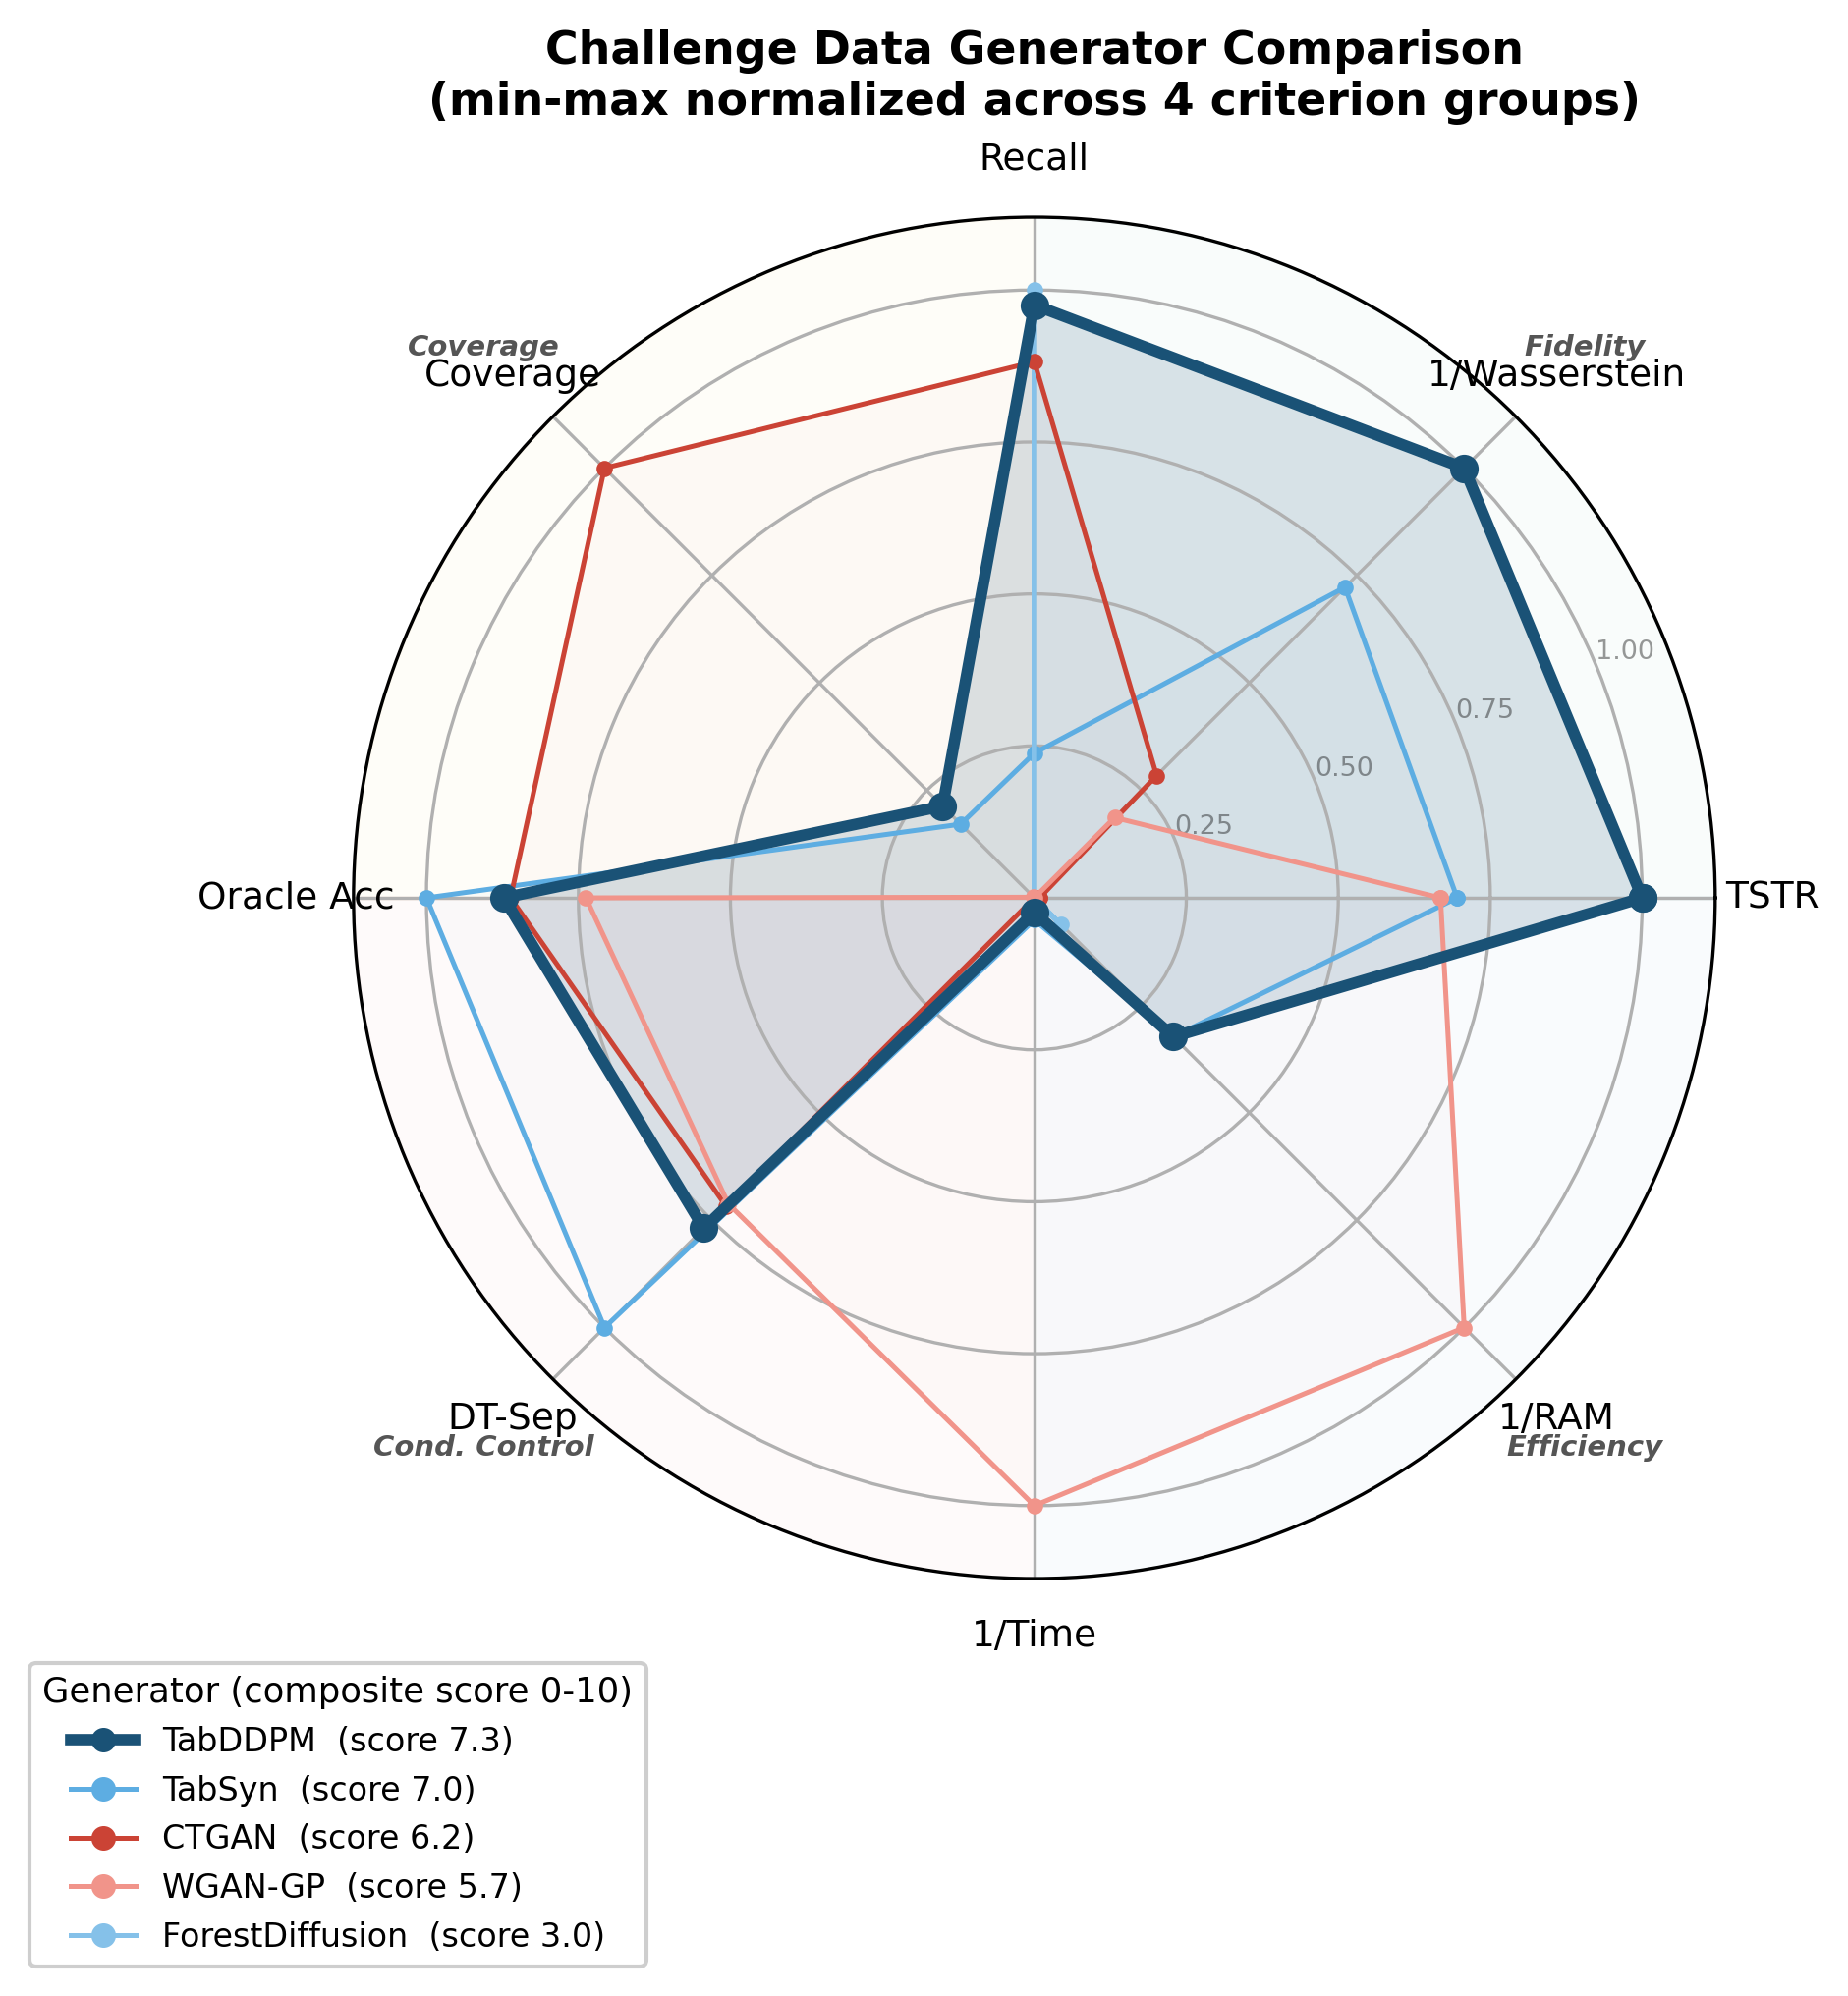
\includegraphics[width=0.85\linewidth]{Figures/fig_5_11_ab_testing_generative_models.png}
    \caption{Kết quả A/B Testing mô hình sinh dữ liệu}
\end{figure}

\subsection{Lý do TabDDPM được chọn}
TabDDPM {[}7{]} được chọn làm bộ sinh mặc định cho DT-Guard dựa trên năm lý do kỹ thuật, mỗi lý do gắn liền với yêu cầu cụ thể của hệ thống:

\textbf{(1)} TSTR cao nhất (71,4\%): đảm bảo challenge data phản ánh thực tế. TSTR (Train on Synthetic, Test on Real) đo hiệu năng của mô hình phân loại được huấn luyện trên dữ liệu tổng hợp khi kiểm tra trên dữ liệu thật. TSTR 71,4\% nghĩa là nếu dùng dữ liệu TabDDPM sinh ra để huấn luyện mô hình IDS, mô hình đó đạt 71,4\% accuracy trên dữ liệu thật, phản ánh sát thực tế. Trong DT-Guard, challenge data đóng vai trò "đề thi" để đánh giá hành vi mô hình. Nếu đề thi không phản ánh đúng phân phối thực, kết quả đánh giá sẽ sai lệch, client tốt có thể bị đánh giá thấp (trùng hợp mẫu challenge khó bất thường) hoặc client xấu được đánh giá cao (trùng hợp mẫu challenge dễ). TSTR cao đảm bảo tính đại diện của challenge data.

\textbf{(2)} Wasserstein Distance thấp nhất (0,061): phân phối sinh sát nhất. Wasserstein Distance đo khoảng cách giữa phân phối dữ liệu sinh và phân phối dữ liệu thật, giá trị càng thấp thì hai phân phối càng giống nhau. Điều này đảm bảo challenge data không chỉ đúng nhãn mà còn đúng phân phối đặc trưng trong mỗi nhãn, tránh hiện tượng sinh ra mẫu có nhãn đúng nhưng giá trị đặc trưng bất thường.

\textbf{(3)} Recall cao: bao phủ đầy đủ các lớp tấn công. Recall cao nghĩa là dữ liệu sinh bao phủ hầu hết các vùng của phân phối thực, không bỏ sót lớp tấn công nào. Điều này quan trọng vì nếu challenge data thiếu một lớp tấn công cụ thể (ví dụ: lớp Backdoor), pipeline sẽ không thể phát hiện client đầu độc nhắm vào lớp đó, client có thể phân loại sai lớp Backdoor nhưng vẫn đạt F1 cao nếu challenge data không chứa mẫu Backdoor.

\textbf{(4)} Training time nhanh (\textasciitilde200 giây): phù hợp tích hợp thực tế. TabDDPM được huấn luyện một lần duy nhất trước khi bắt đầu vòng lặp FL. Với 200 giây huấn luyện, tổng thời gian chuẩn bị (bao gồm cả sinh pre-generated challenge pool) vẫn nhỏ hơn đáng kể so với thời gian huấn luyện một round FL (\textasciitilde8,7 giây $\times$ 20 rounds = 174 giây). So với CTGAN (\textasciitilde1600 giây), TabDDPM tiết kiệm 8 lần thời gian chuẩn bị.

\textbf{(5)} Hỗ trợ conditional sampling: sinh theo nhãn chỉ định. TabDDPM cho phép sinh mẫu với nhãn cụ thể bằng cách thêm thông tin nhãn vào đầu vào mạng neural (class-conditional generation). Khả năng này cho phép tạo challenge data với phân bổ nhãn cân bằng, mỗi lớp có số mẫu tương đương, đảm bảo không có lớp nào bị thiểu số trong "đề thi." Các phương pháp không hỗ trợ conditional generation phải sinh ngẫu nhiên rồi lọc theo nhãn, tốn kém hơn và khó kiểm soát tỉ lệ.

\section{Kịch bản C: Đánh giá tính công bằng và phát hiện free-rider}

\subsection{Thiết lập kịch bản free-rider}
Để đánh giá khả năng phát hiện free-rider của DT-PW, thực nghiệm được tiến hành trên CIC-IoT-2023, đưa 4 free-rider (20\% trong 20 client) vào hệ thống. Free-rider sao chép mô hình toàn cục kèm nhiễu không đáng kể thay vì huấn luyện. Bốn chiến lược tổng hợp trọng số được so sánh: DT-PW, Trust-Score (LUP {[}5{]}), Uniform, và FedAvg.

\subsection{Kết quả so sánh}
DT-PW gán trọng số đúng 0,0 cho tất cả 4 free-rider và phân bổ đều cho 16 client thật (mỗi client 0,0625 = 1/16), đạt accuracy cao nhất 72,97\%. Effort Gate phát hiện 100\% free-rider nhờ prediction divergence gần bằng 0.

Trust-Score (LUP {[}5{]}) tạo ra hiệu ứng ngược: free-rider nhận trọng số 0,2448, cao gấp 188 lần so với client thật chỉ 0,0013. Nguyên nhân là Trust-Score đo khoảng cách tham số đến mô hình toàn cục, free-rider có tham số gần nhất nên được đánh giá "đáng tin" nhất. Hiện tượng "đảo ngược ý nghĩa" này khiến accuracy sụt xuống 46,49\%.

Uniform gán trọng số bằng nhau (0,05) cho tất cả, đạt 72,51\%, gần bằng DT-PW chỉ vì trong kịch bản này free-rider echo mô hình toàn cục nên không gây hại chủ động.

FedAvg gán trọng số theo số mẫu, hiệu quả tương tự Uniform trong kịch bản này.

\begin{figure}[H]
    \centering
    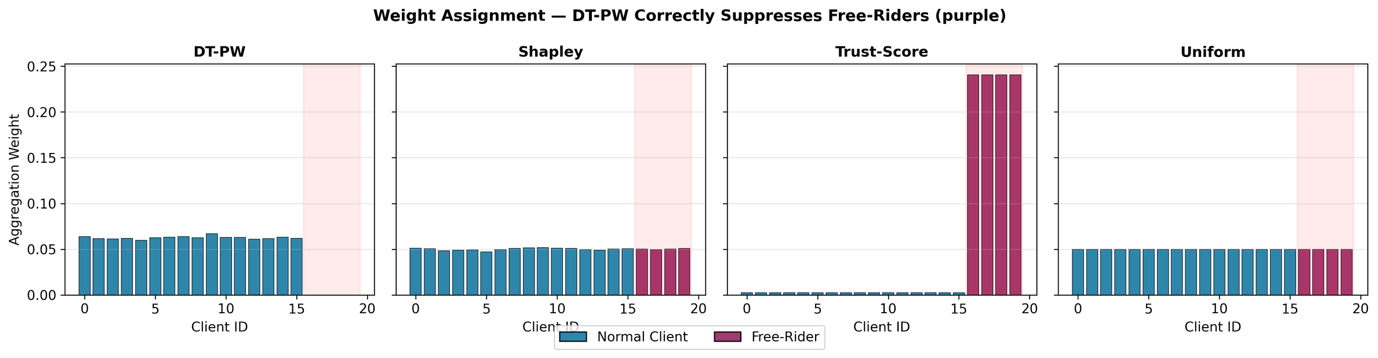
\includegraphics[width=0.85\linewidth]{Figures/fig_5_12_per_client_weight.png}
    \caption{Trọng số per-client theo từng chiến lược tổng hợp}
\end{figure}

\subsection{Phân tích}
Kết quả chứng minh ba điểm quan trọng:

\textbf{(1)} DT-PW là chiến lược duy nhất phát hiện và loại bỏ hoàn toàn free-rider, nhờ đo hành vi suy luận (prediction divergence) thay vì khoảng cách tham số.

\textbf{(2)} Trust-Score dựa trên khoảng cách tham số có lỗ hổng cấu trúc, vô tình thưởng cho free-rider. Đây là bằng chứng mạnh nhất cho thấy chỉ dựa vào đặc trưng tĩnh của tham số sẽ không phản ánh đúng đóng góp thực tế.

\textbf{(3)} DT-PW vừa đảm bảo công bằng vừa cải thiện chất lượng mô hình nhờ ưu tiên client đóng góp tri thức mới.

\section{Phân tích overhead và chi phí tài nguyên}

\subsection{Thời gian thực thi}
DT-Guard có tổng thời gian trung bình mỗi round là 8,735 giây trên CIC-IoT-2023, phân tách như sau:

\begin{itemize}
\item
  \textbf{Training per round:} 8,654 giây (chiếm 99,1\%)
\item
  \textbf{DT verification:} 0,064 giây (chiếm 0,7\%)
\item
  \textbf{DT-PW scoring:} 0,017 giây (chiếm 0,2\%)
\item
  \textbf{Tổng overhead DT-Guard:} 0,081 giây (chiếm \textless{} 1\%)
\end{itemize}

So sánh thời gian aggregation với các baseline: FedAvg 0,001 giây, Krum 0,016 giây, Median 0,037 giây, Trimmed Mean 0,019 giây, GeoMed 0,149 giây, SignGuard 0,018 giây, ClipCluster 0,020 giây, LUP 0,031 giây, PoC 0,004 giây. DT-Guard (0,081 giây) có overhead cao hơn nhưng vẫn ở mức có thể chấp nhận, nhỏ hơn 1\% tổng thời gian round.

\textbf{Phân tích nguyên nhân chi phí từng phương pháp:}

Thời gian aggregation của mỗi phương pháp phản ánh trực tiếp độ phức tạp thuật toán. FedAvg (0,001 giây) là nhanh nhất vì chỉ cần một phép tính trung bình có trọng số trên N vector tham số, thao tác O(N $\times$ d) tuyến tính đơn giản. PoC (0,004 giây) nhanh gần như FedAvg vì MMD$^{2}$ chỉ cần tính kernel distance giữa hai tập tham số, không cần lặp. Krum (0,016 giây) chậm hơn 16 lần FedAvg vì cần tính khoảng cách đôi giữa tất cả N bản cập nhật (O(N$^{2}$ $\times$ d)), rồi với mỗi update tìm k khoảng cách gần nhất, chi phí tăng bậc hai theo số client. SignGuard (0,018 giây) và ClipCluster (0,020 giây) có chi phí tương đương do đều cần tính ma trận khoảng cách (sign-based hoặc cosine) rồi thực hiện phân cụm, MeanShift hoặc Agglomerative.

Trimmed Mean (0,019 giây) cần sắp xếp N vector theo L2 norm rồi cắt hai đầu, chi phí sắp xếp O(N log N). LUP (0,031 giây) chậm hơn do thực hiện hai bước: MAD bounding (tính median và độ lệch tuyệt đối) rồi hierarchical clustering, cần xây dựng dendrogram hoàn chỉnh. Median (0,037 giây) cần sắp xếp theo từng chiều tham số, với d = 39 đặc trưng và số tham số MLP lớn (\textasciitilde90.000 tham số), việc tính trung vị cho từng chiều tạo ra chi phí đáng kể. GeoMed (0,149 giây) là chậm nhất trong các baseline, gần gấp đôi DT-Guard, do giải bài toán Weiszfeld lặp: mỗi bước cần tính khoảng cách từ mọi update đến điểm hiện tại rồi cập nhật, lặp cho đến khi hội tụ. Với dữ liệu Non-IID, điểm khởi tạo xa geometric median khiến cần nhiều vòng lặp hơn.

DT-Guard (0,081 giây) nằm giữa: chậm hơn các baseline thống kê đơn giản nhưng nhanh hơn GeoMed. Chi phí được phân bổ thành DT verification (0,064 giây), chạy inference 200 mẫu $\times$ 20 client qua mạng MLP; và DT-PW scoring (0,017 giây), chạy inference thêm một lần cho mô hình toàn cục rồi so sánh dự đoán. Tuy overhead cao hơn FedAvg 81 lần, nhưng xét trong bối cảnh tổng thời gian round (8,735 giây), 0,081 giây là không đáng kể, và lợi ích thu được (FPR = 0\%, DR 98,3\%, phát hiện 100\% free-rider) hoàn toàn vượt trội so với chi phí tăng thêm.

\begin{figure}[H]
    \centering
    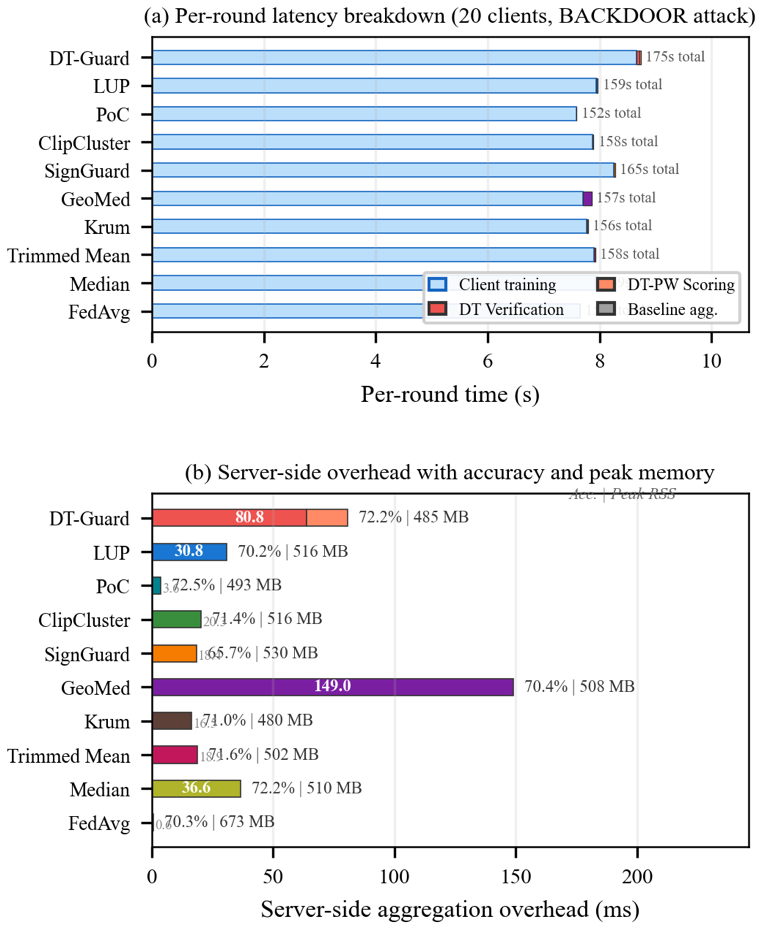
\includegraphics[width=0.85\linewidth]{Figures/fig_5_13_overhead_resource.png}
    \caption{Tổng hợp chi phí tính toán: (a) phân tích thời gian per-round và (b) overhead server-side, accuracy, peak memory theo từng phương pháp}
\end{figure}

\subsection{Bộ nhớ}
Kết quả bất ngờ là DT-Guard có peak memory thấp thứ hai: 485,34 MB, thậm chí thấp hơn FedAvg (673,09 MB). Nguyên nhân là cơ chế sandbox: Digital Twin chỉ nạp một mô hình tại một thời điểm vào bộ nhớ để kiểm thử, rồi giải phóng trước khi nạp mô hình tiếp theo (sequential loading). Trong khi đó, FedAvg và hầu hết baseline phải giữ tất cả bản cập nhật trong bộ nhớ đồng thời.

So sánh peak memory: Krum 479,50 MB, DT-Guard 485,34 MB, PoC 493,05 MB, Trimmed Mean 501,59 MB, GeoMed 507,61 MB, Median 510,28 MB, ClipCluster 515,92 MB, LUP 515,97 MB, SignGuard 530,20 MB, FedAvg 673,09 MB.

\textbf{Phân tích nguyên nhân mức tiêu thụ bộ nhớ:}

Các phương pháp phòng thủ có thể được phân thành hai nhóm theo chiến lược quản lý bộ nhớ. Nhóm 1: Giữ tất cả update đồng thời, bao gồm FedAvg, Trimmed Mean, Median, GeoMed, ClipCluster, LUP, SignGuard. Các phương pháp này cần giữ tất cả N bản cập nhật (mỗi bản \textasciitilde90.000 tham số $\times$ 4 byte = \textasciitilde360 KB) trong bộ nhớ để thực hiện tính toán (sắp xếp, phân cụm, hoặc trung bình). Với N = 20 client, tổng bộ nhớ cho tham số là \textasciitilde7,2 MB, không lớn so với mô hình, nhưng cần thêm các ma trận trung gian cho tính toán (khoảng cách đôi, phân cụm, v.v.). FedAvg có peak memory cao nhất (673 MB) vì ngoài N bản cập nhật, còn giữ bộ đệm cho tính trung bình có trọng số trên toàn bộ tham số. SignGuard (530 MB) cần thêm bộ nhớ cho ma trận sign features (pos/neg/zero cho từng chiều $\times$ N client). LUP và ClipCluster (\textasciitilde516 MB) cần thêm ma trận khoảng cách và dendrogram cho hierarchical clustering.

Nhóm 2: Sequential processing, bao gồm DT-Guard và Krum. Krum có peak thấp nhất (479,5 MB) vì chỉ cần tính khoảng cách từng update đến k update gần nhất, có thể thực hiện tuần tự mà không cần giữ toàn bộ ma trận khoảng cách trong bộ nhớ. DT-Guard (485 MB) thấp hơn đáng kể so với FedAvg nhờ cơ chế sandbox: tại mỗi thời điểm, chỉ có một mô hình client được nạp vào sandbox để chạy inference trên challenge data (200 mẫu), sau đó được giải phóng hoàn toàn trước khi nạp mô hình tiếp theo. Bộ nhớ peak xảy ra khi nạp mô hình + challenge batch + output tensors, nhưng tổng vẫn nhỏ hơn FedAvg vì FedAvg phải giữ tất cả N bản cập nhật đồng thời trong quá trình tính trung bình.

Điểm đáng chú ý là: mặc dù DT-Guard thực hiện nhiều tác vụ hơn (inference 20 client $\times$ 200 mẫu + tính Trust-Score + tính prediction divergence), tổng bộ nhớ vẫn thấp hơn các phương pháp đơn giản hơn. Đây là minh chứng cho hiệu quả của thiết kế sequential loading, đánh đổi thời gian (chạy tuần tự thay vì song song) để giảm bộ nhớ đỉnh, phù hợp với môi trường IoT nơi tài nguyên bộ nhớ hạn chế.

\subsection{Trade-off chi phí - lợi ích}
Để đánh giá toàn diện, cần đặt chi phí tăng thêm của DT-Guard trong ngữ cảnh lợi ích an ninh thu được.

\textbf{Về thời gian:} Chi phí tăng thêm 0,081 giây/round (\textless 1\% tổng thời gian) tương đương với mức overhead thấp nhất có chấp nhận được trong các hệ thống phân tán. Để hình dung, với 20 round FL, tổng thời gian huấn luyện là \textasciitilde175 giây, trong đó overhead của DT-Guard chỉ chiếm \textasciitilde1,6 giây, ít hơn thời gian một epoch huấn luyện cục bộ (\textasciitilde1,4 giây). Trong thực tế, thời gian round FL bị chi phối gần như hoàn toàn bởi huấn luyện cục bộ (99,1\%) và giao tiếp mạng (không đo trong mô phỏng), nên 0,7\% thêm cho verification là không đáng kể.

\textbf{Về bộ nhớ:} DT-Guard không những không tăng peak memory mà còn giảm xuống 485 MB so với FedAvg (673 MB), tiết kiệm 28\% bộ nhớ. Trong môi trường IoT nơi bộ nhớ RAM hạn chế, đây là lợi ích thay vì chi phí.

\textbf{Về lợi ích an ninh, so sánh trực tiếp với chi phí:}

\begin{longtable}[]{@{}
  >{\raggedright\arraybackslash}p{(\linewidth - 10\tabcolsep) * \real{0.1521}}
  >{\raggedright\arraybackslash}p{(\linewidth - 10\tabcolsep) * \real{0.1982}}
  >{\raggedright\arraybackslash}p{(\linewidth - 10\tabcolsep) * \real{0.1699}}
  >{\raggedright\arraybackslash}p{(\linewidth - 10\tabcolsep) * \real{0.1377}}
  >{\raggedright\arraybackslash}p{(\linewidth - 10\tabcolsep) * \real{0.1865}}
  >{\raggedright\arraybackslash}p{(\linewidth - 10\tabcolsep) * \real{0.1556}}@{}}
\caption{Trade-off chi phí - lợi ích giữa DT-Guard và các phương pháp đại diện} \\
\toprule\noalign{}
\begin{minipage}[b]{\linewidth}\centering
\textbf{Phương pháp}
\end{minipage} & \begin{minipage}[b]{\linewidth}\centering
\textbf{Overhead (ms/round)}
\end{minipage} & \begin{minipage}[b]{\linewidth}\centering
\textbf{Peak Memory (MB)}
\end{minipage} & \begin{minipage}[b]{\linewidth}\centering
\textbf{FPR}
\end{minipage} & \begin{minipage}[b]{\linewidth}\centering
\textbf{DR (50\% malicious)}
\end{minipage} & \begin{minipage}[b]{\linewidth}\centering
\textbf{Free-rider}
\end{minipage} \\
\midrule\noalign{}
\endfirsthead
%
\multicolumn{6}{c}{{\textit{(tiếp) Bảng 5.4}}} \\
\toprule\noalign{}
\begin{minipage}[b]{\linewidth}\centering
\textbf{Phương pháp}
\end{minipage} & \begin{minipage}[b]{\linewidth}\centering
\textbf{Overhead (ms/round)}
\end{minipage} & \begin{minipage}[b]{\linewidth}\centering
\textbf{Peak Memory (MB)}
\end{minipage} & \begin{minipage}[b]{\linewidth}\centering
\textbf{FPR}
\end{minipage} & \begin{minipage}[b]{\linewidth}\centering
\textbf{DR (50\% malicious)}
\end{minipage} & \begin{minipage}[b]{\linewidth}\centering
\textbf{Free-rider}
\end{minipage} \\
\midrule\noalign{}
\endhead
\bottomrule\noalign{}
\endlastfoot
FedAvg & 1 & 673 & N/A & Sụp \textless{} 1\% (MPAF) & Không phát hiện \\
GeoMed & 149 & 508 & Cao (LIE) & Sụp (LIE) & Không phát hiện \\
LUP & 31 & 516 & 26,7\% trung bình & 72,2\% accuracy & Thưởng (0,2448) \\
\textbf{DT-Guard} & \textbf{81} & \textbf{485} & \textbf{0\%} & \textbf{98,3\%} & \textbf{Loại (0,0)} \\
\end{longtable}

Bảng trên cho thấy GeoMed có overhead gần gấp đôi DT-Guard (149 ms vs. 81 ms) nhưng lại sụp đổ trước tấn công LIE, chi phí cao hơn mà lợi ích thấp hơn. LUP có overhead thấp hơn DT-Guard (31 ms vs. 81 ms) nhưng FPR 26,7\% và thưởng free-rider, tiết kiệm 50 ms mỗi round đổi với việc loại nhầm hơn 1/4 client lành tính là một sự đánh đổi không thể chấp nhận trong hệ thống thực. DT-Guard chi thêm 50 ms/round so với LUP nhưng thu được FPR = 0\%, DR tăng đáng kể, và phát hiện 100\% free-rider.

Kết luận: tỉ lệ chi phí/lợi ích của DT-Guard là thuận, chi phí tăng thêm (\textless 1\% thời gian, giảm 28\% bộ nhớ) hoàn toàn xứng đáng với lợi ích an ninh đạt được (FPR = 0\%, DR 98,3\%, phát hiện free-rider). Hệ thống có thể triển khai trong môi trường thực tế mà không ảnh hưởng đáng kể đến hiệu năng.

\section{Bàn luận tổng hợp}

\subsection{Tại sao DT-Guard hiệu quả?}
Hiệu quả của DT-Guard bắt nguồn từ kiểm chứng hành vi chủ động thay vì phân tích tham số thụ động. Thực nghiệm xác nhận bốn trường hợp: tấn công dù giữ tham số bình thường nhưng hành vi sai bị phát hiện, client Non-IID dù tham số lệch nhưng hành vi đúng được chấp nhận, và free-rider với prediction divergence gần 0 bị loại. Pipeline 4 lớp đánh giá toàn diện từ nhiều góc nhìn (hiệu năng phát hiện, kháng backdoor, lệch tham số, ổn định), kết hợp với fusion thích ứng và DT-PW tạo ra khả năng phân biệt mà không phương pháp đơn lẻ nào đạt được.

\subsection{Tại sao FPR = 0\%?}
FPR = 0\% là kết quả quan trọng nhất. Các phương pháp thụ động đo khoảng cách tham số: client có tham số lệch xa bị loại. Trong môi trường Non-IID, client lành tính có dữ liệu thiên lệch tự nhiên bị nhầm là tấn công. DT-Guard giải quyết nhờ kiểm chứng hành vi: client Non-IID lành tính dù tham số lệch nhưng phân loại chính xác trên challenge data $\rightarrow$ IDS Performance Score cao $\rightarrow$ vượt Trust Gate. Cơ chế fusion thích ứng đóng vai trò then chốt: trong balanced mode, IDS Performance Score (trọng số 0,7) bù cho Parameter Similarity Score thấp (trọng số 0,3).

\subsection{So sánh trực tiếp với LUP}
LUP {[}5{]} là phương pháp gần nhất về hiệu năng tổng thể, nhưng có hai hạn chế cấu trúc: (1) FPR cao (trung bình 26,7\% tại 50\% malicious) do đo khoảng cách tham số; (2) Thưởng free-rider (0,2448 vs 0,0013 cho client thật) do Trust-Score dựa trên khoảng cách. DT-Guard giải quyết cả hai vấn đề nhờ kiểm chứng hành vi và prediction divergence.

\subsection{Các hạn chế nhận diện được}
Mặc dù kết quả khả quan, DT-Guard có một số hạn chế: (1) Overhead tăng tuyến tính theo số client, với hệ thống rất lớn cần tối ưu thêm bằng parallel verification hoặc sampling; (2) Phụ thuộc chất lượng TabDDPM, nếu domain thay đổi (concept drift) mà không retrain bộ sinh, chất lượng verification giảm; (3) Chưa thử nghiệm trên mạng IoT thực tế quy mô lớn.

\section{Tổng kết chương}
Thực nghiệm trên CIC-IoT-2023 và ToN-IoT cho thấy DT-Guard duy trì accuracy ổn định, DR đạt 98,3\% (CIC-IoT-2023) và 99,5--100\% (ToN-IoT) ở 50\% malicious, FPR 0\% trên cả 5 loại tấn công ở cả hai dataset; TabDDPM đạt TSTR cao nhất (71,4\%) và Wasserstein Distance thấp nhất (0,061); DT-PW phát hiện 100\% free-rider. Overhead 80,8 ms/round (\textless 1\%) và peak memory 485 MB (thấp nhất). Kết quả này tạo nền tảng cho Chương 6.

% Chapter 6
\chapter{KẾT LUẬN VÀ KHUYẾN NGHỊ}
\label{Chapter6}

Chương này tổng kết kết quả, đóng góp khoa học, các hạn chế, và đề xuất hướng phát triển tiếp theo.

\section{Tổng kết kết quả và đóng góp khoa học}
Đề tài đã xây dựng thành công khung DT-Guard, hệ thống phòng thủ chủ động cho FL trong ngữ cảnh IoT IDS, sử dụng Digital Twin làm môi trường kiểm chứng hành vi. Kết quả thực nghiệm trên CIC-IoT-2023 (34 lớp, 39 đặc trưng, MLP) và ToN-IoT (10 lớp, 10 đặc trưng, MLP) cho thấy:

\begin{itemize}
\item
  Accuracy ổn định: 72,3\%--73,3\% trên CIC-IoT-2023, 99,8\% trên ToN-IoT qua mọi mức malicious (10\%--50\%).
\item
  Detection Rate cao: 89,5\%--98,3\% trên CIC-IoT-2023, 90\%--100\% trên ToN-IoT.
\item
  FPR = 0\%: DT-Guard duy trì FPR 0\% ở cả hai bộ dữ liệu, trong khi LUP có FPR trung bình 26,7\%.
\item
  Phát hiện free-rider: DT-PW gán trọng số 0 cho 100\% free-rider, trong khi Trust-Score (LUP) thưởng cho free-rider (0,2448 vs 0,0013).
\item
  Overhead thấp: 80,8 ms/round (\textless{} 1\%), peak memory 485 MB (thấp nhất).
\end{itemize}

Năm đóng góp khoa học: (1) Paradigm "active behavioral verification" thay thế passive parameter inspection; (2) Chứng minh tính tổng quát hóa liên dataset, baseline sụp đổ trước cùng tấn công ở cả hai dataset; (3) Giải pháp đồng thời ba vấn đề: phòng thủ đa dạng tấn công, FPR = 0\%, phát hiện free-rider; (4) Framework triển khai được với overhead thấp; (5) Hướng dẫn chọn TabDDPM làm bộ sinh qua A/B Testing, TabDDPM đạt TSTR cao nhất (71,4\%) và Wasserstein Distance thấp nhất (0,061).

\section{Các hạn chế của hệ thống}
Mặc dù kết quả thực nghiệm khả quan, DT-Guard vẫn còn một số hạn chế cần được thừa nhận:

\begin{itemize}
\item
  \textbf{(1)} Overhead tăng tuyến tính theo số client. Chi phí verification mỗi round là O(M $\times$ N), phù hợp với N = 20 client hiện tại (overhead \textless{} 1\%) nhưng sẽ tăng đáng kể khi mở rộng ra hệ thống quy mô lớn (N = 1000+). Cần kết hợp parallel verification và sampling để giảm tải.
\item
  \textbf{(2)} Chưa đánh giá trên mạng IoT thực tế. Toàn bộ thực nghiệm chạy trên môi trường mô phỏng tuần tự {[}1, 2, 5, 15, 16, 18, 19{]}, không bao gồm độ trễ mạng, mất gói tin, client dropout, và sự không đồng nhất về tài nguyên, các yếu tố phổ biến trong triển khai thực.
\item
  \textbf{(3)} Chưa thử nghiệm tấn công adaptive và FL bất đồng bộ. Đề tài chưa đánh giá adaptive attacks, tấn công được thiết kế để vượt qua DT-Guard, và chưa thử nghiệm trong mô hình FL bất đồng bộ (asynchronous FL) {[}22{]}, nơi mô hình toàn cục liên tục thay đổi.
\end{itemize}

\section{Hướng phát triển tiếp theo}
Dựa trên các hạn chế trên, đề tài đề xuất các hướng phát triển:

\textbf{(1)} Tích hợp Blockchain cho audit log bất biến {[}21{]}. Ghi nhận Trust-Score và quyết định verification lên chain để đảm bảo tính minh bạch và kiểm toán.

\textbf{(2)} Triển khai trên testbed IoT thực tế. Đánh giá trên môi trường vật lý gồm nhiều thiết bị IoT khác nhau để kiểm chứng tính khả thi khi có độ trễ mạng và tài nguyên hạn chế.

\textbf{(3)} Quy mô lớn: parallel và hierarchical verification. Chạy nhiều DT instance song song, kết hợp sampling chỉ kiểm chứng ngẫu nhiên một tỉ lệ client mỗi round. Mở rộng sang kiến trúc phân cấp (edge $\rightarrow$ fog $\rightarrow$ cloud).

\textbf{(4)} Mở rộng sang FL bất đồng bộ. Điều chỉnh Trust Gate so sánh với snapshot mô hình toàn cục tại thời điểm nhận update, và điều chỉnh Effort Gate cho ngưỡng divergence phù hợp.

\section{Kết luận luận văn}
Luận văn đã đề xuất và đánh giá hệ thống DT-Guard, phương pháp phòng thủ chủ động cho Federated Learning trong ngữ cảnh phát hiện xâm nhập IoT, sử dụng Digital Twin làm môi trường kiểm chứng hành vi.

\textbf{Về mặt khoa học}, đóng góp quan trọng nhất là chuyển dịch phòng thủ FL từ phân tích tham số thụ động sang kiểm chứng hành vi chủ động. Ba khoảng trống nghiên cứu đã được giải quyết: phòng thủ hiệu quả trước năm loại tấn công, phân biệt chính xác Non-IID và đầu độc, phát hiện và loại bỏ free-rider.

\textbf{Về mặt thực nghiệm}, kết quả trên CIC-IoT-2023 và ToN-IoT xác nhận tính hiệu quả và tổng quát hóa của DT-Guard: accuracy ổn định bất chấp tỉ lệ độc hại tăng, DR đạt 98,3\% và 99,5--100\% ở 50\% malicious, FPR = 0\% trên toàn bộ 40 kịch bản, phát hiện 100\% free-rider, overhead dưới 1\%.

\textbf{Về mặt ý nghĩa}, nguyên lý kiểm chứng hành vi chủ động là hướng triển vọng cho hệ thống FL an toàn trong IoT IDS. Lỗ hổng của phương pháp thụ động mang tính cấu trúc: cùng một baseline thất bại trước cùng loại tấn công ở cả hai môi trường, chứng tỏ vấn đề nằm ở bản chất cách tiếp cận.

\textbf{Về công bố khoa học}, kết quả cốt lõi của luận văn đã được đệ trình tại hội nghị quốc tế IEEE ICCE 2026 (Eleventh International Conference on Communications and Electronics), với tiêu đề "Active Digital Twin Verification for Robust Federated Learning in IoT Intrusion Detection" {[}23{]} (hiện đang trong quá trình chờ duyệt).


\clearpage
\phantomsection
\addcontentsline{toc}{chapter}{Tài liệu tham khảo}
\begin{thebibliography}{99}
\bibitem{ref1} Baruch M., Baruch G., Goldberg Y. (2019), "A little is enough: Circumventing defenses for distributed learning", Advances in Neural Information Processing Systems (NeurIPS), Vol.32.
\bibitem{ref2} Blanchard P., El Mhamdi E. M., Guerraoui R., Stojanovic R. J. (2017), "Machine learning with adversaries: Byzantine tolerant gradient descent", Advances in Neural Information Processing Systems (NeurIPS), Vol.30.
\bibitem{ref3} Cao W., Gong X. Y., Zhenqiang N. (2022), "MPAF: Model poisoning attacks to federated learning based on fake clients", Proc. IEEE/CVF Conference on Computer Vision and Pattern Recognition Workshops (CVPRW), pp.3396--3404.
\bibitem{ref4} Gulrajani I., Ahmed F., Arjovsky M., Dumoulin V., Courville A. C. (2017), "Improved training of Wasserstein GANs", Advances in Neural Information Processing Systems (NeurIPS), pp.5767--5777.
\bibitem{ref5} Issa W., Moustafa N., Turnbull B., Choo K.-K. R. (2025), "DT-BFL: Digital twins for blockchain-enabled federated learning in Internet of Things networks", Ad Hoc Networks, Vol.165, Art. no.103632.
\bibitem{ref6} Jolicoeur-Martineau A., Fatras K., Kachman T. (2024), "Generating and imputing tabular data via diffusion and flow-based gradient-boosted trees", Proc. 27th International Conference on Artificial Intelligence and Statistics (AISTATS), pp.1288--1296.
\bibitem{ref7} Kotelnikov A., Baranchuk D., Rubachev I., Babenko A. (2023), "TabDDPM: Modelling tabular data with diffusion models", Proc. 40th International Conference on Machine Learning (ICML), pp.17564--17579.
\bibitem{ref8} Lu Y., Huang X., Zhang K., Maharjan S., Zhang Y. (2020), "Communication-efficient federated learning and permissioned blockchain for digital twin edge networks", IEEE Internet of Things Journal, Vol.8 (4), pp.2276--2288.
\bibitem{ref9} McMahan B., Moore E., Ramage D., Hampson S., Arcas B. A. (2017), "Communication-efficient learning of deep networks from decentralized data", Proc. 20th International Conference on Artificial Intelligence and Statistics (AISTATS), pp.1273--1282.
\bibitem{ref10} Moustafa N. (2021), "A new distributed architecture for evaluating AI-based security systems at the edge: Network TON\_IoT datasets", Sustainable Cities and Society, Vol.72, Art. no.102994.
\bibitem{ref11} Neto E. C. P., Dadkhah S., Ferreira R., Zohourian A., Lu R., Ghorbani A. A. (2023), "CICIoT2023: A real-time dataset and benchmark for large-scale attacks in IoT environment", Sensors, Vol.23 (13), Art. no.5941.
\bibitem{ref12} Pillutla K., Kakade S. M., Harchaoui Z. (2022), "Robust aggregation for federated learning", IEEE Transactions on Signal Processing, Vol.70, pp.1142--1154.
\bibitem{ref13} Qu Y., Pokhrel S., Nepal S., Gao L., Xiang Y. (2021), "Decentralized privacy using blockchain-enabled federated learning in fog computing", IEEE Internet of Things Journal, Vol.8 (8), pp.6521--6533.
\bibitem{ref14} Shapley L. S. (1953), "A value for n-person games", Contributions to the Theory of Games II, Princeton University Press, Princeton, NJ, USA, pp.307--317.
\bibitem{ref15} Shejwalkar V., Houmansadr A. (2021), "Manipulating the Byzantine: Optimizing model poisoning attacks and defenses for federated learning", Proc. 28th Network and Distributed System Security Symposium (NDSS).
\bibitem{ref16} Xu J., Huang S.-L., Song L., Lan T. (2022), "SignGuard: Byzantine-tolerant federated learning through collaborative malicious gradient filtering", Proc. IEEE 42nd International Conference on Distributed Computing Systems (ICDCS), pp.530--540.
\bibitem{ref17} Xu L., Skoularidou M., Cuesta-Infante A., Veeramachaneni K. (2019), "Modeling tabular data using conditional GAN", Advances in Neural Information Processing Systems (NeurIPS), Vol.32.
\bibitem{ref18} Yin D., Chen Y., Kannan R., Bartlett P. (2018), "Byzantine-robust distributed learning: Towards optimal statistical rates", Proc. 35th International Conference on Machine Learning (ICML), pp.5650--5659.
\bibitem{ref19} Zeng Y. et al. (2024), "ClipCluster: A defense against Byzantine attacks in federated learning", IEEE Transactions on Information Forensics and Security, Vol.19, pp.4567--4581.
\bibitem{ref20} Zhang H., Zhang J., Srinivasan B., Shen Z., Qin X., Faloutsos C. (2024), "Mixed-type tabular data synthesis with score-based diffusion in latent space", Proc. 12th International Conference on Learning Representations (ICLR).
\bibitem{ref21} Zhang X., Liu H., Yang F. (2025), "Enhanced traffic carbon emissions data sharing and modeling via blockchain and personalized federated learning in IIoT ecosystem", IEEE Internet of Things Journal, Vol.12 (15), pp.31064--31078.
\bibitem{ref22} Zhang Z., Peng H., Li L., Bao S. (2025), "Adaptive asynchronous federated learning for digital twin driven smart grid", IEEE Transactions on Smart Grid, Vol.16 (5), pp.4167--4181.
\bibitem{ref23} Pham Hoang Hao, Phan The Duy, Pham Van-Hau (2026), "Active Digital Twin Verification for Robust Federated Learning in IoT Intrusion Detection", Proc. 2026 Eleventh International Conference on Communications and Electronics (ICCE 2026) --- Communication Networks and Systems, IEEE, Nha Trang, Vietnam.
\end{thebibliography}


\appendix
\clearpage
\phantomsection
\addcontentsline{toc}{chapter}{Bài báo công bố}
\markboth{}{}
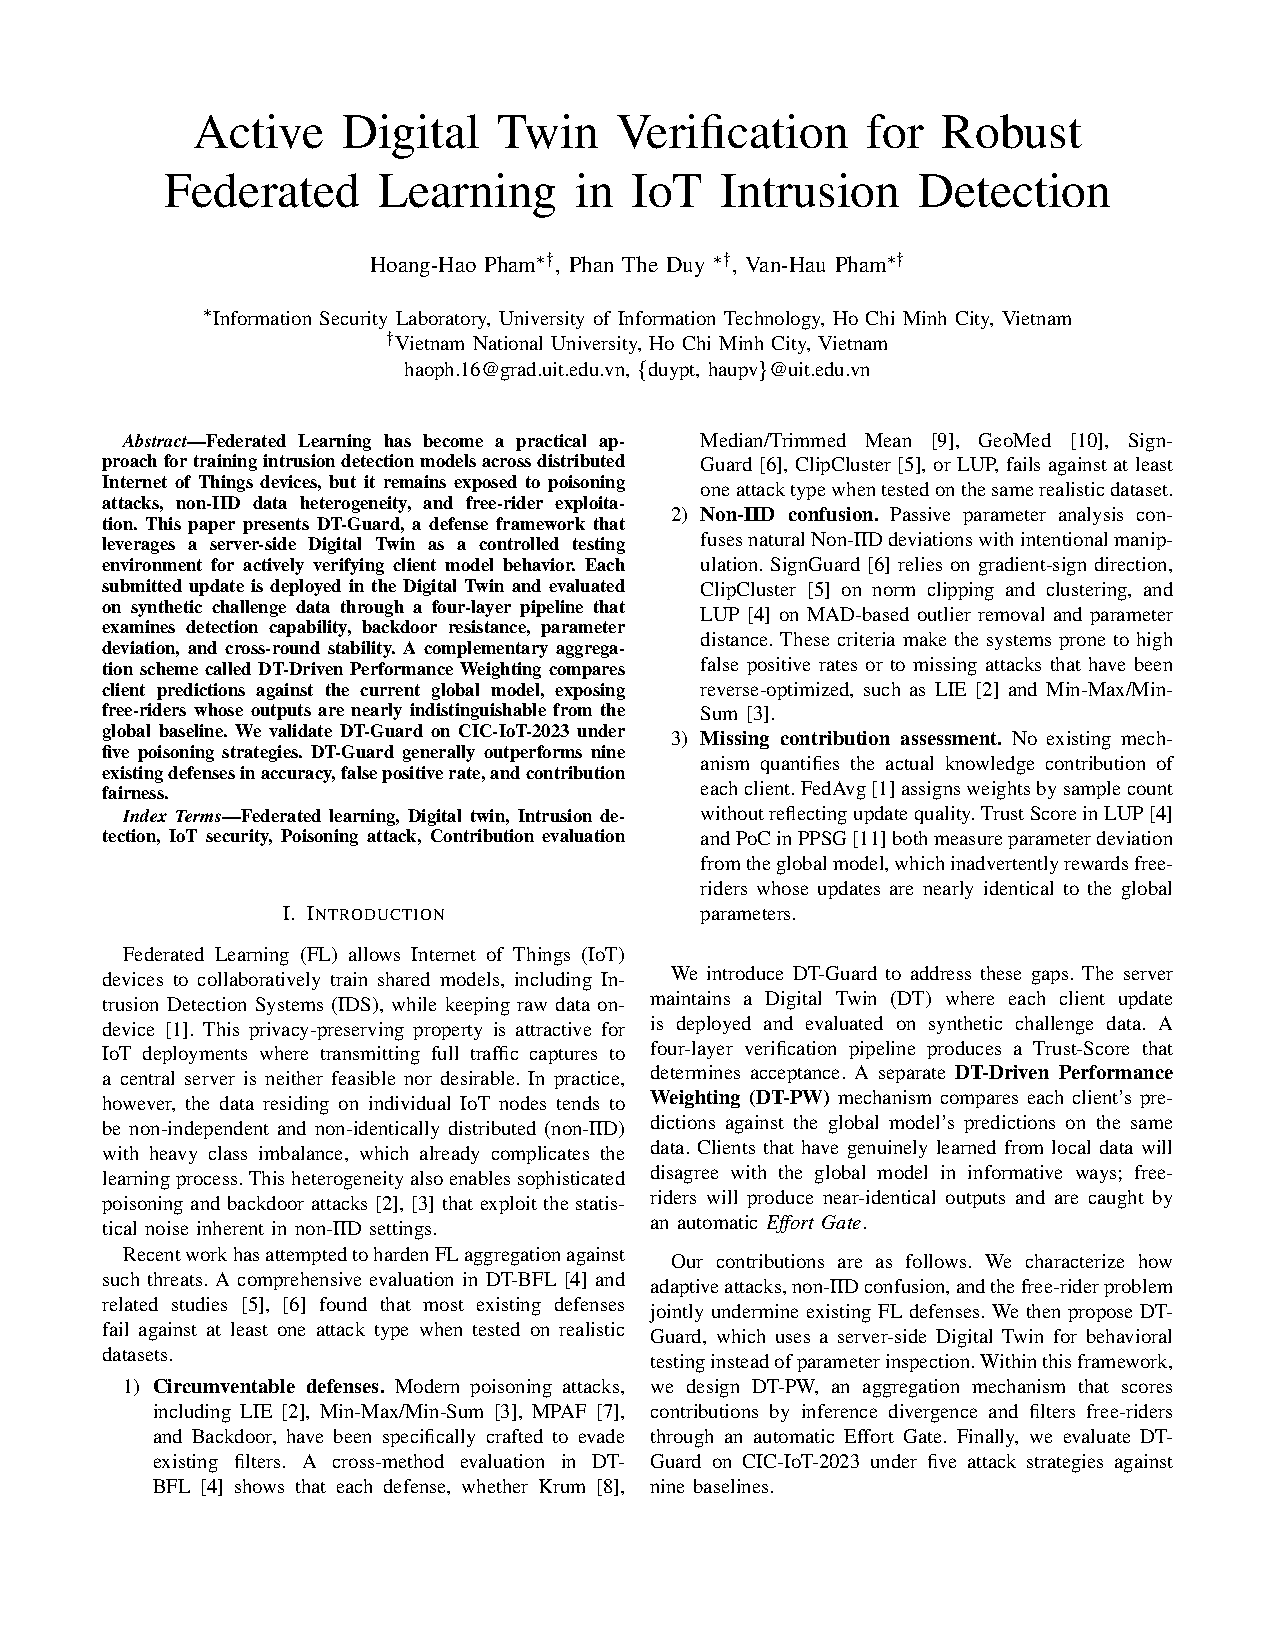
\includepdf[pages=-, scale=0.95, pagecommand={\thispagestyle{empty}}]{IEEE_ICCE_paper.pdf}

\end{document}
